% !Mode:: "TeX:UTF-8"
\documentclass[fontset=fandol,type=doctor,campus=harbin,tocfour=false]{hithesisbook}
\usepackage{hithesis}
\usepackage{etoolbox}

\usepackage{amssymb}
\usepackage{pifont}% 供表格符号 \ding 使用
% \usepackage{adjustbox}
% \usepackage{subcaption}
\usepackage{tikz}
\usepackage{placeins}
\usetikzlibrary{arrows.meta,positioning}
\graphicspath{{figures/}}
\def\tableofengcontents{} % 去掉博士英文目录（不产生空白页）

% 表格常用符号
\DeclareRobustCommand{\xchen}[1]{#1}% 论文中的红色标注（此处做空处理）
\def\Checkmark{\ding{51}}
\def\XSolidBrush{\ding{110}}


% UPA 论文专用命令
\newcommand{\selectionname}{Adaptive Pseudo-label Selection}
\newcommand{\selectshortname}{APS}
\newcommand{\clname}{Class-Aware Contrastive Learning}
\newcommand{\clshortname}{CACL}
\newcommand{\shortname}{UPA}

% DAMF 论文专用命令（用于chap3消融表中引用方法短名）
\newcommand{\disname}{Alternating Distillation}
\newcommand{\shortdisname}{ADL}
\newcommand{\adaname}{Adaptive Prompt Tuning}
\newcommand{\shortadaname}{APT}

% ===== 编译开关（调试时取消注释；定稿前请恢复注释）=====
% \includeonly{body/chap2, body/chap3,back/conclusion}
% \includeonly{back/conclusion}
% \includeonly{body/chap5}
% 多章：  % \includeonly{body/chap2,body/chap3}

% ===== 调试开关：注释掉下面这行使图片正常编译，取消注释则图片区域变为空白但保持占位高度 ======
\usepackage{letltxmacro}
\LetLtxMacro\originalincludegraphics\includegraphics
\renewcommand{\includegraphics}[2][]{\typeout{DBG: skipping \detokenize{#2}}\phantom{\originalincludegraphics[#1]{#2}}}

\begin{document}

\frontmatter
% !Mode:: "TeX:UTF-8"

\hitsetup{
  %******************************
  % 注意：
  %   1. 配置里面不要出现空行
  %   2. 不需要的配置信息可以删除
  %******************************
  %
  %=====
  % 秘级
  %=====
  statesecrets={公开},
  natclassifiedindex={TM301.2},
  intclassifiedindex={62-5},
  %
  %=========
  % 中文信息
  %=========
  ctitlecover={面向多泛化场景的模型迁移研究},%放在封面中使用，自由断行
  ctitle={面向多泛化场景的模型迁移研究},%放在原创性声明中使用
  % csubtitle={一条副标题}, %一般情况没有，可以注释掉
  cxueke={工学},
  csubject={计算机科学与技术},
  caffil={计算学部},
  cauthor={陈希},
  csupervisor={姚鸿勋教授},
  % cassosupervisor={某某某教授}, % 副指导老师
  % ccosupervisor={某某某教授}, % 联合指导老师
  % 如果是第一封面的日期要手动设置，需要取消注释下一行，并将内容改为“规范”中要求的封面第一页最下方的日期
  % firstpagecdate={2022年6月},
  % 日期自动使用当前时间，若需指定按如下方式修改：
  % cdate={超新星纪元},
  cstudentid={9527},
  cstudenttype={学术学位论文}, %非全日制教育申请学位者
  cnumber={no9527}, %编号
  cpositionname={哈铁西站}, %博士后站名称
  cfinishdate={20XX年X月---20XX年X月}, %到站日期
  csubmitdate={20XX年X月}, %出站日期
  cstartdate={3050年9月10日}, %到站日期
  cenddate={3090年10月10日}, %到站日期
  %（同等学力人员）、（工程硕士）、（工商管理硕士）、
  %（高级管理人员工商管理硕士）、（公共管理硕士）、（中职教师）、（高校教师）等
  %
  %
  %=========
  % 英文信息
  %=========
  etitle={Research on Model Transfer in Multi-Generalization Scenarios},
  esubtitle={This is the sub title},
  exueke={Engineering},
  esubject={Computer Science and Technology},
  eaffil={\emultiline[t]{Faculty of Computing}},
  eauthor={Xi Chen},
  esupervisor={Prof. Hongxun Yao},
  % eassosupervisor={XXX},
  % 日期自动生成，若需指定按如下方式修改：
  % edate={December, 2017},
  estudenttype={Master of Art},
  %
  % 关键词用“英文逗号”分割
  ckeywords={模型迁移；多泛化场景；样本挖掘；多模态监督；语义理解标准},
  ekeywords={Model Transfer; Multi-Generalization Scenarios; Sample Mining; Multimodal Supervision; Semantic Understanding Standards},
}

\begin{cabstract}

视觉感知模型从封闭实验环境走向真实开放场景的过程中，需要应对训练与部署之间多层面的差异。视觉感知任务在预训练—微调范式下已取得显著进展，然而大规模预训练模型在训练阶段所接触的样本分布、类别词表与语义定义，往往与目标部署环境存在系统性偏差：这种偏差不仅体现在数据的统计特性上，也体现在类别集合的开放程度与语义刻画的精细程度上。当模型从实验室走向真实环境时，缺乏目标标注条件下的分布差异持续存在、已知与未见类别在开放环境中共存、高阶语义因主观多义而难以仅由结论判定等问题相互交织，使得模型的可靠迁移成为制约感知系统实际落地的核心瓶颈。本文将此类由训练与部署条件不一致引发的稳健性问题概括为多泛化场景，并依据偏移发生的空间层次将其划分为域泛化、类泛化与语义泛化三个层面，三者依次对应特征与样本空间、类别空间与语义空间的偏移，围绕不同偏移维度、监督资源约束和模型载体，研究模型知识向目标任务的可靠迁移与可诊断评测。

围绕多泛化场景下的模型迁移，本文沿样本表征、类别概念与高阶语义三个层次展开研究。面向数据分布变化的域泛化场景，研究无监督与少监督条件下的目标域适应；面向类别词表开放的类泛化场景，研究未见类别的识别与像素级定位；面向语义理解要求提升的任务场景，构建分层评测协议，考察多模态大语言模型能否依据视觉证据作出情感解释。前两类研究着重提升模型的迁移能力，后一类研究刻画已有能力在高阶语义任务中的适用范围。主要研究内容如下：

首先，面向跨域分布偏移下的无监督模型迁移场景，模型既要在目标域维持稳定的判别表征，也要避免错误预测在自训练中被反复强化。现有伪标签方法常依据预测置信度或固定阈值选择样本，但域偏移下的高置信预测仍可能出错；与此同时，骨干网络对源域纹理、背景及空间共现的依赖可能削弱目标表征的稳定性。在源数据不可访问、目标标签缺失的设定下，这两类不确定性更难借助真实标签或源样本加以校正。为此，本文沿监督信号与表征建模两条路径展开研究：提出基于特征空间邻居一致性的自适应伪标签筛选方法，以邻居分布估计样本级可靠性，并通过类别感知对比学习抑制噪声传播；进一步提出基于选择性扫描的不确定性感知迁移方法，利用通道级视觉状态空间模块与语义一致性打乱策略，缓解通道建模不足和虚假相关性累积，以线性复杂度实现长程跨域建模。两项研究在 Office-Home、VisDA-C、Office、DomainNet-126 四个基准上分别将精度提升至 81.7\%、89.3\%、93.3\%、77.9\%，取得了具有竞争力的迁移性能。

其次，面向少监督模型迁移场景，有限监督的核心挑战在于如何提高每一份目标域标注的学习收益，使模型在分布偏移下仍获得可靠判别能力。现有方法分别着力于有限标注的获取或利用，尚难同时兼顾目标样本的覆盖性、不同知识来源的互补性，以及监督信息向目标模型能力的转化。视觉—语言模型能够提供与源模型互补的开放语义先验，但其潜力仍取决于目标域适配与有效的跨模型交互。在主动标注预算有限的具体设定下，本文提出基于多模态基础模型引导的双主动学习方法，通过双聚焦样本选择、视觉—语言模型适配与交替蒸馏，促进源模型与视觉—语言模型之间的双向知识传递，并以协作风险上界分析样本覆盖、模型风险及跨模型对齐对目标性能的影响。在 Office-Home、VisDA-C、Office 闭集设定下，该方法较最优基线分别提升 4.5、1.5、0.6 个百分点，在开集设定下分别提升 9.7、3.5、1.0 个百分点。

再次，面向开放词汇分割任务，模型既要识别训练阶段未见的类别，也要准确界定其像素区域。现有两阶段方法通常先生成类别无关掩码、再进行语义分类，掩码与类别判别所依赖的特征难以充分对齐；单阶段方法虽简化流程，仍受图文对齐模型缺乏像素级监督的限制。分割基础模型具有较强的空间定位能力，却不能独立提供开放词汇语义。针对两类先验在掩码质量与类别判别上的能力错配，本文提出跨模型先验融合方法，在轻量解码器中通过查询与特征注入融合空间定位和类别语义信息，并在推理阶段集成分割基础模型的零样本掩码预测，以改善未见类别的分割质量。该方法在全景分割、语义分割和实例分割等八个基准上验证了其泛化能力。

最后，面向艺术情感推理任务，目标任务从事实识别延伸到情感归因与证据化解释，模型生成的流畅描述并不必然具有可靠的视觉依据。现有视觉情感数据集和美学评测多关注情感标签、属性评分或描述质量，难以区分模型是否识别了支撑情感判断的感知线索，也难以定位从感知到推理的具体失效环节。针对这一评测缺口，本文构建多层级基准 AER-Bench，将艺术情感理解拆解为感知维度、情感与效价—唤醒—支配、基于证据的推理、情感描述四个互补层级，并结合结构化题目与开放式评分进行诊断。该基准覆盖 2{,}058 件艺术作品、34{,}791 道评测题目；对 14 个代表性多模态大语言模型的系统评测揭示了情感判断与证据化解释之间的能力差距。

综上，本文围绕多泛化场景下的模型迁移，形成了从跨域稳定表征、开放类别识别到高阶语义能力评测的研究路径：通过无监督与少监督适应提升跨分布迁移的可靠性，通过跨模型先验融合增强未见类别的细粒度识别，并以多维评测协议刻画多模态大语言模型在证据化语义理解中的能力边界。

\end{cabstract}
\begin{eabstract}

  As visual perception models move from closed experimental environments to open real-world scenarios, they must cope with multifaceted discrepancies between training and deployment. Visual perception tasks have achieved remarkable progress under the pre-training--fine-tuning paradigm, yet the sample distributions, category vocabularies, and semantic definitions encountered by large-scale pretrained models during training often differ systematically from those in target deployment environments: such discrepancies are manifested not only in the statistical properties of data, but also in the openness of category sets and the granularity of semantic characterization. When models are transferred from laboratories to real-world settings, distributional discrepancies that persist in the absence of target annotations, the coexistence of known and unseen categories in open environments, and high-level semantics that cannot be judged by the final prediction alone become intertwined, making reliable model transfer a central bottleneck for the practical deployment of perception systems. This dissertation refers to such robustness issues arising from inconsistencies between training and deployment conditions as \emph{multi-generalization scenarios}, and partitions them according to the spatial level at which the shift occurs into three interlocking levels of domain, category, and semantic generalization, which correspond in turn to shifts in feature and sample space, category space, and semantic space. The reliable transfer and diagnosable evaluation of model knowledge for target tasks are investigated under different shift dimensions, supervision-resource constraints, and model carriers.
  
  Taking model transfer under multi-generalization scenarios as its research line, this dissertation focuses on three generalization challenges arising in the transition from training to deployment, namely domain distribution shift, the coexistence of open-set categories, and high-level semantic understanding, and organizes the research of the dissertation accordingly. At the domain-generalization level, this dissertation studies how unlabeled target data can be exploited reliably under constrained supervision resources, and develops both unsupervised and weakly supervised transfer methods. At the category-generalization level, this dissertation studies the semantic coverage of models when the category set is no longer closed, and develops open-vocabulary segmentation methods for unseen categories. At the semantic-generalization level, this dissertation studies whether the model's judgments of emotion and other semantics genuinely rely on the visual evidence in the image, and develops evaluation protocols with stratified diagnostic capability. The three levels progress in turn and jointly point toward the reliable deployment of visual perception models. The main research contents are as follows:
  
  First, to suppress uncertainty in unsupervised model transfer, this dissertation investigates the reliable quantification and control of cross-domain transfer uncertainty. To mitigate the accumulation of transfer uncertainty caused by pseudo-label noise, an adaptive pseudo-label filtering method based on neighborhood consistency is proposed. The method estimates sample-level uncertainty from neighborhood distributions to adaptively select high-quality pseudo-labels. To address two inherent limitations of state-space models, namely insufficient channel modeling and the accumulation of spurious correlations, an uncertainty-aware transfer method based on selective scanning is further proposed. By incorporating a channel-wise visual state-space module and a semantic-consistent shuffling strategy, the method enables efficient long-range cross-domain modeling with linear complexity. On the Office-Home, VisDA-C, Office, and DomainNet-126 benchmarks, the proposed methods achieve accuracies of 81.7\%, 89.3\%, 93.3\%, and 77.9\%, respectively, demonstrating competitive transfer performance.
  
  Second, this dissertation addresses information maximization in weakly supervised model transfer, namely maximizing the amount of information that the model acquires from the supervisory signals under a limited annotation budget. Existing methods lack systematic exploration of supervisory signals from multimodal pretrained models in both sample selection and model learning, fail to convert the complementary information across channels into learning gains of the target model, and have not established a rigorous theoretical framework for characterizing information content and for bidirectional deep collaboration between vision--language models and source models. To this end, a dual active learning method guided by multimodal foundation models is proposed. Through sample-selection design, multimodal model adaptation, and alternating distillation, the method achieves bidirectional deep collaboration between source models and vision--language models in the hypothesis space. On the closed-set settings of Office-Home, VisDA-C, and Office, it improves upon the strongest baselines by 4.5, 1.5, and 0.6 percentage points, respectively; on the open-set settings, the corresponding improvements are 9.7, 3.5, and 1.0 percentage points.
  
  Third, to deeply exploit multimodal category priors for model generalization, this dissertation investigates multi-stream semantic alignment and spatial-localization reasoning optimization. Image--text alignment models tend to emphasize global semantics while producing coarse mask boundaries, whereas foundation segmentation models excel at localization but lack semantic generalization. Moreover, these two types of priors are difficult to deeply integrate within a unified decoding framework. To address this capability mismatch, a cross-model prior fusion method is proposed. It achieves deep fusion of spatial-localization and semantic features within a lightweight decoder, and incorporates zero-shot mask predictions from a foundation segmentation model through an open-set ensemble module during inference, thereby improving the segmentation quality of unseen categories. The proposed method validates its generalization capability for unseen categories on eight benchmarks spanning panoptic, semantic, and instance segmentation.
  
  Finally, to establish multidimensional standards for semantic understanding, this dissertation studies a multi-level evaluation protocol for art emotion reasoning, enabling distinguishable diagnosis between fluent emotional descriptions and their reliable grounding in visual evidence in higher-level semantic scenarios. To address the lack of fine-grained diagnostic capability in existing visual-emotion benchmarks for differentiating fluent emotional expression from evidence-grounded explanation, AER-Bench, a multi-level benchmark for art emotion reasoning, is constructed. It decomposes art emotion understanding into four complementary levels: perceptual dimensions; emotion together with valence, arousal, and dominance; evidence-grounded reasoning; and emotion description. AER-Bench contains 2{,}058 artworks and 34{,}791 evaluation questions, and has been used to systematically evaluate 14 representative multimodal large language models.
  
  In summary, this dissertation systematically investigates model transfer in multi-generalization scenarios from the perspectives of domain, category, and semantic generalization. At the domain-generalization level, it studies unsupervised and weakly supervised model transfer: the former mitigates transfer uncertainty by suppressing noisy pseudo-labels and their propagation, whereas the latter leverages open-semantic priors from multimodal models to drive sample mining and cross-modal collaborative transfer. At the category-generalization level, it investigates multi-stream semantic alignment and spatial-localization reasoning optimization, integrating the localization and semantic priors of heterogeneous models to improve fine-grained recognition of unseen categories. At the semantic-generalization level, it establishes multidimensional semantic-understanding standards by constructing evaluation protocols that jointly support evidence anchoring and multidimensional diagnosis, thereby providing interpretable evaluation criteria for open semantic scenarios.
  
  \end{eabstract}

\makecover
% 符号说明表：置于摘要之后、目录之前
% !Mode:: "TeX:UTF-8"
% 全文符号说明表：位置在中文摘要之后、目录之前。
% 收录标准：仅保留正文（body/、back/、extras/）中出现频次较高、或对理解方法必需的符号；
% 低频符号（仅出现 1--2 次）不单独列出，读者可由正文就近定义处获知。
% 表格编号在本环境内重置为“表 1 / 表 2 …”。

\makeatletter
\renewcommand{\hit@denotation@ctitle}{符号说明表}
\renewcommand{\hit@denotation@etitle}{List of Symbols and Notations}
\makeatother
\begin{denotation}
\vspace{-1.5em}
\begin{longtable}{@{}p{0.28\textwidth}p{0.64\textwidth}@{}}
\toprule
\textbf{符号} & \textbf{含义} \\
\midrule
\endfirsthead
\multicolumn{2}{@{}l}{\small\itshape 符号说明表（续）}\\
\toprule
\textbf{符号} & \textbf{含义} \\
\midrule
\endhead
\midrule
\multicolumn{2}{@{}r}{\small\itshape 接下页}\\
\endfoot
\bottomrule
\endlastfoot

\addlinespace[1.0ex]
\multicolumn{2}{@{}l}{\itshape 数据、空间与分布}\\
\addlinespace[0.3ex]
$\mathcal{X}$ / $\mathcal{Y}$ / $\mathcal{C}$ & 样本空间 / 标签空间 / 类别集合 \\
$C$ & 类别数，$|\mathcal{Y}| = C$ \\
$x$ / $y$ & 样本 / 标签 \\
$n_s$ / $n_t$ & 源域 / 目标域样本数 \\
$\mathcal{S}$ / $\mathcal{T}$ & 源域数据集（带标签）/ 目标域数据集（无标签） \\
$\mathcal{T}_c$ / $\mathcal{T}_q$ & 干净伪标签样本集 / 主动标注的目标样本子集 \\
% $\mathcal{T}_{\text{CO}}$ / $\mathcal{T}_{\text{MH}}$ & Core-Set 点集 / MH 点集 \\
$\mathcal{D}_l$ & 已标注数据集合，$\mathcal{D}_l = \mathcal{S} \cup \mathcal{T}_q$ \\
$P$ / $Q$ & 目标域分布 / 源域分布 \\
$\mathcal{Z}$ & 视觉—语言模型的特征空间 \\
$d_X$ / $d_Z$ / $d_Y$ & 分别定义于 $\mathcal{X}$、$\mathcal{Z}$、$\mathcal{Y}$ 上的距离函数 \\
$d(\cdot,\cdot)$ & 余弦相似度 \\

\addlinespace[1.0ex]
\multicolumn{2}{@{}l}{\itshape 模型与多模态表示}\\
\addlinespace[0.3ex]
$\theta_s$ / $\theta_t$ / $\theta_v$ & 源域模型 / 目标域模型 / 视觉—语言模型 \\
$g$ / $f$ & 特征提取器 / 分类器 \\
$\mathrm{Enc}_t(\cdot)$ & 视觉—语言模型的文本编码器 \\
$\mathbf{I}$ / $\mathbf{w}_k$ / $V_k$ / $c_k$ & 图像特征 / 文本嵌入 / 类别 $k$ 的可学习 prompt 模板 / 类别名称 \\
$z_i$ & 归一化特征，$z_i = g(x_i)/\|g(x_i)\|$ \\
% $U$ / $\tilde{U}$ & 原始 patch 序列 / 打乱后的扰动序列 \\
% $L_{\text{vss}}$ & 通道级视觉状态空间模块的块数 \\

\addlinespace[1.0ex]
\multicolumn{2}{@{}l}{\itshape 假设空间与理论}\\
\addlinespace[0.3ex]
$\mathcal{H}$ / $\mathcal{G}$ & 源模型 / 视觉—语言模型的假设空间 \\
$h$ / $g_V$ & 假设空间 $\mathcal{H}$ / $\mathcal{G}$ 中的假设 \\
$L$ / $M$ / $\mu$ / $k$ / $k_V$ & 标量损失函数 / 损失上界 / 损失的 Lipschitz 常数 / 源假设与视觉—语言假设的 Lipschitz 常数 \\
$\eta_{\mathcal{H}}$ / $\eta_{\mathcal{G}}$ & 源模型 / 协同设定下的理想最大误差 \\
$\mathfrak{R}_{n_t}$ & Rademacher 复杂度 \\
$\epsilon$ / $\delta$ & 误差容忍度 / 置信水平参数 \\

\addlinespace[1.0ex]
\multicolumn{2}{@{}l}{\itshape 损失项与超参数}\\
\addlinespace[0.3ex]
$\mathcal{L}$ & 可训练的总损失 \\
$\mathcal{L}_{\text{ent}}$ / $\mathcal{L}_{\text{div}}$ / $\mathcal{L}_{\text{IM}}$ & 熵最小化项 / 多样性正则项 / 信息最大化项 \\
% $\mathcal{L}_{\text{CL}}$ / $\mathcal{L}_{\text{CE}}$ / $\mathcal{L}_{\text{KL}}$ / $\mathcal{L}_{\text{kg}}$ & 类感知对比学习损失 / 交叉熵损失 / KL 一致性正则 / 知识保持正则 \\
% $\mathcal{L}_C$ / $\mathcal{L}_T$ / $\mathcal{L}_V$ & 交叉熵与知识保持项之和 / 交替蒸馏中目标模型与视觉—语言模型的蒸馏损失 \\
% $\mathcal{L}_{T\leftarrow V}^{dist}$ / $\mathcal{L}_{V\leftarrow T}^{dist}$ & 交替蒸馏的目标模型 / 视觉—语言模型分支的蒸馏项 \\
$K$ / $B_{\text{batch}}$ / $\beta_{\text{CE}}$ & 近邻数 / 迷你批大小 / 交叉熵损失的权重 \\
% $\gamma_{\text{sel}}$ / $\gamma_{\text{bg}}$ / $\tau$ & 置信样本筛选比例 / 背景 patch 打乱比例 / 温度参数 \\
$B$ / $\rho$ & 标注预算 / 采样比例 \\
$N$ / $\beta_q$ & 每类保留的高置信样本数 / 标注样本权重 \\
% $\mathcal{X}_{\text{top}}$ / $\hat{\mathcal{T}}_t$ & 目标模型每类内高置信样本集合 / 已知类别样本掩码 \\
$\eta$ / $\lambda$ & 学习率 / 损失权重 \\

% \addlinespace[0.9ex]
% \multicolumn{2}{@{}l}{\itshape 开放词汇分割（第 4 章）}\\
% % \addlinespace[0.3ex]
% $F_{\text{clip},l}$ / $F_{\text{clip},e}$ / $F_{\text{sam}}$ & CLIP 图像编码器的多尺度特征 / 掩码特征 / SAM 的细粒度空间特征 \\
% $T_{\text{clip}}$ / $P_d$ / $P_{\text{cl}}$ & CLIP 文本特征 / 检测器类别预测 / CLIP 类别预测 \\
% $L_{\text{dec}}$ / $N_q$ / $\mathcal{M}$ / $\mathcal{M}^l$ & 解码器层数 / 可学习查询数 / 最终掩码族 / 第 $l$ 层掩码预测 \\
% $E_m$ / $E_p$ / $E_{\text{aux}}$ / $E_c$ & 掩码预测投影 / 空间查询投影 / 掩码辅助投影 / 类别嵌入投影 \\
% $\alpha_{\text{ens}}$ / $\beta_{\text{ens}}$ / $\epsilon_{\text{fuse}}$ & 类别集成的平衡系数 / 掩码集成的融合权重 \\

% \addlinespace[0.9ex]
% \multicolumn{2}{@{}l}{\itshape 情感评测（第 5 章）}\\
% % \addlinespace[0.3ex]
% $\mathcal{O}_{\text{per}}$ / $\mathcal{O}_{\text{emo}}$ & 感知维度标注对象 / 情感归因标注对象 \\
% $\mathcal{O}_{\text{rea}}$ / $\mathcal{O}_{\text{des}}$ & 证据锚定推理标注对象 / 情感描述标注对象 \\
% $H_{\text{KW}}$ / $V$ / $\epsilon^2$ & Kruskal--Wallis 检验统计量 / Cramer's V 列联系数 / 效应量 \\
% $\alpha_{\text{top3}}$ / $p_{\text{pen}}$ & 情感 Top-3 排序得分的加权系数 / 跨越中性点的惩罚系数 \\
% $\kappa_w$ / $n$ & 二次加权 Cohen 系数 / 样本量 \\

\end{longtable}
\vspace{0.5em}
\end{denotation}

\tableofcontents

\mainmatter

% !Mode:: "TeX:UTF-8"

\chapter[绪论]{绪论}[]

\label{chap:1}

\section{研究背景及意义}

\subsection{研究背景}

深度神经网络在计算机视觉领域的诸多基准任务上取得了令人瞩目的成绩，ImageNet、COCO 等大规模标注数据上的识别精度接近甚至超越人类水平，但其性能突破的背后隐含着一个常被忽视的前提：训练数据与测试数据服从独立同分布~\cite{liang2021source}。在真实部署中，目标侧条件可能在数据分布、类别词表或任务语义要求上偏离训练条件，由此引发三类在抽象层次上逐级递进的稳健性问题。图~\ref{fig:iidood} 对比了三类变化下的训练条件、目标条件及模型所需能力。

\begin{figure}[!htbp]
 \centering
 \includegraphics[width=.8\linewidth]{figures/multi_generalization_shift.pdf}
 \bicaption[fig:iidood]{}{训练与目标条件在数据分布、类别词表和语义要求上的差异}{Fig.}{Differences between training and target conditions in data distribution, category vocabulary, and semantic requirements}
\end{figure}

数据分布维度的失配是最直观且被研究最为广泛的一类稳健性问题。深度神经网络在训练过程中习得的并非纯粹的类别语义表征，而是将语义信息与源域的纹理风格、光照条件、采集设备特征等多层次信息深度纠缠地编码于同一特征空间~\cite{ganin2016domain,long2015learning}。这种纠缠根源于经验风险最小化在独立同分布假设下对源域损失的直接优化。过参数化的网络倾向于记忆源域样本的表面统计而非学习真正可泛化的语义不变特征，使得跨域时分类器权重所定义的判别方向在源域最优而在目标域系统性偏移。这种偏移进一步导致模型在目标域的预测不仅精度下降，还伴随显著的高置信度错误风险，例如softmax 输出对未知样本仍给出接近 1.0 的伪置信，使决策难以被阈值过滤或人工干预~\cite{liang2021source,yang2021neighbor}。在更严苛的无源设定下，源域数据因隐私法规、商业机密或存储成本等约束不可访问，模型需在源数据完全缺位的条件下仅凭源模型参数中编码的知识完成跨域传递，而由于深度特征的纠缠本质，我们无法从模型参数中直接辨识哪些知识可迁移、哪些是源域特定的虚假相关，进一步加剧了迁移的不确定性，所以就需要结合目标域数据进一步做不确定分析。
本文将这种需要将模型部署到数据分布偏移的场景称之为“域泛化”场景，与文献~\cite{zhou2023domain}中特指模型在源域完成泛化而部署时完全不接触任何目标数据的域泛化设定在前提假设上并不等同。

类别词表维度的失配是另一类广泛存在却长期被低估的稳健性问题。传统深度分类器在架构层面预设了闭集假设，即分类头的输出维度等于训练类别数，其判别性表征也是在固定类别索引上优化得到的~\cite{radford2021learning}。这一架构选择带来双重约束：一方面，分类头的权重矩阵与固定的 N 个类别索引强绑定，新类别没有对应的输出通道；另一方面，骨干网络针对 N 类判别任务优化，并未在特征空间中为未知类别预留结构化空间~\cite{kundu2022towards}。当目标场景的类别集合发生扩展、缩减或漂移时，分类头的维度结构与新类别空间在维度上不再兼容，已训练模型的判别能力在新类别上无法直接复用，并倾向于将未知样本强行归入概率最高的已知类别，产生高置信度的错误预测。这一现象在自动驾驶、工业质检等在线服务场景中尤为危险~\cite{kirillov2023segment}。为缓解这一约束，基于图文对比预训练的开放词汇分类器通过引入语言空间的语义先验扩展了类别边界，但其语义覆盖仍受限于预训练文本编码器的词表，难以覆盖长尾、新兴或专业领域类别~\cite{radford2021learning}。逐类重新采集、专家标注并重训模型的过程伴随显著的时间与资金投入，在隐私敏感与不可中断的业务场景中，这种``重训窗口''往往根本不可行~\cite{kirillov2023segment}。这要求识别模型能够在训练时未见过的新类别上完成判别，而传统固定词表架构在维度不兼容的设定下难以直接扩展，尤其在像素级分割任务中，新类别的精细空间定位对像素级标注成本与模型先验的开放语义能力同时提出要求，使类别词表维度的失配在通用识别研究中成为一个关键挑战。

语义层次维度的失配是相较前两者更高阶的稳健性问题。现有视觉基础模型（特别是多模态大语言模型）的预训练以事实型图文描述为主，习得的表征擅长回答“图像中有什么”这类可枚举的类别问题~\cite{mmbench2023}，却对隐含于视觉元素与文化语境、风格表征、符号解读之间的关联缺乏结构化编码，其流畅的语义表述多源于训练语料的统计相关而非基于视觉证据的可靠推理~\cite{achlioptas2021artemis,zhao2014exploring}。具体而言，预训练语料中的图像描述通常以物体、场景、动作等可枚举事实为骨架，而高阶情感与文化推理所需的细粒度证据化标注（如“左上方冷色笔触营造孤寂氛围”）在大规模数据中极为稀缺~\cite{aesexpert2024}，导致模型缺乏从局部视觉元素到整体情感语义的可追溯推理路径，其生成结果常表现为“流畅的虚构”——语言流畅、符合人类表达习惯，但缺乏对具体视觉元素的精确指涉~\cite{eemobench2025}。当识别任务从事实判断升级到“图像为何传达某种情感”、“差异由哪些视觉线索驱动”等需要感知能力与文化语境相融合的高阶推理时，模型所依赖的不再是可枚举的类别标签或显式物体事件，而是隐含在视觉元素与文化符号之间的语义关联。以艺术图像的情感推理为例，情感表达隐含于构图、笔触、风格化与文化符号之中，不同艺术流派的笔触技法与色彩配置所引发的情感反应具有显著的领域特异性~\cite{yang2023emoset}。然而现有通用多模态大语言模型评测基准多聚焦于事实识别层面~\cite{mmbench2023}，缺乏面向情感理解与证据化推理的结构化诊断协议，使得流畅的情感表述与基于视觉证据的可靠解释难以被精准区分~\cite{eemobench2025}，阻碍了视觉基础模型在高阶语义推理方向上的能力迭代。

综上，本文将模型在数据分布、类别词表或任务语义要求发生变化时仍需保持相应能力的这类情形统称为多泛化场景。三类变化分别要求模型维持跨域判别能力、识别未见类别，以及在事实识别之外完成有视觉证据支撑的高阶语义解释。本文从变化维度、目标侧条件和模型载体三个方面刻画这些场景：变化维度包括数据分布、类别词表与任务语义要求；目标侧条件包括无标签数据、有限人工标注，以及仅用于评测的目标任务样本；模型载体包括判别式视觉模型与多模态大语言模型（Multimodal Large Language Model, MLLM）。前两类研究通过目标域适应或跨模型融合改善迁移表现；第三类研究在不更新模型的条件下，以系统评测诊断已有能力面对更高层级语义任务时的适用范围与失效环节。
% 纯评测在此是研究方式，并非与无标注、少量标注并列的监督强度。

围绕上述多泛化场景，本文沿域泛化、类泛化与语义理解泛化三个层面展开研究。域泛化以数据分布变化为核心，面向判别式视觉模型在无标注或少量标注条件下的可靠迁移：前者通过伪标签去噪和鲁棒表征学习抑制迁移过程中的误差累积，后者利用多模态先验引导主动样本选择，以有限标注获得更高效的适应收益。类泛化进一步关注类别词表的开放变化，结合多模态先验与多基础模型协同，提升对新颖类别的识别和像素级定位能力。语义理解泛化则关注目标任务由事实识别扩展至情感归因与证据化解释时，MLLM 已有能力能否适用；本文通过多层级评测协议刻画其表现与失效环节，而不将评测结果解释为模型优化后的迁移增益。


\subsection{研究意义}
多泛化场景下的模型迁移，体现为研究对象从样本表征、类别概念到高阶语义的逐步拓展。数据分布维度（对应域泛化）关注像素风格、成像条件与统计特性的变化，核心在于学习具有跨域稳定性的表征；类别词表维度（对应类泛化）关注模型对未见类别的语义覆盖能力，核心在于实现开放环境下的识别与泛化；语义层次维度（对应语义理解泛化）关注模型能否超越事实层面的对象判别，完成情感归因、证据关联与高阶推理。
随着目标条件由分布变化扩展到类别开放，再到语义理解要求提升，模型所需保持的能力也从稳定判别延伸至新类识别与证据化解释。这一由表征到概念、再到语义的研究主线，既贯穿本文各章，也为复杂开放环境下的模型适应与能力评测提供了共同的问题框架。

\noindent\textbf{（1）域泛化方面} 

模型能否将训练阶段获得的知识有效迁移至分布不同的目标域，是迁移学习长期关注的核心问题~\cite{liang2021source,ganin2016domain,long2015learning}。棘手的是，深度表征中所蕴含的可迁移成分与域特异性成分在缺乏显式分解机制的条件下彼此纠缠，仅靠目标域自监督信号难以可靠地区分二者，伪标签噪声放大与判别性偏移是这一困境在方法层面的集中体现~\cite{yang2021neighbor,kundu2022towards}。同时，受数据隐私、版权保护和传输成本等现实因素影响，源域样本往往难以获取，使迁移过程中的可靠性诊断更具挑战。因此，研究源数据受限乃至不可访问条件下的可靠迁移机制，一方面有助于深化对无源域适应和少监督域适应中伪标签去噪、有效样本选择与鲁棒表征学习机制的认识；另一方面也能够为面向真实部署环境的目标域特征学习与高效适应策略提供方法依据。

\noindent\textbf{（2）类泛化方面} 

视觉识别系统在实际应用中面对的不再是封闭且预定义的类别集合，而是持续扩展的开放词汇空间。新物体、新材质、新场景不断涌现，固定训练词表及其对应的分类决策边界班一覆盖开放环境中的识别需求~\cite{kirillov2023segment,radford2021learning}。当模型遭遇训练阶段未见的类别时，往往会将其错误归入已有类别，并产生高置信度预测~\cite{kundu2022towards}。由此，开放词汇视觉识别的关键在于缓解封闭训练词表与开放识别需求之间的结构性错配。研究如何在缺乏目标类别标注的条件下发挥多模态基础模型的开放语义先验，并构建异质模型之间的协同机制，有助于揭示语义知识与空间定位知识的互补规律。这不仅能够为开放词汇分类、检测和分割模型的设计提供方法支撑，也有望降低模型适应新类别时对大规模重新训练和人工标注的依赖。

\newpage
\noindent\textbf{（3）语义理解泛化方面} 

多模态大语言模型已在多类事实型视觉识别任务中展现出较强能力，但在情感、意图、文化语境和审美判断等高阶语义任务中，其能力边界仍有待系统刻画~~\cite{mmbench2023,achlioptas2021artemis,eemobench2025}。这一挑战的深层原因在于：模型的预训练语料以可枚举的事实型图文描述为主，缺乏将局部视觉元素与整体情感语义相连接的可追溯推理路径~\cite{zhao2014exploring,aesexpert2024}；其语言流畅性往往源于训练统计相关而非视觉证据支撑~\cite{eemobench2025}。构建面向高阶视觉语义的基准化评测协议，是模型迁移研究在纯评测条件下的重要延伸：当目标任务缺少可用于进一步训练的监督信息时，评测能够刻画和诊断模型既有知识能否有效迁移至新的语义理解任务。此类评测不仅可为多模态大语言模型的能力诊断和后续优化提供量化依据，也有助于揭示视觉智能从感知走向认知仍然缺失的关键能力，从而推动视觉基础模型向更可靠、更具证据支撑的高阶语义推理发展。将高阶语义理解沿感知、情感、推理与描述四个多维互补层级分别考察，使语义层面的能力边界既可被定位也可被比较。

\section{国内外研究现状}

\subsection{面向域泛化场景的跨域不变特征学习}

真实场景中的光照、拍摄设备、视角和图像风格会随环境变化，使同一类别的目标呈现不同外观。域适应研究因此关注：模型能否在这些变化下保留与类别相关的判别信息，避免过度依赖特定数据域中的背景或纹理。本节所讨论的跨域不变特征学习，正是指在源域与目标域分布不同时，学习仍能支持目标域识别的视觉表征。

跨域不变性的实质是使特征对域的变化保持不敏感：同一类别的样本无论来自哪个域，都应保留与类别相关的判别结构，而不被特定域的背景、纹理与风格所主导。这一性质能否成立，既取决于模型能否构造出跨域可用的监督信号，也取决于骨干网络能否在特征生成阶段即削弱域偏移的影响。
基于上述分析，域适应研究相应地在迁移机制与骨干架构两个方向上积累了工作，前者包含分布对齐、自训练及有限标注的利用，决定模型如何借助可用数据适应目标域；后者涉及模型对局部细节与长程依赖的建模方式，影响跨域不变特征的捕获能力。下面先梳理无监督设定下的迁移机制与骨干架构演进，再讨论监督信号稀缺时相关机制的发展。

\subparagraph{无监督域适应方法}

无监督模型迁移中的不确定性，是指源域模型面对目标域分布变化、且缺乏目标标签校验时，特征表征与预测结果的可靠性难以保证。它既可能来自模型对源域纹理、背景等域特异性线索的依赖，也可能表现为目标样本预测或聚类结果的不稳定。伪标签噪声是这种不确定性在自训练监督环节的具体表现。当错误预测被当作目标域标签反复用于更新，误差便可能进一步改变特征空间，导致后续伪标签继续偏移。因此，不确定性抑制需要同时关注监督信号是否可信，以及产生该信号的表征是否稳定。

无监督域适应（Unsupervised Domain Adaptation, UDA）方法按其核心机制可划分为五大类：基于领域分布差异对齐的方法~\cite{sun2016deep,chen2019maximum}，通过度量并最小化源域与目标域在特征空间或像素空间的分布距离实现跨域对齐；基于对抗的方法DANN~\cite{ganin2016domain}，借助域判别器引导特征提取器生成域不变表征；基于重构的方法~\cite{ghifary2016deep,bousmalis2017domain}，通过图像或特征重构分解域相关与类相关成分；基于样本生成的方法~\cite{sankaranarayanan2018generate}，借助生成对抗网络或扩散模型合成目标域风格样本以缓解域偏移；以及基于自学习的方法~\cite{SRDC,SimNet,xie2018unsupervised}，其核心思想是通过源域标签样本引导，为无标签目标样本分配伪标签，再以迭代自训练或聚类方式进行精炼。具体而言，SRDC~\cite{SRDC} 通过判别性聚类揭示目标数据的内在结构；SimNet~\cite{SimNet} 通过类别原型相似度进行分类；Xie 等人~\cite{xie2018unsupervised} 进一步将自训练与样本加权相结合。上述五类方法均依赖源域训练样本在适应阶段持续可访问，构成了无监督域适应方法的主体谱系。

\begin{figure}[!htbp]
    \setlength{\tabcolsep}{0pt}
    \centering
    \subfigure[DANN框架图~\cite{DANN}]{%
    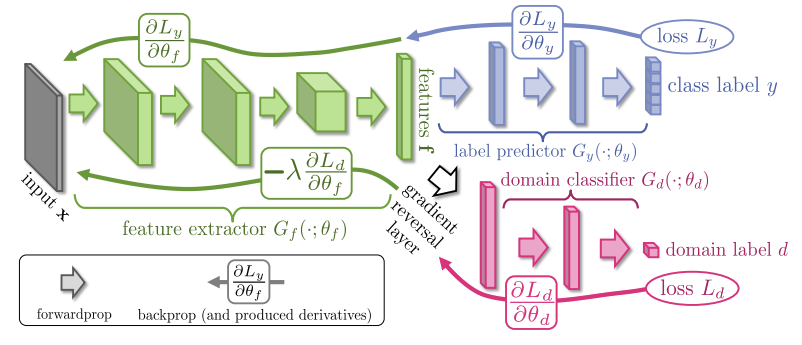
\includegraphics[width=0.48\linewidth]{figures/related_work/DANN.png}%
    }\hfill
    \subfigure[SHOT机制~\cite{liang2021source}]{%
    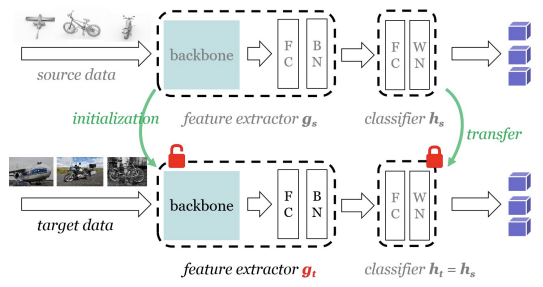
\includegraphics[width=0.48\linewidth]{figures/related_work/SHOT.png}%
    }
    \bicaption[fig:da_works]{}{域迁移代表方法}{Fig.}{Representative methods for domain adaptations}
\end{figure}

在 UDA 方法谱系之上，进一步收紧至“源数据不可访问”这一严格设定，即得到无源域适应（Source-Free Domain Adaptation, SFDA）~\cite{liang2021source}。该设定下，原有方法所依赖的源数据统计量、域判别信号、跨域重构样本与伪标签生成机制均无法直接调用，必须在仅有源模型参数的条件下构造新的跨域监督。源假设迁移（Source-Hypothesis Transfer, SHOT）~\cite{liang2021source} 通过冻结源分类器对目标特征聚类生成伪标签，成为该方向的开创性工作；NRC~\cite{yang2021neighbor} 利用邻居关系约束类内一致性；CoWA-JMDS~\cite{cowa}、U-SFAN~\cite{U-SFAN} 引入模型不确定性或数据不确定性估计对伪标签进行加权；D-MCD~\cite{chu2022denoised} 通过双分类器对抗训练识别高置信度样本中的噪声；VDM-DA~\cite{tian2022vdm} 借助虚拟域判别器选择熵值较低的干净伪标签；SSNLL~\cite{chen2022self} 以指数滑动平均模型对样本进行分层处理；Kundu 等人~\cite{kundu2022towards} 进一步从信息瓶颈角度给出 SFDA 目标风险的显式上界，为上述方法提供理论解释。


骨干网络的设计深刻影响实例级跨域不变特征的捕获能力，呈现出从 CNN 局部感受野到 ViT 全局注意力、再到选择性扫描状态空间模型（State-Space Model, SSM）Mamba 线性长程建模的清晰演进脉络。CNN（尤其是 ResNet~\cite{he2016deep}）凭借层次化特征聚合的归纳偏置~\cite{yang2021neighbor,xia2021adaptive,zhang2024nami}，是大量域迁移的默认选择；然而固定局部感受野难以捕获跨区域对象结构关系~\cite{long2015learning,ganin2016domain}。针对这一局限，ViT~\cite{dosovitskiy2021image} 通过自注意力机制实现全局感受野~\cite{sanyal2023stable,xia2024dual}，DSIT~\cite{sanyal2023dsit}、TransDA~\cite{TransDA}、C-SFTrans~\cite{sanyal2024aligning}、DPC~\cite{dpc} 等工作将 ViT 引入域适应；但 $\mathcal{O}(N^2)$ 的注意力复杂度在高分辨率图像上带来难以承受的计算开销~\cite{zhu2024vision}。作为替代，Vim~\cite{zhu2024vision}、VMamba~\cite{vmamba} 将 Mamba 扩展到视觉建模，通过双向与四向扫描策略以线性复杂度实现全局感受野~\cite{zhu2024vision,vmamba}。在域适应场景下，DA-Mamba~\cite{DA-Mamba} 进一步将 Mamba 引入跨域目标检测任务，缓解 CNN 的全局语义忽略与 ViT 的高计算开销。综合而言，沿骨干架构从 CNN 到 ViT 再到 SSM 的演进路径，跨域不变特征的捕获机制在骨干维度上得到了系统探索，为上述各类迁移方法提供了差异化的表征基础。

\subparagraph{少监督域适应方法}

当源—目标域差异较大时，仅靠全无标注的自学习路径难以进一步压缩目标域误差，一种自然思路是在迁移过程中引入少量人工标注以提升监督信号的可靠性，由此衍生出少监督域适应方法。与无监督设定相比，少监督条件下的跨域不变特征学习面临一项额外困难：可用的监督信号极为有限，模型不仅要从目标域自身挖掘可用信息，还需判断有限的人工标注应当投向何处，才能使跨域后同类样本的判别结构尽可能保持完整。

少监督设定下的核心问题可归结为监督信号的信息量问题，其含义是在给定的监督预算约束下，模型从可获得的监督信号中获取的信息量最大，即训练所得模型对目标域未知标注函数的逼近能力最强。与跨域不变性相联系，稀疏监督并不改变不变性的判据，却放大了获得不变特征所需的监督信号量：有限的标注若投向价值不足的样本，既难以覆盖目标域的真实分布，也难以纠正模型对域特异性线索的错误依赖，跨域后同类样本的判别结构便难以保持稳定。因此，样本的选择与监督信号的使用方式共同决定了该设定下的迁移效果。

基于上述问题，少监督域适应研究沿着监督信号的来源展开，回答有限标注从何而来、如何投放。据此可划分为四种典型设定：标注样本由训练集预先给定的半监督域适应（Semi-Supervised Domain Adaptation, SSDA）及其在极低监督下的极端收紧形态——少样本域适应（Few-Shot Domain Adaptation, FSDA），对应源域可访问、标注预算固定分配的常见场景；标注样本由模型在无标注目标域池中主动筛选的主动域适应（Active Domain Adaptation, ADA），对应源域可访问、标注预算由模型主导分配的场景；以及在上述任一形式上进一步收紧至“源数据不可访问”假设的主动无源域适应（Source-Free Active Domain Adaptation, SFADA）。

% SSDA/FSDA 与 ADA 在标注来源维度上互补，SSDA/FSDA/ADA 与 SFADA 在源域可见性维度上递进收紧，共同构成少监督域适应方法的两条正交设计维度。四者之间并非等量并存：SSDA 与 FSDA 因其设定明确、任务经典而积累最为充分，ADA 随后成为独立的研究方向，而 SFADA 由于源数据不可访问与标注预算受限的双重约束，直到近年才形成专门的研究脉络。

\begin{figure}[!htbp]
    \centering  
    \setlength{\tabcolsep}{0pt}
    \subfigure[MME学习框架~\cite{saito2019semi}]{
        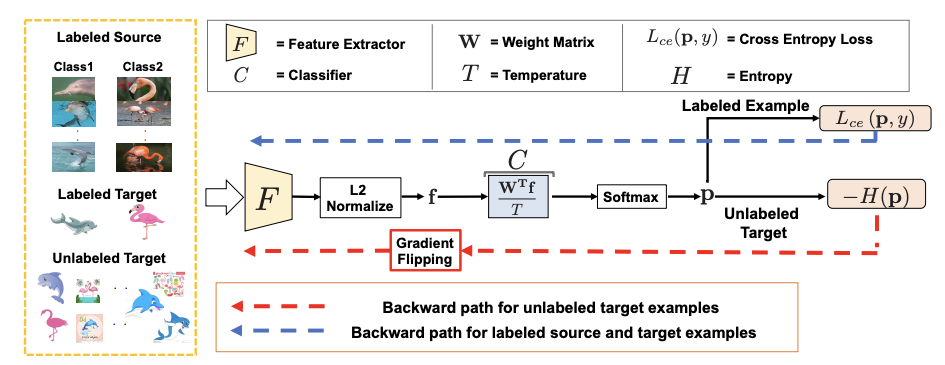
\includegraphics[width=0.48\linewidth]{figures/related_work/MME.png}
    }\hfill
    \subfigure[MHPL样本选择~\cite{MHPL}]{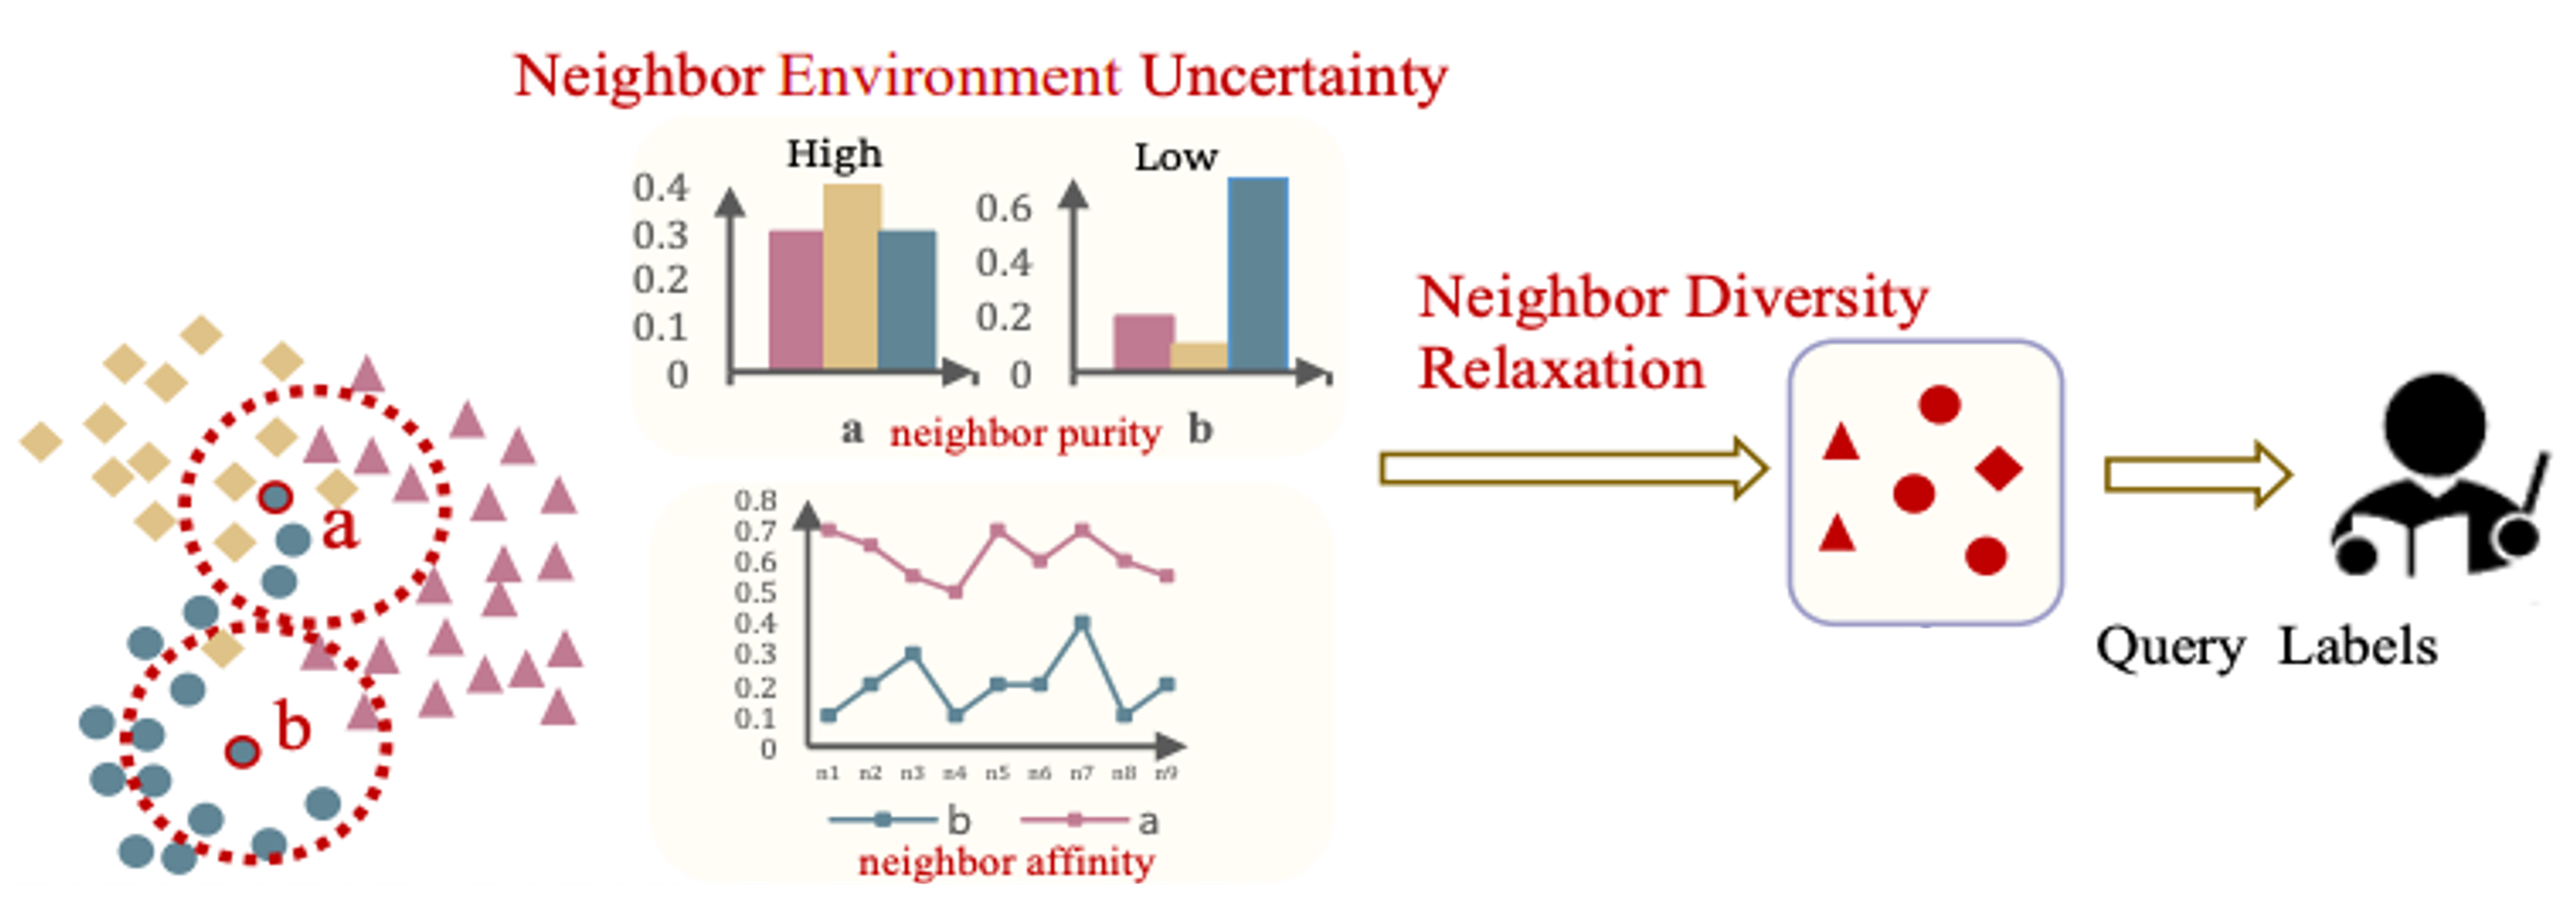
\includegraphics[width=0.48\linewidth]{figures/related_work/MHPL.png}}
    \bicaption[fig:rare_da]{}{少监督域适应代表方法}{Fig.}{Representative methods for limited-supervision domain adaptation}
\end{figure}

半监督SSDA与少样本FSDA域适应设定了有限标注目标样本（每类 1 至 N 个）+ 大量无标注目标样本的标准少监督范式，是少监督域适应方法谱系中最一般化的形式。SSDA 的开创性工作 MME~\cite{saito2019semi} 通过对抗式最小化最大熵同时利用标注与无标注目标样本的边缘分布；后续工作进一步围绕伪标签去噪、对比约束与一致性正则等机制扩展 SSDA 设定下的跨域监督构造。FSDA 进一步收紧至每类仅 1–5 个标注目标样本的极端设定，借助度量学习、元学习或跨域原型对齐缓解极低监督下的过拟合问题~\cite{zhao2021fewshot}。

上述设定下，信息最大化以不同程度地发挥作用。标注预先给定时，它体现为如何充分利用既有的标注与大量无标注目标样本构造有效监督，使有限的先验信息在训练中得到充分兑现；标注由模型筛选时，它还进一步体现为有限的人工标注应投向何处才最为有益。由此，信息最大化在样本选择与模型学习两个环节具有不同的理论刻画。在样本选择层面，Lindley~\cite{lindley1956information} 将一次观测的信息量定义为未知目标函数后验熵的期望下降量；Houlsby 等人~\cite{houlsby2011bayesian} 据此将主动学习的信息增益表示为标签与模型后验之间的互信息。后续研究进一步探讨了信息增益与预测性能的关系~\cite{kirsch2022unifying,bickfordsmith2023prediction,gajjar2023active}。在模型学习层面，Gomes 等人~\cite{gomes2010discriminative} 将预测与标签之间的互信息写为预测边缘熵与条件熵之差；SHOT~\cite{liang2021source} 将相应的信息最大化损失用于域适应自训练，以鼓励预测具有判别性。上述理论分别为选择标注样本和利用目标域数据提供依据，但不能直接等同于目标模型最终获得的迁移收益。

% 将上述界定迁移到本文关注的少监督模型迁移设定还需作两点泛化。其一，待削减的不确定性不再是同分布假设下单一模型的后验不确定性，而是目标域上标注函数的不确定性，由于源模型在目标域存在系统性偏置，这一不确定性需同时从判别性与代表性两个侧面度量。其二，当目标域可用的监督信号来源不止人工标注一条时，单一来源内的信息增益不足以刻画整体监督信息量，还需计入不同来源之间在假设空间上的互补性；这种互补性只有经由学习层面的联合优化与蒸馏传递才能真正转化为目标模型的能力增益，而非停留在样本选择端的样本计数上。本文据此把少监督迁移中的信息最大化界定为：在监督预算约束下，通过样本选择与跨模型协同两方面手段构造互补监督信号，使目标模型经由自训练与蒸馏后对目标域标注函数的逼近能力最强；该界定的量化形式与相应方法在第~\ref{chap:3} 章给出。
在样本选择层面，落实上述准则的经典手段是主动域适应ADA，其核心假设是并非所有目标样本对改善模型的贡献相同，应优先选择对监督信号贡献最大的样本加以标注。具体到可操作的采样策略上，Mathelin 等人~\cite{mathelin2022discrepancy} 从跨域角度出发，区分了模型不确定性与数据不确定性，前者可通过追加标注削减、后者由输入固有噪声决定，从而为不确定性采样与代表性采样这两条互补路径给出了统一的概率解释，并使样本选择层面的信息增益与模型学习层面的能力增益直接挂钩。CLUE~\cite{prabhu2021active}、EADA~\cite{xie2022active}、CA-ADA~\cite{xiao2024category} 等代表性工作将上述样本选择机制与域偏移度量结合，使所选标注样本同时具备对当前模型的不确定性与对目标域分布的代表性。
收紧至“源数据不可访问”这一严格设定，主动无源域适应SFADA的其核心挑战是源数据不可用带来的伪标签噪声放大与外部监督信号缺失。MHPL~\cite{MHPL} 通过联合邻居一致性、个体差异性与域差异性进行样本筛选；ELPT~\cite{li2022source} 优先选择局部结构尚不清晰的样本；SQAdapt~\cite{SQAdapt} 借助数据增强下的预测敏感性度量样本价值；Wang 等人~\cite{wang2023mhpl} 与 Li 等人~\cite{li2023source} 对 SFADA 的设定与挑战给出系统性总结。
% 这类方法主要通过目标样本选择提高有限人工标注的利用效率，而源数据不可访问时，模型学习还需要从其他来源获取互补的语义监督。

需要值得一提的是，视觉—语言基础模型（Vision-Language, ViL）在少监督域适应的跨模型监督中也发挥重要作用，可以作为一路强大的语义监督源。CLIP~\cite{radford2021learning} 与 ALIGN~\cite{jia2021scaling} 凭借海量图文对比学习建立了视觉—语义统一嵌入空间，具备出色的零样本泛化能力；其下游适配策略主要分为三类：提示学习（CoOp~\cite{zhou2022learning}、KgCoOp~\cite{kgcoop}）、参数高效适配器（Tip-Adapter~\cite{Tip-Adapter}）、以及伪标签微调方法（PADCLIP~\cite{lai2023padclip}）。在 UDA 设定下，DAPL~\cite{ge2023domain} 将上下文分解为域无关与域相关部分以解耦语义与域偏置，PADCLIP~\cite{lai2023padclip} 通过调整学习率缓解 CLIP 微调中的灾难性遗忘；在 SFDA 设定下，DIFO~\cite{tang2024source} 通过最大化目标模型与 CLIP 之间的互信息，将 CLIP 的零样本语义知识蒸馏到目标模型。然而现有方法在将 ViL 与目标模型结合时多停留于浅层组合，缺乏理论指导下的双向深度交互机制。

% 综上，面向域泛化场景的跨域不变特征学习指向一个核心问题：如何在迁移机制与骨干架构两条正交维度上协同突破，使模型在“无标注”与“少量标注”两种极端设定下均能实现可靠的跨域不变特征学习。

\subsection{面向类泛化场景的跨域语义关系学习}

开放类别识别是视觉感知的核心需求之一。传统有监督学习在封闭类别 设定下依赖大规模标注数据训练特定分类器，难以扩展至训练时未见 的新类别；跨域语义关系学习旨在突破这一限制——通过挖掘类别 概念之间的语义关联（属性、文本描述、视觉—语言嵌入等侧信息）， 构建对未见类别与新词表具备泛化能力的视觉识别系统。

% 本节按照 从"域偏移下的开类识别"到"开放词表开放世界开类学习"的 递进关系展开：先回顾在域偏移设定下借助语义侧信息识别未知类的 开集域适应与广义零样本工作；进而讨论在无类别边界约束的开放 词表下，利用视觉—语言基础模型与分割基础模型实现像素级开放 词汇分割的最新进展；最后归纳当前研究在统一解码框架深度融合 方面的不足，引出本论文第 4 章的切入角度。

\subparagraph{域偏移下的开类识别}

开集域适应（Open-Set Domain Adaptation, OSDA）将传统域适应从“已见类跨域对齐”扩展到“在跨域迁移中同时识别未知类”，是域偏移下开类识别的代表性设定。与封闭集域适应相比，OSDA 不再假设源—目标域共享同一封闭类别空间，而是承认目标域中可能出现训练时未标注的未知类别，因此要求模型在完成跨域特征对齐的同时，赋予未知类样本独立的“未知”占位判别能力。这一设定广泛存在于工业缺陷检测、医学病灶诊断等真实场景——目标域类别数往往无法被源域类别集完全覆盖。

围绕如何在保留域不变特征的同时刻画未知类，OSDA 衍生出多条技术路线。分离式方法~\cite{liu2021separate} 通过渐进式分离将已知类与未知类样本在特征空间内逐步拉开距离；继承式方法~\cite{kundu2022towards} 提出可继承的源模型结构，使源分类器在目标域未知类新增时仍能保持已见类的判别能力；校正式方法~\cite{li2023adjustment} 引入未知类偏置校正，补偿分类器对未知类样本的判别阈值漂移；关系式方法~\cite{tong2025reserve} 通过挖掘类间语义关系在共享类与未知类之间建立桥梁，利用属性或文本侧信息辅助未知类定位；多域扩展方面，Liu 等人~\cite{liu2025open} 将 OSDA 推广至混合域场景，借助视觉—语言聚焦机制同时应对多个目标域的开放识别需求。在无源数据设定下，Wang 等人~\cite{wang2025active} 将 OSDA 与主动学习结合，在源数据不可访问的严格约束下通过少量人工标注主动识别未知类。

% 与广义零样本学习（Generalized Zero-Shot Learning, GZSL）相比，OSDA 的核心差异在于对未知类的“可见性”假设——GZSL 假设测试阶段可见到所有未见类样本但无对应训练样本，OSDA 则仅假设目标域中含有未知类且不提供任何先验语义信息，因此两者的技术挑战与解决路径存在本质差异。但二者共同体现了“在跨域或跨类别的开放设定下进行识别”这一核心问题。

整体而言，OSDA 工作的核心假设仍是“未知类不可见、但目标域一定含有未知类”，仍依赖于“已知类标签 + 未知类占位”的双分支判别结构，对类别语义侧信息的利用也以已知类内部的语义关联为主，尚未真正引入“任意自然语言描述作为类别”的开放词表机制。这一局限为开放词表识别方向的兴起埋下伏笔。

\subparagraph{开放世界开类学习}

随着视觉—语言基础模型在零样本分类、跨模态检索等任务上 展现出强大的开放语义能力，研究焦点从“有限未知类的开集 识别”推进到“无类别边界约束的开放词表识别（Open-Vocabulary Recognition, OVR）”——即在测试阶段面对任意自然语言描述的 新类别时仍能完成识别。这一开放词表识别能力在检测与分割 两个密集预测任务上分别衍生出开放词汇检测（Open-Vocabulary Detection, OVD）与开放词汇分割（Open-Vocabulary Segmentation, OVS）~\cite{liu2026open}。OVS 要求模型在训练时未见过的新类别上仍能完成像素级识别与分割，其难点由开放词表这一前提直接派生，并集中体现在两个方面：其一，判别依据不得依附于固定的类别索引，模型须能对任意自然语言描述的新类别给出语义响应，而以固定输出维度为前提的判别式模型对此无能为力；其二，新类别在训练阶段没有对应的像素级监督，模型倾向于将目标区域错误归入语义相近的已见类别，掩码边界与类别归属同时失准。

\begin{figure}[!htbp]
    \centering  
    \setlength{\tabcolsep}{0pt}
    \subfigure[两阶段方法OVSeg框架图~\cite{liang2023open}]{
        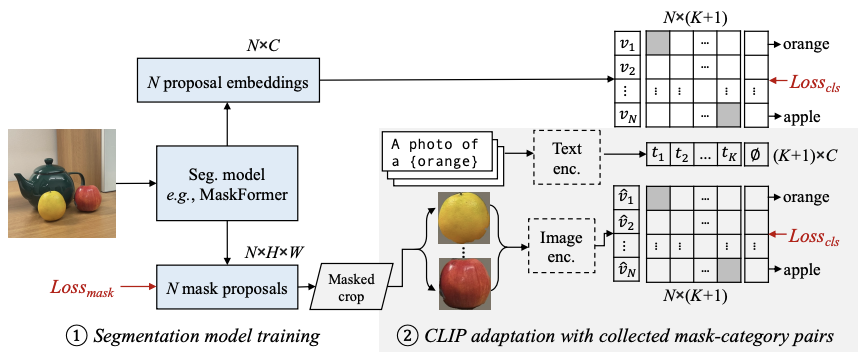
\includegraphics[width=0.48\linewidth]{figures/related_work/ovseg.png}
    }\hfill
    \subfigure[单阶段方法FC-CLIP框架图~\cite{yu2023convolutions}]{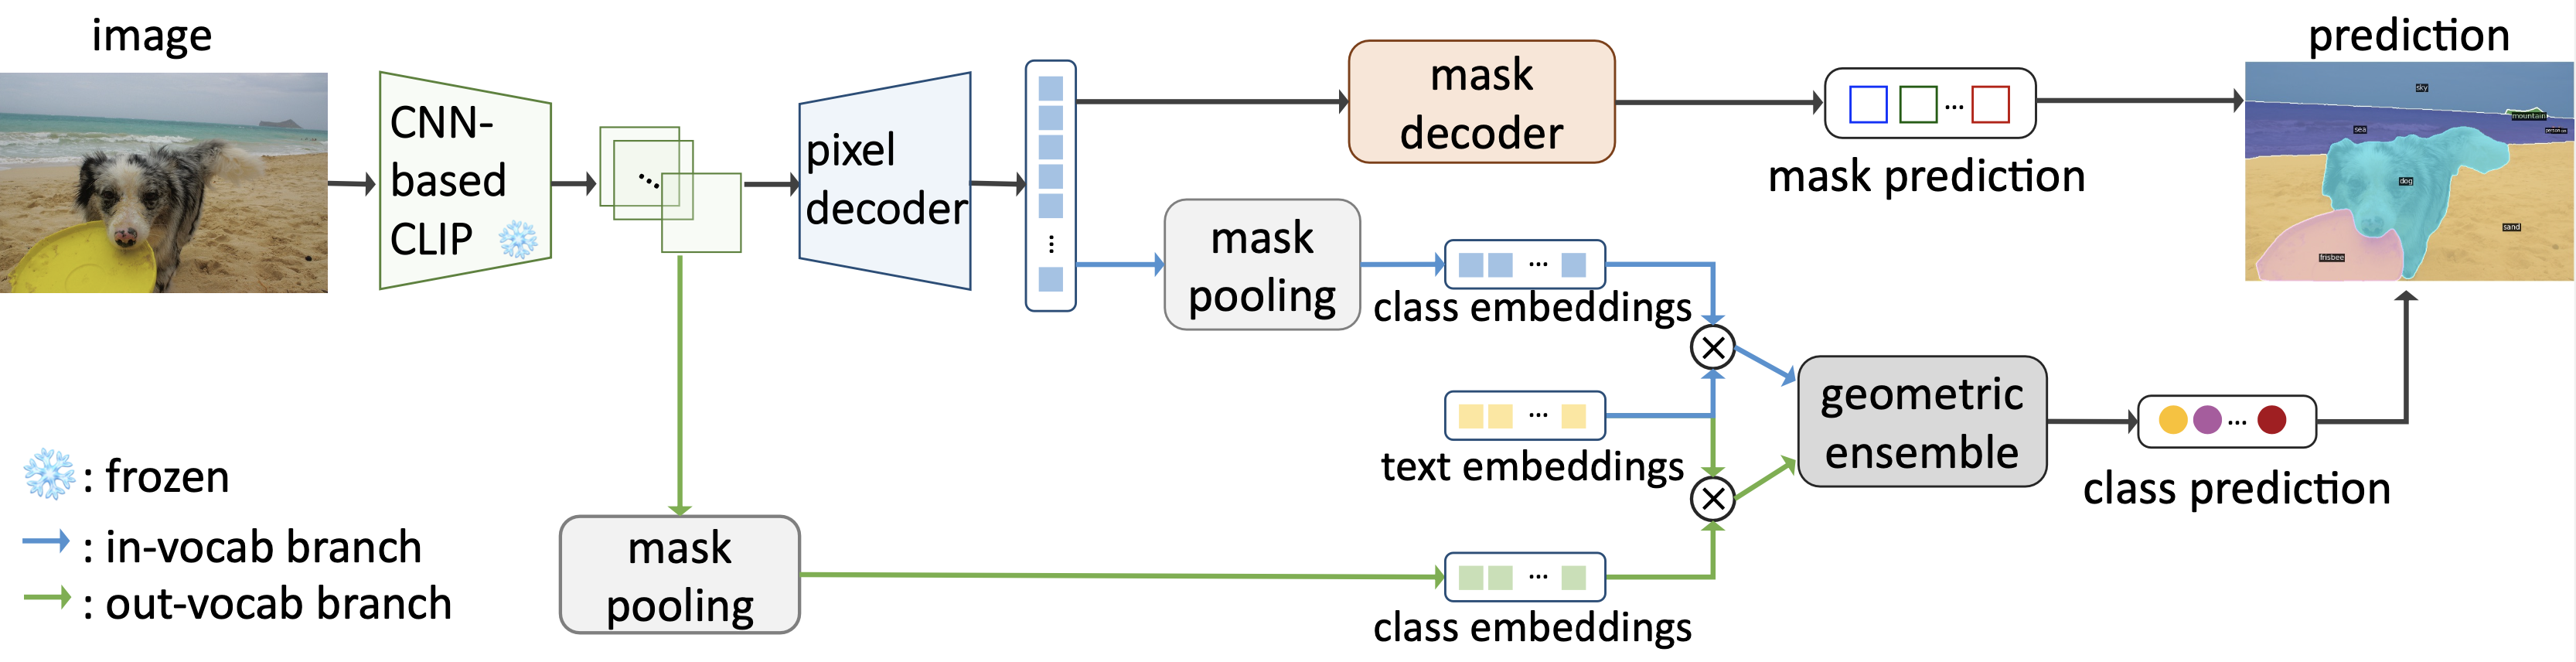
\includegraphics[width=0.48\linewidth]{figures/related_work/fc-clip.png}}
    \bicaption[fig:rare_ovs]{}{代表的开放词表方法}{Fig.}{Representative methods for open-vocabulary methods}
\end{figure}

OVS 方法可沿“先生成掩码再分类”的两阶段路径与“端到端 单阶段”两条主线展开。两阶段方法~\cite{liu2024open,maskclip,xu2022simple,MasQCLIP,liang2023open,chen2023open} 一般先借助额外分割模型生成类别无关掩码提议，再将 ViL 特征与多个掩码提议进行交互以分配语义类别。SCAN~\cite{liu2024open} 通过双流网络联合学习语义无关的掩码与类别嵌入；MaskCLIP~\cite{maskclip} 以类别无关掩码与可学习 mask token 与 CLIP 嵌入交互；OPSNet~\cite{chen2023open} 将 mask query 嵌入与 CLIP 最后一层嵌入结合用于域外类别识别， 并引入 IoU 分支过滤低质量提议；OVSeg~\cite{liang2023open} 通过在大规模开放词汇数据上微调掩码分类器提升密集预测 质量；SimBase~\cite{xu2022simple} 与 MasQCLIP~\cite{MasQCLIP} 进一步简化两阶段流水线并探索 CLIP patch 特征与掩码的对齐。 两阶段方法的主要局限是“先生成、再分类”的串行结构导致 特征不对齐与计算冗余，且对未见类别的掩码质量高度依赖 上游提议模型。

单阶段方法~\cite{yu2023convolutions,wu2024clipself,MGCCL} 将 ViL 模型本身扩展为分割器骨干，端到端地完成密集预测，避免了 掩码提议阶段带来的过拟合风险。FC-CLIP~\cite{yu2023convolutions} 通过在 CLIP 之上引入掩码分类头实现单阶段开放词汇分割； CLIPSelf~\cite{wu2024clipself} 在 CLIP 内部通过自蒸馏提升 patch 级别表征；MGCCL~\cite{MGCCL} 借助多粒度对比学习增强 文本—图像—掩码三方的语义对齐。研究表明，卷积式 CLIP 模型相较 ViT 式 CLIP~\cite{dosovitskiy2021image} 在大输入 分辨率下表现更优，这与其对空间结构的局部归纳偏置密切相关。 然而，CLIP 的 patch 级特征本质上是为图像级识别设计的， 缺乏细粒度的像素级监督，因而在 mask 边界精度与对小目标 的捕捉上存在天然上限：除像素级监督缺失外，patch 网格与对象边界之间的区域级偏置进一步削弱了掩码精度；而推理阶段文本—视觉相似度的计算开销与类别数线性相关，在开放词汇场景下还需配合高效的类别嵌入压缩。针对这些局限，现有缓解思路包括 FC-CLIP 通过卷积 CLIP 提升分辨率适应性、DenseCLIP~\cite{rao2022denseclip} 引入像素—文本密集对齐、CLIPSelf 通过自蒸馏提升 patch 级表征、MGCCL 借助多粒度对比学习联合优化。

视觉—语言基础模型与分割基础模型的融合是 OVS 突破上述困难的关键路径。CLIP 与 ALIGN 在零样本分类、检索、跨模态匹配等任务上展现强大泛化能力；SAM 凭借十亿级分割掩码训练实现任意提示引导的零样本实例分割。SAM 的适应性通过 多种提示策略进一步增强，包括低级视觉提示~\cite{MMRAD}、 弱监督~\cite{ROSE} 等；同期工作 SEEM~\cite{seem} 将空间 提示（点、框、涂鸦、掩码）与文本提示统一到联合图像—文本 表征空间；X-Decoder~\cite{zou2023seg} 通过不同 query 类型 实现任务统一。然而 SAM 本身不输出类别语义，CLIP 又缺乏 像素级密集监督，二者在统一解码框架内的深度融合仍有待 探索。RegionSpot~\cite{yang2024recognize} 通过开放词汇 检测器生成候选框并送入 SAM 完成高质量分割；Open-Vocabulary SAM~\cite{yuan2024open} 借助交互式提示在二十千类上完成 分割与识别。然而上述方法多以“检测器 + SAM”或“CLIP + 分割器” 的松耦合方式组合，掩码质量与类别语义识别之间仍存在错配： SAM 的高质量掩码与 CLIP 的开放语义难以在统一解码框架内 对齐。从松耦合到紧耦合的范式演进中，基础模型融合范式 经历了从外部检测器 + 分割器的两阶段流水线到单阶段 CLIP 骨干 + 分割头的端到端融合、再到跨模型统一解码 的演进。
% 然而上述方法均未在统一解码 框架内充分利用 SAM 的高质量掩码先验，导致掩码质量与 语义识别之间的错配。


\subsection{面向语义理解泛化场景的高阶语义评测}

上一节关注类别词表扩展后模型能否识别并定位未见类别；当目标任务进一步要求模型解释判断依据时，识别结果本身已不足以说明其语义理解是否可靠。多模态大语言模型（Multimodal Large Language Model, MLLM）能够结合图像生成开放式回答，相关评测也从对象、属性和关系的判别，逐步扩展到知识运用与解释生成。然而，答案合理或表述流畅，并不能证明解释中的语义结论得到了视觉证据支持。对这一差别的考察需要先了解通用基准如何测量感知与推理，再进入对证据依赖更强的具体任务。艺术情感理解正是此类任务的代表：情感判断往往涉及构图、色彩等多种线索，评测既要考察模型给出何种判断，也要检验其如何将判断与可见线索关联。

通用多模态基准为区分不同视觉能力提供了起点。MMBench~\cite{mmbench2023} 将感知与推理细化为多个能力维度，通过选择题比较模型在属性识别、空间关系等任务上的表现；SEED-Bench~\cite{seedbench2024} 进一步覆盖图像与视频理解，使评测对象从静态画面扩展至时间信息。ScienceQA~\cite{lu2022scienceqa} 和 MMMU~\cite{yue2024mmmu} 则将科学知识、多学科材料与图像共同纳入问答任务，提高了对知识运用和复杂推理的要求。这些基准采用不同的任务划分，它们能够揭示模型在哪类题目上答对或答错，但在以最终答案为主要评分对象时，正确答案仍不足以单独证明模型生成的解释引用了相关视觉证据。

% 图~\ref{fig:related_benchmarks} 对照展示了通用能力基准与图像情感基准的任务形式。

对开放式回答的评测进一步将注意力从答案延伸到生成内容。GAVIE~\cite{liu2024gavie} 借助模型辅助评判考察视觉指令回答的质量与幻觉；FaithScore~\cite{jing2024faithscore} 将生成描述拆解为可核验的原子事实，再检查这些事实是否与输入图像一致。前者扩展了开放回答的评判方式，后者提供了比整体流畅度更细的事实一致性度量。不过，描述中的对象和属性均属实，也不意味着模型已经说明它们为何共同支持某种抽象语义判断。面向解释本身，VQA-X~\cite{park2018multimodal} 同时收集文字理由和视觉指向，表明回答、理由及其指向的图像区域可以分别考察；其任务主要围绕视觉问答中的决策解释。


\begin{figure}[!htbp]
    \centering  
    \setlength{\tabcolsep}{0pt}
    \subfigure[视觉-语言模型多模态能力评测基准MMBench~\cite{mmbench2023}]{
        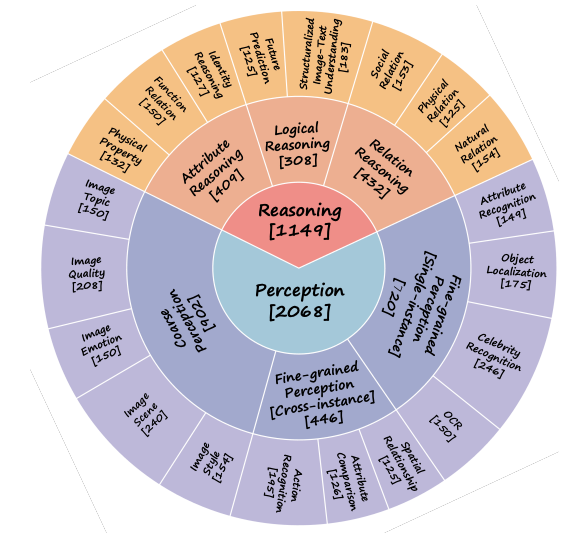
\includegraphics[width=0.48\linewidth]{figures/related_work/mmbench.png}
    }\hfill
    \subfigure[图像情感评测基准EEmo-Bench~\cite{eemobench2025}]{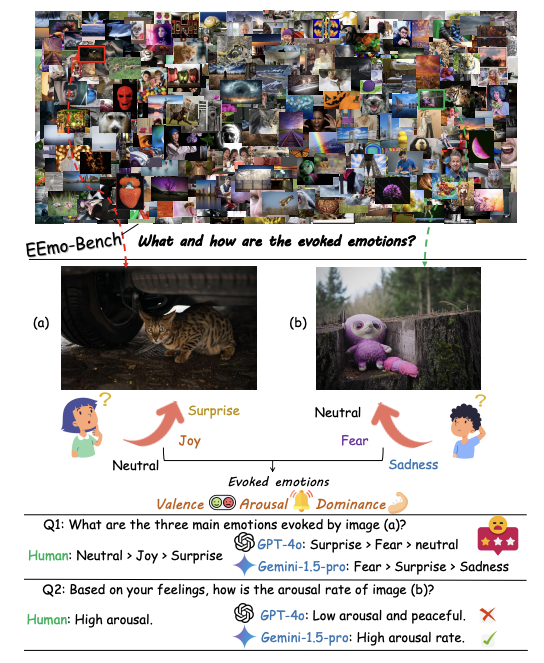
\includegraphics[width=0.38\linewidth]{figures/related_work/EEmo-Bench.png}}
    \bicaption[fig:related_benchmarks]{}{代表性的语义评测基准}{Fig.}{Representative benchmarks for semantic evaluation}
\end{figure}

艺术情感理解需要同时关注作品传达了何种情感，以及观看者依据哪些视觉线索作出判断。图~\ref{fig:related_benchmarks} 对照展示了通用能力基准与图像情感基准的任务形式。作品的情感效果可能来自对象内容，也可能来自色彩、光照、构图和笔触；不同观看者对同一作品的感受也未必一致。ArtEmis~\cite{achlioptas2021artemis} 为艺术作品收集情感归因及其文字解释，记录观看者的情感反应与理由；EmoSet~\cite{yang2023emoset} 在情感类别之外标注亮度、色彩、场景、对象、表情和动作等属性，为分析视觉内容与情感判断的关系提供了依据。效价、唤醒度与支配度等连续维度还可描述情感状态及强度差异~\cite{you2016building}。这些资源分别从解释、视觉属性和情感维度提供研究材料，但标注对象与粒度不同，尚需进一步组织为能够区分模型感知、情感判断与解释能力的评测任务。

视觉线索的定位也已有专门研究，而非完全空白。APOLO~\cite{chen2024stimuli} 将艺术作品中引发特定情感的区域标注为像素级刺激线索，使研究者能够评价模型是否找到了相关位置。这与 ArtEmis 的自然语言解释形成互补：前者强调证据位于何处，后者记录观看者如何表述感受及其理由。但定位到某个区域，并不能自动判断模型是否正确解释了该区域的形式属性与情感含义之间的关系；反过来，一段合理的文字解释也未必精确指向相关视觉区域。因此，情感归因需要同时关注线索识别、语义关联与解释质量。

在上述情感标注与视觉线索研究的基础上，面向 MLLM 的工作进一步将情感理解组织为可比较的评测任务。EEmo-Bench~\cite{eemobench2025} 涵盖单图感知、情感排序、描述与评估，并通过配对图像考察模型对情感差异的辨别能力，表明单一分类准确率不足以概括情感理解水平。相邻的美学评测研究也逐步引入细粒度属性与开放式描述：AesExpert~\cite{aesexpert2024} 构建多类型美学评价指令，ArtiMuse~\cite{cao2025artimuse} 结合属性分析、专家式评述与整体评分。不过，美学质量评价与情感归因的目标并不相同；即使模型能够给出合理的情感描述，仍需进一步判断其解释是否准确关联了作品中的具体视觉线索。

综上，已有研究分别推进了通用问答、事实一致性、视觉指向、情感标注和美学评论的评测。真正需要进一步衔接的是三种可区分的判断：模型是否识别了作品中的相关线索，能否据此作出情感判断，以及能否在解释中准确建立线索与判断的联系。仅比较最终情感标签、文字流畅度或证据区域，均难以单独定位这一链条中的失效环节。本文在第五章以艺术情感推理为目标任务，将感知、情感、推理和描述设计为相互补充的评测维度，结合单图与配对任务刻画 MLLM 既有能力向高阶语义任务延伸时的适用范围；评测旨在诊断能力边界，而非通过评测本身提升模型性能。

\subsection{现有方法的主要问题}

\noindent\textbf{（1）现有无监督方法在跨域分布偏移下的不确定性建模上存在瓶颈}

无标签目标域中的迁移不确定性同时涉及目标预测的可靠性和特征表征的稳定性。现有伪标签自训练方法往往依据预测置信度或固定阈值筛选样本；当源模型在目标域发生系统性偏移时，高置信预测也可能出错，筛选结果因而难以准确反映伪标签的可靠程度。另一方面，骨干网络可能保留源域纹理、背景或空间共现等域特异性线索，使目标特征的类别结构发生偏移，并进一步影响伪标签生成。两类问题在迭代训练中相互作用：不稳定的表征增加错误伪标签，错误监督又可能强化原有的特征偏移。因此，现有方法仍需解决如何在不访问源数据的条件下评估目标样本的监督可靠性，并同时抑制骨干表征中的虚假相关性，以减轻自训练过程中的误差累积。

\noindent\textbf{（2）现有少监督方法在信息驱动的样本挖掘与跨模态协同上存在不足}

在目标域仅有少量标注样本可用的稀缺监督条件下，如何拓展监督信号的来源与协同深度，是模型迁移设定下的另一关键研究问题。视觉—语言等大模型凭借大规模跨模态预训练获得了对开放语义的零样本判别能力，其预测不依赖源域分布，能够为目标样本提供与源模型假设空间互补的语义判断信号，这对缓解源模型在目标域上的预测偏置、扩展稀缺标注预算下的监督信息量具有重要价值。然而现有方法在样本选择与跨模态协同两个环节均缺乏对多模态预训练模型监督信号的系统探索，未能建立视觉—语言模型与源模型在信息驱动采样与双向深度协同层面的严谨理论框架。因此，如何实现视觉—语言模型与源模型在信息驱动采样与双向深度协同层面的协同，是模型迁移研究需要解决的关键问题。

\noindent\textbf{（3）现有跨类泛化方法在多流语义对齐与空间定位上探索不足}

视觉—语言模型与分割基础模型分别提供了开放词表的语义锚点与像素级空间定位能力，二者的协同融合被视为突破该问题的关键路径。然而现有方法在多流语义对齐与空间定位两个层面均存在不足：在多流语义对齐层面，两阶段与单阶段方案均难以在统一框架下实现掩码生成与开放词汇识别之间的深度协同；在空间定位层面，现有方案难以同时兼顾对像素级对齐的精细建模与对未见类别的掩码质量，致使对长尾与未见类别的细粒度识别能力受限。因此，如何在统一解码框架内深度融合分割基础模型的空间定位能力与视觉—语言模型的开放词汇语义能力，通过多流语义对齐与空间定位的协同优化实现对长尾与未见类别的泛化，是跨类泛化研究亟待解决的核心问题。

\noindent\textbf{（4）现有语义理解基准在证据锚定与评测维度建模上存在缺口}

语义理解要求模型在开放式语义理解的基础上具备对抽象语义与文化背景的稳健推理能力。语义类评测相对事实类评测具有显著的特殊性：受主观性、抽象性与文化语境三重影响，语义类内容的可靠解释难以被“事实正确性”或“流畅表述”等单一维度度量。已有研究分别提供了情感解释文本、视觉刺激区域、多维情感任务和美学属性分析，但这些评测对象尚未充分贯通，因而难以区分模型是遗漏了相关线索、错误地建立了线索与情感的关联，还是仅在文字表述上缺乏证据支撑。因此，如何构建兼具结构化诊断能力与开放式评分灵活性的多层级评测基准，是语义理解评测需要进一步解决的问题。

\section{本文的主要研究内容及组织结构}

\subsection{本文的研究内容}

前文表明，训练与目标条件之间的差异既可能改变样本分布和类别范围，也可能提高目标任务对语义解释的要求。针对数据分布与类别词表变化，本文研究如何利用有限的目标侧信息和预训练先验改善模型的迁移表现；针对语义理解要求的提高，本文研究如何在不更新模型的条件下评估既有能力的适用范围。两类工作分别从能力提升和能力评测回应多泛化场景下的模型迁移问题，具体归纳为以下四个研究问题。


\noindent\textbf{（1）无监督模型迁移的不确定性抑制问题}

无监督模型迁移中的不确定性源于源模型所学判别依据与目标域数据之间的失配，并在伪标签自训练过程中持续演化：域特异性线索使目标表征和预测偏移，错误预测被赋予伪标签后又作为监督信号参与更新，进一步放大初始偏差。本文围绕这一不确定性的产生、估计与传播开展研究。首先，以目标样本的邻域结构估计伪标签可靠性，识别并抑制错误监督在判别层的累积；其次，考察骨干网络对跨通道关系和背景空间共现的建模方式，削弱域特异性虚假相关对表征及后续伪标签生成的影响。由此，本文将可靠监督信号的构建与跨域稳定表征的学习联系起来，研究二者如何共同抑制无标签适应过程中的误差反馈。

\noindent\textbf{（2）少监督模型迁移的信息最大化问题}

在目标域标注稀缺的条件下，少监督模型迁移需要解决的核心问题是：有限的监督信息能否有效约束目标域中的预测误差，使模型在分布偏移下仍获得可靠的判别能力。这里的信息最大化是固定监督预算下提高目标域学习收益的研究目标。现有方法分别从标注样本利用和目标模型训练等角度提高迁移性能，但对有限监督如何覆盖目标域差异、如何转化为目标模型能力仍缺乏统一刻画。本文据此分析标注集合的覆盖缺额及补充监督与目标模型之间的差异，并进一步研究主动样本选择和跨模型协同学习，使有限标注与互补语义知识共同改善目标域预测。

\noindent\textbf{（3）模型泛化的多模态类别先验挖掘问题}

跨类泛化的核心要求是模型对训练阶段未见过的新颖类别保持识别能力，其关键在于系统挖掘并融合多源类别先验。现有方法多沿单一先验源或粗粒度拼接展开，缺乏在不同网络层级上的双向注入与协同机制。本文从多层级协同融合与双向耦合两个维度展开：在多层级协同融合层面，使空间定位与开放词汇语义两类先验在不同网络深度上交叉作用而非简单串接；在双向耦合层面，使两类先验在网络前向推理中相互增强而非单向辅助，从而在多个细粒度识别任务上取得优于现有方法的性能。

\noindent\textbf{（4）多维度语义理解基准制定问题}

现有评测已分别涉及情感标签、视觉属性、解释文本与刺激区域，但缺少在同一任务体系中追踪感知线索、情感判断及证据化解释之间关系的诊断方式。本文围绕证据化解释与多维度诊断两个要素展开：在证据化解释层面，区分有视觉依据的情感解释与缺乏相关依据的流畅表述；在多维度诊断层面，将语义理解能力拆解为互补任务，并结合结构化题目与开放式评分定位具体能力缺口。

\subsection{本文的组织结构}

\begin{figure}[!htbp]
 \centering
 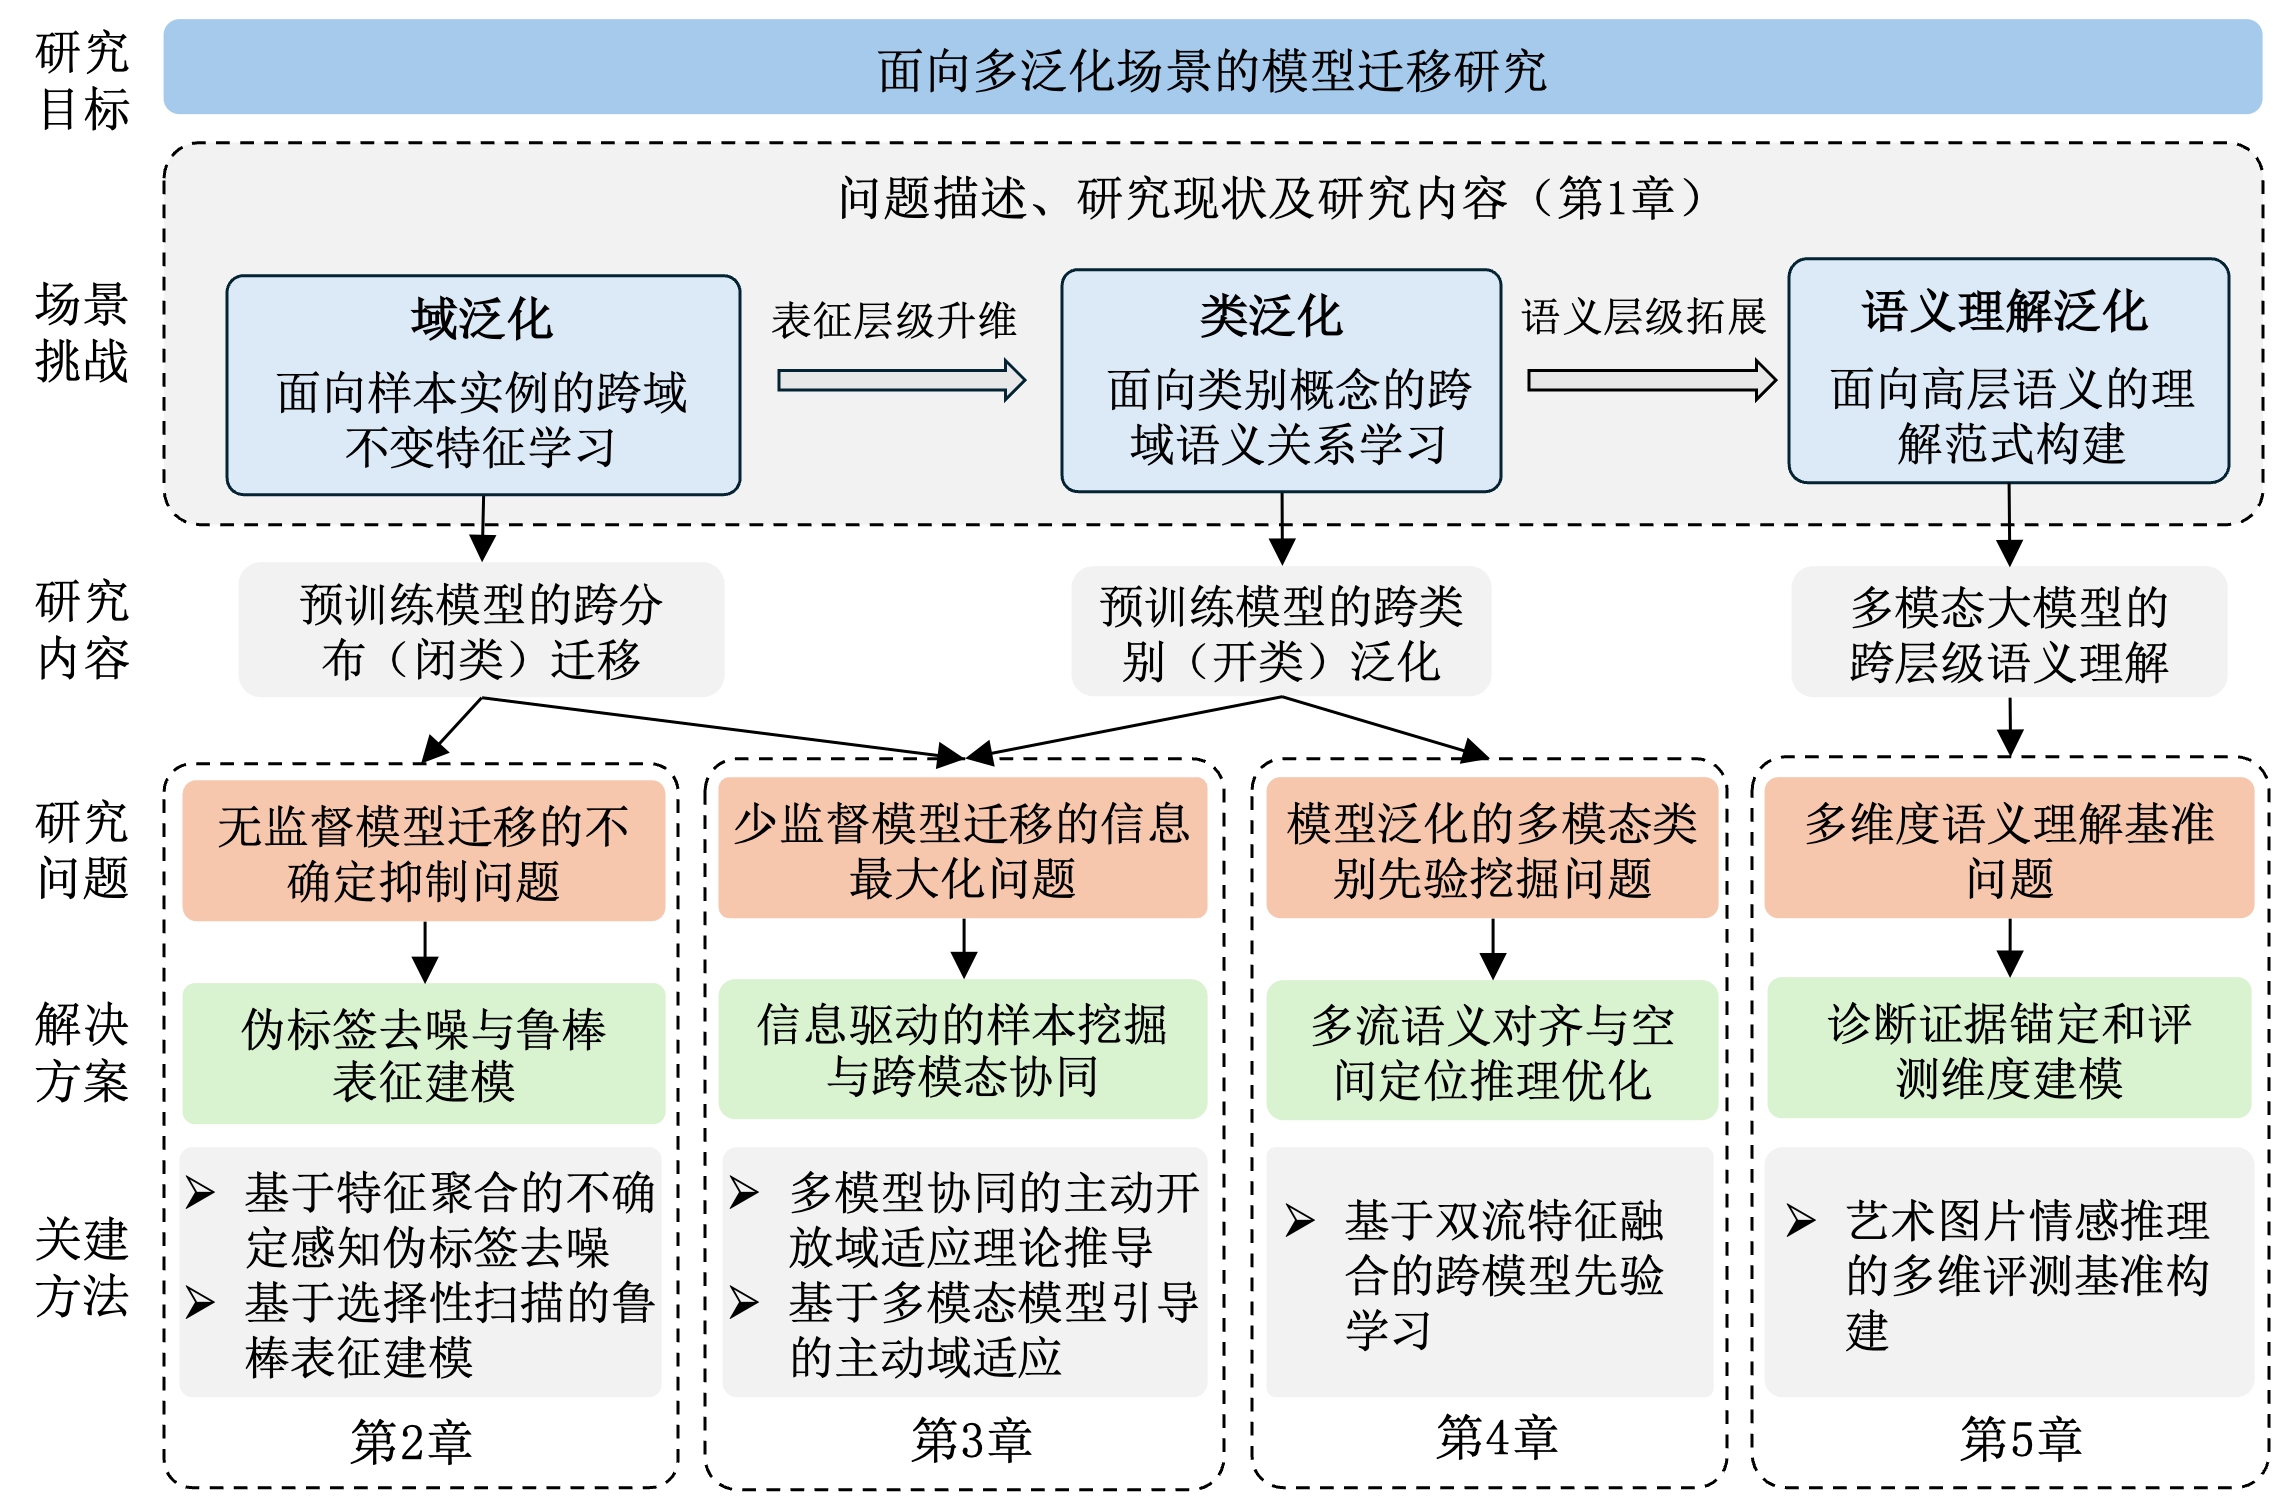
\includegraphics[width=1.\textwidth]{figures/frame.png}
 \bicaption[fig:research_map]{}{面向多泛化场景的模型迁移研究框架}{Fig.}{Research framework of model transfer across multiple generalization scenarios.}
\end{figure}


本文的研究目标是面向多泛化场景的模型迁移研究。如图~\ref{fig:research_map}所示，本文以数据分布、类别词表和语义层次的变化为主线，将研究内容组织为域泛化、类泛化和语义理解泛化三个递进层次。三个层次分别对应预训练模型的跨分布闭类迁移、跨类别开类泛化，以及多模态大语言模型的跨层级语义理解。
% 本文主要研究内容及各章节关系如图~\ref{fig:research_map}所示。

首先，本文面向样本实例的跨域不变特征学习，研究无监督模型迁移中的不确定性抑制问题。无源域适应中，源模型对域特异性线索的依赖可能使目标域表征与预测发生偏移；由此产生的错误伪标签又会在自训练中传播，进一步放大迁移误差。针对伪标签监督的可靠性问题，本文提出基于特征聚合的不确定性感知伪标签去噪方法 UPA，利用邻域一致性估计样本级伪标签可靠性，并结合类别感知对比学习抑制噪声传播；针对表征建模中的虚假相关性问题，提出基于选择性扫描的迁移方法 SfMamba，通过通道级视觉状态空间模块与语义一致性打乱策略增强跨域表征的稳定性。两项工作分别作用于监督信号和特征表征环节，在统一自训练框架下共同减轻迁移误差的累积。
在此基础上，面向稀缺标注预算下跨模型协同监督不足的问题，针对源模型与视觉—语言模型假设空间层面的信息对齐与知识迁移问题，提出基于多模态基础模型引导的双主动域适应方法 DAMF，将视觉—语言模型作为目标样本与源假设空间之间的互补语义监督信号，通过双聚焦样本选择与交替蒸馏实现两类模型在开放集假设空间的双向深度协同。

面向跨类泛化这种面向类别概念的跨语义关系学习，首先针对开放集无源域适应中已知类别与未知类别难以同时兼顾的问题，利用视觉—语言模型在自然语言空间的零样本识别能力指导目标域已知类的判别建模，进一步通过不确定性感知的开放集校准机制实现对未知类别样本的可靠识别；其次针对开放词汇分割中掩码质量与类别语义识别之间的错配问题，视觉定位模型擅长像素级定位但缺乏语义泛化能力、语义—语言模型具备零样本识别能力但特征空间偏全局且边界粗糙，提出跨模型先验融合的开放词汇分割方法 CMPF，将定位模型的空间先验与语义模型的类别先验在统一解码框架内交叉融合，实现对未见类别的稳定识别。

进一步的，面向多模态多维度的情感评测的基准构建需求，针对多维度语义理解基准制定问题，构建AER-Bench，建立从低层视觉线索到高层情感推理的结构化诊断框架，将艺术情感理解拆解为感知维度、情感与 VAD、基于证据的推理、情感描述四个互补层级并模板化生成单图/配对结构化题目，通过确定性指标与基于大语言模型的细粒度评分相结合的混合协议，对代表性多模态大语言模型在艺术情感推理上的能力进行系统评测，揭示其在视觉证据锚定、感知—情感映射与情感解释一致性上的系统性缺陷。

相关研究沿图~\ref{fig:research_map}所示的表征层级升维与语义层级拓展展开：前两层以适应方法提升跨分布与跨类别能力，第三层以多维评测刻画跨层级语义理解的能力边界，共同构成本文对多泛化场景下模型迁移的研究。
% Local Variables:
% TeX-master: "../thesis"
% TeX-engine: xetex
% End:

% !Mode:: "TeX:UTF-8"

\chapter[基于特征聚合与选择性扫描的无监督域迁移]{基于特征聚合与选择性扫描的无监督域迁移}[]
\chaptermark{基于特征聚合与选择性扫描的无监督域迁移}

\label{chap:2}

% 图表与公式编号按章重置并显示为 "章-序"（X-Y）格式，
% 由 book.cls 的 \newcounter{figure}[chapter] / \@addtoreset{equation}{chapter}
% 与 hithesisbook.cls 的 \thefigure / \thetable 定义共同保证；
% 此处不可再调用 \counterwithin，它会把编号改写为 "X.Y" 且全局泄漏到后续章节。

\section{引言}

跨数据域分布偏移是模型迁移学习面临的核心挑战之一。由于源域与目标域在成像条件、视觉风格、背景结构和样本统计特性等方面存在差异，模型在源域中学习到的判别规则往往难以直接适用于目标域。当目标侧缺乏可靠监督信号时，模型只能依赖自身预测或结构先验完成适应，迁移误差便容易在训练过程中持续累积。如何在分布变化和监督缺失的双重约束下获得可靠的目标域模型，是跨域迁移研究需要解决的关键问题。
在数据隐私、存储成本和商业机密等现实约束下，源域样本通常无法在目标域适应阶段持续访问。与可同时使用源域和目标域数据的传统域适应方法相比，无源域适应（Source-Free Domain Adaptation, SFDA）仅保留预训练源模型，在不访问源域样本的条件下将其迁移至无标签目标域。此时，源样本重构、显式源—目标分布对齐和域判别等常用机制均难以直接采用，模型需要完全依赖目标域数据及源模型所携带的知识完成适应，因而进一步放大了迁移过程中的不确定性。

这种不确定性主要体现为两个相互耦合的层面。其一，骨干网络提取的表征能否在跨域后保持稳定的判别结构，决定了目标样本在特征空间中的可分性；其二，伪标签能否提供可靠监督，决定了自训练过程是否会朝正确方向更新。表征质量不足会降低伪标签可靠性，而错误伪标签又会通过迭代优化持续损害特征表征，形成表征退化与监督噪声相互强化的闭环。因此，可靠的无源域适应不仅需要抑制伪标签噪声，也需要增强跨域表征的鲁棒性。


作为跨域迁移伪标签自训练的主流技术路线之一，源假设迁移（Source-Hypothesis Transfer, SHOT）~\cite{liang2021source}提出的伪标签自训练框架已被广泛采纳并衍生出大量改进工作~\cite{fan2021dda,wang2025osda}，其基本流程可概括为三步：冻结源域分类器，以源模型对目标样本的初始预测为锚点进行聚类生成伪标签；以伪标签为监督信号并叠加信息最大化（Information Maximization, IM）~\cite{gomes2010discriminative}损失对特征提取器进行更新；通过迭代聚类—更新循环逐步精炼伪标签质量。然而，该框架的效果仍受限于特征表征和伪标签监督之间的耦合关系：当骨干网络缺乏对跨域稳定语义的有效建模时，聚类结果易受域特异性因素干扰；当伪标签包含噪声时，自训练又会放大错误监督，进而限制模型性能。

针对上述问题，本章将源—目标域差异引发的表征退化、伪标签噪声统一视为迁移不确定性的不同表现，并按不确定性的归属层次组织研究工作。
判别层的不确定性表现为伪标签噪声：只要基于聚类生成的伪标签发生错误分配，噪声就会通过自训练回路在判别层累积传播。
% 并沿卷积神经网络CNN与状态空间模型（State-Space Model, SSM）两条骨干路径开展研究。面向CNN 骨干，
针对该层次，本章提出基于特征聚合的不确定性感知伪标签去噪方法 UPA，借助特征空间邻居一致性估计样本级不确定性以自适应筛选高质量伪标签，并通过类感知对比学习阻断残余噪声的记忆传播，从去噪与对比正则两个角度抑制跨域迁移过程中判别层的不确定性传播。
表征层不确定性则与骨干的建模方式直接相关：状态空间模型以选择性扫描展开空间序列，其跨通道频率域依赖建模不足，且隐藏状态演化会记忆源域中前景与背景的空间共现模式。为此，本章在判别层去噪机制的基础上进一步提出基于选择性扫描的不确定性感知迁移方法 SfMamba，针对上述两类骨干相关的不确定性，通过通道级视觉状态空间模块显式建模跨通道频率域依赖以稳定源域表征，通过语义一致性打乱策略在自训练阶段主动扰乱背景 patch 的空间共现以阻断序列层虚假相关性的累积，以线性复杂度实现高效长程跨域建模。SfMamba 在状态空间骨干上沿用 UPA 的邻居感知去噪机制，使判别层去噪与骨干级增强在同一自训练框架中协同发挥作用。

本章在 Office、Office-Home、VisDA-C 和 DomainNet-126 四个 SFDA 基准上开展实验，验证所提方法在不同跨域任务中的有效性，并分析其在适应精度与计算效率之间的权衡。

本章工作可归纳为以下三点：
\begin{enumerate}
    \item 判别层不确定性抑制：提出基于特征空间邻居一致性的样本级不确定性估计方法与类感知对比学习策略，从去噪与对比正则两个角度协同抑制噪声标签的记忆传播。
    \item 表征层不确定性抑制：针对状态空间骨干在跨域迁移中特有的通道建模缺失与空间序列虚假相关性累积问题，分别设计通道级视觉状态空间模块与语义一致性打乱策略，在通用去噪组件之上形成骨干级增强。
    \item 在四个基准数据集上验证上述不确定性分层抑制机制的有效性，优于其他基线方法。
\end{enumerate}


\section{基于特征聚合的不确定性感知伪标签去噪方法}

\label{sec:chap2_upa}

本章两条方法均建立在统一的 SFDA 任务设定之上：给定带标签源域数据 $\mathcal{S} = \{(x_i^s, y_i^s)\}_{i=1}^{n_s}$ 与无标签目标域数据 $\mathcal{T} = \{x_i^t\}_{i=1}^{n_t}$，两者共享标签空间 $\mathcal{Y}$，且 $|\mathcal{Y}| = C$。源域与目标域的边缘分布存在差异，即 $Q(x) \neq P(x)$，但条件分布保持一致：$Q(y \mid x) = P(y \mid x)$。源域模型 $\theta_s = f \circ g$ 在源域数据 $\mathcal{S}$ 上完成预训练，其中 $g: \mathcal{X} \to \mathbb{R}^D$ 为特征提取器，$f: \mathbb{R}^D \to \mathbb{R}^C$ 为分类器。目标域适应阶段，源域数据 $\mathcal{S}$ 不可访问；目标模型 $\theta_t$ 以 $\theta_s$ 为初始化，仅通过目标域无标签数据进行自训练。本章两条方法均遵循以下基本设定：分类器 $f$ 在适应阶段保持冻结以提供稳定的任务锚点，仅对特征提取器 $g$ 进行更新，避免源域知识的灾难性遗忘。

两类方法均建立在 SHOT~\cite{liang2021source} 提出的伪标签自训练框架之上：首先利用源域模型的初始预测对目标域样本进行聚类，生成伪标签；随后采用信息最大化（IM）损失~\cite{gomes2010discriminative} 和伪标签监督损失对 $g$ 进行更新。SHOT 的局限在于：其通过伪标签噪声传播的累积误差对骨干架构的选择较为敏感，且CNN 骨干的局部感受野不足以捕获跨域不变的长程特征依赖。本章的 UPA 与 SfMamba 分别从判别层去噪与表征—序列双层增强两个角度改进该框架，统一体现为对迁移不确定性的抑制。具体地，设当前模型对目标样本 $x^t$ 的预测概率分布为 $p(x^t) = \delta(\theta_t(x^t))$（$\delta$为Softmax函数），按 SHOT 范式进行迭代聚类：
\begin{equation}
\boldsymbol{\mu}^{(k)}_c = \frac{\sum_{x^t \in \mathcal{T}} \mathbf{1}(\hat{y}^{(k)}_t = c) \, g(x^t)}{\sum_{x^t \in \mathcal{T}} \mathbf{1}(\hat{y}^{(k)}_t = c)}, \qquad
\hat{y}^{(k+1)}_t = \arg\max_c \, d\!\left(g(x^t), \boldsymbol{\mu}^{(k)}_c\right),
\label{eq:chap2_proto}
\end{equation}
其中 $d(\cdot, \cdot)$ 为余弦相似度，$\mathbf{1}(\cdot)$ 为指示函数。经验上两轮迭代即可收敛，记最终伪标签为 $\hat{y}_t$。借鉴 IM 损失，对模型预测熵最小化来鼓励对单样本给出确定性预测，并且使用多样性正则化来防止预测集中于少数类别：
\begin{equation}
\mathcal{L}_{\text{IM}} = \mathcal{L}_{\text{ent}} + \mathcal{L}_{\text{div}}, \quad
\mathcal{L}_{\text{ent}} = -\mathbb{E}_{x^t} \sum_c p_c(x^t) \log p_c(x^t), \quad
\mathcal{L}_{\text{div}} = \sum_c \hat{p}_c \log \hat{p}_c,
\label{eq:chap2_im}
\end{equation}
其中 $\hat{p} = \mathbb{E}_{x^t}[p(x^t)]$ 为平均预测分布。$\mathcal{L}_{\text{div}}$ 通过惩罚 $\hat{p}$ 偏离均匀分布 $1/C$ 来促进类别平衡。

判别层是伪标签自训练范式中迁移不确定性的主要载体。骨干结构会影响这一噪声的严重程度。以 CNN 为例，其特征空间虽具备层次化聚合能力，但固定局部感受野对跨域长程依赖建模不足，使得基于聚类得到的伪标签不可避免地包含错误分配，而噪声的载体始终是判别层的伪标签本身。
这些错误标签通过自训练回路在判别层累积传播，构成 CNN 骨干路径上迁移不确定性的核心来源。UPA 的核心动机来自一个关键实验观察：在 VisDA-C 数据集上，若人工剔除 SHOT 生成的错误伪标签（SHOT-clean），适应精度从 82.9\% 显著提升至 88.4\%（图~\ref{fig:motivation_shot}），揭示自训练范式的性能上限很大程度上被判别层伪标签噪声所限制。现有判别层去噪方法依赖额外的辅助模型，例如双分类器~\cite{liang2021source}、动量平均模型~\cite{tarvainen2017mean} 等，来估计不确定性，但额外模型的预测偏差会引入新的建模误差。UPA 的关键观察是：在 CNN 特征空间中，正确伪标签对应的样本聚集紧密形成清晰类别簇，而错误伪标签对应的样本散布于类别边界或簇间区域（图~\ref{fig:feat_cluster}），这一聚类结构差异使得邻居分布成为无需额外模型的样本级不确定性估计来源。基于此，UPA 提出了由粗到精的二阶段去噪流水线，如图~\ref{fig:framework}所示：第一阶段通过自适应伪标签选择模块基于特征空间邻居一致性将目标域样本划分为干净集 $\mathcal{T}_c$ 与噪声集；第二阶段通过类感知对比学习策略在干净集上实施类别级对比学习，阻断残余噪声在表征空间的记忆传播。两阶段共同实现对判别层迁移不确定性的由粗到精抑制。

\begin{figure}[!htbp]
    \centering
    \setlength{\tabcolsep}{0pt}
    \subfigure[]{%
      \includegraphics[width=0.48\linewidth]{papers/UPA/fig_1_v3.pdf}
      \label{fig:motivation_shot}%
    }\hfill
    \subfigure[]{%
      \includegraphics[width=0.48\linewidth]{papers/UPA/re-fig1_2.pdf}
      \label{fig:feat_cluster}%
    }
    \bicaption[fig:upa_motivation]{}{UPA 的两个动机观察}{Fig.}{Two motivation observations of UPA}
\end{figure}

\begin{figure*}[!htbp]
  \centering
  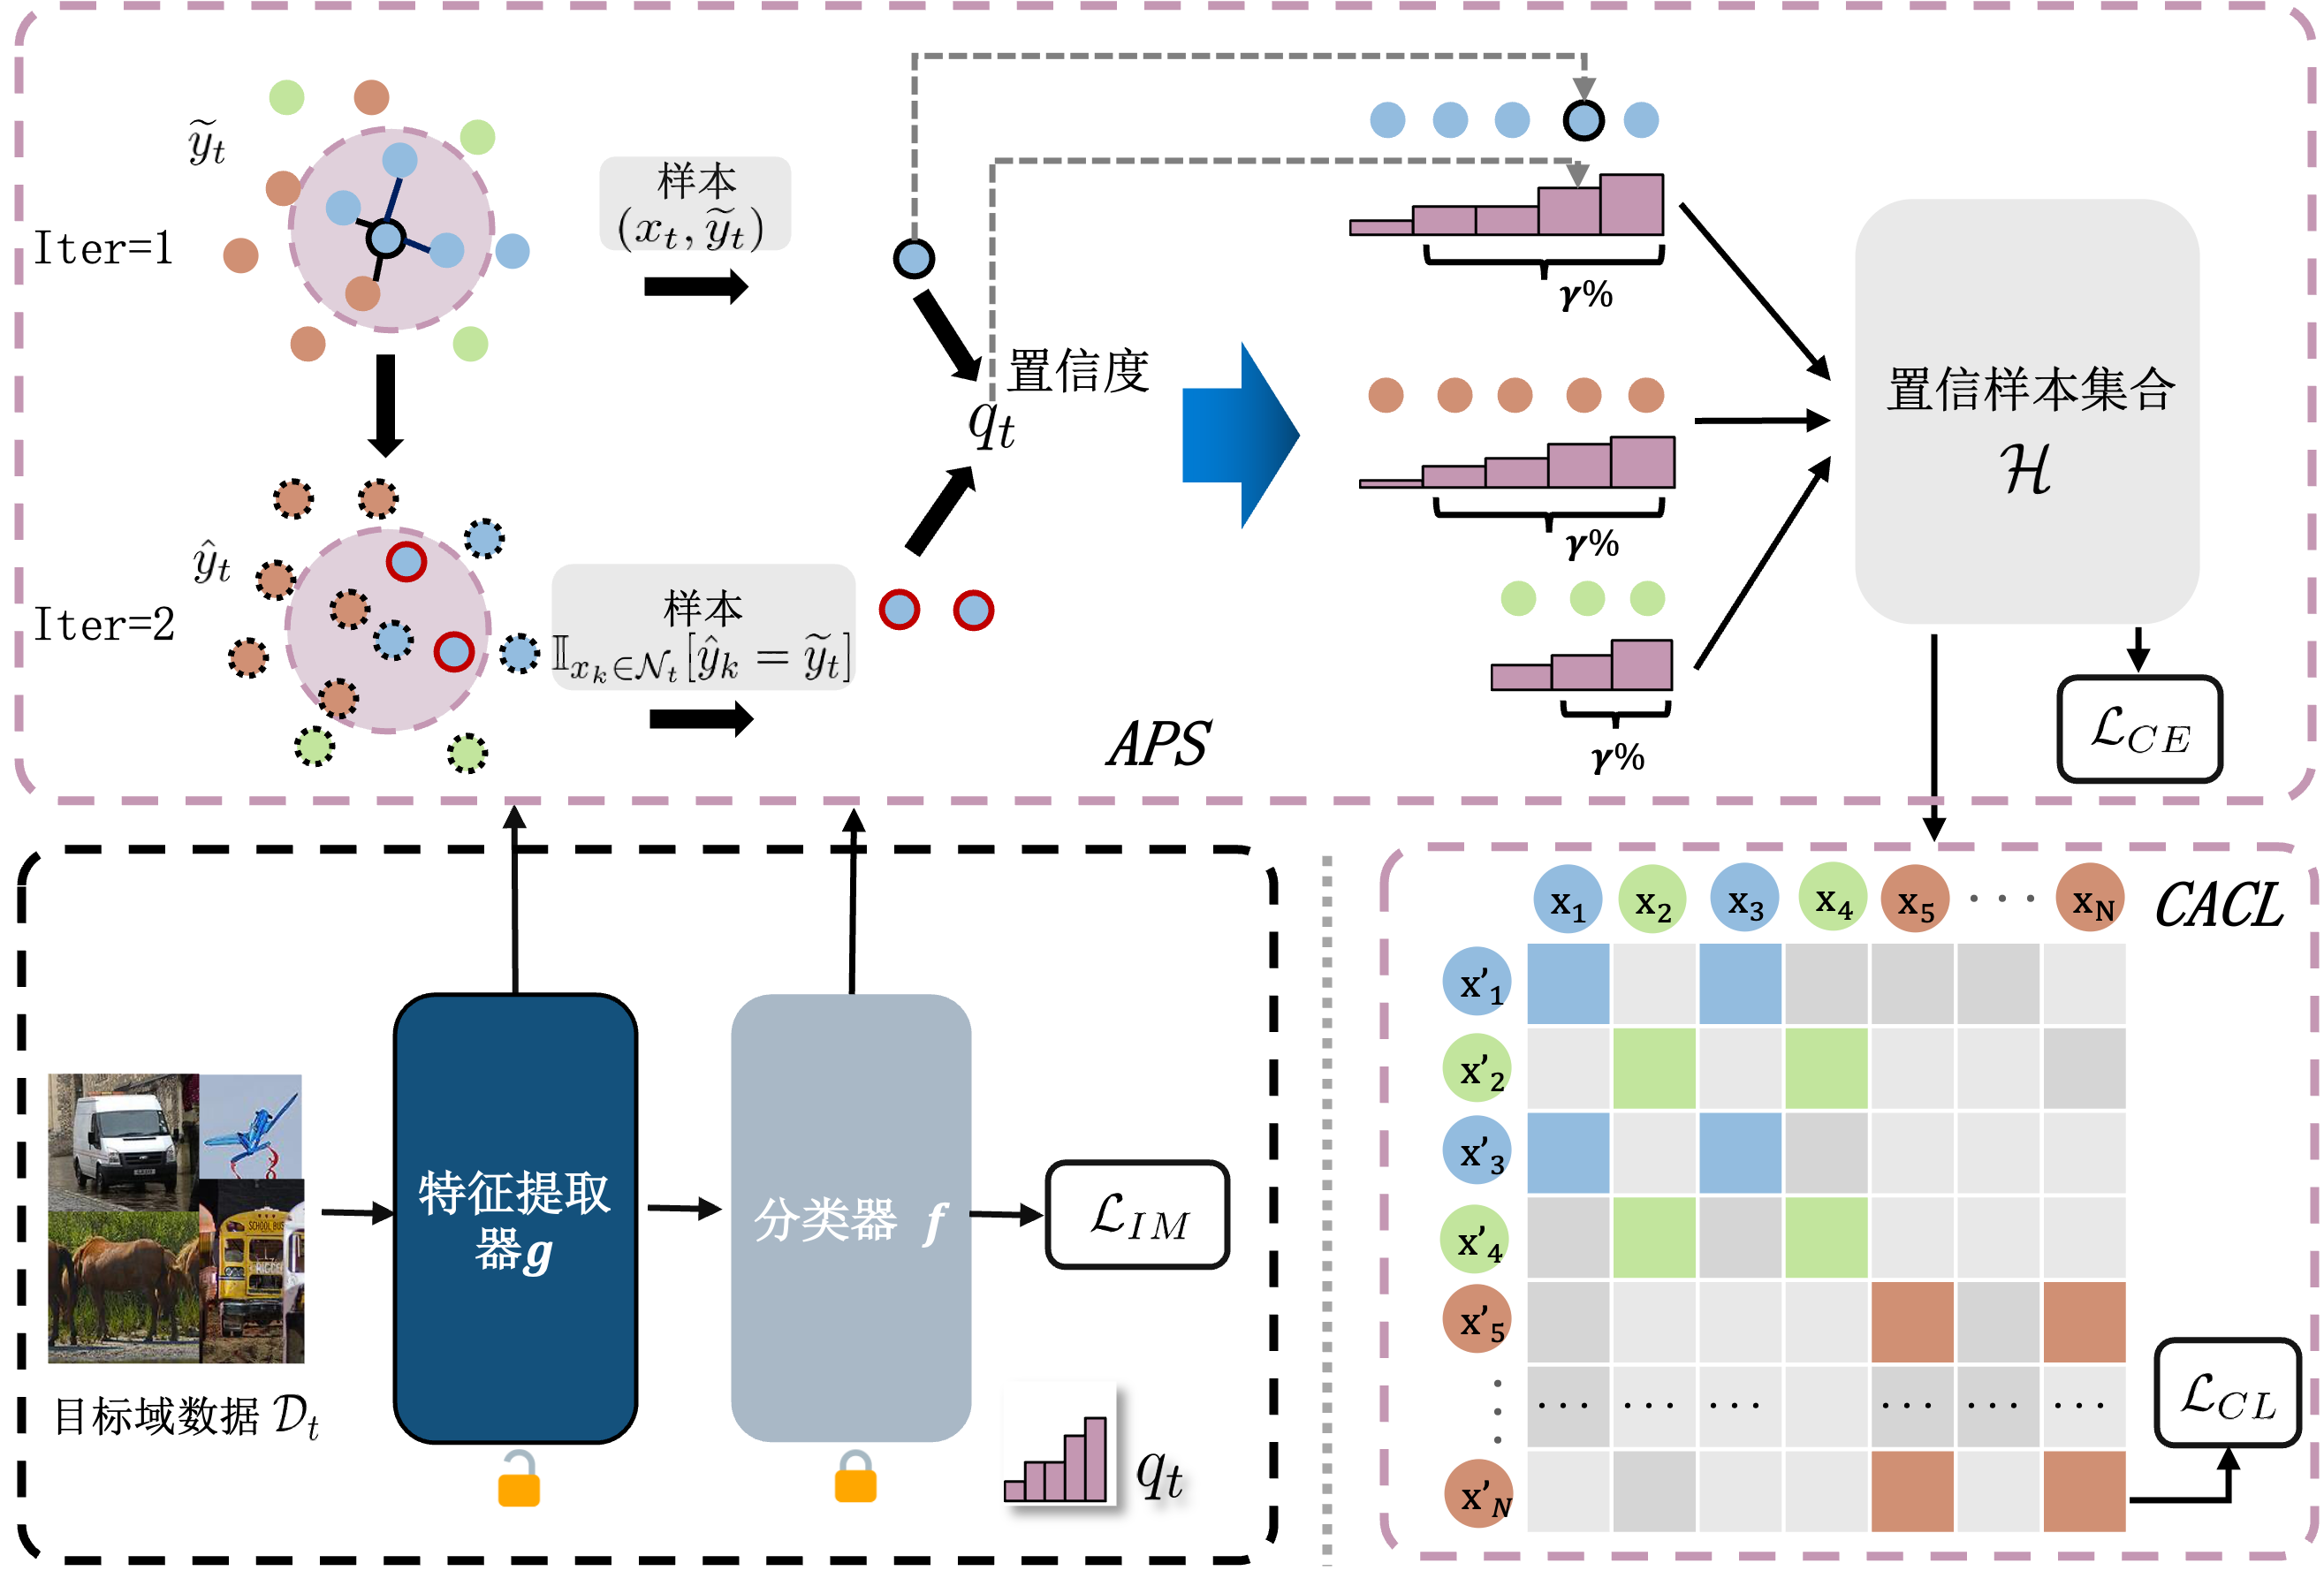
\includegraphics[width=0.85\textwidth]{figures/upa_extracted/v6_framework.png}
  \bicaption[fig:framework]{}{UPA 方法整体框架}{Fig.}{Overall framework of UPA.}
\end{figure*}

\subsection{邻域一致性驱动的判别层去噪}

\label{sec:chap2_upa_denoising}

我们假设：在特征空间 $g(x_t)$ 中，那些易于聚类的样本因同一类别内存在相似特征而包含更高程度的域共享信息；相比之下，大量不确定样本则分布在聚类中心之间，这主要源于域间的分布偏移。受此启发，我们提出了一种新颖的伪标签去噪机制 APS，该机制通过近邻样本来迭代评估样本的不确定性：

对所有目标样本的特征向量 $\ell_2$ 归一化后，计算两两余弦相似度构成相似度矩阵 $\mathbf{S}_t \in \mathbb{R}^{n_t \times n_t}$。对每个样本 $x_t$，取相似度最高的 $K$ 个样本（不含自身）作为其 K 近邻集合 $\mathcal{N}_t$。

APS 通过邻居集合进行距离加权投票，估计样本 $x_t$ 的类别后验概率 $\hat{p}_t \in \mathbb{R}^C$：

\begin{equation}
\hat{p}_t = \frac{1}{K} \sum_{x_k \in \mathcal{N}_t} d\!\left(g(x_t), g(x_k)\right) e_{\hat{y}_k},
\label{eq:knn_voting}
\end{equation}
其中 $e_{\hat{y}_k} \in \mathbb{R}^C$ 为伪标签 $\hat{y}_k$ 的 one-hot 向量。临时伪标签通过下式更新：
\begin{equation}
\hat{y}_t = \arg\max_c \, \hat{p}_t^{(c)}.
\label{eq:label_update}
\end{equation}

实验验证，两轮迭代即可收敛。该估计过程完全发生在特征空间内部，无需任何额外模型，符合特征空间自洽性的核心命题。
在不确定性估计完成后，本文用置信度评分 $q_t$ 来量化伪标签质量：
\begin{equation}
q_t = \frac{1}{K} \sum_{x_k \in \mathcal{N}_t} \mathbf{1}\!\left(\hat{y}_k = \hat{y}_t\right) d\!\left(g(x_t), g(x_k)\right).
\label{eq:confidence}
\end{equation}
$q_t$如图~\ref{fig:confidence_score}所示实际衡量了样本的邻域一致性，仅与最终伪标签 $\hat{y}_t$ 一致的邻居通过余弦相似度 $s$ 贡献于 $q_t$，
邻域预测越一致伪标签越可靠。

\begin{figure}[!htbp]
  \centering
  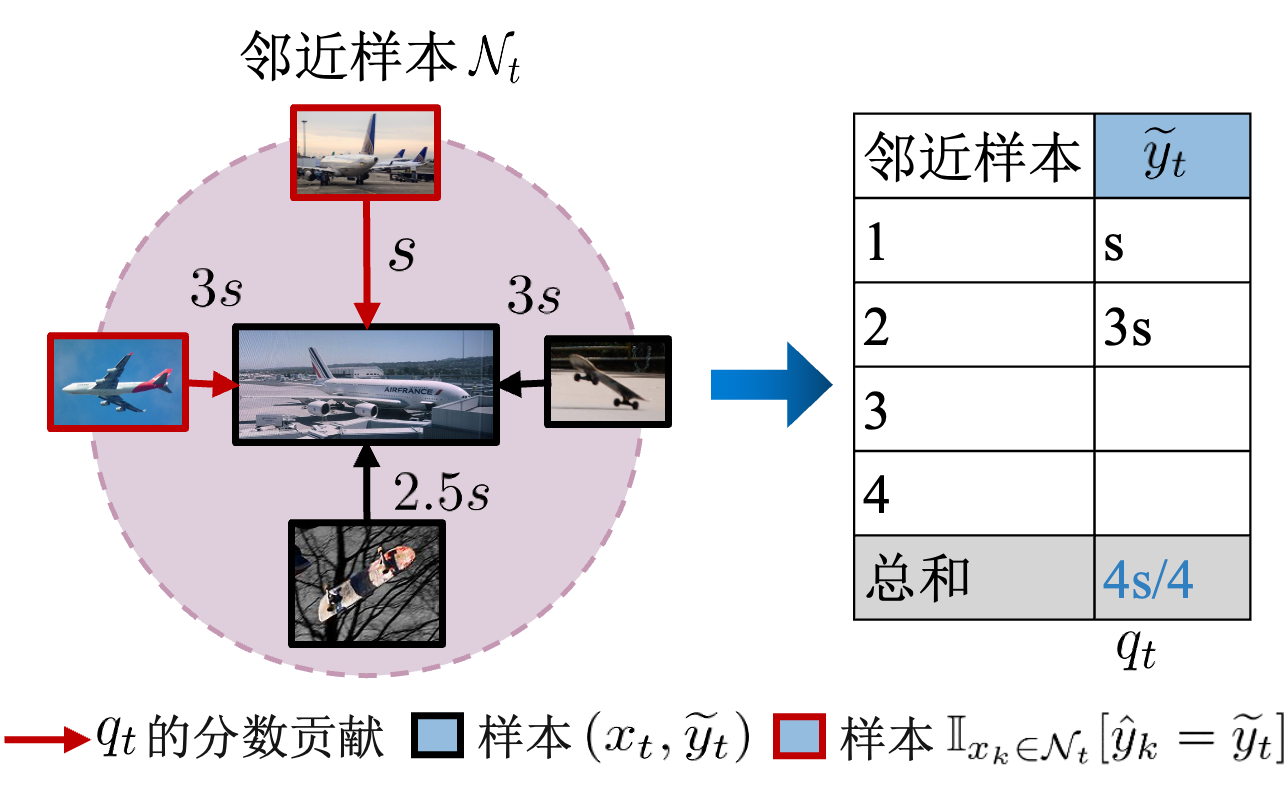
\includegraphics[width=0.55\textwidth]{figures/upa_extracted/v6_Aps.png}
  \bicaption[fig:confidence_score]{}{置信度评分 $q_t$ 的几何解释}{Fig.}{Geometric interpretation of confidence score $q_t$}
\end{figure}

此外，为避免在筛选过程中遗漏少数类，按 $q_t$ 对各类别内的样本分别排序，选取每个类别中得分最高的前 $\gamma_{\text{sel}}\%$ 的样本，组成干净伪标签样本集 $\mathcal{T}_c$。类别内排序策略在保证各类别均有样本入选的同时，使筛选阈值由类别内的置信度分布自适应决定。


\subsection{类感知对比学习策略}

\label{sec:chap2_upa_cacl}

尽管 APS 能够过滤大部分噪声伪标签，但仍不可避免地存在少量漏网的错误伪标签，以及类别边界区域的歧义样本。这些残余噪声会通过自训练回路在表征空间中被模型记忆，构成迁移不确定性的隐蔽来源。为此，本文提出类感知对比学习 CACL 策略，在干净伪标签样本集 $\mathcal{T}_c$ 上利用类别级对比学习增强类内语义一致性，阻断噪声记忆的传播。

对于每个样本 $x_i$，首先生成其强增强视图 $x_i'$，在大小为 $B_{\text{batch}}$ 的 mini-batch 中，我们定义$i\in \mathcal{I}=\{1,\cdots,2B_{\text{batch}}\}$, 若两个样本 $(x_i, y_i)$ 和 $(x_j, y_j)$ 均属于 $\mathcal{T}_c$ 且 $y_i = y_j$，则二者构成正样本对：
\begin{equation}
\mathcal{O}(i) = \left\{ o_{ij} \mid y_i = y_j;\ (x_i, y_i), (x_j, y_j) \in \mathcal{T}_c \right\},
\label{eq:positive_pairs}
\end{equation}
其中 $o_{ij} = \langle (x_i, y_i), (x_j, y_j) \rangle$，$j \in \mathcal{A}(i) \equiv \mathcal{I} \setminus \{i\}$。类别级对比损失形式化为：
\begin{equation}
\mathcal{L}_{\text{CL}} = \sum_{i \in \mathcal{I}} -\frac{1}{|\mathcal{J}(i)|} \sum_{j \in \mathcal{J}(i)} \log \frac{\exp(z_i \cdot z_j / \tau)}{\sum_{a \in \mathcal{A}(i)} \exp(z_i \cdot z_a / \tau)},
\label{eq:contrastive_loss}
\end{equation}
其中 $\mathcal{J}(i) = \{j \mid j \in \mathcal{A}(i), o_{ij} \in \mathcal{O}(i)\}$，$\tau$ 为温度参数，$z_i = g(x_i)/\|g(x_i)\|$ 为归一化特征。CACL 通过强增强视图间的类内一致性约束，增强目标域上的判别性表征，并有效阻断模型对残余噪声伪标签的记忆。


除 CACL 外，UPA 采用标准交叉熵损失引导模型在干净伪标签样本集上的学习：
\begin{equation}
\mathcal{L}_{\text{CE}} = -\mathbb{E}_{(x_t, \hat{y}_t) \in \mathcal{T}_c} \sum_{c=1}^{C} \mathbf{1}(c = \hat{y}_t) \log p_c(x_t),
\label{eq:ce_loss}
\end{equation}

最终总体损失为 $\mathcal{L} = \mathcal{L}_{\text{CL}} + \beta_{\text{CE}} \mathcal{L}_{\text{CE}} + \mathcal{L}_{\text{IM}}$。完整训练流程以渐进式适应方式交替执行 APS 伪标签筛选与基于总体损失的参数更新，如算法~\ref{alg:upa} 所示。

\begin{algorithm}[!htb]
  \AlgoBiCaption{UPA 算法训练流程}{Training procedure of UPA}
  \label{alg:upa} 
  \small
  \KwIn{无标签目标样本 $\mathcal{T}$，预训练源域模型 $\theta_s$；训练轮数 $\hat{T}$，每轮迭代数 $e_T$，批次大小 $B_{\text{batch}}$；超参数 $\gamma_{\text{sel}}, \tau, K, \beta_{\text{CE}}$}
  \KwOut{适应后的目标域模型 $\theta_t$}
  \BlankLine
  \For{epoch $= 1$ \textbf{to} $\hat{T}$}{
    基于式\eqref{eq:chap2_proto} 生成伪标签 $\hat{y}_t$\;
    % \tcp{// APS 模块}
    基于式\eqref{eq:knn_voting}--\eqref{eq:confidence} 计算置信度评分并选取 top $\gamma_{\text{sel}}\%$ 样本构成 $\mathcal{T}_c$\;
    \For{iter $= 1$ \textbf{to} $e_T$}{
      从 $\mathcal{T}$ 中采样小批量样本 $\{x_b\}_{b=1}^{B_{\text{batch}}}$\;
      基于式\eqref{eq:positive_pairs} 构建正样本对集合 $\mathcal{O}$\;
      $\theta_t \leftarrow \theta_t - \eta \nabla (\mathcal{L}_{\text{CL}} + \beta_{\text{CE}} \mathcal{L}_{\text{CE}} + \mathcal{L}_{\text{IM}})$;
    }
  }
  \Return $\theta_t$
\end{algorithm}


\section{基于选择性扫描的不确定性感知的迁移方法}

\label{sec:chap2_sfmamba}

UPA 从判别层去噪的角度抑制了伪标签噪声的累积，但其作用对象限于监督信号的可靠性，骨干自身的建模方式所引入的不确定性仍未被触及。为进一步控制跨域表征中的迁移不确定性，
本节在骨干网络层面引入状态空间模型 Mamba~\cite{gu2023mamba} 作为 SFDA 任务的骨干，并针对该骨干特有的表征层不确定性设计抑制机制。
Mamba定义了一类扫描序列到序列的映射，通过隐状态 $h(t) \in \mathbb{R}^N$ 将输入 $x(t)$ 映射为输出 $y(t)$，其状态转移参数是输入依赖的：$\Delta$、$B$、$C$ 均由当前输入 $x(t)$ 动态生成。连续时间常微分方程形式为：
\begin{equation}
h'(t) = A h(t) + B x(t), \quad y(t) = C h(t) + D x(t),
\label{eq:ssm_cont}
\end{equation}
其中 $A \in \mathbb{R}^{N \times N}$, $B \in \mathbb{R}^{N \times 1}$, $C \in \mathbb{R}^{1 \times N}$, $D \in \mathbb{R}$。离散化后形式化为：
\begin{equation}
h(t) = \overline{A} h(t-1) + \overline{B} x(t), \quad y(t) = C h(t) + D x(t).
\label{eq:ssm_disc}
\end{equation}

在视觉任务中，VMamba~\cite{liu2024vmamba} 将 Mamba 的序列建模扩展至二维图像，通过四向 2D 选择性扫描（沿行、列及对角线方向）捕获 patch 间的空间依赖关系。
这一性质使扫描过程承担了两项在视觉跨域场景中具有直接意义的功能。其一是长程依赖的线性聚合能力，状态 $h(t)$ 在时间维度上累积了此前全部位置的输入，因此相隔任意距离的两个 patch 之间仍存在直接的信息通路，这在 CNN 的固定局部感受野下并不存在；跨域偏移主要改变局部纹理统计而不改变图像的全局构成，长程依赖因此成为少数可跨域保持稳定的结构线索。其二是输入依赖的选择性，扫描状态可以依据当前输入的内容决定保留或跳过，从而抑制与判别无关的位置对状态演化的贡献。
% 据此，选择性扫描对跨域特征建模的作用可以解决“在何处聚合”与“聚合什么”两个可分离的问题。

% Mamba的关键改进是将时间尺度参数 $\Delta$ 与状态转移权重 $B$、$C$ 设计为输入序列 $x(t)$ 的动态函数，从而实现输入依赖的选择性扫描机制，使得 Mamba 能够在保持线性时间复杂度的同时，根据当前输入自适应调整状态转移行为。

与 CNN 骨干上迁移不确定性集中于判别层不同，Mamba 骨干下的迁移不确定性同时分布在表征层与序列层，构成其特有的双重不确定性问题：（1）表征层不确定性：VMamba 的选择性扫描主要沿空间维度展开，对跨通道频率域依赖建模不足~\cite{yang2020fda,qin2021fcanet}，如图~\ref{fig:cam_moti}，低频通道承载域不变的语义结构信息而高频通道更易受域差异干扰，源—目标域发生分布偏移时模型无法自适应强化语义稳定通道、抑制域敏感通道；（2）空间序列层不确定性：SSM 的隐藏状态演化依赖于输入序列的顺序，模型可能记忆源域扫描序列中前景与背景元素的空间共现模式（即“捷径学习”~\cite{geirhos2020shortcut}），如图~\ref{fig:scan}所示，当目标域打破这种空间配置时背景 patch 引入的虚假相关性会通过状态转移机制逐步累积放大，最终损害判别能力。这一序列层不确定性是 CNN 骨干上不存在、Mamba 序列建模独有的新风险。

\begin{figure}[!htbp]
  \centering
  \subfigure[ResNet101和VMamba-T的Grad-CAM可视化对比]{
    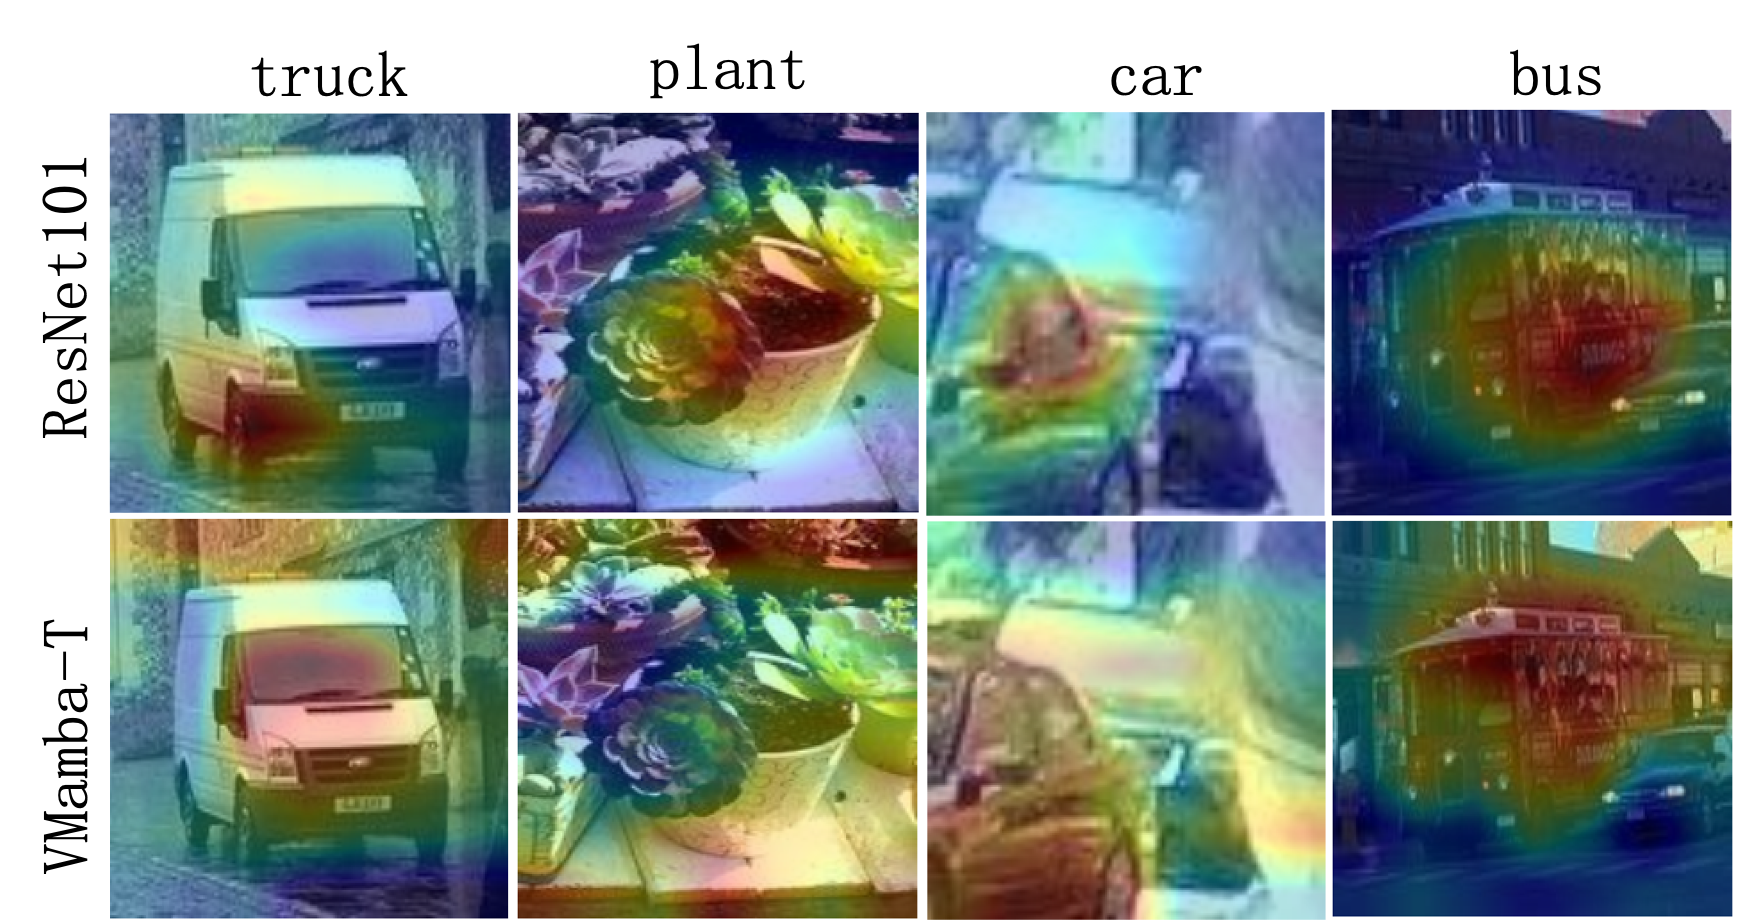
\includegraphics[width=0.48\textwidth]{figures/sfmamba/gradcam.png}
    \label{fig:cam_moti}
  }
  \hfill
  \subfigure[空间状态模型在域迁移下的错误预测传播阐述]{
    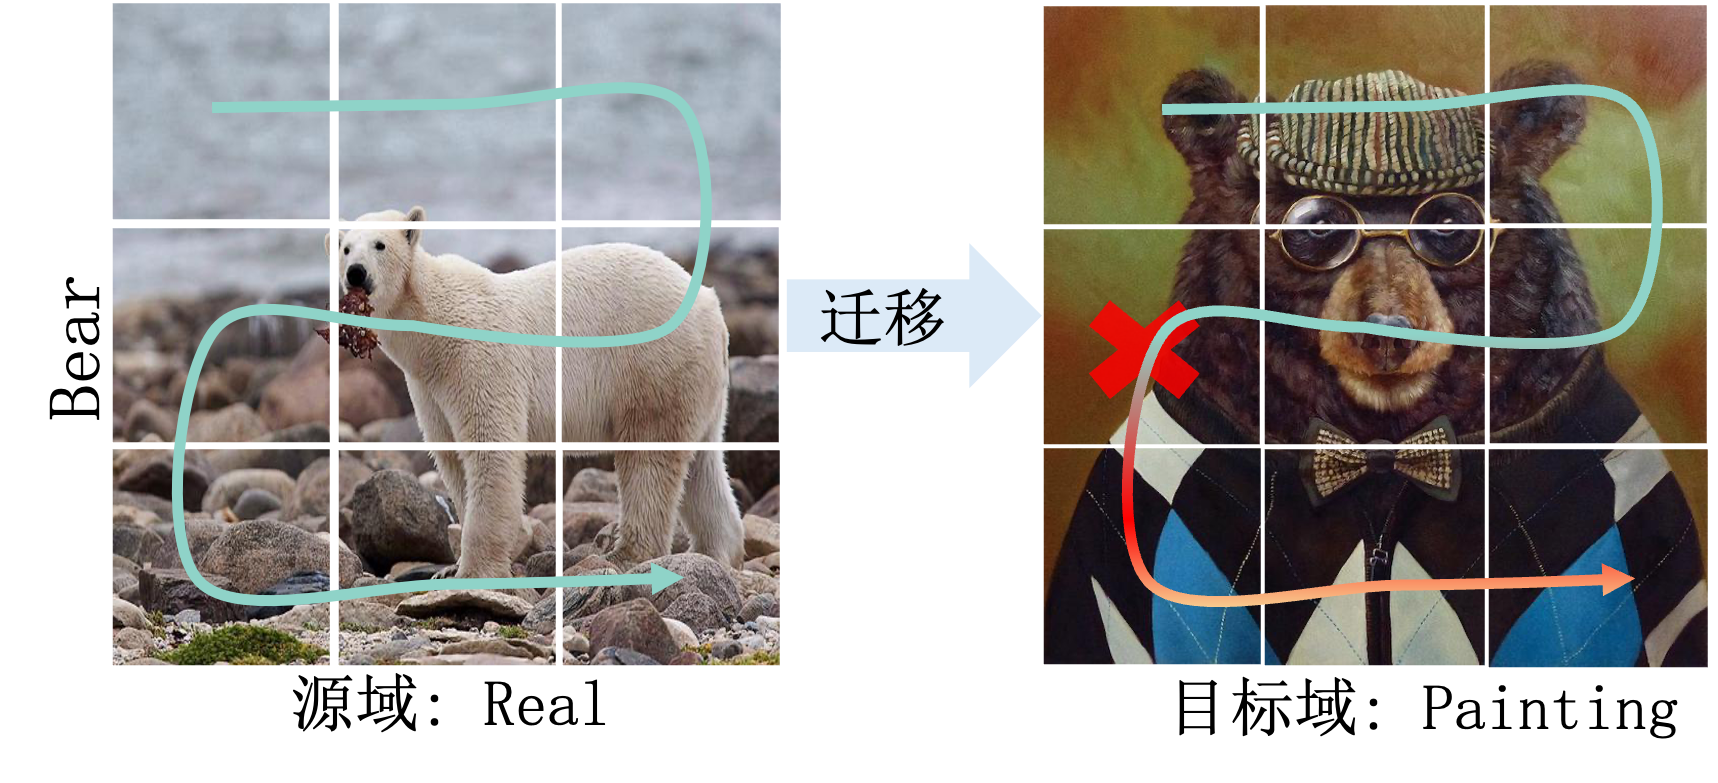
\includegraphics[width=0.48\textwidth]{figures/sfmamba/spatial_scanning.png}
    \label{fig:scan}
    }
    \bicaption[fig:sfmamba_uncertainty]{}{Mamba 骨干的迁移不确定性}{Fig.}{Transfer uncertainty of the Mamba backbone}
\end{figure}

本文提出SfMamba 针对上述两种不确定性分别设计抑制机制（图~\ref{fig:sfmamba_framework}）：通道级视觉状态空间模块 Ch-VSS 抑制表征层不确定性；语义一致性打乱策略抑制序列层不确定性。两条抑制路径共同实现对 SSM 骨干下迁移不确定性的协同治理。

\begin{figure}[!htbp]
    \centering
    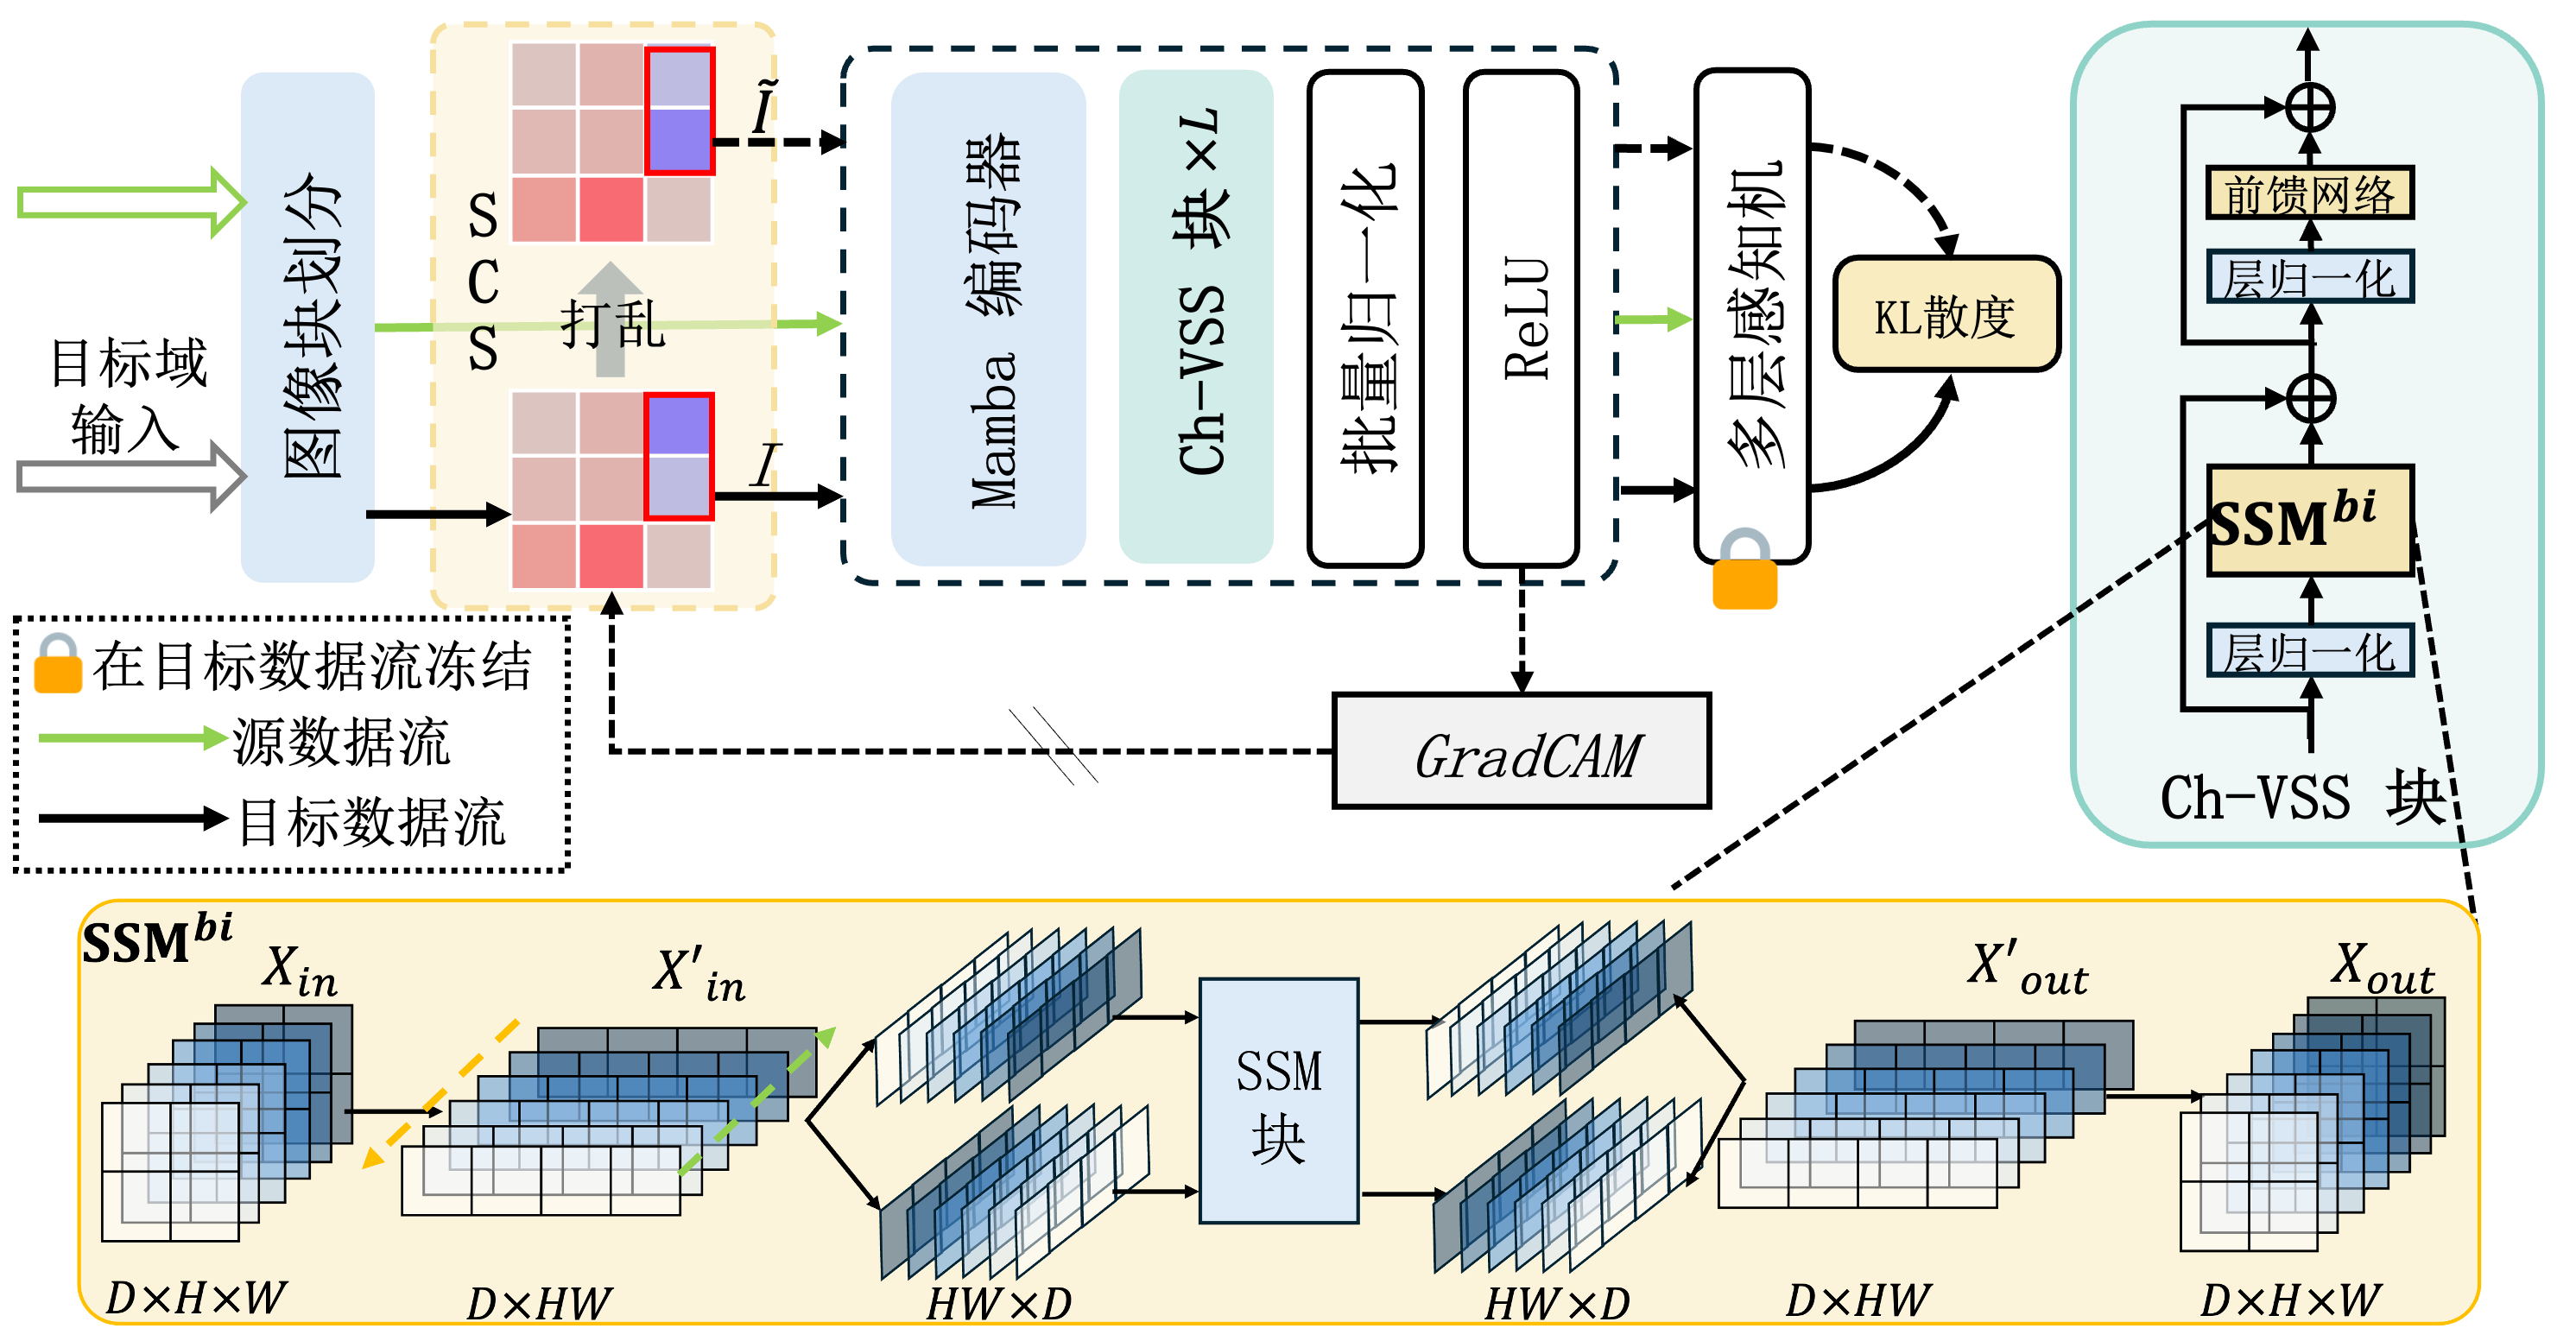
\includegraphics[width=0.95\textwidth]{figures/sfmamba/backbone.png}
    \bicaption[fig:sfmamba_framework]{}{SfMamba 总体框架}{Fig.}{Overview of SfMamba framework}
\end{figure}

\subsection{通道维度选择性扫描}

\label{sec:chap2_sfmamba_chvss}

视觉 VMamba 通过四向 2D 选择性扫描捕获 patch 间的空间长程依赖，但其在通道维度上的建模存在结构性短板：SSM 状态转移沿空间 token 顺序递归展开，每个时刻的状态更新仅与单一 patch 关联，跨通道频率域相关性需要等到所有空间 patch 完成扫描后通过后续通道投影间接获得，难以显式强化语义稳定的低频通道、抑制域敏感的高频通道。这一限制在源—目标域发生显著分布偏移时尤为突出：低频通道承载的跨域一致纹理与轮廓信息与高频通道承载的域特异细节在适应阶段出现响应失衡。
如图~\ref{fig:sfmamba_chvss_compare}，EMAN~\cite{EMAN}在多层重建框架内集成压缩后的通道注意力；DA-Mamba~\cite{DA-Mamba}通过域间通道混合实现跨域对齐。本章Ch-VSS 模块则采取非压缩的显式通道维度双向扫描策略，将通道相关性建模为可学习的跨域特征重组策略。

\begin{figure}[!htbp]
    \centering
    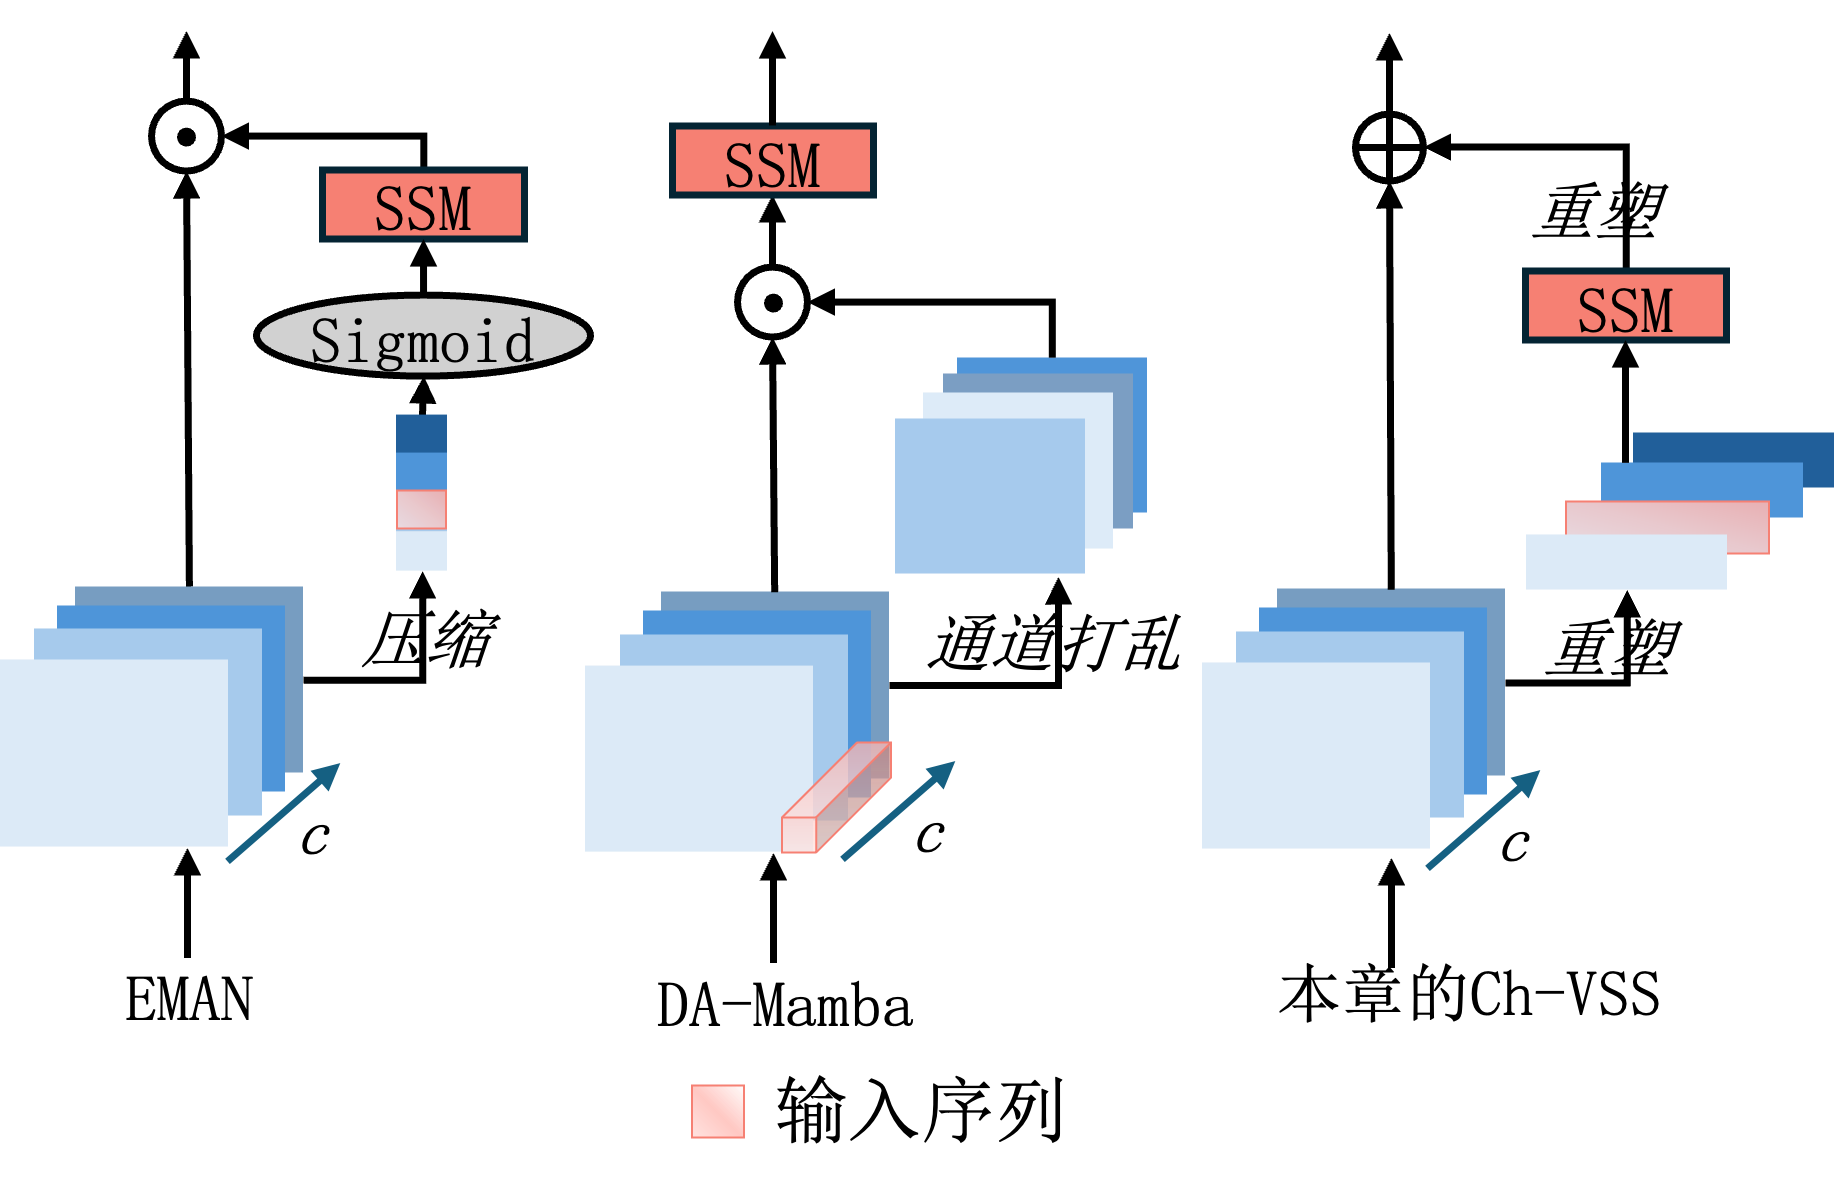
\includegraphics[width=0.6\linewidth]{figures/sfmamba/mamba_channel_atten.png}
    \bicaption[fig:sfmamba_chvss_compare]{}{本章Ch-VSS与其他Mamba工作的通道维度学习机制对比示意}{Fig.}{Comparison of channel-wise attention mechanisms integrated on the Mamba backbone}
\end{figure}

具体的，给定骨干网络特征图 $X_{\text{in}} = g(x^t) \in \mathbb{R}^{D \times H \times W}$，Ch-VSS 首先将其重塑为通道向量序列 $X'_{\text{in}} \in \mathbb{R}^{D \times (HW)}$，然后沿通道维度应用双向 SSM，以缓解单向扫描带来的通道顺序偏置：
\begin{align}
    X'_{\rightarrow} &= \text{SSM}(X'_{\text{in}}), \quad
    X'_{\leftarrow} = \text{SSM}\!\big(\textit{Reverse}(X'_{\text{in}})\!\big), \notag \\
    X'_{\text{out}} &= \text{SSM}_{\text{bi}}(X'_{\text{in}}) = X'_{\leftarrow} + \textit{Reverse}(X'_{\rightarrow}) \in \mathbb{R}^{D \times (HW)},
    \label{eq:ch_scan}
\end{align}
其中正向扫描沿 $1 \rightarrow D$ 方向聚合通道信息，反向扫描沿 $D \rightarrow 1$ 方向聚合，最终通过融合两侧响应获得与通道顺序无关的全局依赖。处理后的序列被重塑回特征图 $X_{\text{out}} \in \mathbb{R}^{D \times H \times W}$，并通过残差连接与原始特征相加以保留骨干网络的空间结构信息。Ch-VSS 整体作为辅助 neck 网络嵌入模型末端，可形式化为：
\begin{equation}
    \theta_t(x^t) = f\!\left(\text{Ch-VSS}\!\big(g(x^t)\big)\right).
    \label{eq:sf_chvss_out}
\end{equation}

通道维度扫描对表征层不确定性的抑制体现在两个方面：（1）双向通道扫描直接建模跨通道的频率域相关性，使模型自适应强化语义稳定的低频通道、抑制域敏感的高频通道；（2）通道扫描捕获跨域一致的基础模式（如边缘检测器、纹理基元），这些模式在源—目标域分布偏移下保持稳定，从而构成“域不变基础特征”。


% Ch-VSS 本质上学习的是一种“通道维度的特征重组策略”，即通过双向通道扫描建立不同频率域通道之间的关联模式。这种关联模式需要在源域数据上进行充分的监督学习才能稳定建立。实验表明：仅在目标域适应阶段引入随机初始化或零初始化~\cite{zhang2023adding} 的 Ch-VSS 相比基线无显著改善，验证了源域预训练是 Ch-VSS 发挥表征层不确定性抑制作用的必要前提。

\subsection{空间2D选择性扫描}

\label{sec:chap2_sfmamba_scs}

为抑制空间2D维度 SSM 序列建模中的虚假相关累积，本文提出了语义一致性打乱 SCS 策略。SCS 的核心思想是：通过打乱背景 patch 的顺序打破虚假的空间相关性，同时通过一致性正则迫使模型在不依赖空间配置的情况下维持预测。

SCS 在 patch 粒度上操作。沿用 VMamba 的 patch 嵌入向量设定，特征图被划分为大小 $p \times p$、步长 $p$ 的非重叠 patch，对于空间分辨率 $H \times W$ 的特征图，共产生 $N_p = (H/p) \times (W/p)$ 个 patch token。GradCAM~\cite{selvaraju2017grad} 在骨干网络末端层生成的激活图谱被重采样至 patch 分辨率，并在每个 patch 区域内聚合为一个 patch 级别的重要性得分。基于此得分，识别相对于伪标签 $\hat{y}$ 激活值最低的 $\gamma_{\text{bg}}\%$ 的 patch 作为背景 patch 集合 $\{P_k\}_{k=1}^{N_p}$。这些背景 patch 在源域中往往与目标对象存在稳定的共现关系，是空间捷径学习的主要载体。
所以本文通过随机置换矩阵 $\Pi$ 对背景 patch 进行重排：
\begin{equation}
\tilde{P}_k = P_{\Pi(k)}, \quad \tilde{U} = \text{Replace}(U, \{\tilde{P}_k\}),
\label{eq:shuffle}
\end{equation}
得到扰动序列 $\tilde{U}$。该操作在 VMamba 的四条 2D 扫描路径（沿行、列、两条对角线方向）上均会破坏固定的上下文关系（如图~\ref{fig:sfmamba_scs_compare}），使模型无法再依赖“前景—背景”空间共现进行预测，从根源上切断序列层迁移不确定性的累积链路。


\begin{figure}[!htbp]
    \centering
    \includegraphics[width=0.7\linewidth]{papers/Sfmamba/scs.pdf}
    \bicaption[fig:sfmamba_scs_compare]{}{SCS 策略描述图}{Fig.}{The illustration of the SCS strategy}
\end{figure}

为保证打乱操作不损害模型对前景语义的判别能力，引入 KL 散度一致性正则：
\begin{equation}
\mathcal{L}_{\text{KL}} = \mathbb{E}_{x^t \sim \mathcal{T}} D_{\text{KL}}\!\left(\theta_t(U) \,\|\, \theta_t(\tilde{U})\right),
\label{eq:kl_loss}
\end{equation}
迫使模型在原始序列与打乱序列上的输出分布保持一致。这一约束使 SSM 的隐藏状态演化主要依赖鲁棒的前景特征，而非背景序列的顺序，从而抑制 SSM 序列建模独有的序列层迁移不确定性。

% \subsection{邻居感知去噪与总体训练流程}
% \label{sec:chap2_sfmamba_training}


% 整体训练沿用 §2.3 APS 框架的迭代式伪标签精炼—损失更新循环，体现两条方法路线在抑制判别层不确定性上的模块级可组合性。两路径对迁移不确定性的整体抑制结构可总结为：UPA 以邻居一致性提供判别层去噪，SfMamba 在其基础上以 Ch-VSS 抑制表征层不确定性、以 SCS 抑制序列层不确定性，三层叠加形成对迁移不确定性的协同抑制。


\noindent\textbf{总体训练流程}

\label{sec:chap2_sfmamba_training}

上述判别层去噪与骨干级序列增强在同一次参数更新中协同作用。为缓解伪标签噪声对 $\mathcal{L}_{\text{CE}}$ 与 $\mathcal{L}_{\text{KL}}$ 的负面影响，SfMamba 采用§\ref{sec:chap2_upa_denoising}的邻居一致性筛选策略作为子组件：对每个目标样本 $x^t$ 构建 K 近邻集合 $\mathcal{N}_t$ 并迭代估计精炼伪标签 $\hat{y}'$ 与置信度评分 $q_t$，按类别内排序选取前 $\gamma_{\text{sel}}\%$ 样本构成高置信子集 $\mathcal{T}_c$，仅在该子集上计算 $\mathcal{L}_{\text{CE}}$ 与 $\mathcal{L}_{\text{KL}}$：
\begin{equation}
\mathcal{L}_{\text{CE}} = -\mathbb{E}_{x^t \in \mathcal{T}_c} \sum_{c=1}^{C} \hat{y}_c \log p_c(x^t), \quad
\mathcal{L}_{\text{KL}} = \mathbb{E}_{x^t \in \mathcal{T}_c} D_{\text{KL}}\!\left(\theta_t(U) \,\|\, \theta_t(\tilde{U})\right).
\label{eq:scs_loss_ch}
\end{equation}

最终，SfMamba 的总体训练损失为：
\begin{equation}
\mathcal{L} = \mathcal{L}_{\text{KL}} + \mathcal{L}_{\text{ent}} + \mathcal{L}_{\text{div}} + \mathcal{L}_{\text{CE}},
\label{eq:scs_total_loss}
\end{equation}
其中 $\mathcal{L}_{\text{ent}}$ 与 $\mathcal{L}_{\text{div}}$ 的形式化参见式~\eqref{eq:chap2_im}。

完整训练流程以渐进式适应方式交替执行 APS 伪标签筛选与基于总体损失的参数更新，如算法~\ref{alg:sfmamba} 所示。

\begin{algorithm}[!htb]
  \AlgoBiCaption{SfMamba 算法训练流程}{Training procedure of SfMamba}
  \label{alg:sfmamba}
  \small
  \KwIn{无标签目标样本 $\mathcal{T}$，预训练源域模型 $\theta_s$；训练轮数 $\hat{T}$，每轮迭代数 $e_T$，批次大小 $B_{\text{batch}}$；超参数 $\gamma_{\text{sel}}, \gamma_{\text{bg}}, K$}
  \KwOut{适应后的目标域模型 $\theta_t$}
  \BlankLine
  \For{epoch $= 1$ \textbf{to} $\hat{T}$}{
    基于式\eqref{eq:chap2_proto} 生成伪标签 $\hat{y}_t$\;
    基于式\eqref{eq:knn_voting}--\eqref{eq:confidence} 计算置信度评分并选取 top $\gamma_{\text{sel}}\%$ 样本构成 $\mathcal{T}_c$\;
    \For{iter $= 1$ \textbf{to} $e_T$}{
      从 $\mathcal{T}_c$ 中采样小批量样本 $\{x_b\}_{b=1}^{B_{\text{batch}}}$\;
      基于式\eqref{eq:shuffle} 置换背景 patch 得到扰动序列 $\tilde{U}$\;
      $\theta_t \leftarrow \theta_t - \eta \nabla (\mathcal{L}_{\text{KL}} + \mathcal{L}_{\text{ent}} + \mathcal{L}_{\text{div}} + \mathcal{L}_{\text{CE}})$;
    }
  }
  \Return $\theta_t$
\end{algorithm}

上述训练流程表明，判别层去噪与骨干级序列增强在同一次参数更新中协同作用：APS 以邻居一致性提供判别层去噪，Ch-VSS 抑制表征层不确定性，SCS 抑制序列层不确定性，三层叠加共同形成对迁移不确定性的系统性抑制。

\section{实验结果与分析}

\label{sec:chap2_experiments}

本章两条方法在统一的实验协议下评估，覆盖 Office、Office-Home、VisDA-C 与 DomainNet-126 四个跨域基准。主表按骨干网络分类组织，使同一骨干下的方法可在公平条件下比较；消融实验则按抑制机制归类，在卷积骨干与状态空间骨干上分别考察各机制的独立贡献及其互补性。以下先给出数据集与实现细节，再报告主实验结果，最后给出消融实验、可视化分析与计算效率分析。

\subsection{数据集与实验设置}

本节在 Office~\cite{saenko2010adapting}、Office-Home~\cite{venkateswara2017deep}、VisDA-C~\cite{peng2017visda} 与 DomainNet-126~\cite{peng2019moment} 四个基准数据集上评估所提的两条方法。具体而言：Office 数据集包含 Amazon（A）、Dslr（D）与 Webcam（W）三个域，域间共享 31 个类别；Office-Home 数据集包含 Art（A）、Clipart（C）、Product（P）与 Real World（R）四个域，每个域共享 65 个类别；VisDA-C 数据集包含合成域 Synthetic（S）与真实域 Real（R）的跨域分割任务；DomainNet-126 包含 126 个类别，来自 Real（R）、Painting（P）、Clipart（C）与 Sketch（S）四个域。

UPA 在卷积骨干上评估：Office、Office-Home 与 DomainNet-126 使用 ResNet-50，VisDA-C 使用 ResNet-101，源域模型采用 SHOT 的预训练设置。适应阶段采用 SGD 优化器，设置动量 0.9、权重衰减 $10^{-3}$、batch size 64，学习率策略为先线性预热一个 epoch 后余弦退火衰减；Office、Office-Home 与 DomainNet-126 的初始学习率设为 $10^{-2}$，VisDA-C 的初始学习率设为 $10^{-3}$，瓶颈层学习率设置为骨干网络的 10 倍。损失权重 $\beta_{\text{CE}} = 0.3$，对比温度 $\tau = 0.1$，近邻数 $K = 4$，置信样本筛选比例 $\gamma_{\text{sel}}$ 在 Office / Office-Home / DomainNet-126 设为 0.6，在 VisDA-C 设为 0.8。

SfMamba 在状态空间骨干上评估：采用 VMamba-T（Tiny）与 VMamba-S（Small）两种规模的 SSM 骨干，并以 SHOT~\cite{liang2021source} 自训练框架为基础，冻结分类器。训练阶段采用 AdamW 优化器，权重衰减率为 $5 \times 10^{-2}$，并用余弦退火策略，批次大小为 32，在单卡 NVIDIA RTX A100 GPU 进行实验。源域预训练 Office / Office-Home / VisDA-C / DomainNet-126 分别为 100 / 50 / 10 / 30 个 epoch，目标域适应阶段背景比例 $\gamma_{\text{bg}} = 20\%$，近邻数 $K = 4$，置信样本筛选比例 $\gamma_{\text{sel}}$ 在 Office-Home 与 DomainNet-126 设为 0.6，在 VisDA-C 设为 0.8。所有结果报告三次随机种子 $\{0, 1, 2\}$ 的平均值。


\subsection{实验结果对比}

以下分别在 Office-Home、VisDA-C、Office 与 DomainNet-126 四个基准上报告实验结果。其中 Office-Home 与 VisDA-C 的对比方法按骨干网络分类合并于同一张表内，Office 与 DomainNet-126 各自成表。

\noindent\textbf{Office-Home 与 VisDA-C}

\begin{table}[!htbp]
  \bicaption[tab:main_oh_visda]{}{Office-Home 与 VisDA-C 数据集上的准确率对比}{Table}{Accuracy comparison on Office-Home and VisDA-C, grouped by backbone architecture}
  \vspace{0.5em}\centering\wuhao
  \setlength{\tabcolsep}{1pt}
  \resizebox{\textwidth}{!}{
  \begin{tabular}{lc*{13}{c}c}
  \toprule
  \multirow{2}*{方法} & \multirow{2}*{SF} & \multicolumn{13}{c}{Office-Home} & \multicolumn{1}{c}{VisDA-C} \\
  \cline{3-16}
  & & A$\rightarrow$C & A$\rightarrow$P & A$\rightarrow$R & C$\rightarrow$A & C$\rightarrow$P & C$\rightarrow$R & P$\rightarrow$A & P$\rightarrow$C & P$\rightarrow$R & R$\rightarrow$A & R$\rightarrow$C & R$\rightarrow$P & Avg & S$\rightarrow$R \\
  \midrule
  \multicolumn{16}{c}{\textit{基于CNN的方法}} \\
  \midrule
  ResNet~\cite{he2016deep} & \checkmark & 44.0 & 65.9 & 74.0 & 52.1 & 61.0 & 65.4 & 52.2 & 40.9 & 72.9 & 64.1 & 45.3 & 77.9 & 59.6 & 47.8 \\
  SHOT~\cite{liang2021source} & \checkmark & 57.1 & 78.1 & 81.5 & 68.0 & 78.2 & 78.1 & 67.4 & 54.9 & 82.2 & 73.3 & 58.8 & 84.3 & 71.8 & 82.9 \\
  % MCC~\cite{MCC} & $\times$ & -- & -- & -- & -- & -- & -- & -- & -- & -- & -- & -- & -- & -- & 78.8 \\
  % BCDM~\cite{BCDM} & $\times$ & -- & -- & -- & -- & -- & -- & -- & -- & -- & -- & -- & -- & -- & 83.4 \\
  % CAN~\cite{CAN} & $\times$ & -- & -- & -- & -- & -- & -- & -- & -- & -- & -- & -- & -- & -- & 87.2 \\
  % 3C-GAN~\cite{3C-GAN} & \checkmark & -- & -- & -- & -- & -- & -- & -- & -- & -- & -- & -- & -- & -- & 81.6 \\
  % HCL~\cite{HCL} & \checkmark & -- & -- & -- & -- & -- & -- & -- & -- & -- & -- & -- & -- & -- & 83.5 \\
  % SSNLL~\cite{chen2022self} & \checkmark & -- & -- & -- & -- & -- & -- & -- & -- & -- & -- & -- & -- & -- & 86.0 \\
  % CDCL~\cite{wang2022cross} & \checkmark & -- & -- & -- & -- & -- & -- & -- & -- & -- & -- & -- & -- & -- & 87.5 \\
  % AdaContrast~\cite{AdaContrast} & \checkmark & -- & -- & -- & -- & -- & -- & -- & -- & -- & -- & -- & -- & -- & 86.8 \\
  CDAN~\cite{CDAN} & $\times$ & 50.7 & 70.6 & 76.0 & 57.6 & 70.0 & 70.0 & 57.4 & 50.9 & 77.3 & 70.9 & 56.7 & 81.6 & 65.8 & 73.9 \\
  MDD~\cite{MDD} & $\times$ & 54.9 & 73.7 & 77.8 & 60.0 & 71.4 & 71.8 & 61.2 & 53.6 & 78.1 & 72.5 & 60.2 & 82.3 & 68.1 & -- \\
  VDM-DA~\cite{tian2022vdm} & \checkmark & 59.3 & 75.3 & 78.3 & 67.6 & 76.0 & 75.9 & 68.8 & 57.7 & 79.6 & 74.0 & 61.1 & 83.6 & 71.4 & 85.3 \\
  D-MCD~\cite{chu2022denoised} & \checkmark & 59.4 & 78.9 & 80.2 & 67.2 & 79.3 & 78.6 & 65.3 & 55.6 & 82.2 & 73.3 & 62.8 & 83.9 & 72.2 & 87.5 \\
  DIPE~\cite{DIPE} & \checkmark & 56.5 & 79.2 & 80.7 & 70.1 & 79.8 & 78.8 & 67.9 & 55.1 & 83.5 & 74.1 & 59.3 & 84.8 & 72.5 & 83.1 \\
  
  FixBi~\cite{FIxBi} & $\times$ & 58.1 & 77.3 & 80.4 & 67.7 & 79.5 & 78.1 & 65.8 & 57.9 & 81.7 & 76.4 & 62.9 & 86.7 & 72.7 & 87.2 \\
  U-SFAN~\cite{U-SFAN} & \checkmark & 57.8 & 77.8 & 81.6 & 67.9 & 77.3 & 79.2 & 67.2 & 54.7 & 81.2 & 73.3 & 60.3 & 83.9 & 71.9 & 82.7 \\
  NRC~\cite{yang2021neighbor} & \checkmark & 57.7 & 80.3 & 82.0 & 68.1 & 79.8 & 78.6 & 65.3 & 56.4 & 83.0 & 71.0 & 58.6 & 85.6 & 72.2 & 85.9 \\
  CoWA-JMDS~\cite{cowa} & \checkmark & 56.9 & 78.4 & 81.0 & 69.1 & 80.0 & 79.9 & 67.7 & 57.2 & 82.4 & 72.8 & 60.5 & 84.5 & 72.5 & 86.9 \\
  NAMI~\cite{zhang2024neighborhood} & \checkmark & 58.3 & 80.9 & 82.9 & 68.5 & 80.5 & 79.6 & 66.0 & 57.0 & 83.7 & 71.9 & 59.9 & 85.0 & 72.9 & \underline{88.9} \\
  本章UPA~\cite{UPA} & \checkmark & 57.3 & 79.5 & 82.4 & 68.2 & 81.0 & 80.2 & 69.3 & 55.4 & 82.3 & 75.3 & 59.2 & 85.5 & 73.0 & 88.7 \\
  % TPWA~\cite{tpwa} & \checkmark & 58.8 & 80.3 & 82.4 & 69.5 & 80.6 & 78.8 & 68.4 & 55.8 & 82.0 & 74.7 & 59.2 & 85.5 & 73.0 & 87.2 \\
  % SHOT+DPC~\cite{dpc} & \checkmark & 59.2 & 79.8 & 82.6 & 68.9 & 79.7 & 79.5 & 68.6 & 56.5 & 82.9 & 73.9 & 61.2 & 85.4 & 73.2 & 84.3 \\
  % I-SFDA~\cite{mitsuzumi2024understanding} & \checkmark & 60.7 & 78.9 & 82.0 & 69.9 & 79.5 & 79.7 & 67.1 & 58.8 & 82.3 & 74.2 & 61.3 & 86.4 & 73.4 & 88.4 \\
  % C-SFDA~\cite{karim2023c} & \checkmark & 60.3 & 80.2 & 82.9 & 69.3 & 80.1 & 78.8 & 67.3 & 58.1 & 83.4 & 73.6 & 61.3 & 86.3 & 73.5 & 87.8 \\
  % TPDS~\cite{tang2023tpds} & \checkmark & 59.3 & 80.3 & 82.1 & 70.6 & 79.4 & 80.9 & 69.8 & 56.8 & 82.1 & 74.5 & 61.2 & 85.3 & 73.5 & 87.6 \\
  % DPL~\cite{xia2024dual} & \checkmark & 60.9 & 80.8 & 82.3 & 69.9 & 79.5 & 80.0 & 70.0 & 57.0 & 82.7 & 75.7 & 63.0 & 86.0 & 74.0 & 87.8 \\
  % RGV~\cite{zhu2025revisiting} & \checkmark & 61.2 & 80.9 & 82.7 & 69.3 & 81.2 & 81.4 & 68.1 & 58.8 & 83.4 & 74.6 & 62.4 & 85.7 & 74.1 & \underline{89.1} \\
  % DAPL~\cite{ge2023domain} & $\times$ & 54.1 & 84.3 & 84.8 & 74.4 & 83.7 & 85.0 & 74.5 & 54.6 & 84.8 & 75.2 & 54.7 & 83.8 & 74.5 & 86.9 \\
  \midrule
  \multicolumn{16}{c}{\textit{基于ViT的方法}} \\
  \midrule
  DeiT-S~\cite{deit} & \checkmark & 55.6 & 73.0 & 79.4 & 70.6 & 72.9 & 76.3 & 67.5 & 51.0 & 81.0 & 74.5 & 53.2 & 82.7 & 69.8 & - \\
  DeiT-B~\cite{deit} & \checkmark & 61.8 & 79.5 & 84.3 & 75.4 & 78.8 & 81.2 & 72.8 & 55.7 & 84.4 & 78.3 & 59.3 & 86.0 & 74.8 & 67.1 \\
  CDTrans-S~\cite{xu2022cdtrans} & $\times$ & 60.6 & 79.5 & 82.4 & 75.6 & 81.0 & 82.3 & 72.5 & 56.7 & 84.4 & 77.0 & 59.1 & 85.5 & 74.7 & - \\
  SHOT-B~\cite{liang2021source} & \checkmark & 67.1 & 83.5 & 85.5 & 76.6 & 83.4 & 83.7 & 76.3 & 65.3 & 85.3 & 80.4 & 66.7 & 83.4 & 78.1 & 83.5 \\
  CDTrans-B~\cite{xu2022cdtrans} & $\times$ & 68.8 & \underline{85.0} & 86.9 & \underline{81.5} & \underline{87.1} & \underline{87.3} & \underline{79.6} & 63.3 & \underline{88.2} & 82.0 & 66.0 & \underline{90.6} & 80.5 & 88.4 \\
  DSiT-B~\cite{sanyal2023domain} & \checkmark & 69.2 & 83.5 & 87.3 & 80.7 & 86.1 & 86.2 & 77.9 & \underline{67.9} & 86.6 & 82.4 & 68.3 & 89.8 & 80.5 & 87.6 \\
  C-SFTrans~\cite{sanyal2024aligning} & \checkmark & \underline{70.3} & 83.9 & 87.3 & 80.2 & 86.9 & 86.1 & 78.9 & 65.0 & 87.7 & \underline{82.6} & 67.9 & 90.2 & 80.6 & 88.3 \\
  \midrule
  \multicolumn{16}{c}{\textit{基于Mamba的方法}} \\
  \midrule
  Source-T & \checkmark & 59.0 & 76.8 & 83.0 & 69.8 & 76.5 & 78.2 & 68.9 & 54.6 & 82.4 & 74.8 & 58.3 & 85.4 & 72.3 & 61.5 \\
  Source-S & \checkmark & 62.9 & 79.5 & 84.7 & 74.4 & 80.2 & 81.2 & 71.9 & 56.9 & 84.4 & 78.4 & 61.9 & 86.6 & 75.3 & 65.6 \\
  SHOT-T$^\dagger$~\cite{liang2021source} & \checkmark & 64.9 & 80.1 & 83.6 & 75.4 & 81.4 & 81.3 & 71.7 & 60.7 & 84.9 & 77.4 & 66.1 & 87.7 & 76.3 & 81.9 \\
  SHOT-S$^\dagger$~\cite{liang2021source} & \checkmark & 67.3 & 81.5 & 85.6 & 79.9 & 85.3 & 83.8 & 76.1 & 66.4 & 85.3 & 80.1 & 69.0 & 88.7 & 79.1 & 84.6 \\
  本章SfMamba-T & \checkmark & 67.5 & 80.9 & 87.4 & 77.6 & 83.4 & 86.4 & 76.2 & 66.1 & 86.9 & 78.7 & \underline{69.6} & 89.8 & 79.2 & 88.5 \\
  DATMamba~\cite{gao2025datmamba} & \checkmark & 67.1 & \textbf{86.3} & \underline{87.8} & \textbf{81.7} & \textbf{87.3} & 85.4 & \textbf{80.2} & 66.3 & 87.1 & \textbf{83.2} & 67.6 & 90.5 & \underline{80.9} & \underline{88.9} \\
  本章SfMamba-S & \checkmark & \textbf{71.2} & 84.5 & \textbf{88.4} & \textbf{81.7} & 85.9 & \textbf{88.0} & 79.0 & \textbf{69.3} & \textbf{88.5} & 81.1 & \textbf{72.1} & \textbf{90.7} & \textbf{81.7} & \textbf{89.3} \\
  \bottomrule
  \end{tabular}
  }
\end{table}

表~\ref{tab:main_oh_visda} 展示了在 Office-Home 数据集上的结果。源域仅训练阶段 Source-T 即取得 72.3\% 的基线精度，高于 ResNet-50 的 59.6\% 与 DeiT-S 的 69.8\% 等源域基线，验证了 SSM 骨干在源域预训练阶段的长程建模优势。完整 SfMamba-S 取得 81.7\% 平均精度，刷新该基准 SFDA 方法最优纪录，在 12 个跨域任务中斩获 8 项最佳，分别超过此前最优 ViT 基方法 C-SFTrans 与最优 Mamba 基方法 DATMamba；轻量版本 SfMamba-T 以 79.2\% 取得与强 ViT 基方法相当的性能。这些结果表明 SfMamba 有效增强了跨域特征的可迁移性。

在 VisDA-C 大规模合成（S）→真实（R）跨域设定下，表~\ref{tab:main_oh_visda}中展示，SfMamba-S 达到 89.3\%，较此前最优 ViT 基 SFDA 方法 C-SFTrans 高 1.0 个百分点，并高于依赖源域数据的 CDTrans-B；轻量版本 SfMamba-T 以 39.0M 参数取得 88.5\%，与 DATMamba性能相当，且高于 CNN 基线 SHOT与 ViT 基线 SHOT-B。尤为关键的是，源域仅含 Ch-VSS 通道增强的 Source-S 基线在 VisDA-C 上仅取得 65.6\%，而完整 SfMamba 在此基础上提升 23.7 个百分点 至 89.3\%，验证了 SCS 对极端域迁移下序列层捷径学习的有效抑制。

如~\ref{tab:main_oh_visda}的 VisDA-C 列所示，判别层去噪方法 UPA~\cite{UPA} 在 VisDA-C 数据集上取得 88.7\% 的平均分类精度，显著超越 SHOT 基线方法，提升幅度达 5.8 个百分点，说明邻居一致性驱动的 APS 在过滤伪标签噪声方面具有明显效果。与此前最先进的 SFDA 方法 D-MCD 相比，UPA 仍高出 1.2 个百分点；而完整 SfMamba 在此基础上进一步提升至 89.3\%，验证了判别层去噪与骨干级序列增强叠加后的额外收益。

\noindent\textbf{Office}

\begin{table}[!htbp]
  \bicaption[tab:main_office]{}{Office 数据集上的准确率对比}{Table}{Accuracy comparison on Office, grouped by backbone architecture}
  \vspace{0.5em}\centering\wuhao
  % \renewcommand{\arraystretch}{1.3} 
  % \resizebox{.7\textwidth}{!}{
  \begin{tabular}{lc*{7}{c}}
  \toprule
  方法 & SF & A$\rightarrow$D & A$\rightarrow$W & D$\rightarrow$A & D$\rightarrow$W & W$\rightarrow$A & W$\rightarrow$D & Avg \\
  \midrule
  \multicolumn{9}{c}{\textit{基于CNN的方法}} \\
  \midrule
  ResNet~\cite{he2016deep} & \checkmark & 79.3 & 72.6 & 60.0 & 93.7 & 61.6 & 96.0 & 77.2 \\
  SHOT~\cite{liang2021source} & \checkmark & 94.0 & 90.1 & 74.7 & 98.4 & 74.3 & \underline{99.9} & 88.6 \\
  CDAN~\cite{CDAN} & $\times$ & 92.9 & 94.1 & 71.0 & 98.6 & 69.3 & \textbf{100.0} & 87.7 \\
  MDD~\cite{MDD} & $\times$ & 93.5 & 94.5 & 74.6 & 98.4 & 72.2 & \textbf{100.0} & 88.9 \\
  VDM-DA~\cite{tian2022vdm} & \checkmark & 94.1 & 93.2 & 75.8 & 98.0 & 77.1 & \textbf{100.0} & 89.7 \\
  3C-GAN~\cite{3C-GAN} & \checkmark & 92.7 & 93.7 & 75.3 & 98.5 & 77.8 & 99.8 & 89.6 \\
  D-MCD~\cite{chu2022denoised} & \checkmark & 94.1 & 93.5 & 76.4 & 98.8 & 76.4 & \textbf{100.0} & 89.9 \\
  NRC~\cite{yang2021neighbor} & \checkmark & 96.0 & 90.8 & 75.3 & 99.0 & 75.0 & \textbf{100.0} & 89.4 \\
  % SHOT+DPC~\cite{dpc} & \checkmark & 95.9 & 92.6 & 75.4 & 98.6 & 76.2 & \textbf{100.0} & 89.8 \\
  % TPWA~\cite{tpwa} & \checkmark & 96.2 & 95.2 & 75.8 & 98.8 & 75.6 & 99.2 & 90.1 \\
  DIPE~\cite{DIPE} & \checkmark & 96.6 & 93.1 & 75.5 & 98.4 & 77.2 & 99.6 & 90.1 \\
  % TPDS~\cite{tang2023tpds} & \checkmark & \underline{97.1} & 94.5 & 75.7 & 98.7 & 75.5 & 99.8 & 90.2 \\
  CoWA-JMDS~\cite{cowa} & \checkmark & 94.4 & 95.2 & 76.2 & 98.5 & 77.6 & 99.8 & 90.3 \\
  % C-SFDA~\cite{karim2023c} & \checkmark & 96.2 & 93.9 & 77.3 & 98.8 & 77.9 & 99.7 & 90.5 \\
  本章UPA~\cite{UPA} & \checkmark & 96.2 & 93.7 & 75.0 & 98.4 & 76.6 & 99.8 & 89.9 \\
  NAMI~\cite{zhang2024neighborhood} & \checkmark & 96.6 & 93.5 & 78.8 & 99.0 & 76.2 & \textbf{100.0} & 90.7 \\
  % DPL~\cite{xia2024dual} & \checkmark & 97.0 & 93.5 & 77.0 & 98.6 & 78.0 & \textbf{100.0} & 90.7 \\
  \midrule
  \multicolumn{9}{c}{\textit{基于ViT的方法}} \\
  \midrule
  DeiT-S~\cite{deit} & \checkmark & 87.6 & 86.9 & 74.9 & 97.7 & 73.5 & 99.6 & 86.7 \\
  DeiT-B~\cite{deit} & \checkmark & 90.8 & 90.4 & 76.8 & 98.2 & 76.4 & \textbf{100.0} & 88.8 \\
  CDTrans-S~\cite{xu2022cdtrans} & $\times$ & 94.6 & 93.5 & 78.4 & 98.2 & 78.0 & 99.6 & 90.4 \\
  SHOT-B~\cite{liang2021source} & \checkmark & 95.3 & 94.3 & 79.4 & 99.0 & 80.2 & \textbf{100.0} & 91.4 \\
  C-SFTrans~\cite{sanyal2024aligning} & \checkmark & - & - & - & - & - & - & 92.3 \\
  CDTrans-B~\cite{xu2022cdtrans} & $\times$ & \underline{97.0} & \underline{96.7} & 81.1 & 99.0 & \underline{81.9} & \textbf{100.0} & 92.6 \\
  DSiT-B~\cite{sanyal2023domain} & \checkmark & \textbf{98.0} & \textbf{97.2} & 81.7 & \underline{99.1} & 81.8 & \textbf{100.0} & \underline{93.0} \\
  \midrule
  \multicolumn{9}{c}{\textit{基于Mamba的方法}} \\
  \midrule
  Source-T & \checkmark & 90.8 & 87.2 & 77.5 & 98.7 & 76.3 & \textbf{100.0} & 88.4 \\
  Source-S & \checkmark & 91.0 & 89.9 & 78.8 & 98.5 & 78.9 & \textbf{100.0} & 89.5 \\
  SHOT-T$^\dagger$~\cite{liang2021source} & \checkmark & 92.4 & 92.6 & 78.6 & 99.0 & 76.9 & 99.8 & 89.9 \\
  SHOT-S$^\dagger$~\cite{liang2021source} & \checkmark & 96.0 & 93.5 & 81.3 & \textbf{99.2} & 80.4 & \textbf{100.0} & 91.7 \\
  本章SfMamba-T & \checkmark & 94.2 & 91.4 & \underline{82.6} & \textbf{99.2} & 79.5 & \textbf{100.0} & 91.2 \\
  DATMamba~\cite{gao2025datmamba} & \checkmark & - & - & - & - & - & - & 92.4 \\
  本章SfMamba-S & \checkmark & \underline{97.0} & \underline{96.7} & \textbf{83.8} & \underline{99.1} & \textbf{83.4} & \textbf{100.0} & \textbf{93.3} \\
  \bottomrule
  \end{tabular}
  % }
\end{table}

在表~\ref{tab:main_office}的Office 数据集上的结果中，源域仅训练阶段 Source-T与 Source-S已显著超越 ResNet-50、DeiT-S与 DeiT-B等源域基线，验证了 SSM 骨干在中等规模数据集上的源域表征优势。适应阶段后，SfMamba-S 以 93.3\% 平均精度取得当前最优结果，在最具难度的跨域任务 D$\rightarrow$A 与 W$\rightarrow$A 上分别达到 83.8\% 与 83.4\%，较 Source-S 基线提升 5.0\% 与 4.5\%。

\noindent\textbf{DomainNet-126}

\begin{table}[!htbp]
  \bicaption[tab:main_dn126]{}{DomainNet-126 数据集上的准确率对比}{Table}{Accuracy comparison on DomainNet-126}
  \vspace{0.5em}\centering\wuhao
  % \resizebox{.7\textwidth}{!}{
  \begin{tabular}{lc*{7}{c}c}
  \toprule
  方法 & SF & R$\rightarrow$C & R$\rightarrow$P & P$\rightarrow$C & C$\rightarrow$S & S$\rightarrow$P & R$\rightarrow$S & P$\rightarrow$R & Avg \\
  \midrule
  \multicolumn{10}{c}{\textit{基于CNN的方法}} \\
  \midrule
  ResNet~\cite{he2016deep} & \checkmark & 55.5 & 62.7 & 53.0 & 46.9 & 50.1 & 46.3 & 75.0 & 55.6 \\
  SHOT~\cite{liang2021source} & \checkmark & 67.7 & 68.4 & 66.9 & 60.1 & 66.1 & 59.9 & 80.8 & 67.1 \\
  MCC~\cite{MCC} & $\times$ & 44.8 & 65.7 & 41.9 & 34.9 & 47.3 & 35.3 & 72.4 & 48.9 \\
  Tent~\cite{tent} & \checkmark & 58.5 & 65.7 & 57.9 & 48.5 & 52.4 & 54.0 & 67.0 & 57.7 \\
  AdaContrast~\cite{AdaContrast} & \checkmark & 70.2 & 69.8 & 68.6 & 58.0 & 65.9 & 61.5 & 80.5 & 67.8 \\
  本章UPA~\cite{UPA} & \checkmark & 68.6 & 69.5 & 67.6 & 60.9 & 66.8 & 61.5 & 80.9 & 68.0 \\
  % SF(DA)$^2$~\cite{sfda2} & \checkmark & 68.8 & 70.5 & 67.8 & 59.6 & 67.7 & 60.2 & 83.5 & 68.3 \\
  % C-SFDA~\cite{karim2023c} & \checkmark & 70.8 & 71.1 & 68.5 & 62.1 & 67.4 & 62.7 & 80.4 & 69.0 \\
  % G-SFDA~\cite{gsfda} & \checkmark & 74.2 & 70.4 & 68.8 & 64.0 & 67.5 & 65.7 & 76.5 & 69.6 \\
  % RGV~\cite{zhu2025revisiting} & \checkmark & \underline{77.6} & 72.9 & 71.9 & 68.0 & 71.2 & 67.3 & 83.2 & 73.2 \\
  \midrule
  \multicolumn{10}{c}{\textit{基于ViT的方法}} \\
  \midrule
  DeiT-S~\cite{deit} & \checkmark & 63.1 & 68.6 & 61.4 & 56.5 & 61.9 & 53.1 & 77.2 & 63.1 \\
  DeiT-B~\cite{deit} & \checkmark & 68.1 & 72.8 & 69.3 & 64.4 & 68.0 & 59.5 & 82.8 & 69.3 \\
  CDTrans-S$^\dagger$~\cite{xu2022cdtrans} & $\times$ & 68.3 & 71.4 & 70.7 & 65.1 & 70.8 & 60.5 & 82.0 & 69.8 \\
  CDTrans-B$^\dagger$~\cite{xu2022cdtrans} & $\times$ & \underline{77.0} & \underline{75.7} & 77.0 & 72.6 & \underline{76.5} & 66.1 & \textbf{85.9} & 75.8 \\
  \midrule
  \multicolumn{10}{c}{\textit{基于Mamba的方法}} \\
  \midrule
  Source-T & \checkmark & 67.7 & 71.0 & 69.1 & 66.5 & 68.3 & 61.9 & 81.1 & 69.4 \\
  Source-S & \checkmark & 70.7 & 73.5 & 71.2 & 69.2 & 71.0 & 64.6 & 82.4 & 71.8 \\
  SHOT-T$^\dagger$~\cite{liang2021source} & \checkmark & 73.2 & 73.0 & 74.0 & 72.4 & 72.9 & 68.1 & 83.3 & 73.8 \\
  SHOT-S$^\dagger$~\cite{liang2021source} & \checkmark & 75.8 & \textbf{76.4} & 77.0 & 74.4 & 76.3 & \underline{71.1} & 84.6 & \underline{76.5} \\
  本章SfMamba-T & \checkmark & 76.4 & 73.9 & \underline{77.4} & \underline{75.3} & 75.3 & 71.0 & 84.1 & 76.2 \\
  本章SfMamba-S & \checkmark & \textbf{77.9} & \textbf{76.4} & \textbf{78.8} & \textbf{76.4} & \textbf{77.4} & \textbf{73.5} & \underline{85.2} & \textbf{77.9} \\
  \bottomrule
  \end{tabular}
  % }
\end{table}

最后，在表~\ref{tab:main_dn126}的 DomainNet-126 数据集上的结果中，SfMamba-S 以 77.9\% 平均精度在全部 7 个跨域任务中取得 6 项最佳，较此前最优无源方法 SHOT-S 高 1.4 个百分点，高于此前最优 CNN 基线 与 ViT 基方法；在 R$\rightarrow$C、R$\rightarrow$P、S$\rightarrow$P 等任务上亦高于依赖源域数据访问的 CDTrans-B，说明在无源数据访问约束下 Mamba 骨干配合双扫描增强具有较好的鲁棒性。

如表~\ref{tab:main_oh_visda}的 CNN 分组中，判别层去噪方法 UPA~\cite{UPA} 在 Office-Home 数据集上达到 73.0\% 的平均精度，超越 SHOT 基线 1.2 个百分点，并高于同期多数无源域适应基线（如 VDM-DA 的 71.4\%、D-MCD 的 72.2\% 与 CoWA-JMDS 的 72.5\%），在仅依赖邻居一致性去噪而不引入额外模型的条件下取得较优性能。相同的，UPA 在 Office 数据集上达到 89.9\% 的平均精度，显著超越 SHOT 基线 1.3 个百分点，与当前最优的 SFDA 方法 CoWA-JMDS 性能相当，表明 APS 模块在有限数据条件下仍能有效识别高质量伪标签。在更有挑战性的 DomainNet-126 数据集上，UPA 在表~\ref{tab:main_dn126}的 CNN 分组中的 7 个迁移任务上达到 68.0\% 的平均精度，超越 SHOT 基线 0.9 个百分点，并高于 AdaContrast~\cite{AdaContrast}的 67.8\%，在 126 类的大规模场景中展现出良好的类别泛化能力。

\subsection{消融实验}

\noindent\textbf{（1）逐步去噪的有效性}

\begin{table}[!htbp]
  \bicaption[table:ablation_loss]{}{伪标签去噪模块消融实验结果}{Table}{UPA ablation results of sub-modules on three datasets.}
  \vspace{0.5em}\centering\wuhao
  % \setlength{\tabcolsep}{6pt}
  \begin{tabular}{ccccc}
  \toprule
  \multirow{2}{*}{APS} & \multirow{2}{*}{CACL} & \multicolumn{3}{c}{Accuracy（\%）}\\
  \cmidrule{3-5}
  & & Office & Office-Home & VisDA-C\\
  \midrule
  & & 88.6 & 71.8 & 82.9\\
  \checkmark & & 89.5 & 72.7 & 84.2\\
  \checkmark & \checkmark & \textbf{89.9} & \textbf{73.0} & \textbf{88.7}\\
  \bottomrule
  \end{tabular}
\end{table}
如表~\ref{table:ablation_loss}所示，单独引入 APS 模块即可在三个数据集上分别提升 0.9、0.9 与 1.3 个百分点。这一结果表明，即使不依赖 CACL 的语义一致性学习，APS 模块通过 $K$ 近邻投票机制也能有效识别并剔除噪声伪标签。在 APS 基础上引入 CACL 后，Office 与 Office-Home 数据集分别获得 0.4 与 0.3 个百分点的额外提升；VisDA-C 数据集上提升更为显著，达到 4.5 个百分点。这一差异源于 VisDA-C 的合成到真实跨域特性导致伪标签噪声更为严重，类感知对比学习有效阻止了模型对这些噪声标签的记忆。


\begin{figure}[!htbp]
  \centering
  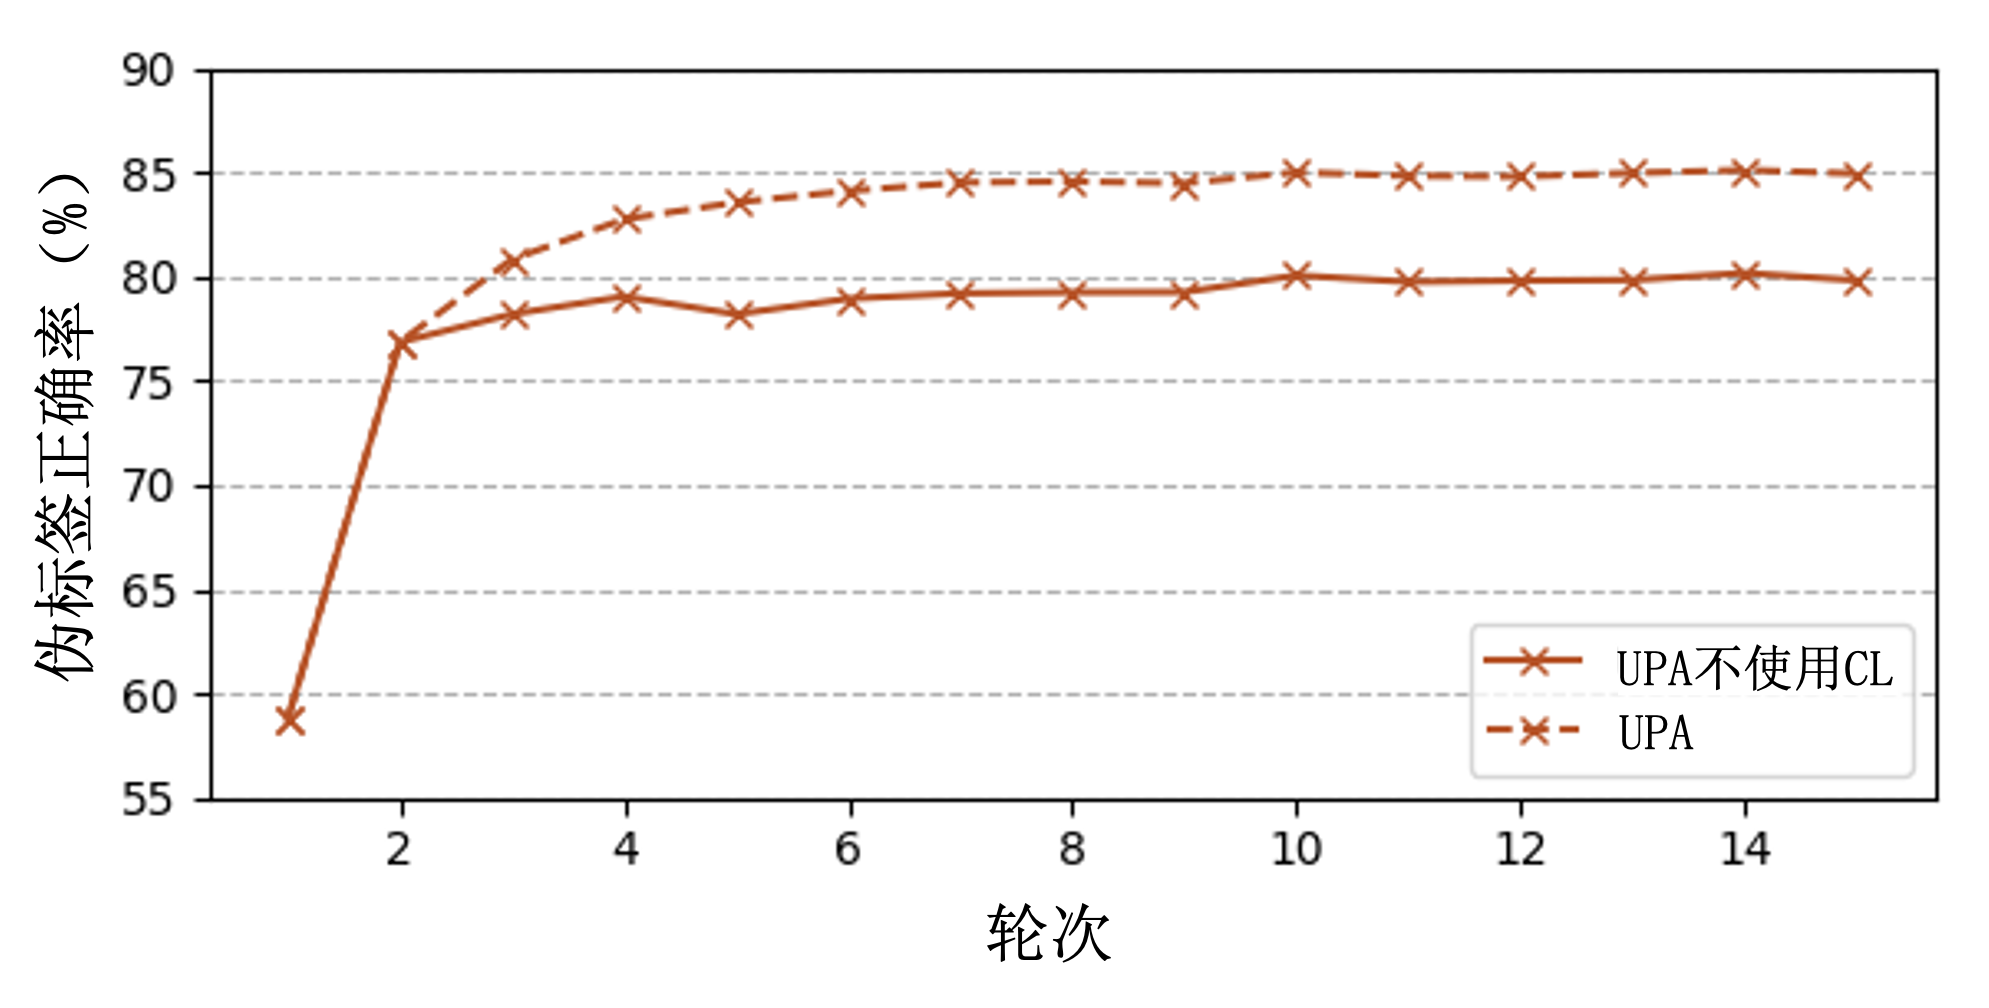
\includegraphics[width=0.55\linewidth]{figures/upa_extracted/cl_pl_acc.png}
  \bicaption[fig:upa_cl_acc]{}{UPA在 VisDA-C 数据集上所选伪标签精度的演化曲线}{Fig.}{Evolution of selected pseudo-label accuracy of UPA on VisDA-C}
\end{figure}

如图~\ref{fig:upa_cl_acc}所示的伪标签准确性演化曲线所示，APS 所选高置信子集 $\mathcal{T}_c$ 上的伪标签精度相比原始伪标签有明显提升。在 VisDA-C 数据集上，这一提升幅度达到 +4.5\%，表明邻居一致性筛选是判别层去噪的有效手段。CACL 的引入进一步放大了这一优势：训练过程中，CACL 促使同类样本在特征空间中聚集，从而持续提升 APS 所选伪标签的精度，形成良性循环。


\begin{table}[!htbp]
    \bicaption[tab:abl_aps]{}{APS 筛选机制在卷积骨干与状态空间骨干上的消融实验}{Table}{Ablation of the APS filtering mechanism on the CNN and the Mamba backbones}
    \vspace{0.5em}\centering\wuhao
    \begin{tabular}{llccc}
    \toprule
    Method & Backbone & APS & Office-Home & VisDA-C \\
    \midrule
    \multicolumn{5}{c}{\textit{基于CNN的方法}} \\
    \midrule
    SHOT~\cite{liang2021source} & ResNet-50/101 & -- & 71.8 & 82.9 \\
    w/ APS    & ResNet-50/101 & \checkmark & 72.7 & 84.2 \\
    \midrule
    \multicolumn{5}{c}{\textit{基于Mamba的方法}} \\
    \midrule
    SHOT~\cite{liang2021source} & VMamba-S & --& 80.3 & 79.9 \\
    w/ APS  & VMamba-S & \checkmark  & 81.2 & 85.4 \\
    \bottomrule
    \end{tabular}
\end{table}


表~\ref{tab:abl_aps}表明，APS 伪标签筛选在两类骨干上均带来正增益，但其作用强度与收益结构存在显著差异。在卷积骨干上，APS 在Office-Home 与 VisDA-C 上分别带来 +0.9\% 与 +1.3\% 的提升；在状态空间骨干上，APS 在 Office-Home 与 VisDA-C 上分别带来 +0.9\% 与 +5.5\% 的提升。



\noindent\textbf{（2）伪标签不确定性估计方式的影响}

\begin{table}[!htbp]
  \bicaption[table:ablation_uncertainty]{}{不同不确定性估计方法的准确率对比}{Table}{Comparison of accuracy with different uncertainty estimation methods.}
  \vspace{0.5em}\centering\wuhao
  % \setlength{\tabcolsep}{8pt}
  \begin{tabular}{lcc}
  \toprule
  方法 & A$\to$P & S$\to$R\\
  \midrule
  Ent（预测熵） & 78.0 & 86.2\\
  Prob（预测概率） & 78.4 & 86.0\\
  Cossim（到聚类中心余弦相似度） & 78.5 & 84.9\\
  APS（K 近邻投票，本方法） & \textbf{79.5} & \textbf{88.7}\\
  \bottomrule
  \end{tabular}
\end{table}

表~\ref{table:ablation_uncertainty}对比了 APS 与三种经典不确定性估计方法在 A$\to$P 与 S$\to$R 任务上的表现。三种基线方法分别为：基于单样本预测概率的 Ent、基于预测概率的 Prob 与基于到聚类中心余弦距离的 Cossim。实验结果显示，基于 $K$ 近邻投票的 APS 在两个任务上均显著优于基线方法。这一优势源于邻居一致性度量能够捕捉特征空间中的局部流形结构，相比单样本不确定性估计具有更强的鲁棒性与判别力。


\begin{table}[!htbp]
  \bicaption[table:ablation_iter]{}{APS 迭代次数的影响}{Table}{Impact of iterative refinement in APS.}
  \vspace{0.5em}\centering\wuhao
  \setlength{\tabcolsep}{8pt}
  \begin{tabular}{lcc}
  \toprule
  迭代次数 & VisDA-C & Office\\
  \midrule
  1 & 87.2 & 89.5\\
  2（本方法） & \textbf{88.7} & \textbf{89.9}\\
  3 & 88.7 & 89.8\\
  \bottomrule
  \end{tabular}
\end{table}

表~\ref{table:ablation_iter}则分析了 APS 中迭代式不确定性估计的收敛轮次。实验表明，引入第二轮迭代后 VisDA-C 与 Office 数据集分别提升 1.5 与 0.4 个百分点；第三轮迭代则无进一步提升甚至略有下降。这说明两轮迭代足以让邻居投票结果收敛，过多的迭代反而可能引入累积误差。


UPA 对四个核心超参数——置信样本筛选比例 $\gamma_{\text{sel}}$、对比温度 $\tau$、K 近邻数 $K$ 与损失权重 $\beta_{\text{CE}}$——在 $\pm 20\%$ 扰动范围内均保持稳定（如图~\ref{fig:param}）。具体而言：$\gamma_{\text{sel}}$ 在 0.5–0.9 范围内变化时，UPA 在 VisDA-C 与 Office 数据集上的精度波动不超过 1 个百分点，展现出良好的工程鲁棒性。$\tau$ 与 $K$ 的敏感性分析同样表明存在一个较宽的舒适区间，便于实际部署时调参。尽管 VisDA-C 数据集因域偏移更严重而对 $\gamma_{\text{sel}}$ 的选择更为敏感，UPA 在该数据集的默认参数设置下仍高于所有对比方法。

\begin{figure*}[!htbp]
  \centering
  \setlength{\tabcolsep}{0pt}
  \subfigure[置信样本筛选比例 $\gamma_{\text{sel}}$]{%
    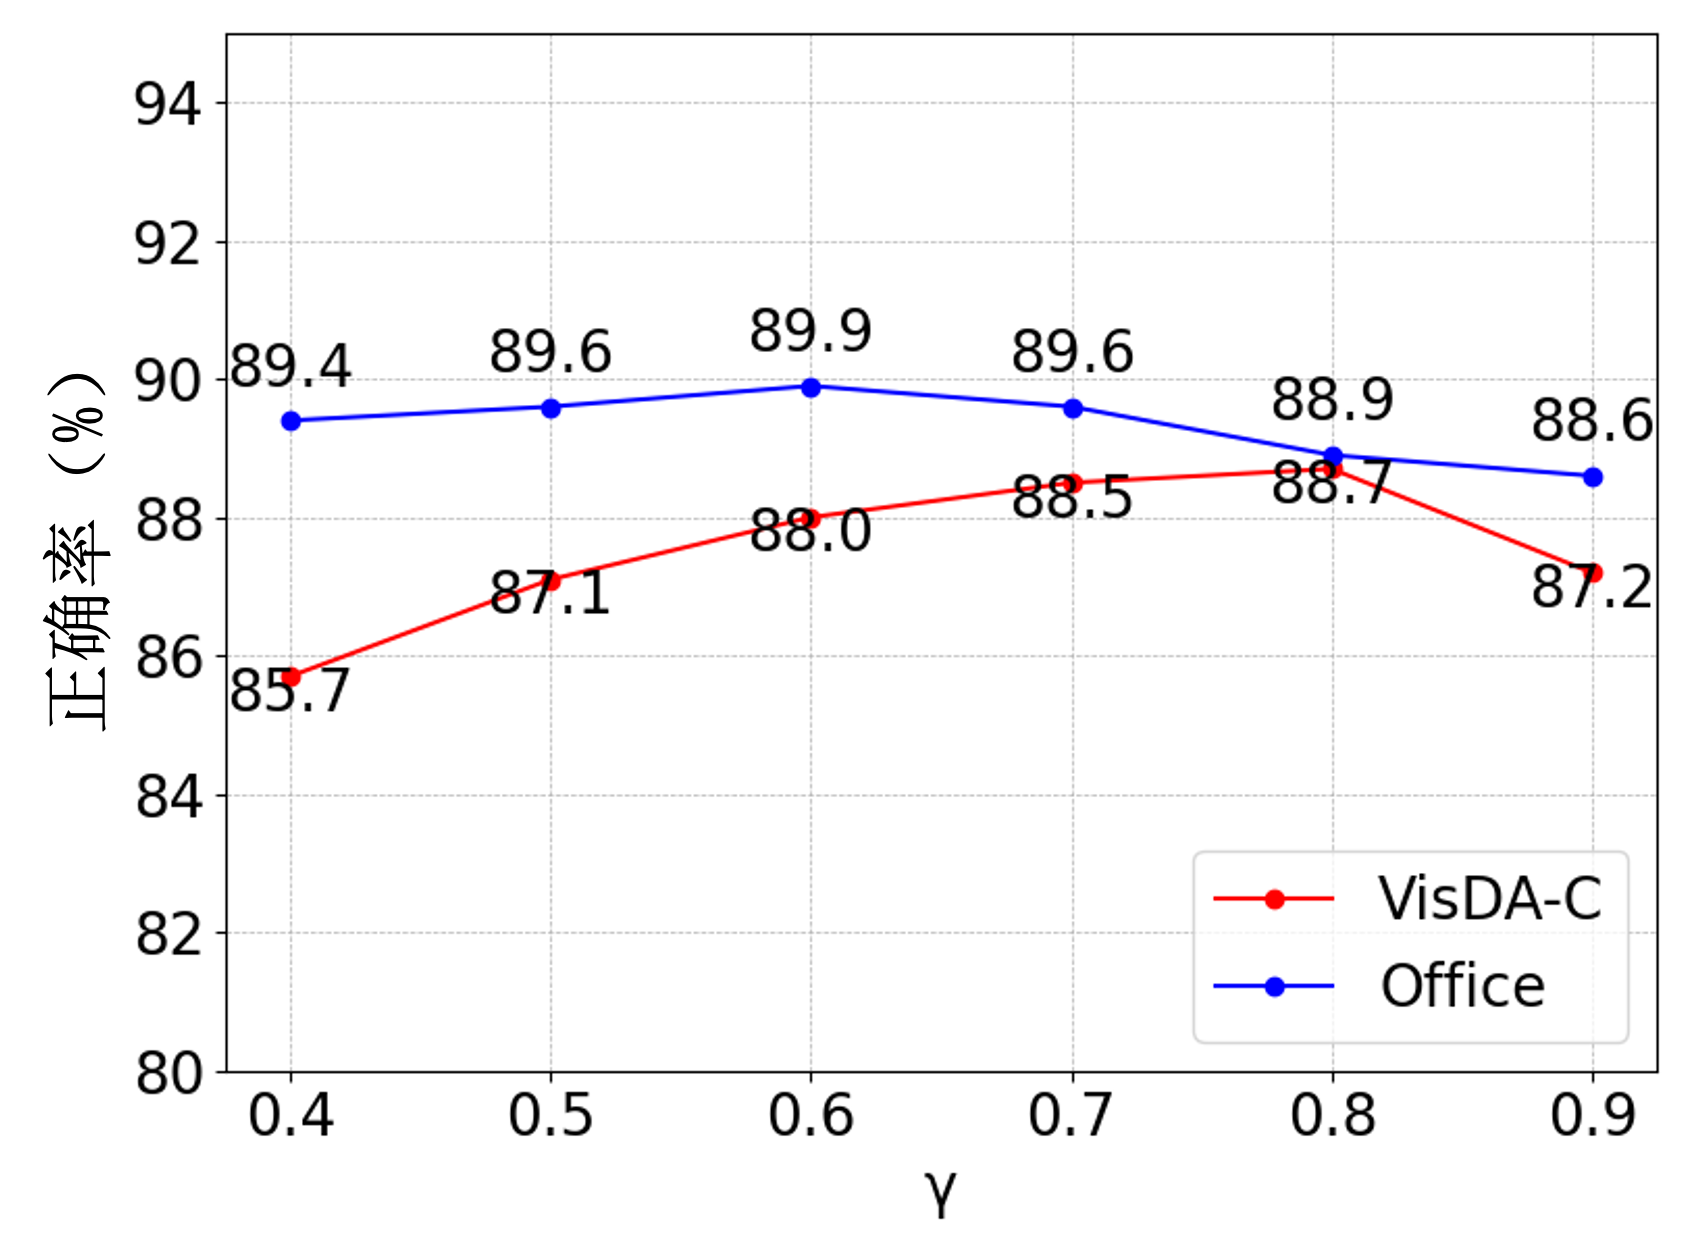
\includegraphics[width=0.3\linewidth]{figures/upa_extracted/re-sel_r_acc.png}
    \label{fig:param_gamma}%
  }\hfill
  \subfigure[对比温度 $\tau$]{%
    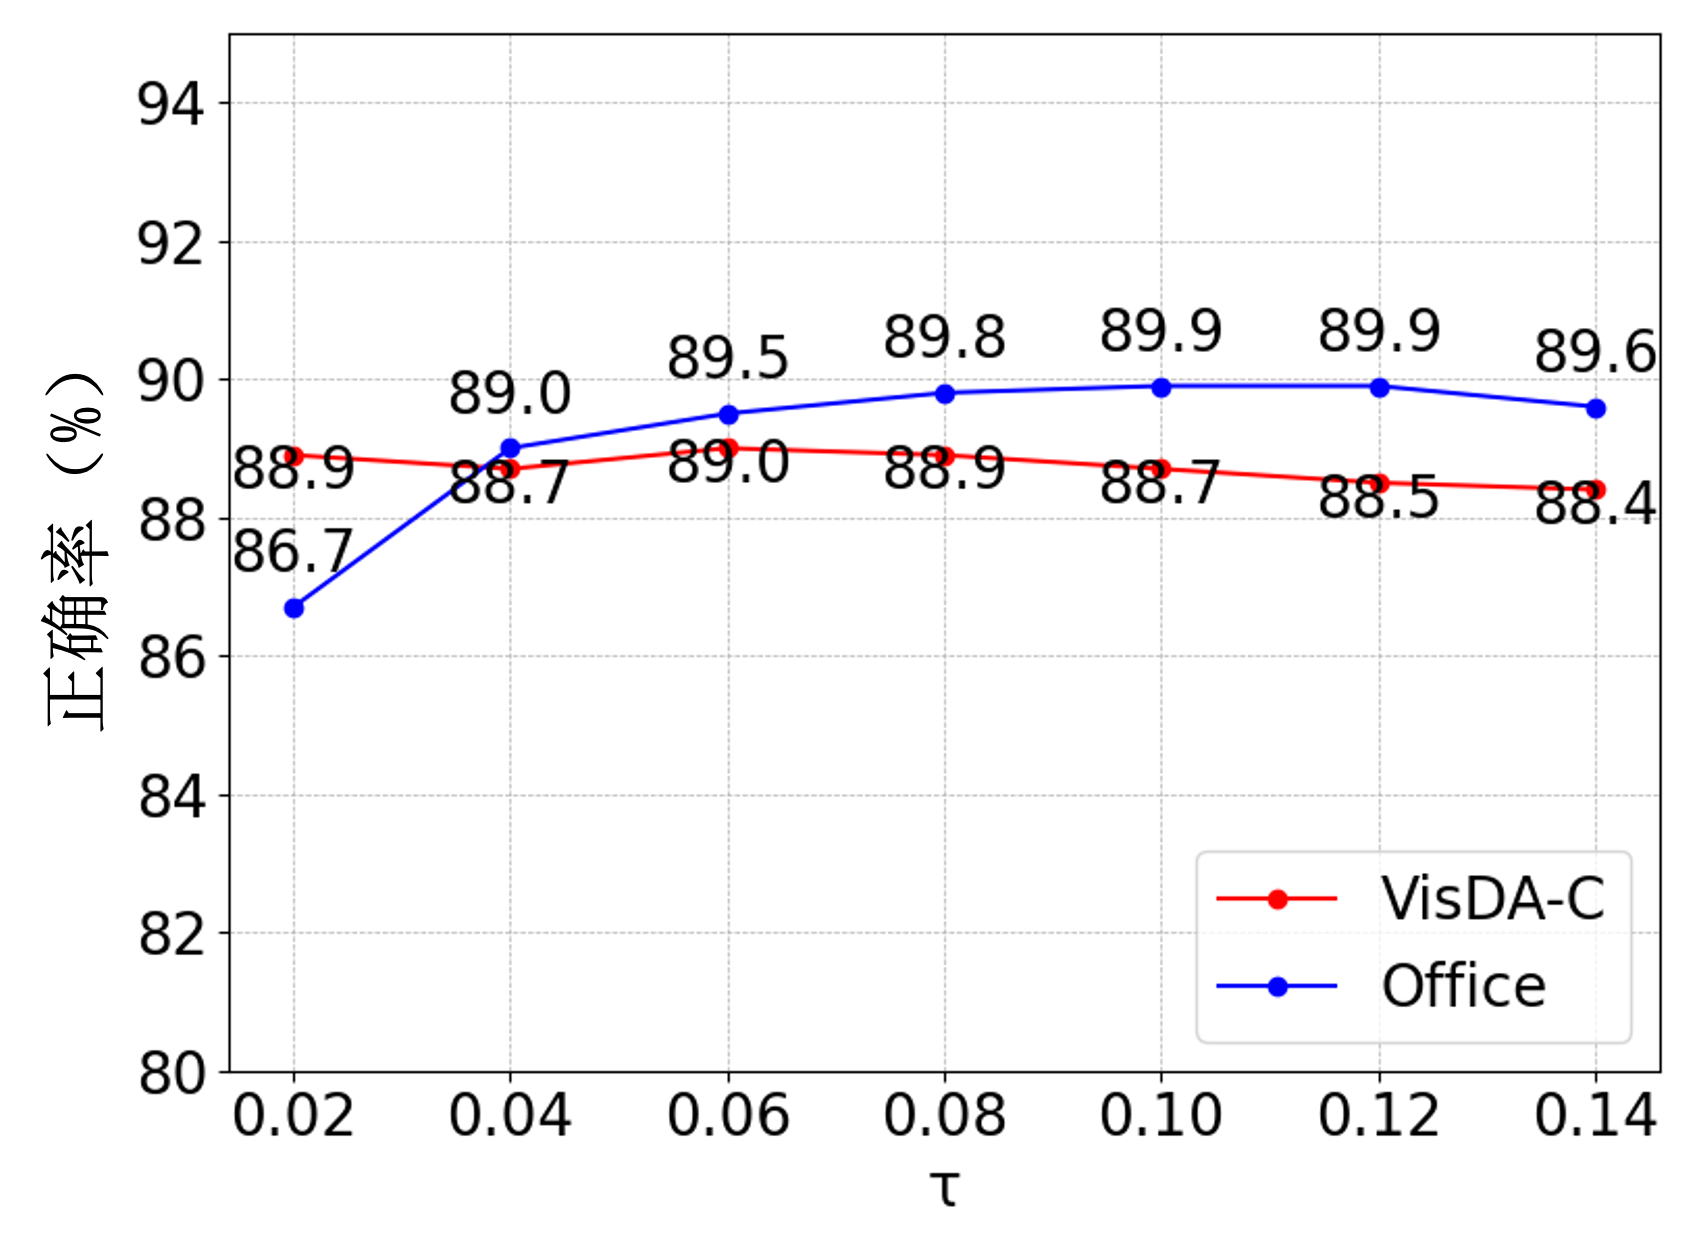
\includegraphics[width=0.3\linewidth]{figures/upa_extracted/re-tau_acc.png}
    \label{fig:param_tau}%
  }\hfill
  \subfigure[近邻数 $K$]{%
    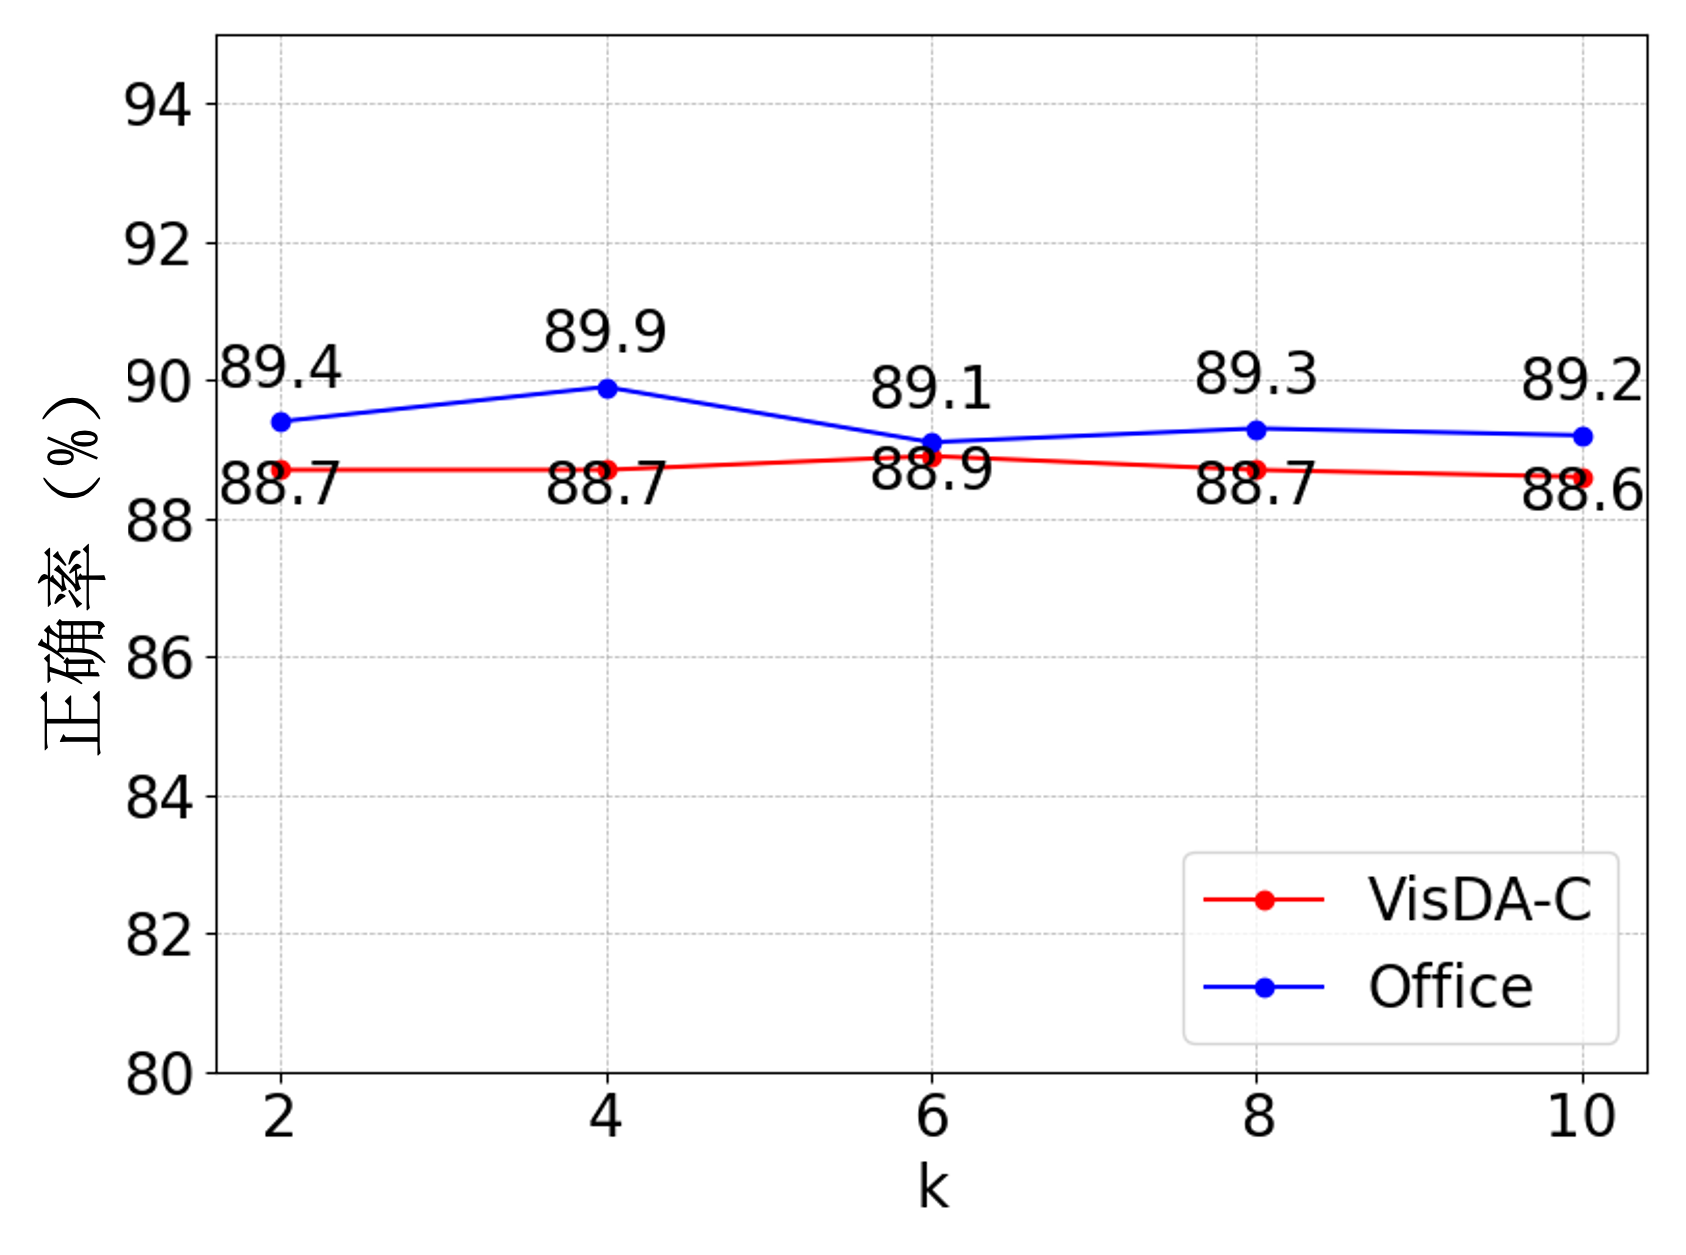
\includegraphics[width=0.3\linewidth]{figures/upa_extracted/re-k_acc.png}
    \label{fig:param_k}%
  }
  \bicaption[fig:param]{}{超参数敏感性分析}{Fig.}{Parameter sensitivity analysis on VisDA-C and Office datasets}
\end{figure*}


\noindent\textbf{（3）表征稳定建模的有效性}


\begin{table}[!htbp]
    \bicaption[tab:ablation_modules]{}{Ch-VSS 与 SCS 模块消融实验}{Table}{Ablation of Ch-VSS and SCS}
    \vspace{0.5em}\centering\wuhao
    \begin{tabular}{ccccc}
    \toprule
    Method & Ch-VSS & SCS & Office-Home & VisDA-C \\
    \midrule
    Baseline$_{\text{S}}$ & -- & -- & 74.4 & 67.3 \\
    Source-S                & -- & \checkmark & 75.3 & 65.6 \\
    \midrule
    Baseline$_{\text{T}}$ & -- & -- & 77.8 & 80.9 \\
    w/ SCS                  & -- & \checkmark & 79.0 & 83.2 \\
    w/ Ch-VSS               & \checkmark & -- & 81.2 & 85.4 \\
    \textbf{SfMamba}        & \checkmark & \checkmark & \textbf{81.7} & \textbf{89.3} \\
    \bottomrule
    \end{tabular}
\end{table}

消融实验,如表~\ref{tab:ablation_modules}所示，验证了两个模块的互补性。对于目标域模型，Ch-VSS 块在 Office-Home 与 VisDA-C 上分别带来 +3.4\% 与 +4.5\% 的增益（Baseline$_{\text{T}}$ $\rightarrow$ $w/$ Ch-VSS），SCS 模块在两基准上分别带来 +1.2\% 与 +2.3\% 的增益（Baseline$_{\text{T}}$ $\rightarrow$ $w/$ SCS）；两模块联合后（$w/$ Ch-VSS $\rightarrow$ SfMamba）在 Office-Home 上带来 +0.5\% 的额外增益，而在 VisDA-C 上带来 +6.1\% 的额外增益，凸显 SCS 在极端域迁移下对序列捷径学习的抑制必要性。
从源域到目标域的端到端增益同样显著：Baseline$_{\text{S}}$ 在 Office-Home 与 VisDA-C 上分别仅取得 +3.4\% 与 +13.6\% 的迁移增益，而完整 SfMamba 在两基准上分别获得 +6.4\% 与 +23.7\% 的迁移增益（均相对 Source-S 基线），验证了 Ch-VSS 与 SCS 在 SFDA 场景下的协同优势。

Grad-CAM 可视化（图~\ref{fig:sfmamba_gradcam}）进一步揭示了 Ch-VSS 与 SCS 的协同作用。在 VisDA-C S$\rightarrow$R 任务上，基线源模型仅能捕捉粗略目标区域；引入 Ch-VSS 后，模型即使在适应前也能更准确识别任务相关区域；完整适应后，SfMamba 的热力图显著聚焦于前景目标。然而当移除 SCS（$w/$ Ch-VSS）时，模型在部分样本上仍表现出不稳定的注意力分布——这表明 Mamba 的序列扫描过程在域迁移下会传播噪声上下文信号，而 SCS 通过打破虚假空间相关性稳定了隐藏状态的演化。
% 图~\ref{fig:sfmamba_cases}的进一步在成功/失败案例上的对比显示，引入 Ch-VSS 一般会带来更聚焦前景目标的注意力图。成功案例中这种定位改进直接贡献于正确预测；失败案例中，模型虽正确关注目标区域，但当视觉相似类别在域迁移下产生重叠特征表征时仍可能误分类。此外，由于 Ch-VSS 通过通道级状态空间建模重塑特征空间，部分样本在适应后可能更接近竞争类别——尤其当细粒度判别性线索被削弱时。整体而言，剩余错误主要源于细粒度语义模糊而非空间注意力错误。

\begin{figure}[!htbp]
    \centering
    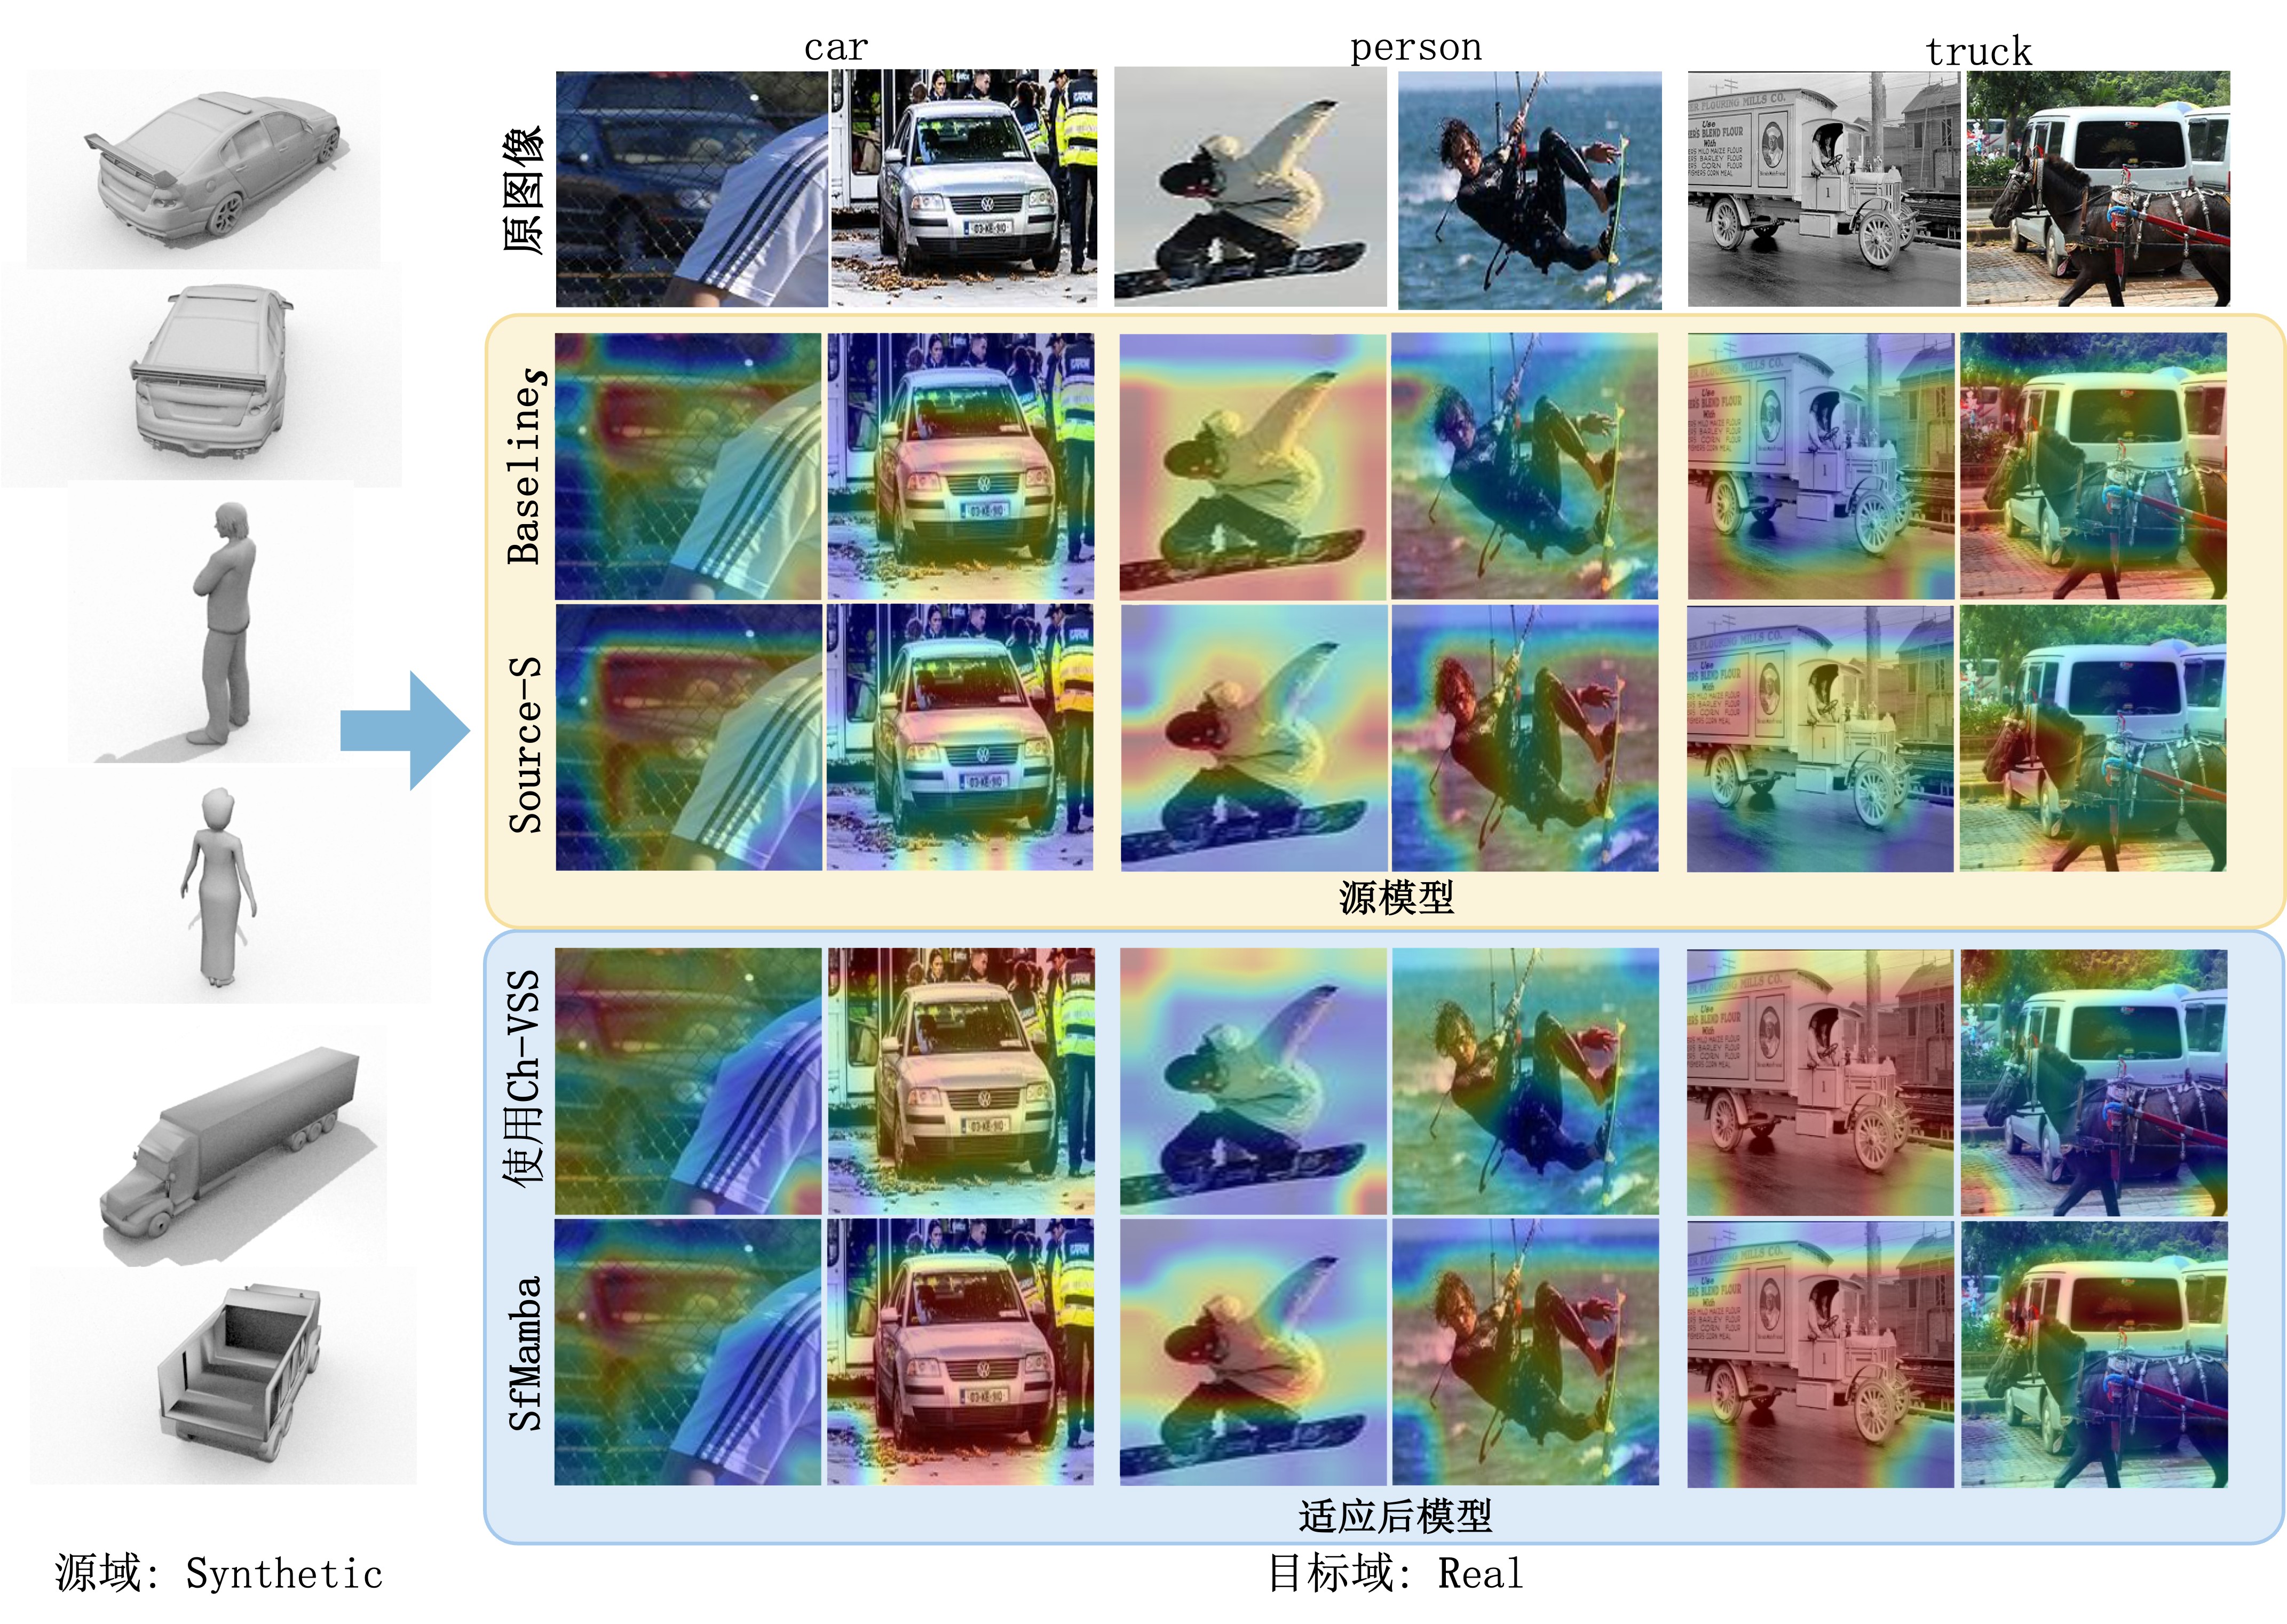
\includegraphics[width=0.9\linewidth]{figures/sfmamba/abl_cam.png}
    \bicaption[fig:sfmamba_gradcam]{}{SCS 模块在 Real 域上的 GradCAM 可视化对比}{Fig.}{GradCAM visualization comparison of the SCS module on the target Real domain of VisDA-C}
\end{figure}

% \begin{figure}[!htbp]
%     \centering
%     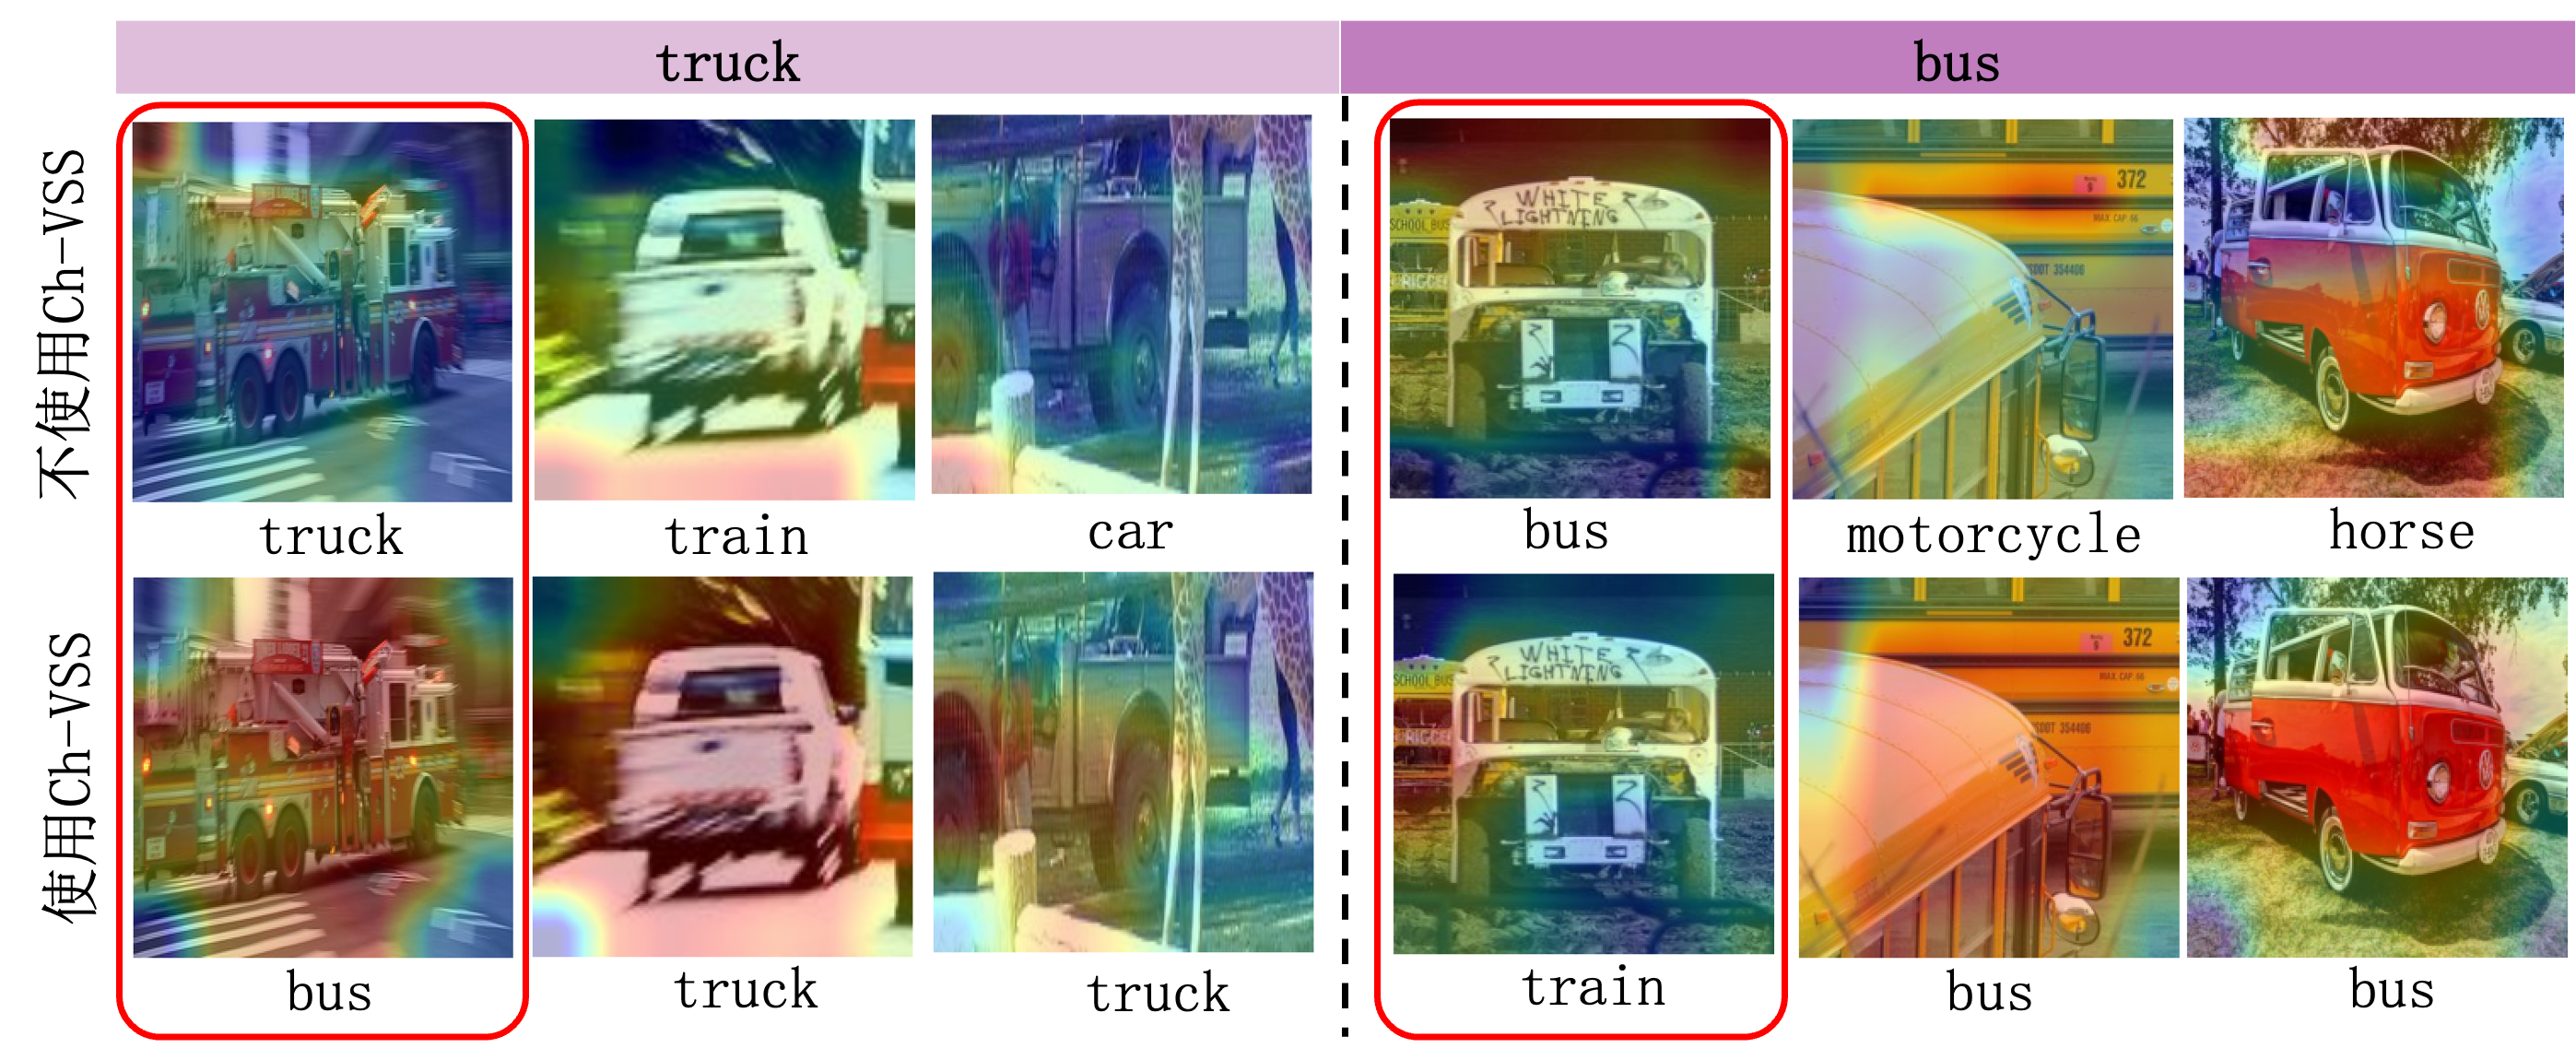
\includegraphics[width=0.8\linewidth]{figures/sfmamba/fail_suc.png}
%     \bicaption[fig:sfmamba_cases]{}{SfMamba 在 VisDA-C 上的典型成功与失败案例}{Fig.}{Representative successful and failure classification cases with SfMamba on VisDA-C}
% \end{figure}


为评估 Ch-VSS 中双向通道扫描设计的有效性，我们对比了 Self-Attention（SA）、Channel Mamba（CM）、Efficient Channel Attention（ECA）与 Convolutional Block Attention Module（CBAM）等代表性通道注意力机制，如表~\ref{tab:abl_attn}所示。实验显示，替代通道机制在 Office-Home 上的平均目标域精度增益至多 0.5\%，而 Ch-VSS 取得显著的 +2.5\% 增益且在所有 12 个迁移任务上均带来提升。
进一步的，为审慎评估双向扫描的充分性，我们进一步设计了 Group-wise Channel Scanning（Ch-Group）变体，将扁平化的 1D 通道特征重塑为宽度 $d$ 的 2D 网格并进行强制行列交叉扫描。如表~\ref{tab:abl_attn}所示，Ch-Group 变体在 A$\rightarrow$C 与 A$\rightarrow$P 两个迁移任务上明显落后于 Ch-VSS（差距分别达 2.5 与 2.4 个百分点），说明有效适应所需的通道依赖已能被 Ch-VSS 的内禀双向扫描充分捕捉，更复杂的强制置换并无必要。
同时，为审慎评估 Ch-VSS 的架构无关性，我们进一步将 Ch-VSS 嵌入到 Agent-DeiT-B、DeiT-B、ConvNeXt-B 与 VMamba-S 四类骨干网络上，详见表~\ref{tab:abl_backbone}。Ch-VSS 在四类骨干上均带来目标域精度提升，其中 VMamba-S 骨干上的提升最为显著（+2.8\% 至 80.2\%），进一步验证了 Ch-VSS 与 Mamba 骨干的协同增益。

\begin{table}[!htbp]
    \bicaption[tab:abl_attn]{}{Ch-VSS 与代表性通道注意力机制在 Office-Home 上的精度对比}{Table}{Source-only / adapted accuracy of Ch-VSS vs.\ alternative channel attention mechanisms on the 12 Office-Home transfer tasks.}
    \vspace{0.5em}\centering\wuhao
    \small
    \setlength{\tabcolsep}{1.5pt}
    \resizebox{\textwidth}{!}{
    \begin{tabular}{l*{12}{c}c}
    \toprule
    注意力机制 & A$\rightarrow$C & A$\rightarrow$P & A$\rightarrow$R & C$\rightarrow$A & C$\rightarrow$P & C$\rightarrow$R & P$\rightarrow$A & P$\rightarrow$C & P$\rightarrow$R & R$\rightarrow$A & R$\rightarrow$C & R$\rightarrow$P & Avg \\
    \midrule
    None       & 62.2/66.6 & 77.9/79.1 & 83.5/82.9 & \underline{75.6}/77.8 & 78.6/82.5 & \underline{81.5}/81.8 & 70.7/75.4 & 56.0/63.3 & 83.5/85.0 & 77.4/81.0 & 59.0/68.0 & \underline{86.2}/88.6 & 74.3/77.7 \\
    SA         & 62.2/\underline{67.6} & 77.8/79.8 & 83.5/85.9 & 74.1/74.0 & 79.9/81.1 & 80.2/82.4 & 69.7/71.7 & 55.5/\underline{65.0} & 83.2/85.5 & 77.0/80.8 & \underline{60.5}/68.2 & 85.7/88.5 & 74.1/77.5 \\
    CM         & \textbf{63.0}/66.3 & \underline{78.2}/79.0 & 84.0/\underline{86.4} & \textbf{76.2}/74.1 & 79.1/\underline{83.4} & 81.0/\underline{84.5} & 69.8/74.1 & 55.6/64.9 & 83.9/\underline{86.2} & \underline{77.8}/80.8 & 59.7/\underline{69.3} & 85.9/\underline{89.2} & 74.5/78.2 \\
    ECA        & 62.8/66.0 & \underline{78.2}/79.3 & 83.7/82.0 & 74.6/75.6 & 79.7/80.9 & 81.0/79.2 & 70.0/74.2 & 56.8/62.3 & 83.4/84.0 & 76.4/80.6 & 60.4/68.2 & 85.5/87.1 & 74.4/76.6 \\
    CBAM       & 62.5/65.1 & 78.0/\underline{81.0} & \underline{84.1}/84.4 & 74.5/76.4 & \underline{80.1}/82.1 & \textbf{81.8}/81.6 & 70.7/74.7 & \textbf{57.2}/63.3 & \underline{84.0}/85.0 & 77.3/\underline{81.1} & 59.9/68.6 & 85.4/88.6 & 74.6/77.7 \\
    \midrule
    Ch-Group   & 62.7/66.2 & \textbf{79.5}/80.8 & \textbf{84.7}/\textbf{86.9} & 75.3/\underline{79.9} & \textbf{80.2}/\textbf{85.0} & 81.2/\textbf{84.8} & \underline{71.8}/\underline{77.1} & \underline{56.9}/\textbf{66.4} & \textbf{84.4}/\textbf{86.6} & \textbf{78.4}/\textbf{81.3} & \textbf{61.9}/\textbf{70.1} & \textbf{86.6}/\textbf{89.7} & \textbf{75.5}/\underline{79.2} \\
    Ch-VSS     & \underline{62.9}/\textbf{68.7} & \textbf{79.5}/\textbf{83.2} & \textbf{84.7}/\textbf{86.9} & 74.4/\textbf{80.4} & \textbf{80.2}/\textbf{85.0} & 81.2/\textbf{84.8} & \textbf{71.9}/\textbf{78.7} & 56.9/\textbf{66.4} & \textbf{84.4}/\textbf{86.6} & \textbf{78.4}/\textbf{81.3} & \textbf{61.9}/\textbf{70.1} & \textbf{86.6}/\textbf{89.7} & \underline{75.3}/\textbf{80.2} \\
    \bottomrule
    \end{tabular}}
\end{table}


\begin{table}[!htbp]
    \bicaption[tab:abl_backbone]{}{Ch-VSS 在四类骨干网络上对 Office-Home 源域 / 适应后精度的影响}{Table}{Effect of the Ch-VSS block on source-only and after-adaptation accuracy across four backbones on Office-Home.}
    \vspace{0.5em}\centering\wuhao
    \small
    \setlength{\tabcolsep}{1.5pt}
    \resizebox{\textwidth}{!}{
    \begin{tabular}{lcc*{12}{c}c}
    \toprule
    骨干网络 & 参数量 (M) & Ch-VSS & A$\rightarrow$C & A$\rightarrow$P & A$\rightarrow$R & C$\rightarrow$A & C$\rightarrow$P & C$\rightarrow$R & P$\rightarrow$A & P$\rightarrow$C & P$\rightarrow$R & R$\rightarrow$A & R$\rightarrow$C & R$\rightarrow$P & Avg \\
    \midrule
    \multicolumn{16}{c}{\textit{源域仅训练}} \\
    \midrule
    \multirow{2}{*}{Agent-DeiT-B} & \multirow{2}{*}{87} & $\times$ & 56.4 & 71.3 & 79.4 & 69.5 & 72.5 & 76.5 & 62.5 & 52.4 & 79.7 & 74.2 & 54.8 & 84.1 & 69.4 \\
                                   &                 & \checkmark  & 61.4 & 77.2 & 81.7 & 67.7 & 75.9 & 77.1 & 66.3 & 55.0 & 81.4 & 73.8 & 57.1 & 83.7 & 71.5 \\
    \midrule
    \multirow{2}{*}{DeiT-B}        & \multirow{2}{*}{86} & $\times$ & 58.2 & 72.2 & 79.3 & 67.7 & 71.8 & 75.6 & 61.4 & 50.4 & 79.1 & 70.7 & 54.6 & 81.6 & 68.6 \\
                                   &                 & \checkmark  & 57.3 & 74.6 & 81.0 & 68.7 & 74.5 & 75.9 & 65.0 & 51.8 & 81.4 & 72.4 & 56.1 & 82.0 & 70.1 \\
    \midrule
    \multirow{2}{*}{ConvNeXt-B}    & \multirow{2}{*}{89} & $\times$ & 61.5 & 76.2 & 82.2 & 71.6 & 76.3 & 79.0 & 69.8 & 55.3 & 82.7 & 77.5 & \underline{62.2} & 85.0 & 73.3 \\
                                   &                 & \checkmark  & \textbf{64.6} & \underline{79.0} & \underline{83.5} & \underline{74.9} & \underline{78.7} & 81.1 & \underline{71.8} & \textbf{57.3} & \textbf{84.5} & 77.9 & \textbf{62.7} & 85.9 & \underline{75.2} \\
    \midrule
    \multirow{2}{*}{Mamba-S}       & \multirow{2}{*}{50} & $\times$ & 62.2 & 77.7 & 83.4 & \textbf{75.2} & \textbf{80.2} & \textbf{82.0} & 71.2 & \underline{57.1} & 83.6 & \underline{78.3} & 61.4 & \underline{86.5} & 74.9 \\
                                   &                 & \checkmark  & \underline{62.9} & \textbf{79.5} & \textbf{84.7} & 74.4 & \textbf{80.2} & \underline{81.2} & \textbf{71.9} & 56.9 & \underline{84.4} & \textbf{78.4} & 61.9 & \textbf{86.6} & \textbf{75.3} \\
    \midrule
    \multicolumn{16}{c}{\textit{适应后}} \\
    \midrule
    \multirow{2}{*}{Agent-DeiT-B} & \multirow{2}{*}{87} & $\times$ & 63.1 & 72.9 & 80.6 & 70.5 & 73.6 & 76.2 & 66.4 & 58.5 & 81.0 & 77.4 & 64.9 & 85.9 & 72.6 \\
                                   &                 & \checkmark  & 64.6 & 81.3 & 84.7 & 74.7 & 80.9 & 80.5 & 74.1 & 62.2 & \underline{85.2} & 78.5 & 66.8 & 88.6 & 76.8 \\
    \midrule
    \multirow{2}{*}{DeiT-B}        & \multirow{2}{*}{86} & $\times$ & 61.0 & 76.3 & 81.6 & 69.8 & 73.6 & 78.6 & 65.8 & 58.8 & 81.4 & 76.6 & 61.8 & 84.8 & 72.5 \\
                                   &                 & \checkmark  & 64.2 & 78.7 & 83.5 & 72.8 & 80.6 & 79.8 & 72.8 & 60.6 & 83.5 & 77.6 & 65.4 & 87.5 & 75.6 \\
    \midrule
    \multirow{2}{*}{ConvNeXt-B}    & \multirow{2}{*}{89} & $\times$ & 62.9 & 76.9 & 83.3 & 75.4 & 78.1 & 78.5 & 72.3 & 60.3 & 82.3 & 76.3 & 62.6 & 82.8 & 74.3 \\
                                   &                 & \checkmark  & \underline{68.1} & \underline{81.5} & \textbf{87.5} & \underline{79.9} & \underline{82.7} & \underline{83.2} & \underline{77.5} & \underline{65.8} & \textbf{86.6} & 80.3 & \textbf{70.2} & \underline{88.7} & \underline{79.3} \\
    \midrule
    \multirow{2}{*}{VMamba-S}      & \multirow{2}{*}{50} & $\times$ & 64.0 & 78.2 & 82.9 & 78.1 & 82.5 & 81.8 & 75.5 & 63.3 & 85.0 & \underline{81.0} & 68.0 & 88.6 & 77.4 \\
                                   &                 & \checkmark  & \textbf{68.7} & \textbf{83.2} & \underline{86.9} & \textbf{80.4} & \textbf{85.0} & \textbf{84.8} & \textbf{78.7} & \textbf{66.4} & \textbf{86.6} & \textbf{81.3} & \underline{70.1} & \textbf{89.7} & \textbf{80.2} \\
    \bottomrule
    \end{tabular}}
\end{table}

% 为考察 Ch-VSS 的最佳应用阶段，我们对比了仅在目标域适应阶段引入 Ch-VSS 与在源域预训练+目标域适应两阶段均引入的两种配置（图~\ref{fig:sfmamba_l_ablation_left}）。仅在目标域适应阶段引入 Ch-VSS（$w/$ Ch-VSS-T）相对基线无任何精度提升；即使在该阶段为 Ch-VSS 块额外添加零初始化的卷积层（$w/$ Ch-VSS-T-Z）以缓解对已训练特征的破坏，精度仍无改善。这表明在源域上预训练 Ch-VSS 模块是必要的——只有经过源域预训练，Ch-VSS 才能习得跨域一致的频域特征重组策略，为目标域适应提供有效的特征基础。


SCS 策略通过 GradCAM 激活值精准识别背景 patch 并施加随机置换。我们对比了三种配置，如表~\ref{tab:abl_scs}所示：不打乱（None）、随机打乱（Random）与选择性打乱（SCS）。在 VisDA-C S$\rightarrow$R 任务上，None、Random、SCS 三种配置分别取得 85.4\%、88.5\% 与 89.3\% 的精度；在 Office-Home 的 A$\rightarrow$C、A$\rightarrow$P、C$\rightarrow$A、P$\rightarrow$A 任务上，SCS 同样取得最佳或并列最佳精度。实验结果揭示两点关键发现：（1）通过 patch 置换打破空间一致性带来了 3.1 个百分点的性能提升（None vs. Random），验证了序列捷径学习的抑制必要性；（2）在随机置换基础上进一步通过激活值精准识别背景 patch 带来额外增益（Random vs. SCS, +0.8 个百分点），表明基于 GradCAM 的选择性打乱能更精准定位捷径学习源头。这些结果证实了所提背景打乱策略通过使模型决策聚焦于前景语义区域，有效增强了跨域鲁棒性。

\begin{table}[!htbp]
    \bicaption[tab:abl_scs]{}{SCS 背景识别策略消融}{Table}{Ablation of SCS background identification}
    \vspace{0.5em}\centering\wuhao
    % \setlength{\tabcolsep}{1pt}
    % \resizebox{.5\textwidth}{!}{
    \begin{tabular}{lccccc}
    \toprule
    \multirow{2}{*}{方法}  & \multicolumn{4}{c}{Office-Home} & VisDA-C \\
    \cmidrule{2-6}
    & A$\rightarrow$C & A$\rightarrow$P & C$\rightarrow$A & P$\rightarrow$A & S$\rightarrow$R \\
    \midrule
    None  & 70.3 & 83.8 & 81.8 & 78.7 & 85.4 \\
    Random & 70.8 & 84.4 & \textbf{82.0} & 78.7 & 88.5 \\
    SCS & \textbf{71.2} & \textbf{84.5} & 81.7 & \textbf{79.0} & \textbf{89.3} \\
    \bottomrule
    \end{tabular}
    % }
\end{table}

% 为进一步辨析 APS 样本筛选与 SCS 在状态空间骨干上的作用边界，我们设计了两者的正交消融实验，如表~\ref{tab:abl_filter}所示。该实验固定 Ch-VSS 模块为开启状态，在 Filter（APS 筛选）与 SCS 两个维度上作 2$\times$2 交叉配置，从而在相同骨干能力下分离出判别层去噪与序列层抑制各自的独立贡献及其交互效应。


% \begin{table}[!htbp]
%     \bicaption[tab:abl_filter]{}{APS 样本筛选与 SCS 的正交消融实验}{Table}{Orthogonal ablation of the APS sample filtering and the SCS strategy}
%     \vspace{0.5em}\centering\wuhao
%     \begin{tabular}{ccccc}
%     \toprule
%     Method & Filter & SCS & Office-Home & VisDA-C \\
%     \midrule
%     Baseline & -- & -- & 80.3 & 79.9 \\
%     $w/$ SCS & -- & \checkmark & 80.9 & \textbf{89.3}\\
%     $w/$ Filter & \checkmark & -- & 81.2 & 85.4\\
%     \textbf{SfMamba} & \checkmark & \checkmark & \textbf{81.7} & \textbf{89.3}\\
%     \bottomrule
%     \end{tabular}
% \end{table}

% 表~\ref{tab:abl_filter}的结果表明，APS 样本筛选与 SCS 在两个基准上呈现出不同性质的作用。在 Office-Home 上，二者具有近似可加的互补效果：单独引入 Filter 带来 +0.9\% 的增益（80.3\% $\rightarrow$ 81.2\%），单独引入 SCS 带来 +0.6\%（80.3\% $\rightarrow$ 80.9\%），二者联合进一步提升至 81.7\%，交互项为 -0.1\%，即两者的收益基本可独立叠加。APS 所解决的伪标签监督信号可靠性问题与 SCS 所解决的序列层空间共现捷径问题，在中等规模偏移下作用于不同的失效模式，因此二者互不替代。

% 而在 VisDA-C 上这一性质发生了显著改变：单独引入 Filter 带来 +5.5\% 的增益（79.9\% $\rightarrow$ 85.4\%），但单独引入 SCS 已带来 +9.4\% 的增益（79.9\% $\rightarrow$ 89.3\%），二者联合的结果 89.3\% 与 SCS 单独使用完全持平，即 Filter 在该基准上未能提供任何超出 SCS 的额外收益。这一现象表明，在合成到真实的极端域偏移下，判别层的伪标签筛选虽能带来可观收益，却远不足以优化 Mamba 骨干的适应性能；Mamba 的适应瓶颈已不在伪标签噪声，而在序列层对背景 patch 空间共现的记忆。SCS 通过置换背景 patch 并施加一致性正则，直接切断了状态转移机制对虚假相关性的累积通路，因而提供了 Filter 所无法替代的增益。

% 该结果从反面验证了本章的核心论点：迁移不确定性的分层抑制需要判别层去噪与骨干级序列增强的协同，缺少任一层次都将导致性能损失；反之，在 Mamba 骨干上，仅有判别层去噪而不引入序列层抑制机制，同样无法达到最优性能。




\noindent\textbf{（4）稳定表征建模超参影响}

\begin{figure}[!htbp]
  \centering
  \setlength{\tabcolsep}{0pt}
  \subfigure[A$\xrightarrow{}$C]{%
    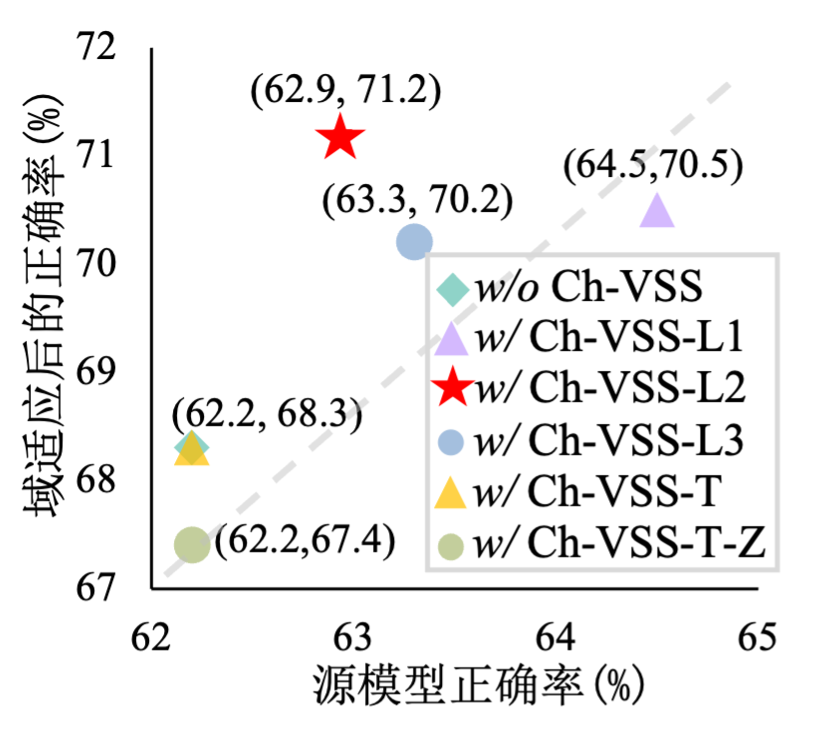
\includegraphics[width=0.4\linewidth]{figures/sfmamba/abl_ch_VSSM_layer_3.png}
    \label{fig:sfmamba_l_ablation_left}%
  }\hfill
  \subfigure[]{%
    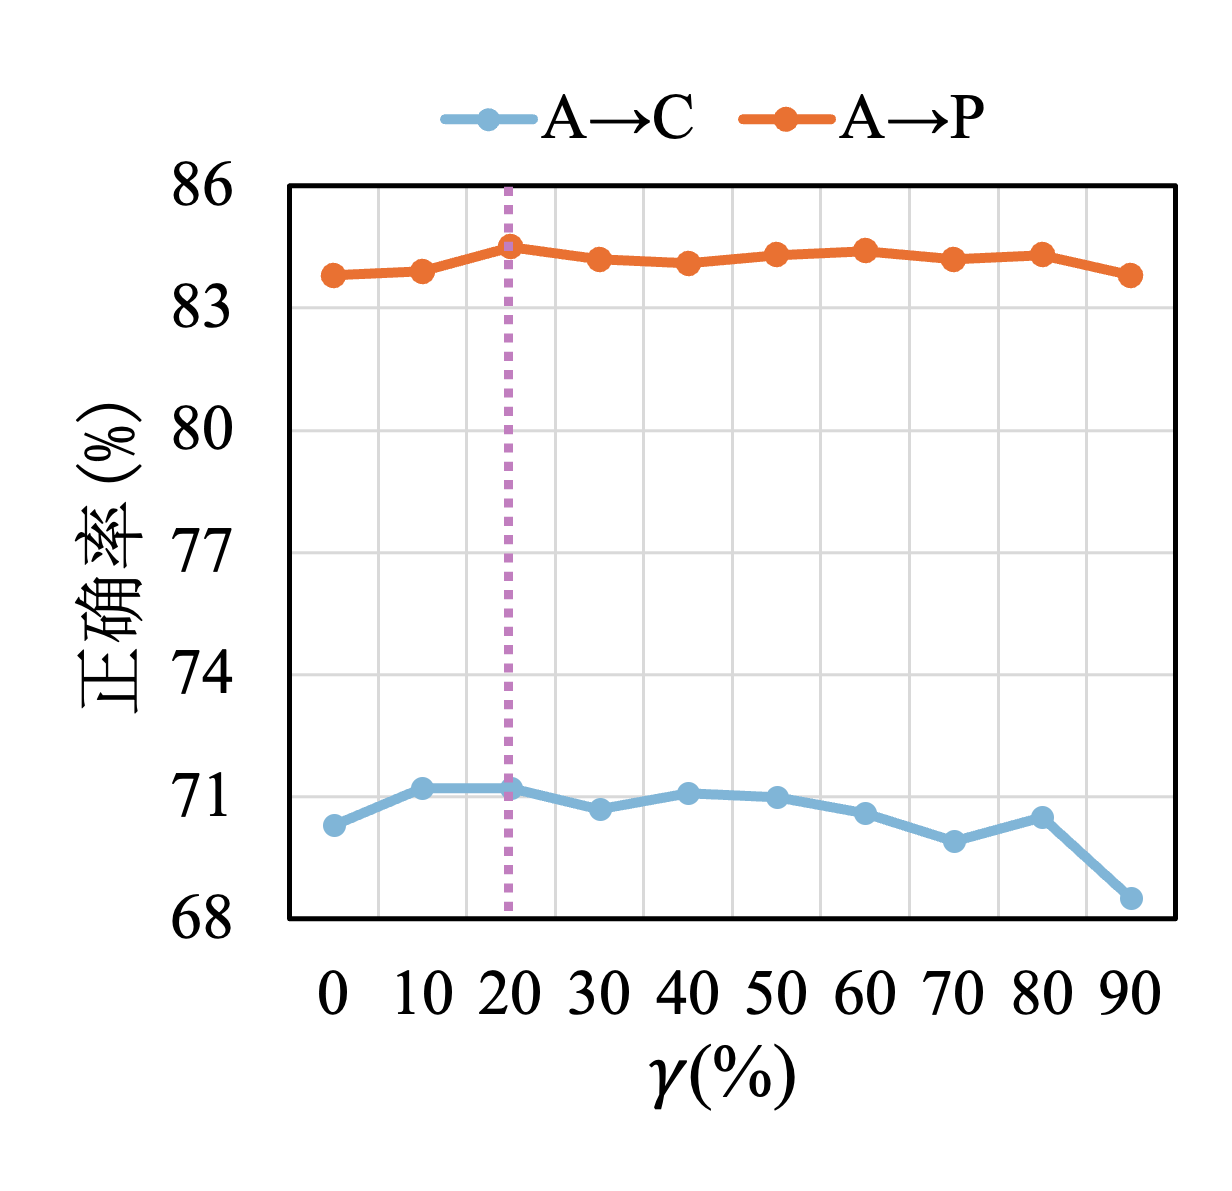
\includegraphics[width=0.4\linewidth]{figures/sfmamba/con_ratio.png}
    \label{fig:sfmamba_l_ablation_right}%
  }
  \bicaption[fig:sfmamba_l_ablation]{}{Ch-VSS 模块数 $L_{\text{vss}}$ 与背景打乱比例 $\gamma_{\text{bg}}$ 的消融}{Fig.}{Ablation on the number of Ch-VSS blocks $L_{\text{vss}}$ and the background shuffle ratio $\gamma_{\text{bg}}$}
\end{figure}

本节考察两个关键超参数：Ch-VSS 块数 $L_{\text{vss}}$ 与 SCS 的背景 patch 比例 $\gamma_{\text{bg}}$。我们记 Ch-VSS 块配置为 Ch-VSS-L$n$，其中 $n$ 表示块数。图~\ref{fig:sfmamba_l_ablation_left} 报告了源域与适应后目标模型在 Office-Home A$\rightarrow$C 任务上的精度。结果显示，引入 Ch-VSS 块始终能提升目标域精度，且 Ch-VSS-L2 配置在目标域上取得最优性能。图~\ref{fig:sfmamba_l_ablation_right} 进一步展示了背景比例 $\gamma_{\text{bg}}$ 对目标精度的影响：当 $\gamma_{\text{bg}}=20$ 时取得最高精度，性能在小 $\gamma_{\text{bg}}$ 值下保持稳定，但 $\gamma_{\text{bg}}$ 过大时显著下降，这与过度打乱会破坏结构化图像内容的预期一致。

% \noindent\textbf{（6） 计算效率}

% 图~\ref{fig:acc_pam} 与表~\ref{tab:efficiency} 联合呈现了 SfMamba 在精度—参数量权衡上的优势。VMamba-S 变体以 58.9M 参数、9.2G FLOPs 取得 Office-Home 81.7\%，超越 DeiT-B 基的 CDTrans/DeSiT（80.5\%，86.6M）；VMamba-T 以 39.0M 参数取得 79.2\%，超越同规模 ViT 与 CNN 基线方法。

% 与 ResNet-101 基的 I-SFDA 相比，VMamba-T 实现减少 4M 参数与 2.4G FLOPs；与 DeiT-B 基的 CDTrans 相比，VMamba-S 减少 32.0\% 参数（27.7M）、47.7\% FLOPs（8.4G），并提升 25.9\% 吞吐量；与 Mamba 基 DATMamba 相比，参数量与 FLOPs 分别减少 38.7M（39.7\%）与 5.8G（38.7\%）。这些结果进一步印证了 SfMamba 在精度—效率双重权衡上的竞争力。

% \begin{figure}[!htbp]
%   \centering
%   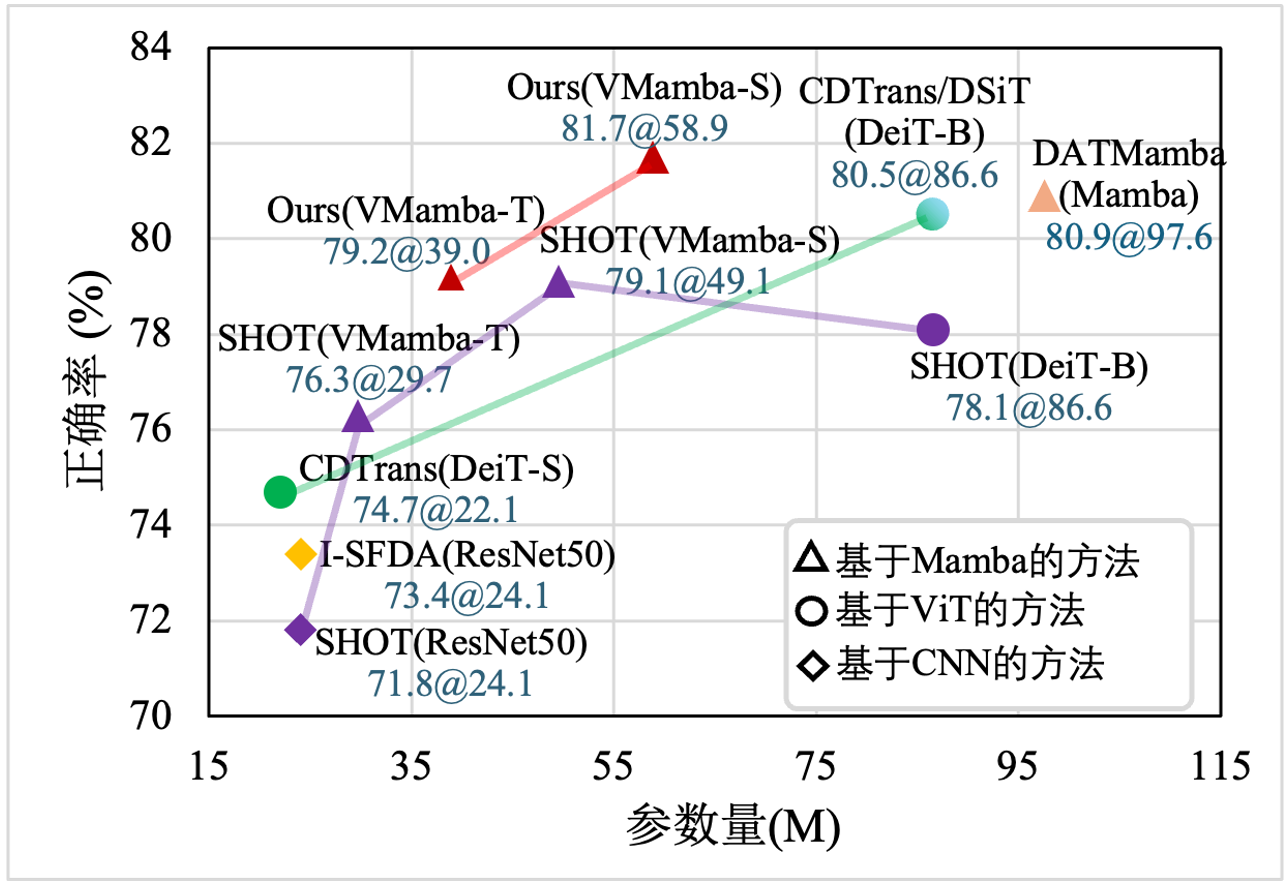
\includegraphics[width=0.7\textwidth]{figures/sfmamba/acc_param.png}
%   \bicaption[fig:acc_pam]{}{不同骨干网络在 Office-Home 上的精度—参数量权衡}{Fig.}{Accuracy vs.\ parameter efficiency across backbones on Office-Home.}
% \end{figure}
% \begin{table}[!htbp]
%     \bicaption[tab:efficiency]{}{SfMamba 在计算效率与精度上的综合对比}{Table}{Computational efficiency comparison of SfMamba}
%     \vspace{0.5em}\centering\wuhao
%     \resizebox{\textwidth}{!}{
%     \begin{tabular}{llcccc}
%     \toprule
%     方法 & 骨干网络 & 参数量 (M) $\downarrow$ & FLOPs (G) $\downarrow$ & 吞吐 (img/s) $\uparrow$ & Office-Home (\%) / VisDA-C (\%) \\
%     \midrule
%     I-SFDA~\cite{mitsuzumi2024understanding} & ResNet-101 & 43.0 & 7.8 & 1094.7 & -- / 88.4 \\
%     SfMamba-T & VMamba-T & 39.0 & 5.4 & 700.9 & 79.2 / 88.5 \\
%     \midrule
%     CDTrans~\cite{xu2022cdtrans} & DeiT-B & 86.6 & 17.6 & 399.5 & 80.5 / 88.4 \\
%     DATMamba~\cite{gao2025datmamba} & Mamba & 97.6 & 15.0 & -- & 80.9 / 88.9 \\
%     \textbf{SfMamba-S} & VMamba-S & \textbf{58.9} & \textbf{9.2} & 502.8 & \textbf{81.7 / 89.3} \\
%     \bottomrule
%     \end{tabular}}
% \end{table}

\FloatBarrier

\section{本章小结}

本章面向无源域适应中源域数据不可访问、目标域无标注所导致的迁移不确定性问题，在统一的伪标签自训练框架下，按不确定性的作用层次展开研究：在判别层，提出基于特征空间邻居结构与类感知对比学习的伪标签去噪方法，从源头抑制噪声在自训练回路中的反复累积，避免引入额外模型；在表征层与序列层，针对状态空间骨干特有的通道建模缺失与空间共现虚假相关，分别以通道维度频率域依赖建模与背景 patch 扰乱稳定跨域表征，以线性复杂度实现高效长程建模。判别层去噪机制在卷积骨干与状态空间骨干上分别得到验证，两个层次在状态空间骨干上叠加使用并取得协同增益。在四个跨域基准上的实验验证了上述不确定性分层抑制机制的有效性。上述结果说明，可靠的目标域监督信号与鲁棒的特征提取机制缺一不可，二者共同构成无源域适应中抑制迁移不确定性的基础。

% Local Variables:% Local Variables:
% TeX-master: "../thesis"
% TeX-engine: xetex
% End:

% !Mode:: "TeX:UTF-8"

\chapter[基于多模态引导和样本挖掘的少监督域迁移]{基于多模态引导和样本挖掘的少监督域迁移}[]
\chaptermark{基于多模态引导和样本挖掘的少监督域迁移}

\label{chap:3}
% 图表与公式编号按章重置并显示为 "章-序"（X-Y）格式，
% 由 book.cls 的 \newcounter{figure}[chapter] / \@addtoreset{equation}{chapter}
% 与 hithesisbook.cls 的 \thefigure / \thetable 定义共同保证；
% 此处不可再调用 \counterwithin，它会把编号改写为 "X.Y" 且全局泄漏到后续章节。

\section{引言}

上一章围绕无监督模型迁移设定，本章进一步讨论在有限监督下如何提升模型迁移性能。
少监督模型迁移涵盖半监督、少样本与主动等多种设定，其核心挑战在于：如何在极为有限的标注预算下最大化监督信号的信息量。本文所称信息最大化，指在给定的监督预算约束下，模型从可获得的监督信号中获取的信息量最大，即训练所得模型对目标域未知标注函数的逼近能力最强。当标注预算极为稀缺时，监督信号的构造面临双重约束：一方面需要在无标注数据中主动挖掘高价值样本，以最小的标注代价换取最大的监督信息增量；另一方面需要借助外部知识源拓展监督信号的覆盖范围与判别可靠性，并使其与任务驱动监督形成假设空间上的互补，最终在学习层面转化为目标模型的判别能力。视觉—语言模型凭借大规模图文对比预训练积累了丰富的开放语义判别能力，其预测不依赖源域分布，能够为稀缺标注场景下的跨域迁移提供与任务驱动监督互补的语义判断信号。然而，如何建立视觉—语言模型与源模型在信息驱动采样与双向深度协同层面的严谨理论框架，仍是一个尚未解决的关键问题。

针对上述挑战，本章围绕稀缺监督条件下的信息最大化问题，沿样本筛选与跨模型协同两个角度协同推进。在样本筛选层面，借助信息驱动的主动采样机制在无标注目标域中挖掘高价值样本，以最小的标注代价换取最大的监督信息增量；在跨模型协同层面，借助视觉—语言模型的开放语义判别能力实现与源模型的双向深度协同，在避免视觉—语言模型丧失泛化能力的同时实现两类监督信号的互补融合。为建立理论指导，本章推导了少监督场景下的协作风险上界，揭示了双假设空间下的样本覆盖、视觉—语言模型的目标域风险与跨模型对齐损失三个关键因素的协同优化目标，为后续模块设计提供可量化的优化目标。实验在闭集与开放集两种设定下均取得当前最优性能，并展示了所提方法在训练效率与额外开销上的工程实用性。

本章工作可归纳为以下三点：
\begin{enumerate}
    \item 少监督场景协作风险上界理论：建立面向稀缺标注条件下的协作风险上界理论分析，明确主动样本选择、视觉—语言模型适应与跨模型对齐三者的协同优化目标。
    \item DAMF 双主动学习框架：首次将视觉—语言模型引入稀缺标注条件下的模型迁移框架，通过双向蒸馏机制实现其与目标模型的有效交互，在闭集与开放集两种设定下均取得当前最优性能，且训练阶段仅引入可忽略的额外参数量（+0.002M）与显存开销（+0.48 GB）。
    \item 实验验证与综合分析：在 Office、Office-Home、VisDA-C 与 miniDomainNet 四个跨域基准的闭集与开放集两种设定下均取得当前最优性能；闭集与开放集场景下的性能提升均高于现有方法，验证了样本筛选与跨模型协同设计的有效性；在部分跨域任务上，所提方法的精度高于依赖源域数据访问的域适应 与主动域适应方法，说明多模态融合在低资源场景下具备补充价值。
\end{enumerate}

\section{基于多模态基础模型引导的主动域适应方法}

\label{sec:chap3_damf}

在无源主动域适应（Source-Free Active Domain Adaptation, SFADA）设定中，源域模型 $\theta_s$ 在带标签的源域数据集 $\mathcal{S}=\{(x_i,y_i)\}_{i=1}^{n_s}\in(\mathcal{X}^{n_s},\mathcal{Y}_s)$ 上预训练得到。给定无标签目标域数据集 $\mathcal{T}=\{x_i'\}_{i=1}^{n_t}\in\mathcal{X}^{n_t}$（含 $C_t$ 个类别），SFADA 的目标是在标注预算 $B$（$B=|\mathcal{T}_q|=\rho|\mathcal{T}|$，$\rho\in(0,1)$）的约束下，通过主动查询策略 $\pi$ 从 $\mathcal{T}$ 中选取子集 $\mathcal{T}_q$ 进行人工标注，最终使目标模型 $\theta_t$（由 $\theta_s$ 初始化）在目标域上的期望风险最小化。借鉴文献~\cite{wang2023mhpl,chu2022denoised}，本章采用单批次一次性查询策略，即所有标注样本 $\mathcal{T}_q$ 在训练开始前一次性选定。源域数据 $\mathcal{S}$ 在适应阶段不可访问。

目标模型对类别 $k$ 的预测概率定义为 $p_T^{(k)}(x)=\theta_t^{(k)}(x)$。本章同时考虑两种设定：（1）闭集设定，$\mathcal{Y}_s=\mathcal{Y}_t$，$C_s=C_t$；（2）开放集设定，$\mathcal{Y}_s\subset\mathcal{Y}_t$，需要在识别 $C_s$ 个已知类别的同时拒绝其余 $|\mathcal{Y}_u|=|\mathcal{Y}_t|-|\mathcal{Y}_s|$ 个未知类别（统一标记为 ``unknown''）。

为利用跨模态先验，本章引入 ViL 模型 $\theta_v$ 作为辅助监督源。设 $\mathbf{I}=\phi(x)$ 为 ViL 图像编码器提取的图像特征，文本嵌入通过类别级可学习 prompt $\{V_k\}_{k=1}^{C}$ 生成，每个 prompt 结构为 $V_k=\{v_1,v_2,\cdots,v_m,c_k\}$，其中 $c_k$ 为类别名称，初始化模板为 ``a photo of a [$c_k$]''。文本嵌入 $\mathbf{w}_k=\mathrm{Enc}_t(V_k)$ 由冻结的文本编码器生成，则 ViL 模型的预测概率为：
\begin{equation}
p_V^{(k)}(x) = \theta_v(x; V_k) = \frac{\exp(\mathrm{sim}(\mathbf{I}, \mathbf{w}_k)/\tau)}{\sum_{i=1}^{C}\exp(\mathrm{sim}(\mathbf{I}, \mathbf{w}_i)/\tau)},
\label{eq:vil_pred}
\end{equation}
其中 $\mathrm{sim}(\cdot,\cdot)$ 为余弦相似度，$\tau$ 为可学习的温度参数。在整个适应过程中，ViL 模型的图像和文本编码器均被冻结，仅优化类别 prompt 以激活其任务感知能力。

% 为便于本章后续对符号的统一引用，本节将涉及的关键符号汇总于表~\ref{tab:chap3_symbols}。

% \begin{table}[!htbp]
%     \bicaption[tab:chap3_symbols]{}{本章关键符号及其定义}{Table}{Key symbols and their definitions}
%     \vspace{0.5em}\centering\wuhao
%     \setlength{\tabcolsep}{8pt}
%     \resizebox{\textwidth}{!}{
%     \begin{tabular}{ll}
%         \toprule
%         符号 & 含义 \\
%         \midrule
%         $\mathcal{S}$ / $\mathcal{T}$ & 源域 / 目标域数据 \\
%         $\mathcal{X}$ / $\mathcal{Z}$ & 样本空间 / ViL 特征空间，其中 $\mathcal{Z}=\{z\mid z=\phi(x),\forall x\in\mathcal{T}\}$ \\
%         $\mathcal{Y}_{s/t}$ / $C_{s/t}$ & 源 / 目标类别空间 / 类别数 \\
%         $n_{s/t}$ & 源 / 目标样本数 \\
%         $x$ / $y$ & 样本 / 标签 \\
%         $P$ / $Q$ & 目标域 / 源域分布 \\
%         $\hat{P}$ / $\hat{Q}$ / $\widetilde{Q}$ & $\mathcal{T}$ / $\mathcal{D}_l$ / $\mathcal{T}_q$ 的经验分布，其中 $\mathcal{D}_l=\mathcal{S}\cup\mathcal{T}_q$ \\
%         $f_{P/Q}$ & 目标 / 源标注函数 $\mathcal{X}\to\mathcal{Y}$ \\
%         $f'_P$ & ViL 标注函数 $\mathcal{Z}\to\mathcal{Y}$ \\
%         $\theta_{s/t/v}$ & 源模型 / 目标模型 / ViL 模型 \\
%         $\pi$ / $B$ / $\rho$ & 主动采样策略 / 标注预算 / 采样比例（$B=\rho|\mathcal{T}|$） \\
%         $\mathcal{T}_q$ & 主动标注的目标样本子集 \\
%         $\mathcal{H}$ / $\mathcal{G}$ & $k$-Lipschitz / $k_V$-Lipschitz 假设空间 \\
%         $\mathcal{H}_\epsilon$ & 满足 $\mathcal{S}\cup\mathcal{T}_q$ 上 $L(h,f_Q)\le\epsilon$ 的假设子集 \\
%         $\mathfrak{R}_{n_t}(\mathcal{H})$ & $\mathcal{H}$ 上的期望 Rademacher 复杂度 \\
%         $\eta_{\mathcal{G}}$ & 协同假设空间下的理想最大误差 \\
%         $L$ / $\mathcal{L}_{\mathcal{D}}(h,h')$ / $M$ & 对称 $\mu$-Lipschitz 有界损失 / 经验风险 / 损失上界 $0\le L\le M$ \\
%         $d_{\mathcal{U}}$ / $d_X$ / $d_Z$ / $d_Y$ & 距离函数 $d_{\mathcal{U}}:\mathcal{U}\times\mathcal{U}\to\mathbb{R}_{+}$，分别定义于 $\mathcal{U}=\mathcal{X},\mathcal{Z},\mathcal{Y}$ 上 \\
%         $\phi$ & ViL 图像编码器 $\mathcal{X}\to\mathcal{Z}$ \\
%         $\mathbf{I}$ & ViL 图像特征，$\mathbf{I}=\phi(x)$ \\
%         $c_k$ / $V_k$ / $\mathrm{Enc}_t(\cdot)$ / $\mathbf{w}_k$ & 类别 $k$ 的名称 / 可学习 prompt 模板 / ViL 文本编码器 / 文本嵌入 $\mathbf{w}_k=\mathrm{Enc}_t(V_k)$ \\
%         $\tau$ & ViL 模型的可学习温度参数 \\
%         \bottomrule
%     \end{tabular}}
% \end{table}

\subsection{多模型协作风险上界理论}

基于单模型基于差异的主动域适应（DBALDA）~\cite{mathelin2022discrepancy} 理论框架，本节推导了多模型协同 SFADA 的协作风险上界。

设假设空间 $\mathcal{H}$ 由 $k$-Lipschitz 函数组成：$\forall h\in\mathcal{H},\forall x,x'\in\mathcal{X}: d_Y(h(x),h(x'))\leq k\cdot d_X(x,x')$。类似地，ViL 假设空间 $\mathcal{G}$ 由 $k_V$-Lipschitz 函数组成。损失函数 $L:\mathcal{Y}\times\mathcal{Y}\to\mathbb{R}^+$ 对称、$\mu$-Lipschitz、有界（$0\leq L(y,y')\leq M$），且满足三角不等式。ViL 图像编码器 $\phi:\mathcal{X}\to\mathcal{Z}$ 为确定性映射。

引理 3.1（UDA设定下目标风险上界~\cite{mathelin2022discrepancy}）。给定标注集合 $\mathcal{D}_l=\mathcal{S}\cup\mathcal{T}_q$，定义 $\mathcal{H}$ 在 $\mathcal{S}\cup\mathcal{T}$ 上的理想最大误差：
\begin{equation}
\eta_{\mathcal{H}} = \min_{h\in\mathcal{H}}\max_{x\in\mathcal{S}\cup\mathcal{T}}\big[L(h(x), f_Q(x)) + L(h(x), f_P(x))\big].
\label{eq:eta_H}
\end{equation}
则对任意 $\epsilon\geq\eta_{\mathcal{H}}$，$h\in\mathcal{H}_\epsilon$ 及 $\delta>0$，以至少 $1-\delta$ 的概率：
\begin{equation}
L_P(h,f_P) \leq L_{\hat{Q}}(h,f_Q) + \underbrace{2k\mu\frac{1}{n_t}\sum_{x'\in\mathcal{T}}d_X(x',\mathcal{D}_l)}_{\text{覆盖项}} + (2\epsilon+\eta_{\mathcal{H}}) + 2\mu\mathfrak{R}_{n_t}(\mathcal{H}) + \sqrt{\frac{M^2\log(1/\delta)}{2n_t}}.
\label{eq:uda_bound}
\end{equation}

引理 3.2（SFDA设定下目标风险上界）。由于源域数据 $\mathcal{S}$ 不可访问，将式 \eqref{eq:uda_bound} 中的标注集合 $\mathcal{D}_l$ 替换为 $\mathcal{T}_q$，并将理想最大误差限制在目标域 $\mathcal{T}$ 上：
\begin{equation}
\eta'_{\mathcal{H}} = \min_{h\in\mathcal{H}}\max_{x\in\mathcal{T}}\big[L(h(x), f_Q(x)) + L(h(x), f_P(x))\big],
\end{equation}
则以至少 $1-\delta$ 的概率，对任意 $h\in\mathcal{H}'_{\epsilon}$ 及 $\epsilon'\geq\eta'_{\mathcal{H}}$：
\begin{equation}
L_P(h,f_P) \leq L_{\tilde{Q}}(h,f_Q) + 2k\mu\frac{1}{n_t}\sum_{x'\in\mathcal{T}}d_X(x',\mathcal{T}_q) + (2\epsilon'+\eta'_{\mathcal{H}}) + 2\mu\mathfrak{R}_{n_t}(\mathcal{H}) + \sqrt{\frac{M^2\log(1/\delta)}{2n_t}},
\label{eq:sfda_bound}
\end{equation}

引理 3.3（跨空间Lipschitz迁移）\label{cross_lip_trans} 对任意 $x'\in\mathcal{T},x\in\mathcal{T}_q$：
\begin{equation}
\big|L(f_P(x'),f'_P(x')) - L(f_P(x),f'_P(x))\big| \leq \mu\big[kd_X(x',x) + k_Vd_Z(\phi(x'),\phi(x))\big].
\label{eq:cross_lipschitz}
\end{equation}

定理 3.4（协同SFADA风险上界）\label{theorem_coll} 设 $f'_P$ 为 $\mathcal{Z}\to\mathcal{Y}$ 的 ViL 标注函数，定义 $\mathcal{G}$ 关于 $\mathcal{H}$ 在 $\mathcal{T}$ 上的理想最大误差：
\begin{equation}
\eta_{\mathcal{G}} = \min_{g_V\in\mathcal{G}}\max_{x\in\mathcal{T}}\big[L(h(x),g_V(x)) + L(g_V(x),f'_P(x))\big].
\end{equation}

则以至少 $1-\delta$ 的概率：
\begin{align}
L_P(h,f_P) \leq {} & L_{\tilde{Q}}(f_P,f'_P)
 + \underbrace{\mu\frac{1}{n_t}\sum_{x'\in\mathcal{T}}\big[kd_X(x',\mathcal{T}_q) + k_Vd_Z(\phi(x'),\mathcal{T}_q)\big]}_{\text{覆盖项}} \notag\\
& + \eta_{\mathcal{G}} + 2\mu\big[\mathfrak{R}_{n_t}(\mathcal{H}) + \mathfrak{R}_{n_t}(\mathcal{G}\circ\phi)\big]
 + 2\sqrt{\frac{M^2\log(3/\delta)}{2n_t}}.
\label{eq:collab_bound}
\end{align}


\textit{注3.1} 定理 3.4 揭示了降低协同 SFADA 风险上界的三个关键因素：（1）双假设空间
（$\mathcal{X}$ 与 $\mathcal{Z}$）下的样本覆盖项；（2）ViL 模型的目标域误差 $L(g(x),f'_P
(x))$；（3）跨模型对齐损失 $L(h(x),g_V(x))$。本方法通过 DFSelector、APT 和 ADL 三个模块分别
针对上述三项进行优化。定理3.4的公式推导见附录~\ref{app:theorem_3_4_proof}。



\begin{table}[!htbp]
    \bicaption[tab:chap3_bound_module]{}{式~\eqref{eq:collab_bound} 中各项与 DAMF 算法的对应关系}{Table}{Correspondence between the terms of Eq.~\eqref{eq:collab_bound} and the DAMF modules}
    \vspace{0.5em}\centering\wuhao
    % \setlength{\tabcolsep}{6pt}
    % \resizebox{\textwidth}{!}{
    % \begin{tabular}{l|l|l|l}

    \vspace{0.5em}\centering\zihao{-5}
    \setlength{\tabcolsep}{5pt}
    \renewcommand{\arraystretch}{1.2}
    \begin{tabularx}{\textwidth}{@{}p{0.30\textwidth}p{0.32\textwidth}p{0.26\textwidth}@{}}
    \toprule
    上界成分 & 理论含义 & 对应模块 \\
    \midrule
    $L_{\tilde{Q}}(f_P,f'_P)$ & ViL 标注函数与真实标注函数在标注集上的经验不一致度 & APT \\
    $\big[kd_X(\cdot,\mathcal{T}_q)+k_Vd_Z(\cdot,\mathcal{T}_q)\big]$ & 标注集在 $\mathcal{X}$ 与 $\mathcal{Z}$ 双空间下的代表性不足 & DFSelector \\
    $L(h(x),g_V(x))$（$\eta_{\mathcal{G}}$ 内） & 目标模型与 ViL 模型在目标域上的预测分歧 & ADL 的 $\theta_t\leftarrow\theta_v$ 路径 \\
    $L(g_V(x),f'_P(x))$（$\eta_{\mathcal{G}}$ 内） & ViL 模型自身在目标域上的标注误差 & APT + ADL 的 $\theta_v\leftarrow\theta_t$ 路径 \\
    \bottomrule
    \end{tabularx}
    % }
\end{table}

% 需要强调的是，$\eta_{\mathcal{G}}$ 的两个子项并非由单一模块各自独立承担，而是构成一组互补的耦合目标：仅优化 $L(h(x),g_V(x))$ 而不优化 $L(g_V(x),f'_P(x))$，会使 ViL 模型作为教师时本身携带目标域偏置，从而把噪声对齐进目标模型；仅优化 $L(g_V(x),f'_P(x))$ 而不优化 $L(h(x),g_V(x))$，则 ViL 模型与目标模型在无标注样本上仍各行其是，互补语义无法传递到目标模型。ADL 的双向不对称设计正是针对这一耦合关系：$\theta_t\leftarrow\theta_v$ 路径以硬标签形式压减 $L(h(x),g_V(x))$，$\theta_v\leftarrow\theta_t$ 路径以软标签形式在压减 $L(g_V(x),f'_P(x))$ 的同时维持 ViL 模型的类别间关系结构，二者交替执行。表~\ref{tab:ablation_loss} 给出的消融数据与此一致：仅启用 ADL 的目标模型分支（$\mathcal{L}_T$）时闭集精度为 79.4\%，加入 ViL 分支（$\mathcal{L}_V$）后升至 82.9\%，而两者与 APT 同时启用时达到 84.8\%，说明三项优化目标只有联合优化才能取得理论所预示的收益。定理3.4的公式推导见附录~\ref{app:theorem_3_4_proof}。

% \subsection{总体框架}

DAMF 的总体框架如图~\ref{fig:damf_framework}所示。基于定理 3.4 揭示的降低协同 SFADA 风险上界的三个关键因素，DAMF 分别设计了 DFSelector、APT 与 ADL 三个模块，对应关系如表~\ref{tab:chap3_bound_module}所示，依次在训练流程中承担“标注选取 — 提示微调 — 双向蒸馏”的角色，形成端到端的协同适应框架。

\begin{figure}[!htbp]
    \centering
    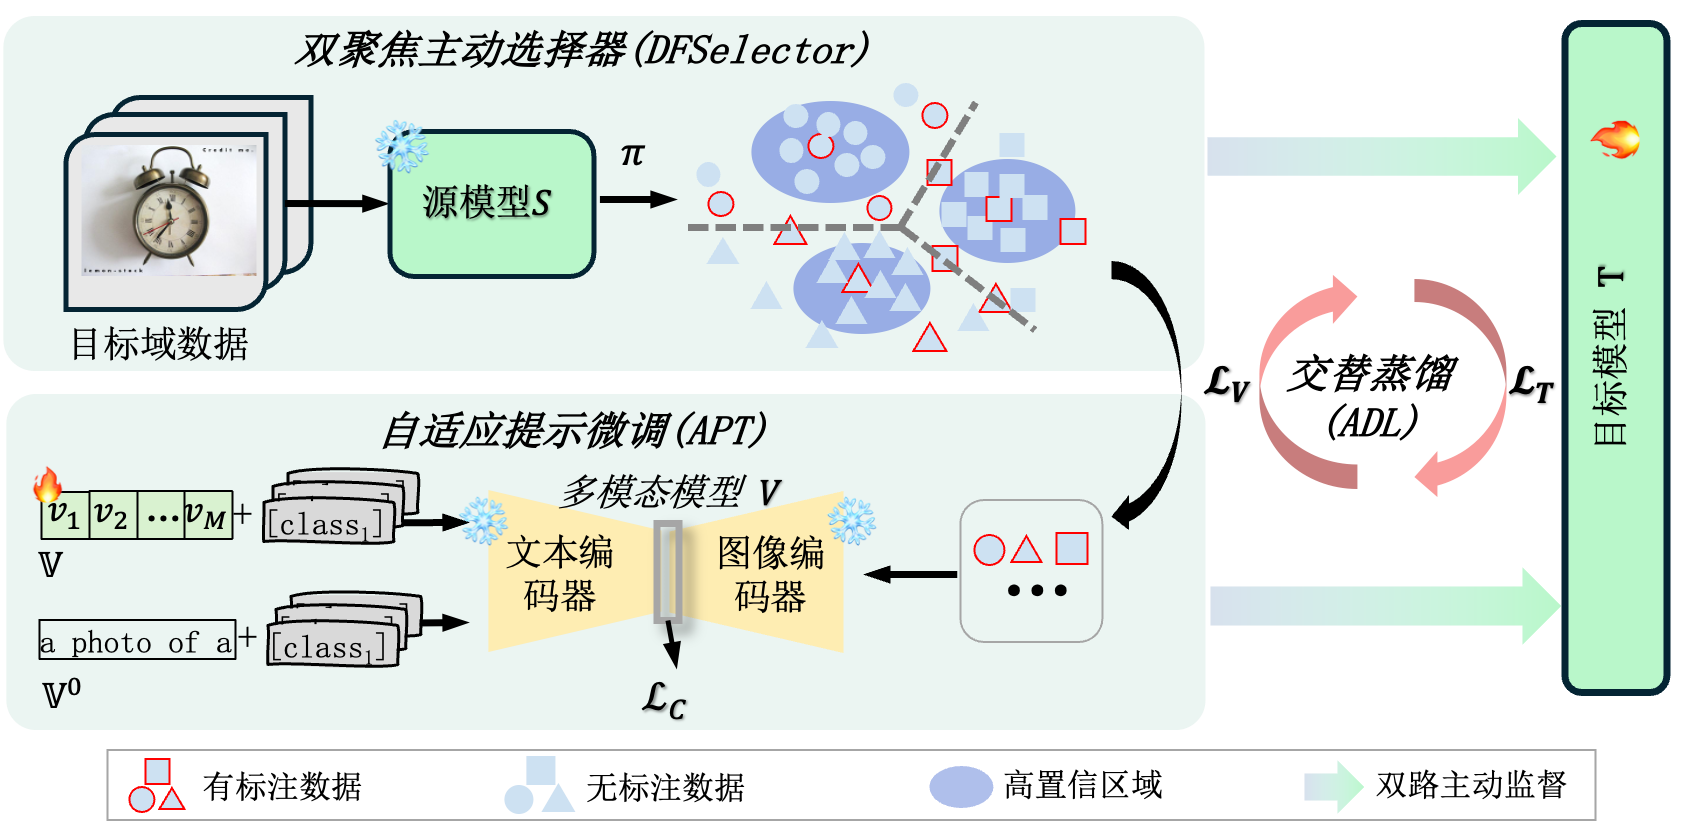
\includegraphics[width=0.9\textwidth]{chap4/damf_framework.png}
    \bicaption[fig:damf_framework]{}{DAMF总体框架示意图}{Fig.}{Overview of DAMF framework}
\end{figure}

\begin{enumerate}
    \item DFSelector对应上界中的覆盖项：协同风险上界的空间覆盖项要求所选标注集同时在 $\mathcal{X}$ 空间（源模型特征空间）与 $\mathcal{Z}$ 空间（ViL 特征空间）下提供充分的样本代表性。
    % 然而两者表征结构存在本质差异：源模型在带标签源域上预训练，其特征呈类内紧凑、类间分离的聚类结构，决策边界附近的样本最富含信息量；而 ViL 模型在零样本设定下未见过源域数据，存在显著域偏置，需要域不变的高置信锚点与 ViL 文本嵌入对齐。基于此观察，DFSelector 分别采用 MH Points 策略（针对 $\mathcal{X}$ 空间筛选边界样本，压减 $d_X(x',\mathcal{T}_q)$）与 Core-Set 策略（针对 $\mathcal{Z}$ 空间保障几何覆盖，压减 $d_Z(\phi(x'),\mathcal{T}_q)$），通过加权组合 $\mathcal{T}_q = \alpha\mathcal{T}_{\text{CO}} + (1-\alpha)\mathcal{T}_{\text{MH}}$ 构造最终标注集，统一服务两空间的覆盖需求。
    \item APT对应上界中的经验风险项与 $\eta_{\mathcal{G}}$ 的 ViL 误差子项：上界的经验风险项 $L_{\tilde{Q}}(f_P,f'_P)$ 要求 ViL 标注函数在标注集上贴近真实标注函数，$\eta_{\mathcal{G}}$ 中的 $L(g_V(x),f'_P(x))$ 要求 ViL 模型自身在目标域上的标注误差足够小，二者共同要求在有限主动标注下激活 ViL 模型的任务感知能力。
    % 全参数微调容易过拟合到有限的标注样本上，导致 ViL 模型丧失原有的跨模态泛化能力。APT 采用有监督 prompt learning 策略，仅优化 ViL 模型的类别 prompt $\{V_k\}_{k=1}^{C}$，保持图像与文本编码器冻结；其交叉熵项即为 $L(f_P,f'_P)$ 在 $\mathcal{T}_q$ 上的经验估计，同时通过知识保持正则 $\mathcal{L}_{\text{kg}}$ 将适配后的文本嵌入 $\mathbf{w}_k$ 锚定到原始泛化嵌入 $w_k^0$ 附近，避免灾难性遗忘。APT 阶段既为后续蒸馏提供了初步对齐的 ViL 教师，也在闭集与开放集两种设定下共用同一目标。
    \item ADL对应上界中 $\eta_{\mathcal{G}}$ 的跨模型对齐子项：上界要求目标模型与 ViL 模型在所有无标签目标数据上的预测一致，即压减 $L(h(x),g_V(x))$。ADL 设计双向不对称蒸馏机制实现目标模型与ViL模型之间的知识互补。
    % ：$\theta_t\!\leftarrow\!\theta_v$ 路径采用 ViL 模型的硬伪标签（$\tau_V\to0$），在形式上即为对 $L(h(x),g_V(x))$ 的直接最小化，为 $\theta_t$ 提供清晰的判别指引；$\theta_v\!\leftarrow\!\theta_t$ 路径采用 $\theta_t$ 的软标签（$\tau_T=\tau_V=1$），向 ViL 模型传递类别间关系信息，同时继续压减 $L(g_V(x),f'_P(x))$。
    % 两条路径通过统一师生概率分布（带权重的样本再加权）、统一选择掩码（闭集 / 开放集兼容的样本筛选）实现协同，配合熵最小化与多样性正则保证蒸馏过程的稳定性与类别平衡。
\end{enumerate}


训练结束后，ViL 模型被丢弃，仅使用目标模型 $\theta_t$ 进行闭集推理；在开放集推理时，则联合使用 $\theta_t$ 和 $\theta_v$ 进行未知类别检测。

\subsection{基于多模态引导的主动域适应}

\noindent\textbf{双聚焦主动样本选择器DFSelector}

由定理 3.1，协同SFADA需要同时在$\mathcal{X}$空间（源模型特征空间）和$\mathcal{Z}$空间（ViL特征空间）下优化样本覆盖项。然而，两个模型的表征结构存在本质差异：源模型在带标签源域数据上预训练，其特征空间呈现类内紧凑、类间分离的聚类结构；而ViL模型在零样本设定下未见过源域数据，其表征与目标域之间存在显著域偏置~\cite{ge2023domain,tang2024source}。因此，统一的样本选择策略难以同时满足两个假设空间的需求。本节提出双聚焦主动样本选择器 DFSelector，分别为两个假设空间设计专属选择策略，并通过加权组合形成最终的标注集。首先介绍两种选择策略：

(1)源模型假设空间下的MH点集

MH 点集~\cite{wang2023mhpl}通过邻居环境不确定性度量样本的边界性，其核心思想与引理3.2的优化目标高度契合。给定目标样本$x$，其邻居环境不确定性定义为$\mathrm{NEU}(x)=\mathrm{NP}(x)\cdot\mathrm{NA}(x)$，其中，在$x$的$q$近邻集合$\{N_1,\cdots,N_q\}$中统计各类别占比$p_1,\cdots,p_{C_t}$，则$\mathrm{NP}(x)=-\sum_{k=1}^{C_t}p_k\log p_k$，刻画邻居标签的一致程度；$\mathrm{NA}(x)=\frac{1}{q}\sum_{i=1}^{q}s_{|N_i}$，其中$s_{|N_i}$表示$x$与其近邻的特征相似度，衡量邻居的几何紧凑程度。

MH 点集从两方面契合引理 3.2 的目标风险优化目标：

\begin{itemize}
    \item 覆盖性。 对按邻居扰动排序后的候选样本，仅当其邻居集合中无已纳入样本时才将其加入标注集，由此在 $\mathcal{T}$ 上形成局部覆盖，避免冗余样本聚集。
    \item 近界性。 损失函数 $L$ 的正则性假设对回归损失（如 $\ell_p$ 范数）成立，但对有界且不随距离线性增长的分类损失（如交叉熵）通常不再成立；DBALDA~\cite{mathelin2022discrepancy} 已证明，决策边界附近的样本比远离边界的样本更具信息量。MH Points 通过 NP 与 NA 指标筛取决策边界附近样本，最大化单标注样本的信息增益。
\end{itemize}


(2) ViL模型假设空间下的Core-Set

ViL模型受域偏置和零样本误差影响，难以准确捕获目标域的类别结构~\cite{ge2023domain,tang2024source}。为优化$\mathcal{Z}$空间下的覆盖项，本章借鉴DBALDA理论~\cite{mathelin2022discrepancy}的分析：在源域与目标域标注函数一致（$f=f_P=f_Q$）、$f\in\mathcal{H}$ 且 $\epsilon=0$ 的简化条件下，引理 3.1 与引理 3.2 的目标风险上界仍可重写为以覆盖项为主导的形式，因此可以采用与域适应无关的纯主动学习方法。在此理论支撑下，本章选择Core-Set~\cite{prabhu2021active}作为$\mathcal{Z}$空间下的采样策略，其选择过程可形式化为 $k$-中心问题：在 $\mathcal{T}$ 上选取 $k$ 个样本，使 $\mathcal{Z}$ 空间内未选样本到最近已选样本的最大距离最小化，即最小化最大覆盖半径 $\max_{x'\in\mathcal{T}}d_Z(x',\mathcal{T}_{\text{CO}})$。
具体而言，对每个类别$k$，选取源模型预测置信度最高的样本作为该类别的代表：
\begin{equation}
\mathcal{T}_{\text{CO}} = \{\arg\max_{x\in\mathcal{T}}\theta_s^{(k)}(x) : k\in\mathcal{C}\}.
\end{equation}

这种构造方式具有双重优势：（1）高源模型置信度样本具备类别判别性且具有域不变的类别锚点特性，可与ViL文本嵌入自然对齐，避免直接多模态匹配引入的偏差；（2）所选样本在ViL特征空间中形成紧凑簇结构，可近似$k$-中心问题的解，最大化$\mathcal{Z}$空间的覆盖。


为联合优化双假设空间下的覆盖项，最终的标注集$\mathcal{T}_q$通过加权组合构建：
\begin{equation}
\mathcal{T}_q = \alpha \cdot \mathcal{T}_{\text{CO}} + (1-\alpha)\cdot\mathcal{T}_{\text{MH}},
\label{eq:dfselector}
\end{equation}
其中$\alpha\in[0,1]$控制两类样本的比例。当$\alpha$较大时，标注集偏向$\mathcal{Z}$空间的几何覆盖；当$\alpha$较小时，偏向$\mathcal{X}$空间的边界信息捕获。实验表明，$\alpha=0.4$时在Office-Home数据集上达到最优平衡。

\noindent\textbf{多模态自适应提示微调APT}

DFSelector获得的标注集$\mathcal{T}_q$为ViL模型的域适配提供了宝贵的监督信号。由于主动采样比例$\rho$较小，直接对ViL模型进行全参数微调容易过拟合到有限的标注样本上，导致其丧失原有的开放词汇泛化能力。本节采用有监督prompt learning策略~\cite{zhou2022learning}，仅优化ViL模型的类别prompt $\{V_k\}_{k=1}^{C}$，而保持图像编码器和文本编码器参数冻结。该设计的选择基于以下两点考虑：（1）prompt tuning 已被证明是 CLIP 类模型参数高效适配的有效手段；（2）ViL模型的核心优势源于其多模态对齐所蕴含的强泛化能力，应在适配过程中予以保留。

具体地，APT通过最小化如下损失函数优化prompt：
\begin{equation}
\mathcal{L}_C = \mathcal{L}_{\text{CE}} + \lambda \mathcal{L}_{\text{kg}} = \mathbb{E}_{x\in\mathcal{T}_q}\mathrm{CE}\big(e_y \| p_V(x)\big) + \frac{\lambda}{C_t}\sum_{k=1}^{C_t}\|w_k - w_k^0\|_2^2,
\label{eq:apt_loss}
\end{equation}
其中$e_y$为真实标签$y$的独热向量，$\mathcal{L}_{\text{kg}}$为知识保持正则项，$\mathbf{w}_k^0=\mathrm{Enc}_t(V_k^0)$为原始prompt模板“a photo of a [$c_k$]”生成的文本嵌入。$\mathcal{L}_{\text{kg}}$通过将适配后的文本嵌入$w_k$锚定到原始泛化嵌入$w_k^0$附近，防止ViL模型在少量标注上过拟合而丧失基础泛化能力。超参数$\lambda$控制正则强度。

\noindent\textbf{多协作模型交替蒸馏学习ADL}

APT阶段仅在主动标注样本上对ViL模型进行了初步适配，尚未充分挖掘ViL模型对全部无标签目标数据的零样本预测价值。为此，本节设计交替蒸馏 ADL 机制，通过双向不对称蒸馏实现目标模型$\theta_t$与ViL模型$\theta_v$之间的知识互补。该机制的设计灵感来自定理 3.4 中揭示的第三项优化目标跨模型对齐损失$L(h(x),g_V(x))$。

为统一两类模型的输出形式，本章将目标模型与ViL模型抽象为学生$A\in\{\theta_t,\theta_v\}$与教师$B\in\{\theta_v,\theta_t\}$的组合。在蒸馏过程中，已标注样本$\mathcal{T}_q$使用真实标签作为教师信号，未标注样本$\mathcal{T}\setminus\mathcal{T}_q$使用教师模型的预测作为伪监督。同时，借鉴自训练方法~\cite{liang2021source}的样本加权策略，对不同来源的样本施加不同的权重以强调可靠监督：
\begin{equation}
\big(\tilde{p}_{A\leftarrow B}(x), W(x)\big) =
\begin{cases}
(e_y, \beta_q), & x\in\mathcal{T}_q, y\text{为真实标签};\\
\big(\Pi_{A\leftarrow B}(\mathrm{softmax}(\theta_B(x)/\tau_B)), \beta\big), & x\in\mathcal{T}\setminus\mathcal{T}_q.
\end{cases}
\label{eq:teacher_dist}
\end{equation}
其中$\beta_q\geq\beta>0$为样本权重超参数，$\Pi_{A\leftarrow B}$为可选的概率映射函数。学生模型的预测为$p_A^{\tau_A}(x)=\mathrm{softmax}(\theta_A(x)/\tau_A)$。值得注意的是，当$\tau_B\to 0$时，教师分布退化为独热硬标签。

为缓解蒸馏过程中的伪标签噪声，本章引入二元掩码$m_{A\leftarrow B}(x)\in\{0,1\}$控制参与蒸馏的样本集合。掩码设计同时兼容闭集与开放集两种设定：
\begin{align}
m_{V\leftarrow T}(x) &= \mathbf{1}\{x\in\mathcal{X}_{\text{top}}\cup\mathcal{T}_q\}, &\\
m_{T\leftarrow V}(x) &= \mathbf{1}\{x\in\hat{\mathcal{T}}_t\cup\mathcal{T}_q\}, &\\[3pt]
\mathcal{X}_{\text{top}} &= \bigcup_{y\in\mathcal{Y}_t}\mathrm{top}\text{-}N\big\{\max_k p_T^{(k)}(x) : \hat{y}_T(x)=y\big\}, \label{eq:topX} &\\[3pt]
\hat{\mathcal{T}}_t &=
\begin{cases}
\mathcal{T}, & \mathcal{Y}_s=\mathcal{Y}_t;\\
\{x\in\mathcal{T}: \arg\max_k\tilde{p}_{T\leftarrow V}^{(k)}(x)\in\mathcal{Y}_s\}, & \mathcal{Y}_s\subset\mathcal{Y}_t.
\end{cases}
\end{align}
其中$\mathcal{X}_{\text{top}}$为目标模型每个类别内预测置信度最高的$N$个样本集合，$\hat{\mathcal{T}}_t$在开放集设定下进一步筛选出ViL模型预测属于已知类别的样本，避免未知类别样本污染蒸馏过程。

基于上述定义，两条蒸馏路径的损失函数分别为：

$\theta_t\leftarrow\theta_v$蒸馏： ViL模型采用余弦相似度作为输出，其预测分布相对平坦。为给目标模型提供清晰的监督信号，采用硬标签蒸馏策略：
\begin{equation}
\mathcal{L}_{T\leftarrow V}^{dist} = -\mathbb{E}_{x\in\mathcal{T}}m_{T\leftarrow V}(x)W(x)\mathrm{CE}\big(\tilde{p}_{T\leftarrow V}(x) \| p_T^{\tau_T}(x)\big),
\label{eq:dist_t_from_v}
\end{equation}
其中$\tau_T=1$，$\tau_V\to 0$，使教师分布退化为硬伪标签。

$\theta_v\leftarrow\theta_t$蒸馏： 目标模型的分类输出更具判别性，使用软标签蒸馏可传递更丰富的类别间关系信息：
\begin{equation}
\mathcal{L}_{V\leftarrow T}^{dist} = -\mathbb{E}_{x\in\mathcal{T}}m_{V\leftarrow T}(x)W(x)\mathrm{CE}\big(\tilde{p}_{V\leftarrow T}(x) \| p_V^{\tau_V}(x)\big),
\label{eq:dist_v_from_t}
\end{equation}
其中$\tau_T=\tau_V=1$，并使用恒等映射$\Pi_{V\leftarrow T}$实现标准知识蒸馏。

借鉴信息最大化（IM）损失~\cite{gomes2010discriminative}的设计，本章在目标模型上额外引入熵最小化和多样性正则化损失，使跨信号源的互补信息在学习层面转化为目标模型的判别能力：
\begin{align}
\mathcal{L}_{\text{ent}} & = \mathbb{E}_{x\in\mathcal{T}}m_{T\leftarrow V}(x)\mathrm{CE}\big(p_T(x) \| p_T(x)\big), 
\label{eq:loss_ent}\\
\mathcal{L}_{\text{div}} & = \sum_{k=1}^{C}\hat{p}_k\log\hat{p}_k = \mathrm{KL}\big(\hat{p},\tfrac{1}{C}\mathbf{1}_C\big) - \log C, 
\label{eq:loss_div}
\end{align}
其中$\hat{p}=\mathbb{E}_{x\in\hat{\mathcal{T}}_t}[p_T(x)]$为全体目标样本的平均输出。$\mathcal{L}_{\text{ent}}$鼓励模型对未标注样本产生确定性预测，$\mathcal{L}_{\text{div}}$防止模型将预测集中于少数类别。

最终，目标模型与ViL模型的训练损失分别为：
\begin{align}
\mathcal{L}_T &= \mathcal{L}_{T\leftarrow V}^{dist} + \mathcal{L}_{\text{ent}} + \mathcal{L}_{\text{div}},
\label{eq:loss_T}\\
\mathcal{L}_V &= \mathcal{L}_{V\leftarrow T}^{dist} + \lambda \mathcal{L}_{\text{kg}}.
\label{eq:loss_V}
\end{align}

推理阶段，闭集场景下仅使用目标模型：$O=\arg\max_{k\in\mathcal{Y}_t}\theta_t^{(k)}(x)$；开放集场景下，首先利用ViL模型识别未知类别，若$\arg\max_{k\in\mathcal{Y}_t}\theta_v^{(k)}(x)\in\mathcal{Y}_t\setminus\mathcal{Y}_s$则判定为未知样本，否则使用目标模型的预测结果。


\begin{algorithm}[!htb]
    \AlgoBiCaption{DAMF 算法训练流程}{Training procedure of DAMF}
    \label{alg:damf}
    \small
    \KwIn{源模型$\theta_s$；无标签目标域$\mathcal{T}$；标注预算$\rho$；ViL模型$\theta_v$；超参数$\alpha,\beta,\beta_q,\lambda,N$}
    \KwOut{适应后的目标模型$\theta_t$与ViL模型$\theta_v$}
    \BlankLine
    \tcp{阶段1：双聚焦主动样本选择}
    根据式\eqref{eq:dfselector}构建标注集$\mathcal{T}_q = \alpha\mathcal{T}_{\text{CO}} + (1-\alpha)\mathcal{T}_{\text{MH}}$，并由专家标注;\\
    \BlankLine
    \tcp{阶段2：自适应提示微调}
    \For{epoch $= 1$ \textbf{to} $E_{APT}$}{
        从$\mathcal{T}_q$采样小批量样本;\\
        根据式\eqref{eq:apt_loss}更新ViL prompt：$V \leftarrow V - \eta_V\nabla\mathcal{L}_C$;\\
    }
    \BlankLine
    \tcp{阶段3：交替蒸馏}
    初始化$\theta_t\leftarrow\theta_s$;\\
    \For{epoch $= 1$ \textbf{to} $E_{ADL}$}{
        根据式\eqref{eq:teacher_dist}构建教师分布$\tilde{p}_{A\leftarrow B}$;\\
        计算$\mathcal{X}_{\text{top}}$与$\hat{\mathcal{T}}_t$，构建掩码$m_{A\leftarrow B}$;\\
        \For{iter}{
            根据式\eqref{eq:loss_T}计算$\mathcal{L}_T$;
            根据式\eqref{eq:loss_V}计算$\mathcal{L}_V$;\\
            更新$\theta_t$与$V$：$\theta_t\leftarrow\theta_t - \eta_T\nabla\mathcal{L}_T$，$V\leftarrow V - \eta_V\nabla\mathcal{L}_V$;
        }
    }
    \Return $\theta_t$, $\theta_v$
\end{algorithm}

\section{实验结果和分析}

\subsection{数据集与实验设置}

本章在四个广泛使用的SFADA基准数据集上评估方法的有效性，包括小规模 Office 数据集~\cite{saenko2010adapting}（Amazon、Dslr、Webcam 三个领域，分别标记为 A、D、W，共 31 类）、中等规模 Office-Home 数据集~\cite{venkateswara2017deep}（Art、Clipart、Product、Real-World 四个领域，分别标记为 A、C、P、R，共 65 类）、大规模合成到真实（Synthetic $\rightarrow$ Real, SR）适应任务 VisDA-C~\cite{peng2017visda}（12 类），以及 DomainNet 的 126 类子集 miniDomainNet（Clipart、Painting、Real、Sketch 四个领域，分别标记为 C、P、R、S，构成 12 个跨域任务）。

开放集设置参考已有工作~\cite{liu2021separate}的设定：Office数据集按字母序前10个类别为已知、后11个为未知；Office-Home前25个类别为已知、后40个为未知；VisDA-C前6个类别为已知、后6个为未知。
闭集场景下报告所有目标样本的平均分类准确率；开放集场景下报告HOS（Harmonic Open-set Score）分数，定义为已知类别准确率$\mathrm{acc}_{kn}$与未知类别准确率$\mathrm{acc}_{ukn}$的调和平均值：$\mathrm{HOS}=2\cdot\mathrm{acc}_{kn}\cdot\mathrm{acc}_{ukn}/(\mathrm{acc}_{kn}+\mathrm{acc}_{ukn})$。

源域预训练采用与SHOT~\cite{liang2021source}相同的流程：在Office/Office-Home/miniDomainNet上使用ResNet-50~\cite{he2016deep}，在VisDA-C上使用ResNet-101。ViL模型默认采用CLIP ViT-B/32图像编码器。DFSelector中$\alpha=0.4$，$\mathcal{X}_{\text{top}}$大小$N=16$，$\beta_q=3$，$\beta=0.3$，闭集设定$\lambda=1$，开放集设定$\lambda=8$。APT阶段使用SGD优化器，基础学习率$2\times 10^{-3}$，热启动的首个epoch学习率$1\times 10^{-5}$ 后接$E_{APT}=50$个epoch的余弦退火。ADL阶段目标模型学习率$1\times 10^{-2}$，ViL prompt学习率$2\times 10^{-3}$，共训练$E_{ADL}=20$个epoch。所有实验在单张NVIDIA RTX 4090 GPU上运行，默认标注预算$\rho=5\%$。


本节在闭集与开放集两种域适应设定下与现有方法进行系统对比。

闭集设定下的对比方法涵盖以下五类：（1）仅源域模型（Source-only）与基于ViT-B/32骨干的零样本CLIP方法（Zero-Shot CLIP with ViT-B/32 backbone, ZS-C-B32）；（2）无监督域适应（Unsupervised Domain Adaptation, UDA）方法；（3）无源域适应（Source-Free Domain Adaptation, SFDA）方法；（4）主动域适应（Active Domain Adaptation, ADA）方法；（5）无源主动域适应（Source-Free Active Domain Adaptation, SFADA）方法。为保证对比公平，本章基于官方代码复现DIFO-C-B32（与本文采用相同的源模型），并通过引入MH点（MHPL~\cite{wang2023mhpl}中的多假设样本）将其扩展至SFADA设定，记为MHPL+DIFO-C-B32。

开放集设定下的对比方法包括以下四类：（1）仅源域模型与ZS-C-B32；（2）开放集无源域适应（Open-Set Source-Free Domain Adaptation, OSSFDA）方法；（3）开放集域适应（Open-Set Domain Adaptation, OSDA）方法；（4）开放集无源主动域适应（Open-Set Source-Free Active Domain Adaptation, OSSFADA）方法。其中，MHPL被扩展为开放集版本MHPL-O：采用2类k-means聚类将目标样本划分为已知与未知两簇，将高熵簇识别为未知类别，并将主动采样限制在已知类别簇内进行。

\subsection{实验结果对比}

表~\ref{tab:closed_oh_visda}给出了在Office-Home与VisDA-C数据集上的闭集实验结果。DAMF在所有任务上均显著优于现有SFADA方法，相较于最优基线BIAS~\cite{wang2024bias}在Office-Home上提升4.5\%，在VisDA-C上提升1.5\%。尤为重要的是，DAMF甚至超越了依赖源域数据访问的UDA和ADA方法，验证了多模态融合在低资源SFADA场景下的独特价值。

\begin{table}[!htbp]
    \bicaption[tab:closed_oh_visda]{}{闭集域适应在Office-Home与VisDA-C数据集上的准确率对比}{Table}{Closed-set accuracy on Office-Home and VisDA-C under 5\% budget}
    \vspace{0.5em}\centering\wuhao
    \setlength{\tabcolsep}{1pt}
    \resizebox{\textwidth}{!}{
    \begin{tabular}{llccccccccccccccc}
    \toprule
    类别 & 方法 & ViL & \multicolumn{13}{c}{Office-Home} & VisDA-C \\
    \cline{4-16}\cline{17-17}
    &&& AC & AP & AR & CA & CP & CR & PA & PC & PR & RA & RC & RP & Avg & SR \\
    \midrule
    Zero-shot & Source-only & $\times$ & 43.4 & 65.2 & 71.8 & 52.2 & 60.2 & 63.0 & 52.2 & 39.6 & 72.5 & 64.4 & 43.4 & 76.5 & 58.7 & 46.9 \\
    & ZS-C-B32~\cite{radford2021learning} & $\checkmark$ & 58.3 & 79.7 & 78.6 & 71.9 & 79.7 & 78.6 & 71.9 & 58.3 & 78.6 & 71.9 & 58.3 & 79.7 & 72.2 & 87.2 \\
    \midrule
    UDA & DAPL~\cite{ge2023domain} & $\checkmark$ & 54.1 & 84.3 & 84.8 & 74.4 & 83.7 & 85.0 & 74.5 & 54.6 & 84.8 & 75.2 & 54.7 & 83.8 & 74.5 & 86.9 \\
    & PADCLIP-RN~\cite{lai2023padclip} & $\checkmark$ & 57.5 & 84.0 & 83.8 & 77.8 & 85.5 & 84.7 & 76.3 & 59.2 & 85.4 & 78.1 & 60.2 & 86.7 & 76.6 & 88.5 \\
    \midrule
    SFDA & SHOT~\cite{liang2021source} & $\times$ & 57.1 & 78.1 & 81.5 & 68.0 & 78.2 & 78.1 & 67.4 & 54.9 & 82.2 & 73.3 & 58.8 & 84.3 & 71.8 & 82.4 \\
    & A2Net~\cite{xia2021adaptive} & $\times$ & 58.4 & 79.0 & 82.4 & 67.5 & 79.3 & 78.9 & 68.0 & 56.2 & 82.9 & 74.1 & 60.5 & 85.0 & 72.8 & 84.3 \\
    & DIFO-C-B32~\cite{tang2024source} & $\checkmark$ & 63.4 & 83.1 & 82.0 & 74.2 & 83.5 & 82.6 & 74.5 & 64.4 & 83.8 & 75.2 & 65.0 & 84.1 & 76.3 & 90.1 \\
    \midrule
    ADA & CLUE~\cite{prabhu2021active} & $\times$ & 58.0 & 79.3 & 80.9 & 68.8 & 77.5 & 76.7 & 66.3 & 57.9 & 81.4 & 75.6 & 60.8 & 86.3 & 72.5 & -- \\
    & EADA~\cite{xie2022active} & $\times$ & 63.6 & 84.4 & 83.5 & 70.7 & 83.7 & 80.5 & 73.0 & 63.5 & 85.2 & 79.4 & 65.4 & 88.6 & 76.7 & 88.3 \\
    & CA-ADA~\cite{xiao2024category} & $\times$ & 69.2 & 88.4 & 86.3 & 68.9 & 84.5 & 82.7 & 69.8 & 67.9 & 88.3 & 79.6 & 92.1 & 74.2 & 79.3 & -- \\
    \midrule
    SFADA & CoreSet~\cite{prabhu2021active} & $\times$ & 61.8 & 81.8 & 83.3 & 71.1 & 82.9 & 81.6 & 70.7 & 60.5 & 84.7 & 76.1 & 61.7 & 86.1 & 75.2 & 85.9 \\
    & Entropy~\cite{wang2014new} & $\times$ & 65.0 & 84.0 & 85.9 & 71.8 & 83.8 & 82.6 & 70.7 & 63.8 & 85.1 & 77.8 & 64.1 & 88.1 & 76.9 & 86.7 \\
    & ELPT~\cite{li2022source} & $\times$ & 65.3 & 84.1 & 84.9 & 72.9 & 84.4 & 82.8 & 69.8 & 63.3 & 86.1 & 76.2 & 65.6 & 89.1 & 77.0 & 89.2 \\
    & MHPL+DIFO-C-B32 & $\checkmark$ & 65.0 & 83.7 & 83.1 & 75.0 & 84.3 & 83.6 & 75.4 & 66.3 & 84.5 & 76.4 & 66.2 & 84.6 & 77.4 & 90.5 \\
    & SQAdapt~\cite{li2023source} & $\times$ & 65.2 & 85.4 & 85.9 & 72.1 & 84.4 & 84.2 & 72.2 & 64.8 & 85.9 & 77.5 & 65.6 & 89.9 & 77.8 & -- \\
    & MHPL~\cite{wang2023mhpl} & $\times$ & 69.0 & 85.7 & 86.4 & 72.6 & 87.4 & 84.2 & 73.3 & 67.4 & 86.4 & 80.1 & 69.6 & 89.8 & 79.3 & 91.3 \\
    & MHPL+BIAS~\cite{wang2024bias} & $\times$ & 70.3 & 88.0 & 86.9 & 74.1 & 88.5 & 84.9 & 73.1 & 69.1 & 87.2 & 80.4 & 70.7 & 90.7 & 80.3 & 91.1 \\
    % \midrule
    &\textbf{DAMF}  & $\checkmark$ & \textbf{76.3} & \textbf{91.7} & \textbf{90.2} & \textbf{79.6} & \textbf{92.5} & \textbf{90.1} & \textbf{79.9} & \textbf{76.1} & \textbf{90.1} & \textbf{81.2} & \textbf{76.5} & \textbf{93.1} & \textbf{84.8} & \textbf{92.6} \\
    \bottomrule
    \end{tabular}
    }
\end{table}

表~\ref{tab:closed_minidn} 给出了miniDomainNet数据集上的结果。DAMF在12个跨域任务上均取得最优性能，平均准确率达86.6\%，相较于先前的CLIP基SFDA方法MHPL+DIFO-C-B32提升5.5\%。这一显著的领先优势表明，miniDomainNet类别数较多（126类），类别判别难度更大，此时ViL模型的语义先验知识对目标模型的辅助价值更加突出。

\begin{table}[!htbp]
    \bicaption[tab:closed_minidn]{}{闭集域适应在miniDomainNet数据集上的准确率（\%）对比（标注预算5\%）}{Table}{Closed-set accuracy (\%) on miniDomainNet under 5\% budget}
    \vspace{0.5em}\centering\wuhao
    \resizebox{\textwidth}{!}{
    \begin{tabular}{llcccccccccccccc}
    \toprule
    类别 & 方法 & ViL & CP & CR & CS & PC & PR & PS & RC & RP & RS & SC & SP & SR & Avg \\
    \midrule
    Zero-shot & Source-only & $\times$ & 47.5 & 61.0 & 49.6 & 56.1 & 74.9 & 50.6 & 58.3 & 63.5 & 48.9 & 59.4 & 52.9 & 61.0 & 57.0 \\
    & ZS-C-B32 & $\checkmark$ & 77.3 & 90.0 & 74.2 & 78.6 & 90.0 & 74.2 & 78.6 & 77.3 & 74.2 & 78.6 & 77.3 & 90.0 & 80.0 \\
    \midrule
    SFDA & SHOT & $\times$ & 60.3 & 78.7 & 58.5 & 63.5 & 80.3 & 60.6 & 68.1 & 66.8 & 65.6 & 66.8 & 59.5 & 75.3 & 67.0 \\
    & DIFO-C-B32 & $\checkmark$ & 76.6 & 87.7 & 75.0 & 78.6 & 87.6 & 75.4 & 79.8 & 77.0 & 75.3 & 79.2 & 76.6 & 87.6 & 79.7 \\
    \midrule
    SFADA & SQAdapt & $\times$ & 65.5 & 82.0 & 66.2 & 68.8 & 84.0 & 65.3 & 72.2 & 70.5 & 67.2 & 69.8 & 66.6 & 80.7 & 71.6 \\
    & MHPL & $\times$ & 70.4 & 86.6 & 69.3 & 76.1 & 87.8 & 70.0 & 75.0 & 71.3 & 67.1 & 77.6 & 71.1 & 86.6 & 75.7 \\
    & MHPL+DIFO-C-B32 & $\checkmark$ & 78.0 & 89.0 & 76.3 & 79.8 & 89.1 & 76.8 & 81.0 & 78.8 & 76.8 & 80.3 & 78.2 & 88.9 & 81.1 \\
    % \midrule
    &\textbf{DAMF}  & $\checkmark$ & \textbf{84.7} & \textbf{92.9} & \textbf{81.7} & \textbf{86.8} & \textbf{93.5} & \textbf{82.1} & \textbf{86.7} & \textbf{85.2} & \textbf{81.7} & \textbf{86.5} & \textbf{84.8} & \textbf{93.1} & \textbf{86.6} \\
    \bottomrule
    \end{tabular}
    }
\end{table}

表~\ref{tab:closed_office}给出了Office数据集的结果。在小规模数据集上DAMF同样取得了94.2\%的平均准确率，相较于MHPL+BIAS提升0.6\%。综合三个数据集的结果可知，DAMF在各种数据规模和域差异条件下均展现出一致的优越性。

\begin{table}[!htbp]
    \centering
    \begin{minipage}[t]{0.48\textwidth}
        \centering
        \wuhao
        \bicaption[tab:closed_office]{}{闭集域适应在Office数据集上的准确率对比}{Table}{Closed-set accuracy on Office under 5\% budget}
        \vspace{0.5em}
        \resizebox{\linewidth}{!}{
        \begin{tabular}{lccccccc}
        \toprule
        方法 & AD & AW & DA & DW & WA & WD & Avg \\
        \midrule
        Source-only & 79.3 & 72.6 & 60.0 & 93.7 & 61.6 & 96.0 & 77.2 \\
        ZS-C-B32 & 81.7 & 79.8 & 77.1 & 79.8 & 77.1 & 81.7 & 79.5 \\
        \midrule
        SHOT & 94.0 & 90.1 & 74.7 & 98.4 & 74.3 & 99.9 & 88.6 \\
        A2Net & 94.5 & 94.0 & 76.7 & 99.2 & 76.1 & 100.0 & 90.1 \\
        DIFO-C-B32 & 96.2 & 95.2 & 83.5 & 98.0 & 83.9 & 98.8 & 92.6 \\
        \midrule
        CLUE & 92.0 & 87.3 & 79.0 & 99.2 & 79.6 & 99.8 & 89.5 \\
        EADA & 97.7 & 96.6 & 82.1 & 100.0 & 82.8 & 100.0 & 93.2 \\
        \midrule
        CoreSet & 93.4 & 92.5 & 78.4 & 99.1 & 78.2 & 100.0 & 90.3 \\
        Entropy & 95.6 & 95.4 & 80.3 & 99.1 & 80.1 & 100.0 & 91.8 \\
        ELPT & 98.0 & 97.2 & 81.2 & 99.4 & 80.7 & 100.0 & 92.8 \\
        MHPL & 97.8 & 96.7 & 82.5 & 99.3 & 82.6 & 100.0 & 93.2 \\
        MHPL+BIAS & 97.8 & 97.1 & 83.1 & 99.1 & 84.4 & 100.0 & 93.6 \\
        \textbf{DAMF} & \textbf{97.6} & \textbf{97.6} & \textbf{85.6} & \textbf{98.4} & \textbf{86.6} & \textbf{99.2} & \textbf{94.2} \\
        \bottomrule
        \end{tabular}}
    \end{minipage}
    \hfill
    \begin{minipage}[t]{0.48\textwidth}
        \centering
        \wuhao
        \bicaption[tab:openset_office]{}{开放集域适应在Office数据集上的HOS对比}{Table}{Open-set HOS on Office under 5\% budget}
        \vspace{0.5em}
        \resizebox{\linewidth}{!}{
        \begin{tabular}{lccccccc}
        \toprule
        方法 & AD & AW & DA & DW & WA & WD & Avg \\
        \midrule
        Source-only & 70.1 & 68.8 & 70.3 & 88.1 & 63.3 & 92.9 & 75.6 \\
        ZS-C-B32 & 92.4 & 90.0 & 91.8 & 90.0 & 91.8 & 92.4 & 91.4 \\
        \midrule
        SHOT-O & 80.2 & 71.6 & 64.3 & 93.1 & 64.0 & 91.8 & 77.5 \\
        GLC~\cite{qu2023up} & 82.6 & 74.6 & 92.6 & 96.0 & 91.8 & 96.1 & 89.0 \\
        LEAD~\cite{qu2024lead} & 84.9 & 85.1 & 90.2 & 94.8 & 90.3 & 96.5 & 90.3 \\
        \midrule
        Anna~\cite{li2023adjustment} & 83.8 & 85.5 & 82.5 & 99.5 & 81.6 & 98.4 & 88.6 \\
        PRIS~\cite{tong2025reserve} & 92.9 & 93.0 & 90.9 & 99.0 & 90.7 & 98.8 & 94.2 \\
        VLFE~\cite{liu2025open} & 93.3 & 93.4 & 91.4 & -- & 91.2 & -- & -- \\
        \midrule
        MHPL-O & 73.1 & 73.9 & 81.0 & 94.9 & 77.0 & 92.4 & 82.1 \\
        DSL~\cite{wang2025active} & 88.8 & 92.5 & 85.2 & 97.8 & 87.0 & 92.9 & 90.7 \\
        \textbf{DAMF} & \textbf{96.3} & \textbf{94.4} & \textbf{91.7} & \textbf{97.0} & \textbf{92.4} & \textbf{99.1} & \textbf{95.2} \\
        \bottomrule
        \end{tabular}}
    \end{minipage}
\end{table}



表~\ref{tab:openset_office}和表~\ref{tab:openset_oh_visda}给出了开放集SFADA场景下的实验结果。ZS-C-B32在Office-Home/VisDA-C/Office上分别取得79.9\%/90.5\%/91.4\%的HOS分数，验证了ViL模型在开放集场景下的天然优势。而MHPL-O等方法在开放集下性能显著退化，说明现有SFADA方法在开放集场景下适应性不足。DAMF通过联合使用目标模型与ViL模型进行开放集推理，在Office-Home上较VLFE~\cite{liu2025open}提升9.7\%，较DIFO-C-B32提升11.8\%，充分证明了DAMF在开放集设定下的优越性。

\begin{table}[!htbp]
    \bicaption[tab:openset_oh_visda]{}{开放集域适应在Office-Home与VisDA-C上的HOS对比}{Table}{Open-set HOS on Office-Home and VisDA-C}
    \vspace{0.5em}\centering\wuhao
    \resizebox{\textwidth}{!}{
    \begin{tabular}{llccccccccccccccc}
    \toprule
    类别 & 方法 & ViL & \multicolumn{13}{c}{Office-Home} & VisDA-C \\
    \cline{4-16}
    &  & & AC & AP & AR & CA & CP & CR & PA & PC & PR & RA & RC & RP & Avg & SR \\
    \midrule
    Zero-shot & Source-only & $\times$ & 33.1 & 53.6 & 67.2 & 30.9 & 41.8 & 45.8 & 33.2 & 27.1 & 56.7 & 48.2 & 33.0 & 60.8 & 44.3 & 41.4 \\
    & ZS-C-B32 & $\checkmark$ & 71.9 & 85.0 & 85.3 & 77.3 & 85.0 & 85.3 & 77.3 & 71.9 & 85.3 & 77.3 & 71.9 & 85.0 & 79.9 & 90.5 \\
    \midrule
    OSSFDA & SHOT-O & $\times$ & 32.9 & 29.5 & 39.6 & 56.8 & 30.1 & 41.1 & 54.9 & 35.4 & 42.3 & 58.5 & 33.5 & 33.3 & 40.7 & 28.1 \\
    & LEAD & $\times$ & 60.7 & 70.8 & 76.5 & 61.0 & 68.6 & 70.8 & 65.5 & 59.8 & 74.2 & 64.8 & 57.7 & 75.8 & 67.2 & 74.2 \\
    & GLC & $\times$ & 65.3 & 74.2 & 79.0 & 60.4 & 71.6 & 74.7 & 63.7 & 63.2 & 75.8 & 67.1 & 64.3 & 77.8 & 69.8 & 72.5 \\
    & DIFO-C-B32 & $\checkmark$ & 64.5 & 86.2 & 87.9 & 68.2 & 79.3 & 86.1 & 67.2 & 62.1 & 88.3 & 71.9 & 65.3 & 84.4 & 75.9 & -- \\
    \midrule
    OSDA & Anna & $\times$ & 69.0 & 73.7 & 76.8 & 64.7 & 68.6 & 73.0 & 66.5 & 63.1 & 76.6 & 71.3 & 65.7 & 78.7 & 70.7 & -- \\
    & PRIS & $\times$ & 63.5 & 77.0 & 79.6 & 65.5 & 66.9 & 71.4 & 68.0 & 62.3 & 79.5 & 75.0 & 61.7 & 77.9 & 70.9 & -- \\
    & VLFE & $\checkmark$ & 71.9 & 81.9 & 83.8 & 74.1 & 82.2 & 84.0 & 74.7 & 69.7 & 84.7 & 76.6 & 70.4 & 81.8 & 78.0 & 83.4 \\
    \midrule
    OSSFADA & MHPL-O & $\times$ & 56.8 & 74.1 & 78.5 & 61.2 & 69.0 & 71.7 & 62.3 & 55.5 & 72.2 & 69.1 & 57.0 & 71.8 & 66.6 & 64.6 \\
    & DSL & $\times$ & 72.5 & 84.3 & 82.1 & 67.1 & 83.5 & 80.2 & 66.0 & 70.4 & 81.3 & 71.7 & 69.6 & 84.6 & 76.2 & 88.5 \\
    % \midrule
    &\textbf{DAMF}  & $\checkmark$ & \textbf{80.4} & \textbf{92.5} & \textbf{91.3} & \textbf{86.3} & \textbf{92.5} & \textbf{90.9} & \textbf{85.5} & \textbf{82.0} & \textbf{91.7} & \textbf{86.8} & \textbf{80.8} & \textbf{92.2} & \textbf{87.7} & \textbf{92.0} \\
    \bottomrule
    \end{tabular}}
\end{table}


\begin{figure}[!htbp]
    \centering
    \subfigure[源域模型(63.3\%)]{\includegraphics[width=0.23\linewidth]{papers/DAMF/tsne_source.pdf}
    \label{fig:res_tsne_a}
    }
\vrule
    \subfigure[ELPT(80.7\%)]{\includegraphics[width=0.23\linewidth]{papers/DAMF/tsne_ELPT.pdf}
    \label{fig:res_tsne_elpt}}
    \subfigure[MHPL(82.6\%)]{\includegraphics[width=0.23\linewidth]{papers/DAMF/tsne_MHPL.pdf}
    \label{fig:res_tsne_mhpl}}
    \subfigure[本章(86.6\%)]{\includegraphics[width=0.23\linewidth]{papers/DAMF/tsne_mine.pdf}
    \label{fig:res_tsne_mine}}
    \bicaption[fig:tsne_features]{}{不同采样策略下主动样本分布的t-SNE可视化}{Fig.}{t-SNE visualization of active samples under different strategies}
\end{figure}

图~\ref{fig:tsne_features}给出了Office数据集W$\rightarrow$A任务上目标特征在适应前后的t-SNE分布。适应前特征分布较为分散，类间边界模糊；适应后DAMF的特征聚类最为紧凑，且误分类样本（灰色三角形）显著少于ELPT和MHPL，验证了本章方法在域适应效果上的优越性。

\subsection{消融实验}

\noindent\textbf{（1）损失函数的影响}
\begin{table}[!htbp]
    \bicaption[tab:ablation_loss]{}{损失项与模块消融实验结果}{Table}{Loss and module ablation on Office-Home and VisDA-C under both closed-set and open-set SFADA settings}
    \vspace{0.5em}\centering\wuhao
    % \setlength{\tabcolsep}{1pt}
    \resizebox{\textwidth}{!}{
    \begin{tabular}{lccccccccccc}
    \toprule
    \multirow{2}{*}{Model} & \multicolumn{3}{c}{$\mathcal{L}_T$} & \multicolumn{2}{c}{$\mathcal{L}_C$} & \multicolumn{2}{c}{$\mathcal{L}_V$} & \multicolumn{2}{c}{闭集} & \multicolumn{2}{c}{开放集} \\
    \cline{2-12}
    & $\mathcal{L}_{\text{ent}}$ & $\mathcal{L}_{\text{div}}$ & $\mathcal{L}_{V\leftarrow T}^{dist}$ & $\mathcal{L}_{\text{CE}}$ & $\mathcal{L}_{\text{kg}}$ & $\mathcal{L}_{T\leftarrow V}^{dist}$ & $\mathcal{L}_{\text{kg}}$ & Office-Home & VisDA-C & Office-Home & VisDA-C \\
    \midrule
    \multirow{3}{*}{\shortdisname{} ($\mathcal{L}_T$)} & \checkmark & & & & & & & 62.9 & 89.4 & 26.0 & 14.3 \\
    & \checkmark & \checkmark & & & & & & 77.2 & 84.0 & 43.9 & 16.7 \\
    & \checkmark & \checkmark & \checkmark & & & & & 79.4 & 90.0 & 81.7 & 91.2 \\
    \midrule
    \multirow{2}{*}{+\shortadaname{} ($\mathcal{L}_C$)} & \checkmark & \checkmark & \checkmark & \checkmark & & & & 82.6 & 91.8 & \underline{85.6} & \underline{91.9} \\
    & \checkmark & \checkmark & \checkmark & \checkmark & \checkmark & & & \underline{83.3} & \underline{92.1} & 84.5 & 91.8 \\
    \midrule
    \multirow{2}{*}{\shortdisname+\shortadaname} & \checkmark & \checkmark & \checkmark & \checkmark & \checkmark & \checkmark & & 82.9 & \underline{92.1} & 84.1 & \textbf{92.0} \\
    & \checkmark & \checkmark & \checkmark & \checkmark & \checkmark & \checkmark & \checkmark & \textbf{84.8} & \textbf{92.6} & \textbf{87.7} & \textbf{92.0} \\
    \bottomrule
    \end{tabular}
    }
\end{table}

表~\ref{tab:ablation_loss}给出了各损失项对DAMF性能的贡献分析。实验基于MHPL+DAMF框架在Office-Home与VisDA-C的闭集/开放集设定下进行。结果表明：（1）仅使用$\mathcal{L}_T$（仅ADL目标模型分支）时性能有限，证明ViL模型的监督不可或缺；（2）依次加入APT（$\mathcal{L}_C$）和ADL的ViL分支（$\mathcal{L}_V$）均带来持续提升，验证了双向交互的有效性；（3）$\mathcal{L}_{\text{kg}}$作为正则项，需要与数据驱动损失（$\mathcal{L}_{\text{CE}}$、$\mathcal{L}_{V\leftarrow T}^{dist}$）联合优化才能发挥效果。

\noindent\textbf{（2）主动采样策略的影响}

\begin{table}[!htbp]
    \bicaption[tab:ablation_sampling]{}{不同主动采样策略在闭集设置下对比}{Table}{Comparison of active sampling strategies under 5\% budget (closed-set)}
    \vspace{0.5em}\centering\wuhao
    % \resizebox{.9\textwidth}{!}{
    \begin{tabular}{lcccccc}
    \toprule
    \multirow{2}{*}{采样策略} & \multicolumn{2}{c}{Office-Home} & \multicolumn{2}{c}{VisDA-C} & \multicolumn{2}{c}{Avg} \\
    \cline{2-7}
    & w/o ViL & w/ ViL & w/o ViL & w/ ViL & w/o ViL & w/ ViL \\
    \midrule
    Random       & 73.1 & 83.3 & 74.7 & 91.7 & 73.9 & 87.5 \\
    ELPT points  & 74.5 & 81.9 & 74.8 & 91.9 & 74.7 & 86.9 \\
    MH points    & 76.7 & 82.0 & 76.2 & 92.0 & 76.5 & 87.0 \\
    Core-set     & 75.1 & 83.9 & 75.1 & 92.0 & 75.1 & 88.0 \\
    \textbf{DFSelector} & 75.5 & \textbf{84.8} & 75.9 & \textbf{92.6} & 75.7 & \textbf{88.7} \\
    \bottomrule
    \end{tabular}
    % }
\end{table}

\begin{figure}[!htbp]
    \centering
    \subfigure[ELPT点集]{
    \includegraphics[width=0.23\linewidth]{papers/DAMF/elpt_active.pdf}
    }\hspace{0.04\linewidth} 
    \subfigure[Core-set点集]{
    \includegraphics[width=0.23\linewidth]{papers/DAMF/core-set_active.pdf}
    }\hspace{0.04\linewidth} 
    \subfigure[MH点集]{
    \includegraphics[width=0.23\linewidth]{papers/DAMF/mhpl_active.pdf}
    }
    \\[0.5em]
    \subfigure[本章提出的点集]{
     \includegraphics[width=0.5\linewidth]{papers/DAMF/our_active.pdf}
    }\hspace{0.01\linewidth}
    \subfigure{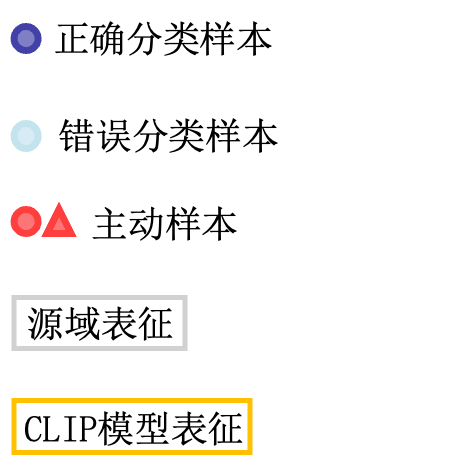
\includegraphics[width=0.23 \linewidth]{figures/chap4/indicator.png}}
    \bicaption[fig:points]{}{目标样本点在表征空间中的 t-SNE 可视化}{Fig.}{t-SNE visualization of the target sample points in the representation spaces}
\end{figure}


表~\ref{tab:ablation_sampling}对比了不同主动样本选择策略在有/无ViL模型监督下的性能：（1）不使用ViL模型时，MH Points在源模型假设空间下表现最优；（2）引入ViL模型后，仅依赖不确定性或多样性的策略（如ELPT、MH点集）甚至低于随机采样，而Core-Set和本章提出的DFSelector组合高于其他策略。这表明在多模型协作框架下，样本选择需同时兼顾双假设空间的几何覆盖与边界信息。
图~\ref{fig:points}给出了Office-Home 数据集 $C\xrightarrow{}P$ 任务上，不同采样策略下主动样本在源模型特征空间中的t-SNE分布~\cite{van2008visualizing}。可见ELPT样本集中于决策边界附近但多样性不足，Core-Set样本分布均匀但偏向类内中心，MH Points同时兼顾边界性与多样性。本章的DFSelector通过加权组合$\mathcal{T}_{\text{MH}}$（关注边界）与$\mathcal{T}_{\text{CO}}$（关注$\mathcal{Z}$空间覆盖），实现了双假设空间下的最优样本分布。



\begin{figure}[!htbp]
    \centering
    \setlength{\tabcolsep}{0pt}
    \subfigure[]{
    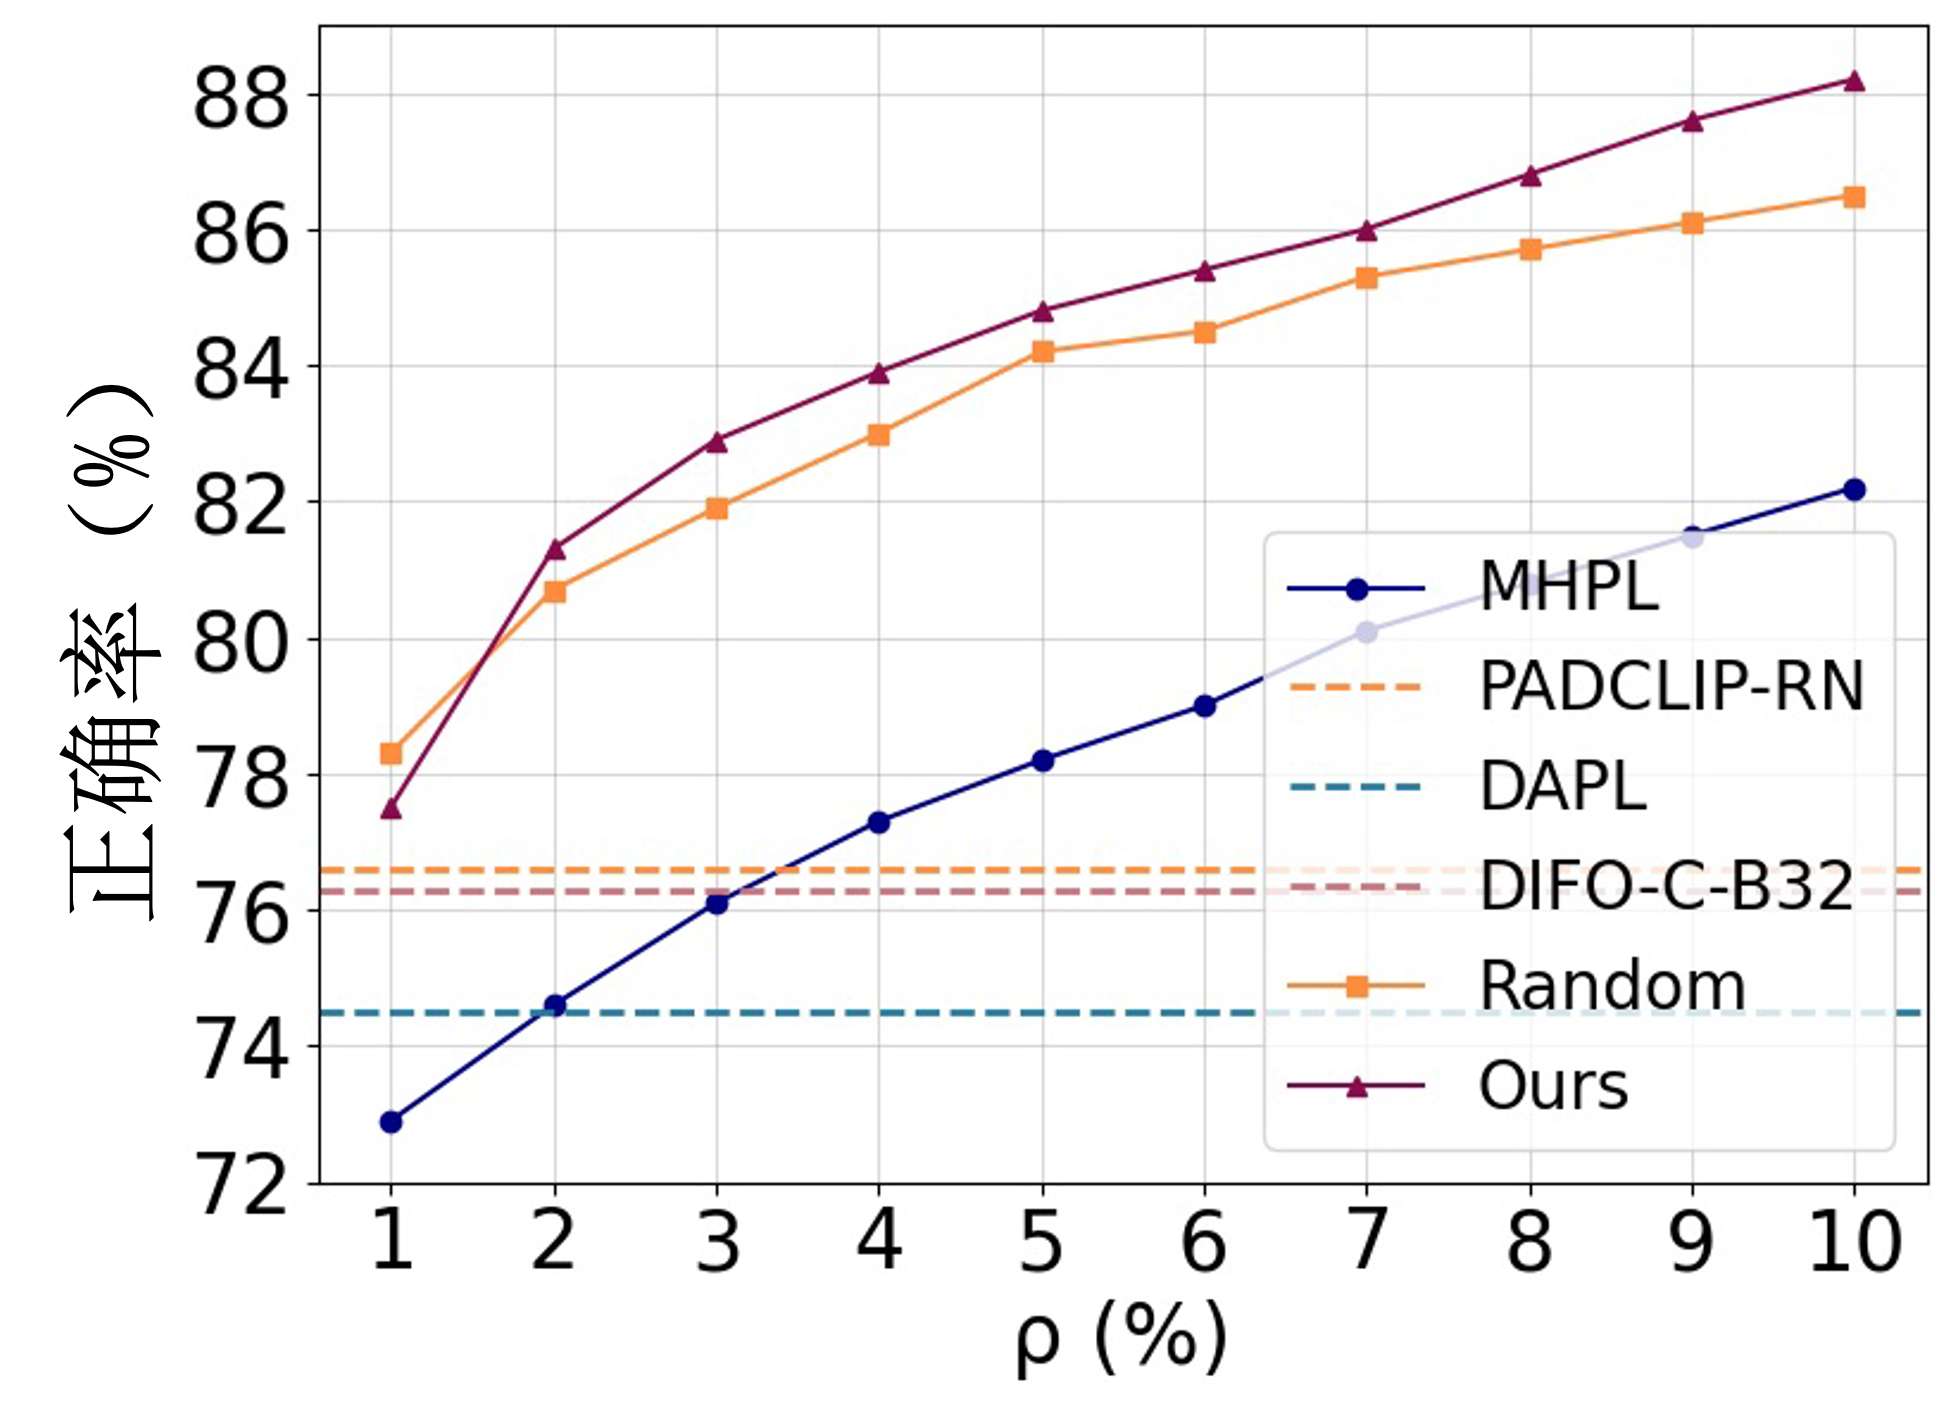
\includegraphics[width=0.3\linewidth]{figures/chap4/abl_active_ratio_uda.png}
        \label{fig:budget_compare}
    }
    \subfigure[]{
    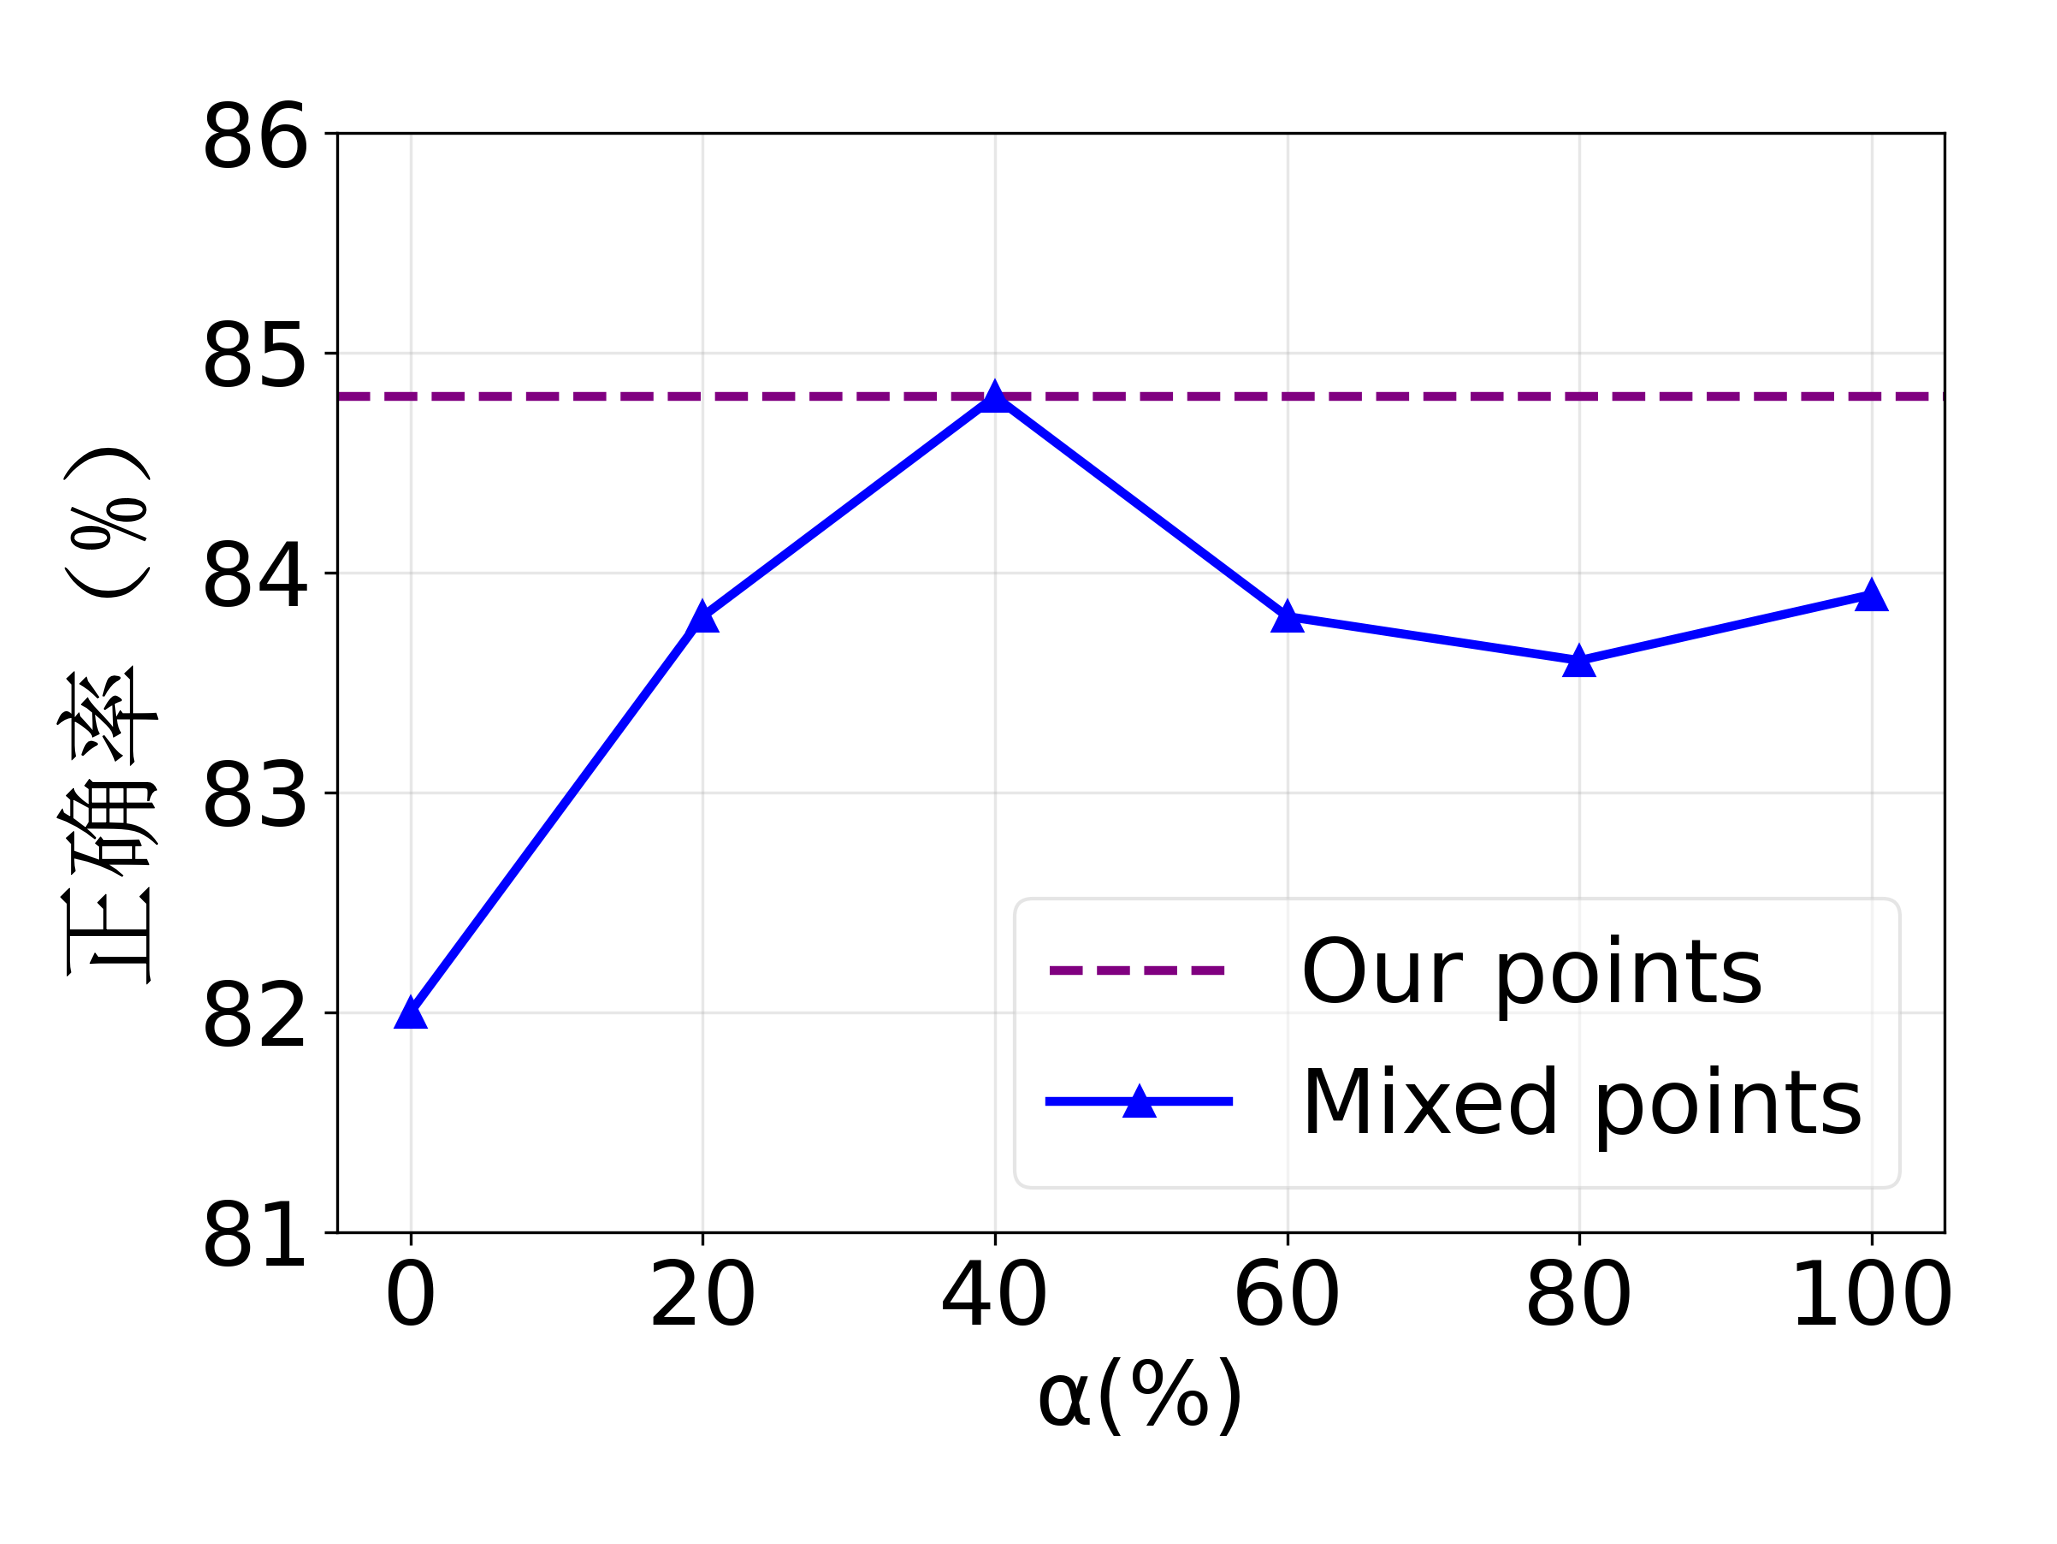
\includegraphics[width=0.3\linewidth]{figures/chap4/mixed_model_alpha_re.png}
        \label{fig:sub_alpha_analysis}
    }
    \subfigure[]{
    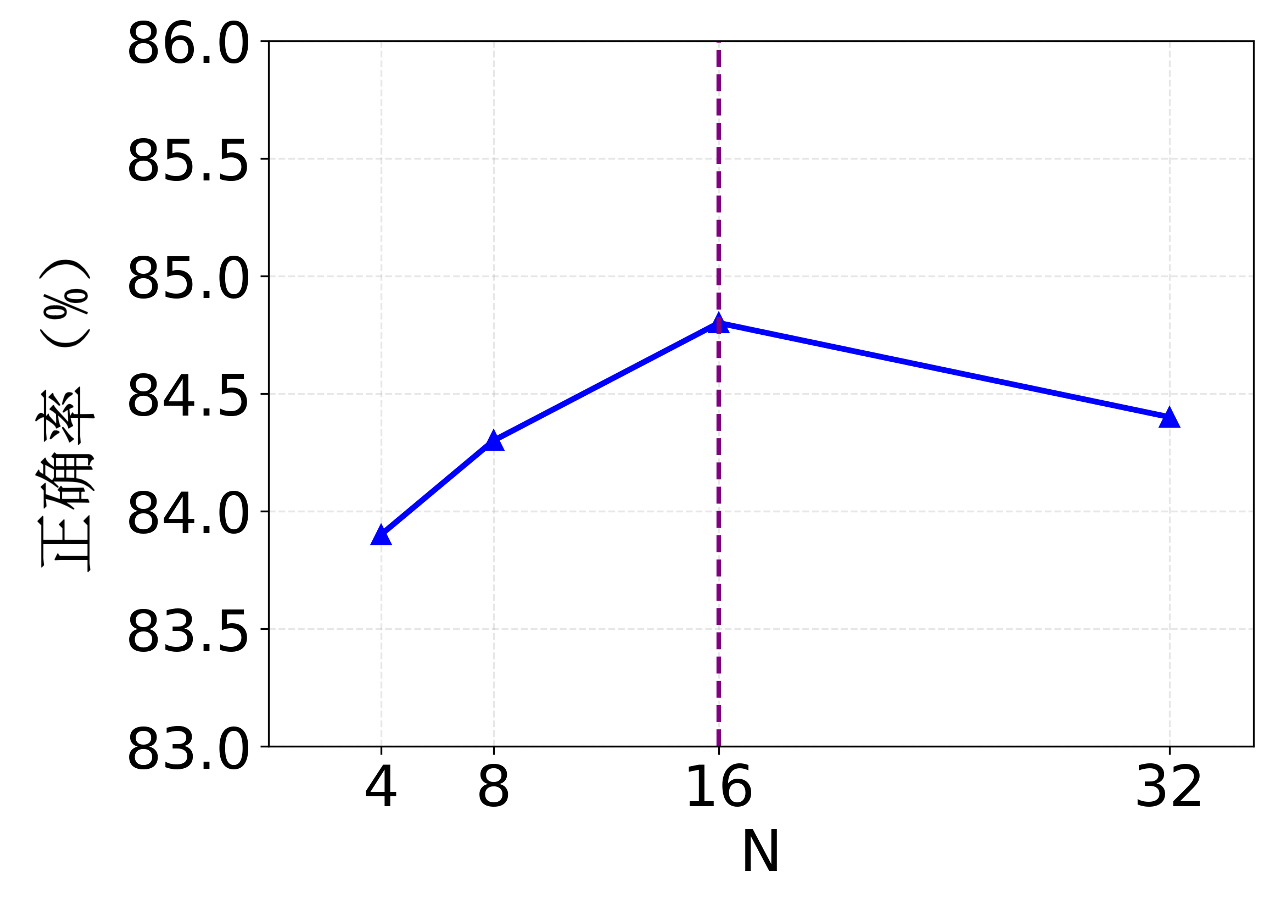
\includegraphics[width=0.3\linewidth]{figures/chap4/accuracy_curve.png}
        \label{fig:abl_n}
    }
\bicaption[fig:alpha_analysis]{}{Office-Home数据集上的参数消融对比}{Fig.}{Parameter ablations on the Office-Home dataset}
\end{figure}


图~\ref{fig:alpha_analysis}包含三组实验，子图（a）对比了DAMF在不同标注预算下的性能表现。DAMF在$\rho\in\{1\%,2\%,5\%,10\%\}$各档预算下均高于基线方法MHPL~\cite{wang2023mhpl}与随机采样基线（Random+DAMF），验证了DFSelector在不同标注预算下的有效性。当标注预算极低时（$\rho=1\%$），DAMF相对MHPL仍保持正向差距，说明其对低资源场景具有一定的适应性。
子图（b）给出$\mathcal{T}_{\text{CO}}$与$\mathcal{T}_{\text{MH}}$加权比例$\alpha$对性能的影响。性能在$\alpha=0.4$处达到峰值，与主实验所报告的性能水平一致；越过该最优点后性能下降并最终趋于平台。该结果印证了$\mathcal{T}_{\text{CO}}$与$\mathcal{T}_{\text{MH}}$两类样本贡献之间的权衡关系：$\alpha$过大时标注集偏向$\mathcal{Z}$空间的几何覆盖而缺乏$\mathcal{X}$空间的边界信息，过小则偏向边界信息捕获而忽略ViL模型的适配需求，因此中间取值构成最优配置。
子图（c）分析目标样本选择大小$N$的影响，即式\eqref{eq:topX}所涉$\mathcal{X}_{\text{top}}$集合中每类保留的高置信样本数。当$N$从4增至32时性能先升后降，在$N=16$处取得峰值。过小的$N$将蒸馏目标限制在极少数高置信样本上，削弱了知识传递信号；过大的$N$则引入噪声预测，破坏ViL模型的对齐质量。据此本文将$N=16$设为全部实验的默认取值。

\noindent\textbf{（3）知识保持正则项的影响}

图~\ref{fig:lambda_sensitivity}给出了知识保持正则系数$\lambda$的影响：闭集场景下$\lambda=1$最优，开放集场景下$\lambda=8$最优。这是因为开放集任务中保留ViL模型的泛化能力对未知类别检测尤为关键。图~\ref{fig:beta_sensitivity}给出了样本权重$\beta_q$与$\beta$的影响：较高的$\beta_q$有助于突出真实标注样本的贡献，而$\beta$在0.3附近表现最佳，过大或过小均会因过度利用或抑制伪标签而损害性能。


\begin{figure}[!htbp]
    \centering
    \subfigure[闭集]{
    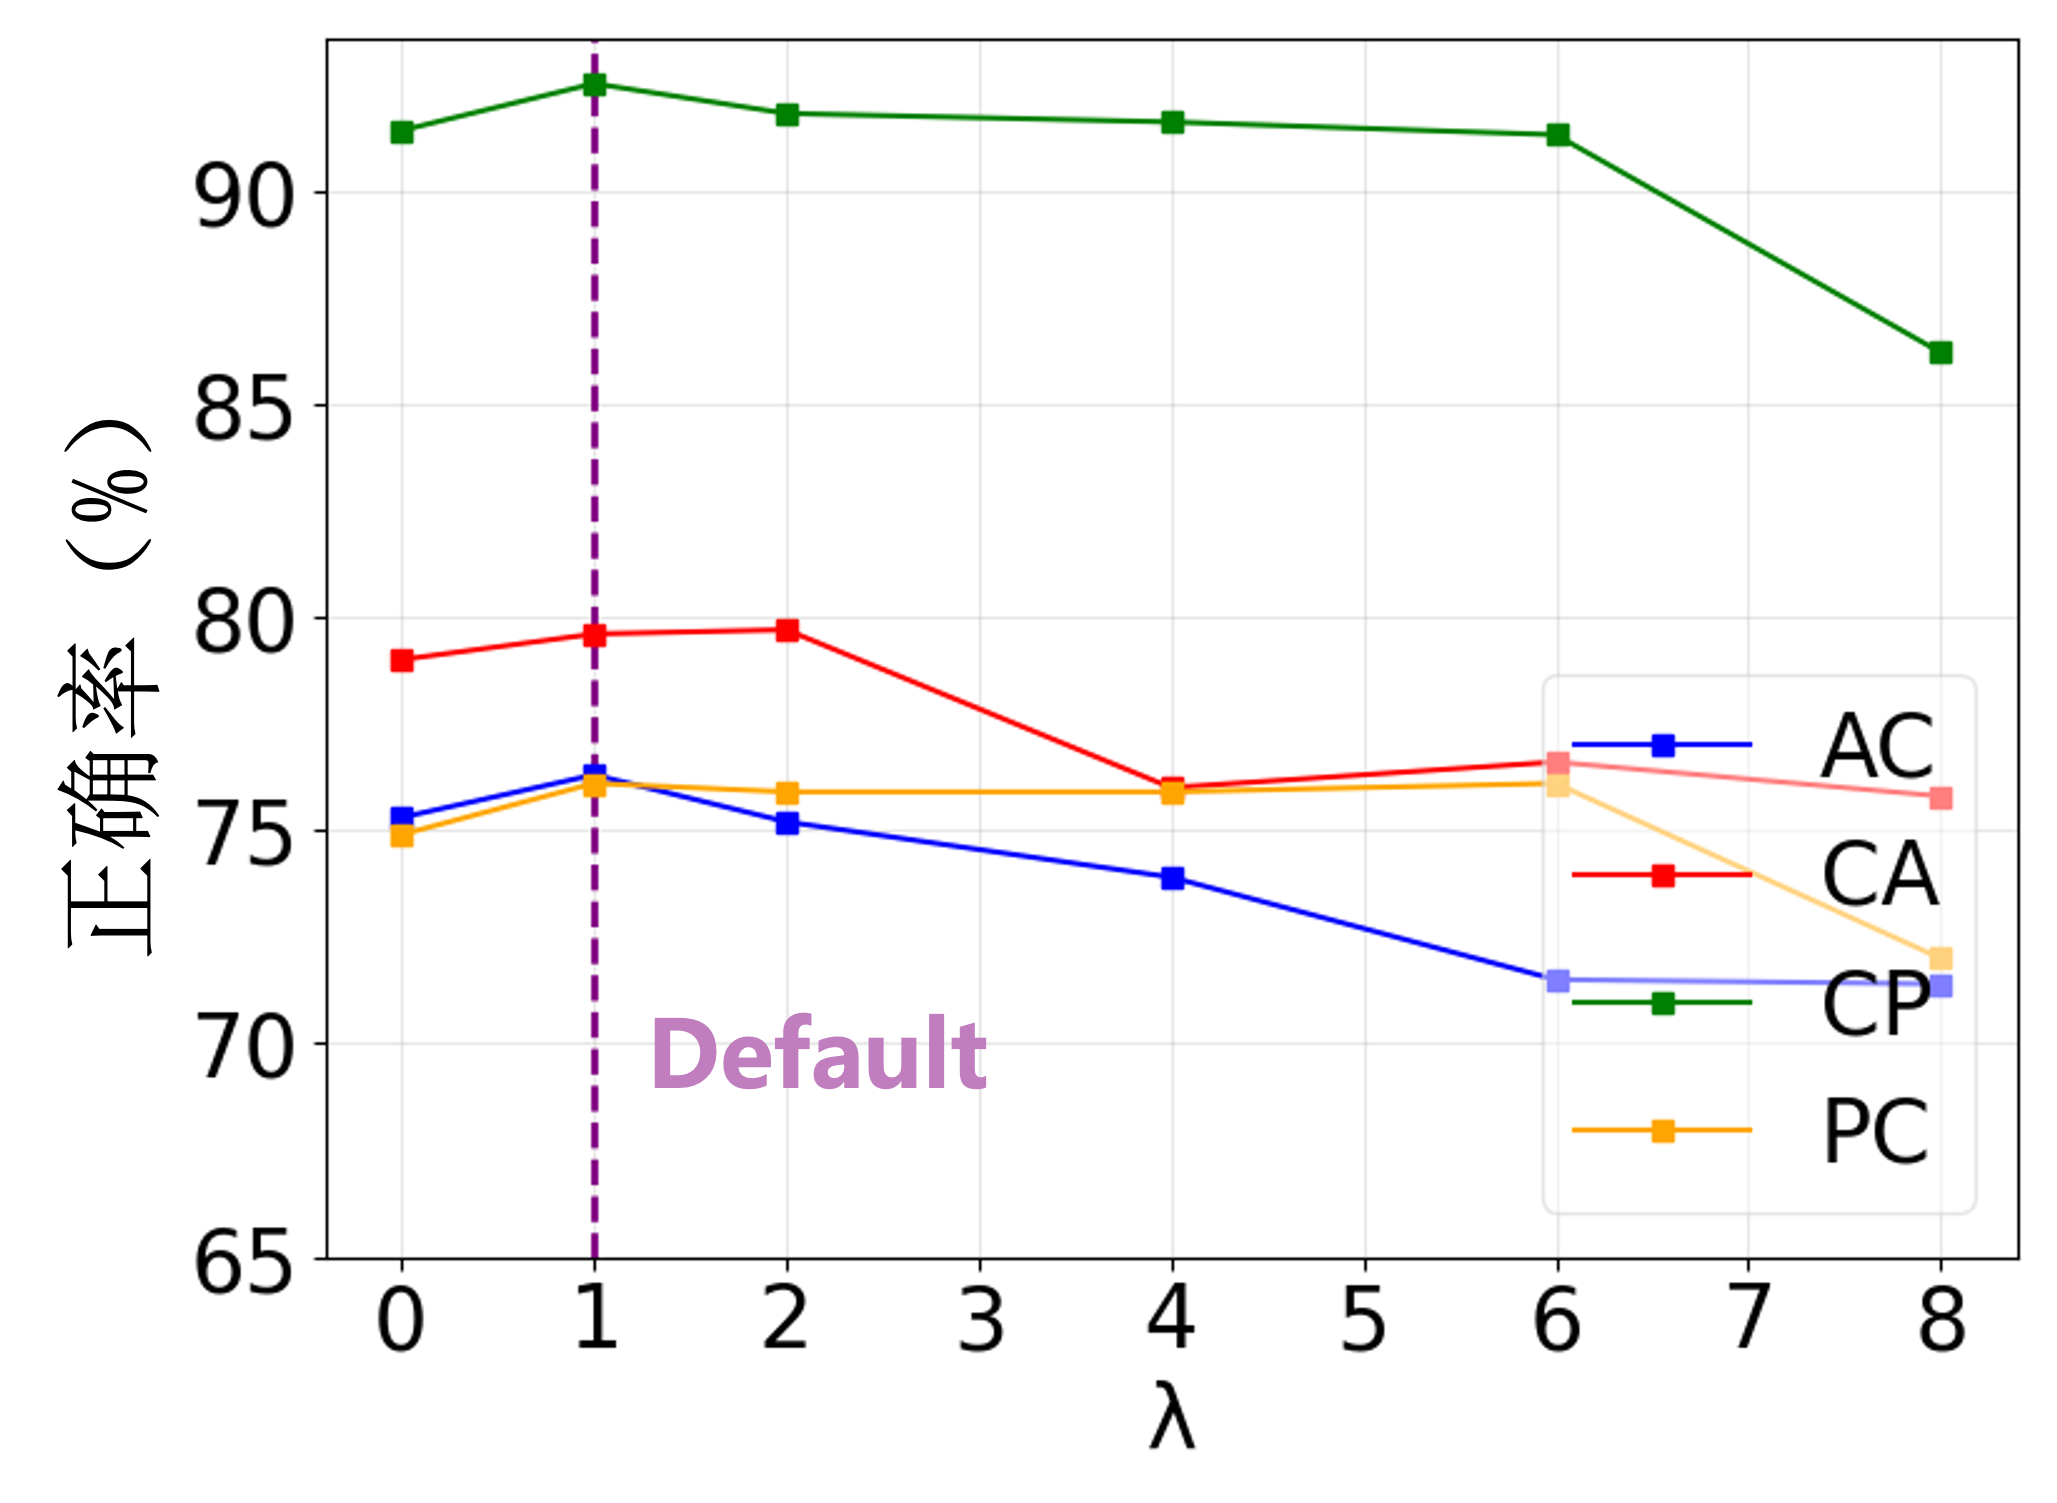
\includegraphics[width=0.35\linewidth]{figures/chap4/uda_lambda.png}}   
    \subfigure[开集]{
    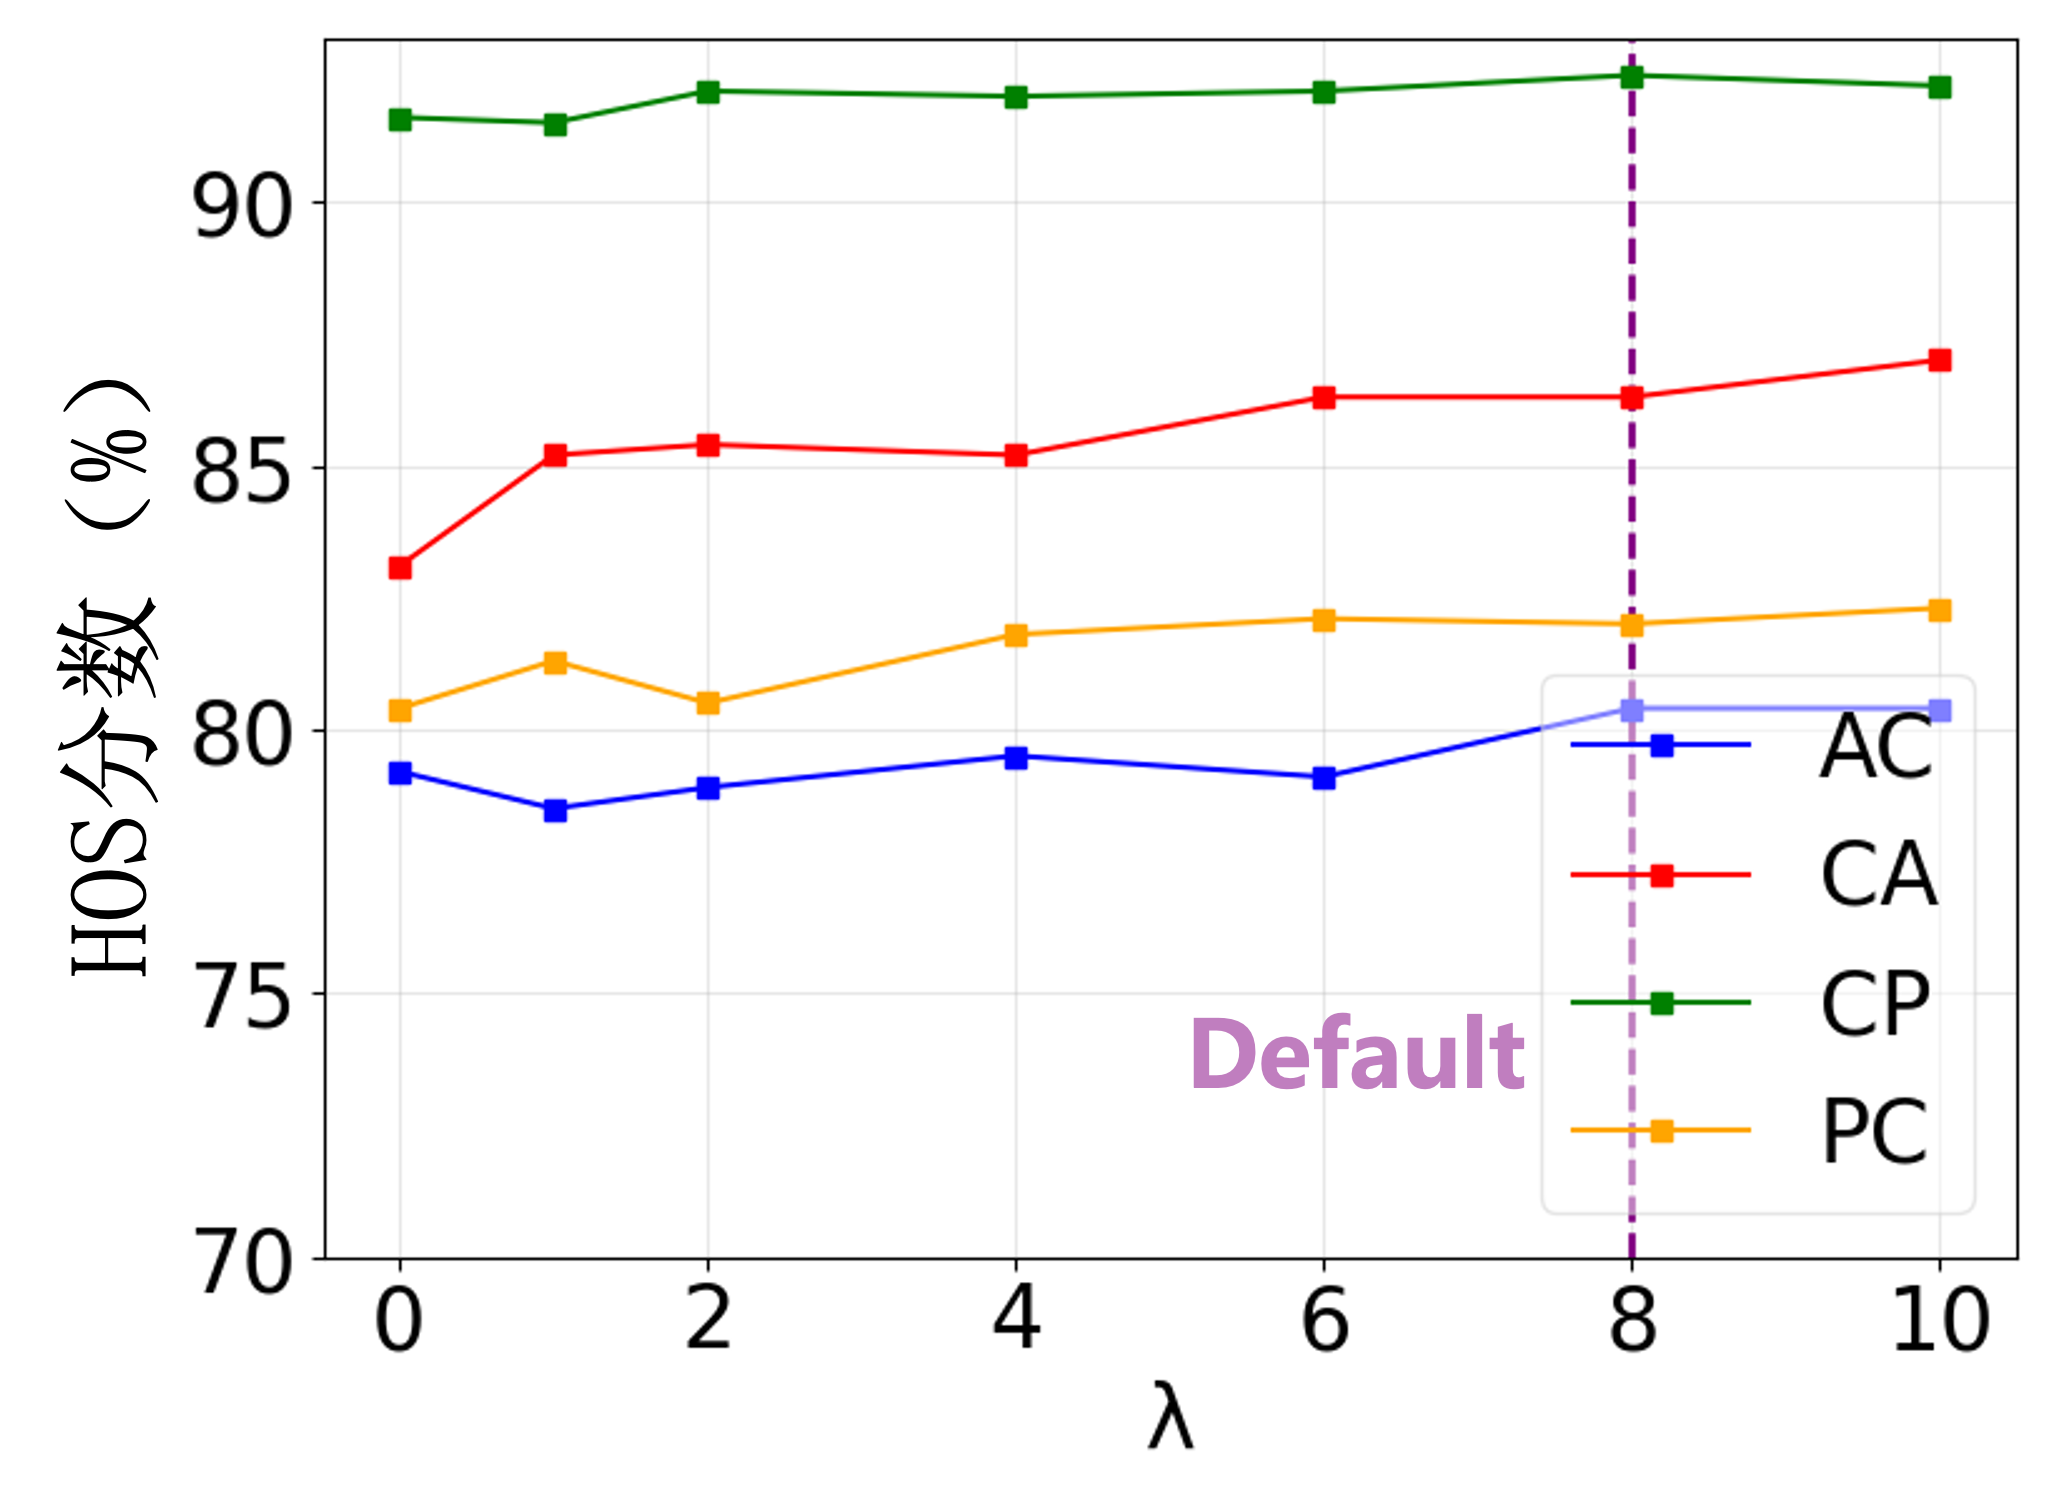
\includegraphics[width=0.35\linewidth]{figures/chap4/oda_lambda.png}}
    \bicaption[fig:lambda_sensitivity]{}{正则系数$\lambda$消融}{Fig.}{Impact of regularization weight $\lambda$}
    \label{fig:lambda}
\end{figure}

\begin{figure}[!htbp]
    \centering
    \subfigure[]{
    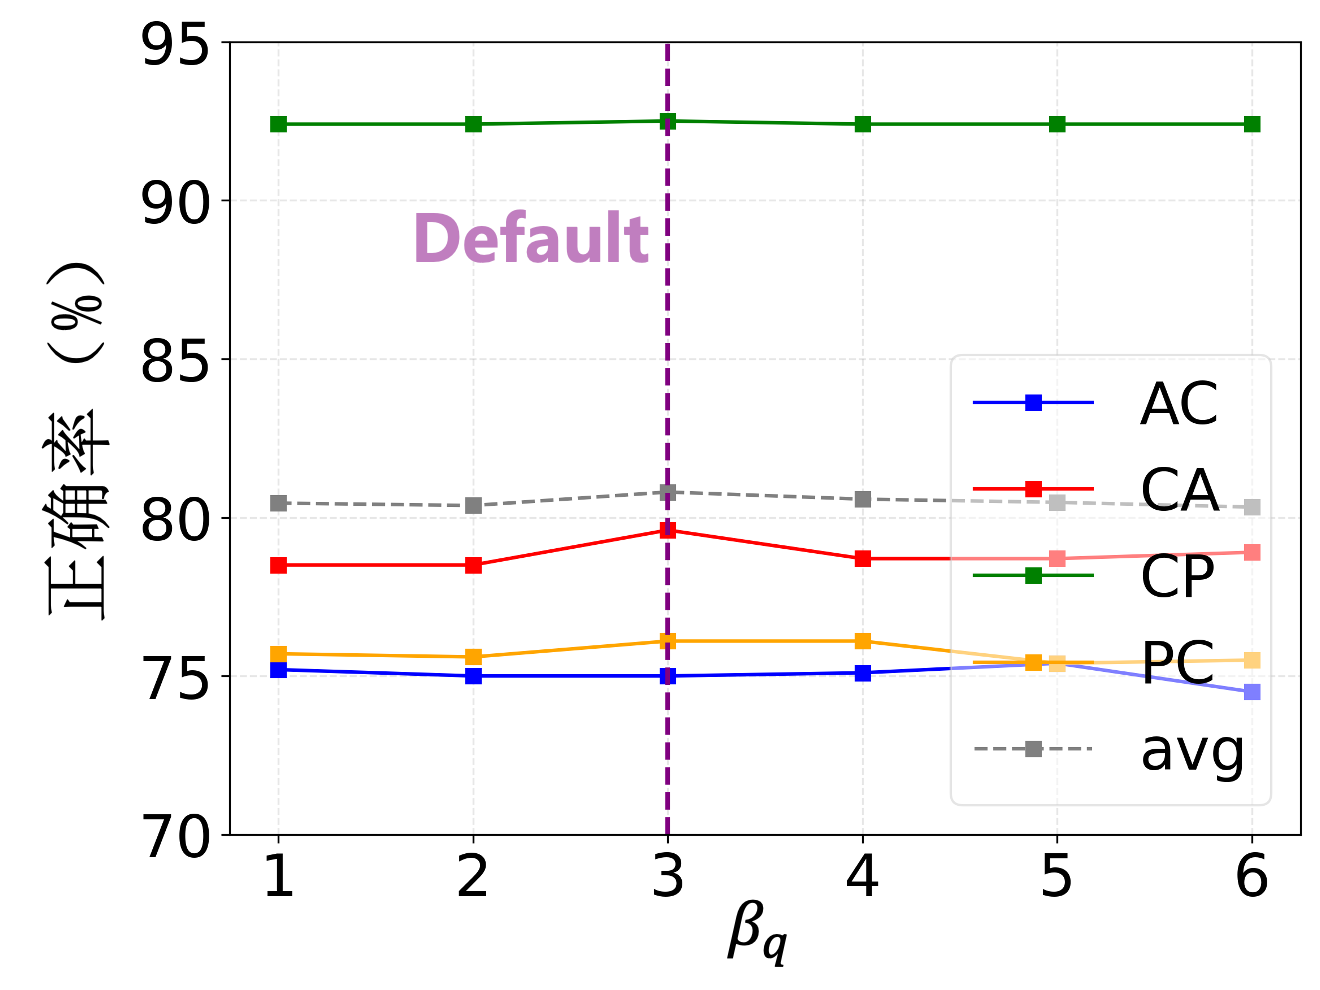
\includegraphics[width=0.35\linewidth]{figures/chap4/abl_betaq.png}}   
    \subfigure[]{
    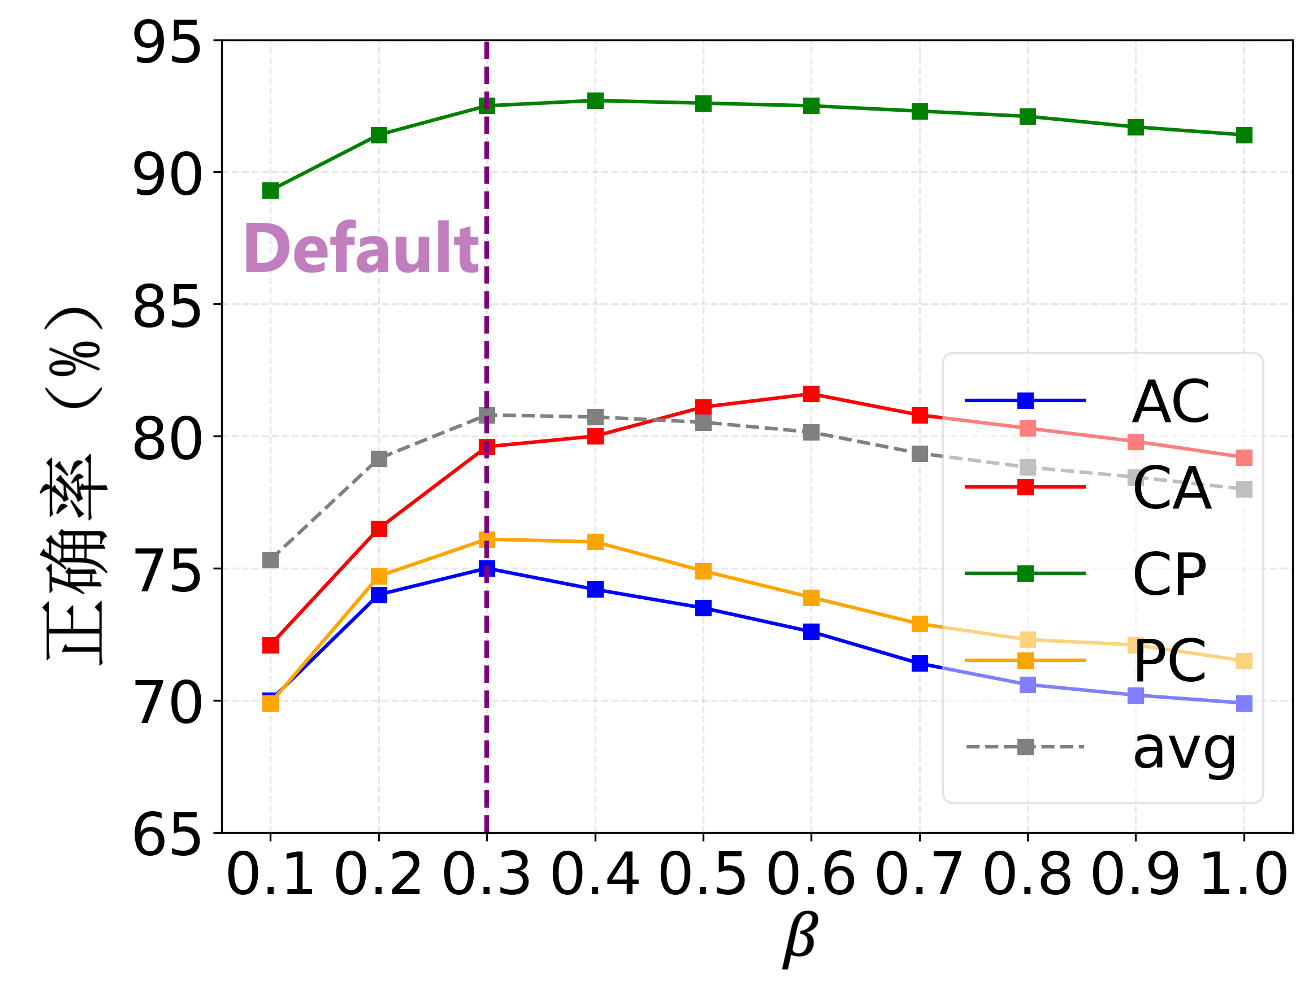
\includegraphics[width=0.35\linewidth]{figures/chap4/abl_beta.png}}
    \bicaption[fig:beta_sensitivity]{}{样本权重$\beta_q$与$\beta$消融}{Fig.}{Ablations of sample weights $\beta_q$ and $\beta$}
    % \caption{Impact of sample weights $\beta_q$ and $\beta$ on the transfer tasks in Office-Home. We report both individual task-wise performance and their average (line 'avg'). The purple dashed line indicates the \textit{Default} setting.}
    \label{fig:beta}
\end{figure}

\noindent\textbf{（4）ViL模型性能分析}

表~\ref{tab:clip_evolution}给出了ViL模型（CLIP）在适应过程中的性能演化。结果显示，CLIP在APT阶段（CUS-C-B32）已获得显著增益，表明主动标注样本对CLIP的类别prompt适配极具价值；进一步经ADL蒸馏后（DAMF-ViL），CLIP性能继续提升。然而DAMF-ViL仍低于完整DAMF，说明ViL模型与目标模型的协作能够实现1+1>2的协同效应。

\begin{table}[!htbp]
    \bicaption[tab:clip_evolution]{}{适应过程中CLIP的准确率演化}{Table}{CLIP accuracy evolution throughout adaptation}
    \vspace{0.5em}\centering\wuhao
    % \resizebox{.9\textwidth}{!}{
    \begin{tabular}{lcccc}
    \toprule
    方法 & Office-Home & VisDA-C & Office & miniDomainNet \\
    \midrule
    ZS-C-B32 & 72.2 & 87.2 & 79.5 & 80.0 \\
    CUS-C-B32 (使用APT后) & 80.0 (+7.8) & 90.2 (+3.0) & 80.9 (+1.4) & 83.5 (+3.5) \\
    DAMF-ViL (使用ADL后)  & 81.7 (+1.7) & 92.1 (+1.9) & 88.8 (+7.9) & 84.0 (+0.5) \\
    \bottomrule
    \end{tabular}  
    % }
\end{table}


% 表~\ref{tab:cost}对比了有无ViL模型情况下的训练与推理开销。DAMF在训练阶段仅增加0.002M可训练参数（prompt参数）和0.48 GB GPU显存（+8.8\%），额外计算量可忽略。闭集推理阶段ViL模型被完全丢弃，对推理速度无影响；开放集推理阶段虽然需要额外调用ViL模型进行未知类别检测，但相比基于聚类的开放集方法（如MHPL-O的2-类k-means聚类），DAMF无需任何预处理时间，反而实现了更高的推理吞吐（339.74 FPS vs 212.68 FPS）。

% \begin{table}[!htbp]
%     \bicaption[tab:cost]{}{训练与推理开销对比}{Table}{Training and inference cost comparison}
%     \vspace{0.5em}\centering\wuhao
%     \begin{tabular}{cccc}
%     \toprule
%     \multirow{2}{*}{ViL} & \multicolumn{2}{c}{训练} & 推理（开放集） \\
%     \cline{2-4}
%     & 可训练参数 [M] & 峰值显存 [GB] & FPS \\
%     \midrule
%     $\times$ & 24.041 & 5.43 & 212.68$^\dagger$ \\
%     \checkmark (本章) & 24.043 (+0.002) & 5.91 (+0.48) & 339.74 \\
%     \bottomrule
%     \end{tabular}
% \end{table}

\FloatBarrier
\section{本章小结}

本章围绕视觉—语言基础模型与稀缺主动标注难以有效协同的问题，沿样本筛选与跨模型协同两个角度协同推进。在样本筛选层面，借助双假设空间下的样本覆盖度量选择最具信息量的目标样本，突破简单组合框架下的性能瓶颈；在跨模型协同层面，借助任务感知的提示激活与双向知识互补机制实现视觉—语言模型与目标模型之间的稳定融合，避免视觉—语言模型丧失泛化能力。理论层面，本章推导了 SFADA 协作风险上界，明确了双假设空间下的样本覆盖、视觉—语言模型的目标域风险与跨模型对齐损失三个关键因素的协同优化目标。实验在闭集与开放集两种设定下均取得当前最优性能，验证了所提框架的有效性与工程实用性，并为下一章在开放类设定下将视觉—语言模型的开放语义与分割基础模型的空间定位能力进一步深度融合奠定了双模型协同的框架基础。

% Local Variables:% Local Variables:
% TeX-master: "../thesis"
% TeX-engine: xetex
% End:

% !Mode:: "TeX:UTF-8"

\chapter[基于多流语义对齐融合的开放类泛化]{基于多流语义对齐融合的开放类泛化}[]
\chaptermark{基于多流语义对齐融合的开放类泛化}

\label{chap:4}
\thispagestyle{plain}
\section{引言}

跨类泛化是模型迁移研究在类别词表维度上的关键挑战，其核心要求是模型对训练阶段未见过的新颖类别保持识别能力。在密集预测任务中，这一要求体现为两个相互关联的方面：模型须为新类别给出正确的语义判别，并须在像素层面准确界定该类别的区域归属。前者要求判别依据不依附于固定类别索引，后者在训练仅覆盖有限类别时更为困难：新类别在训练阶段没有对应的像素级监督，模型倾向于将目标区域错误归入相近的已见类别。跨类泛化的研究重心，因而落在如何以多流先验的协同弥补单一语义来源在密集预测能力上的缺口。

近年来，大规模视觉—语言预训练模型在通用视觉理解任务上取得了长足进展~\cite{yin2023vlp}，其中 CLIP~\cite{radford2021learning} 与 ALIGN~\cite{jia2021scaling} 通过对比学习在海量图文对上建立了视觉与语言的联合嵌入空间，赋予模型强大的零样本泛化能力~\cite{radford2021learning,zhou2022learning}。然而，这类模型的预训练过程缺乏像素级标注，难以直接生成高质量的密集预测~\cite{rao2022denseclip}。相反，分割基础模型 SAM~\cite{kirillov2023segment} 通过大规模分割数据训练，在零样本实例分割任务上表现出色，但其本身缺乏语义理解能力。两种基础模型具有天然的互补特性：CLIP 擅长开放词汇语义识别，SAM 擅长像素级空间定位，为跨类泛化研究提供了多模态类别先验的协同来源。

现有跨类泛化方法在多流语义对齐与空间定位两个层面均存在不足。在多流语义对齐层面，现有方法主要分为两阶段与单阶段两种范式：两阶段方法~\cite{liang2023open,ding2022decoupling,xu2022simple} 通常先由额外的分割模型生成类别无关的掩码提议，再借助 ViL 模型对其进行分类，该范式存在两方面局限——掩码提议与分类过程分离导致两者所依赖的特征不对齐，且类别无关的掩码生成过程效率较低、对未见类别的掩码质量不佳；单阶段方法如 FC-CLIP~\cite{yu2023convolutions} 以 CLIP 的图像编码器为骨干端到端生成掩码提议，虽然简化了流程并缓解了提议过拟合，但其掩码质量仍受限于 CLIP 本身在像素级对齐方面的固有局限。在空间定位层面，上述方案均难以在统一解码框架内充分利用 SAM 的高质量掩码先验，致使对长尾与未见类别的细粒度识别能力受限。

上述缺陷在图~\ref{fig:cmpf_motivation} 中得到了直观体现：左图为 PC-459~\cite{mottaghi2014role} 数据集上现有 SOTA 方法 FC-CLIP 在已见与未见类别上的分割结果对比，FC-CLIP 在未见类别上的分割质量显著弱于已见类别，反映了基于 CLIP 的开放词汇分割方法对未见类别的实质性短板；右图为 CMPF 与 MaskCLIP~\cite{ding2023open}、FC-CLIP 在未见类别上的平均召回率 AR与平均交并比mIoU定量对比，进一步表明现有 CLIP 基方法在未见类别上的识别能力存在系统性不足。尽管近期工作通过类别无关掩码学习~\cite{liang2023open,dou2022learning} 与教师—学生自训练~\cite{xu2023learning} 等策略尝试缓解该问题，但均未能从根本上解决基于统一解码框架的多流语义对齐与空间定位深度融合这一核心难题。

\begin{figure}[!htbp]
    \centering
    \subfigure[]{
    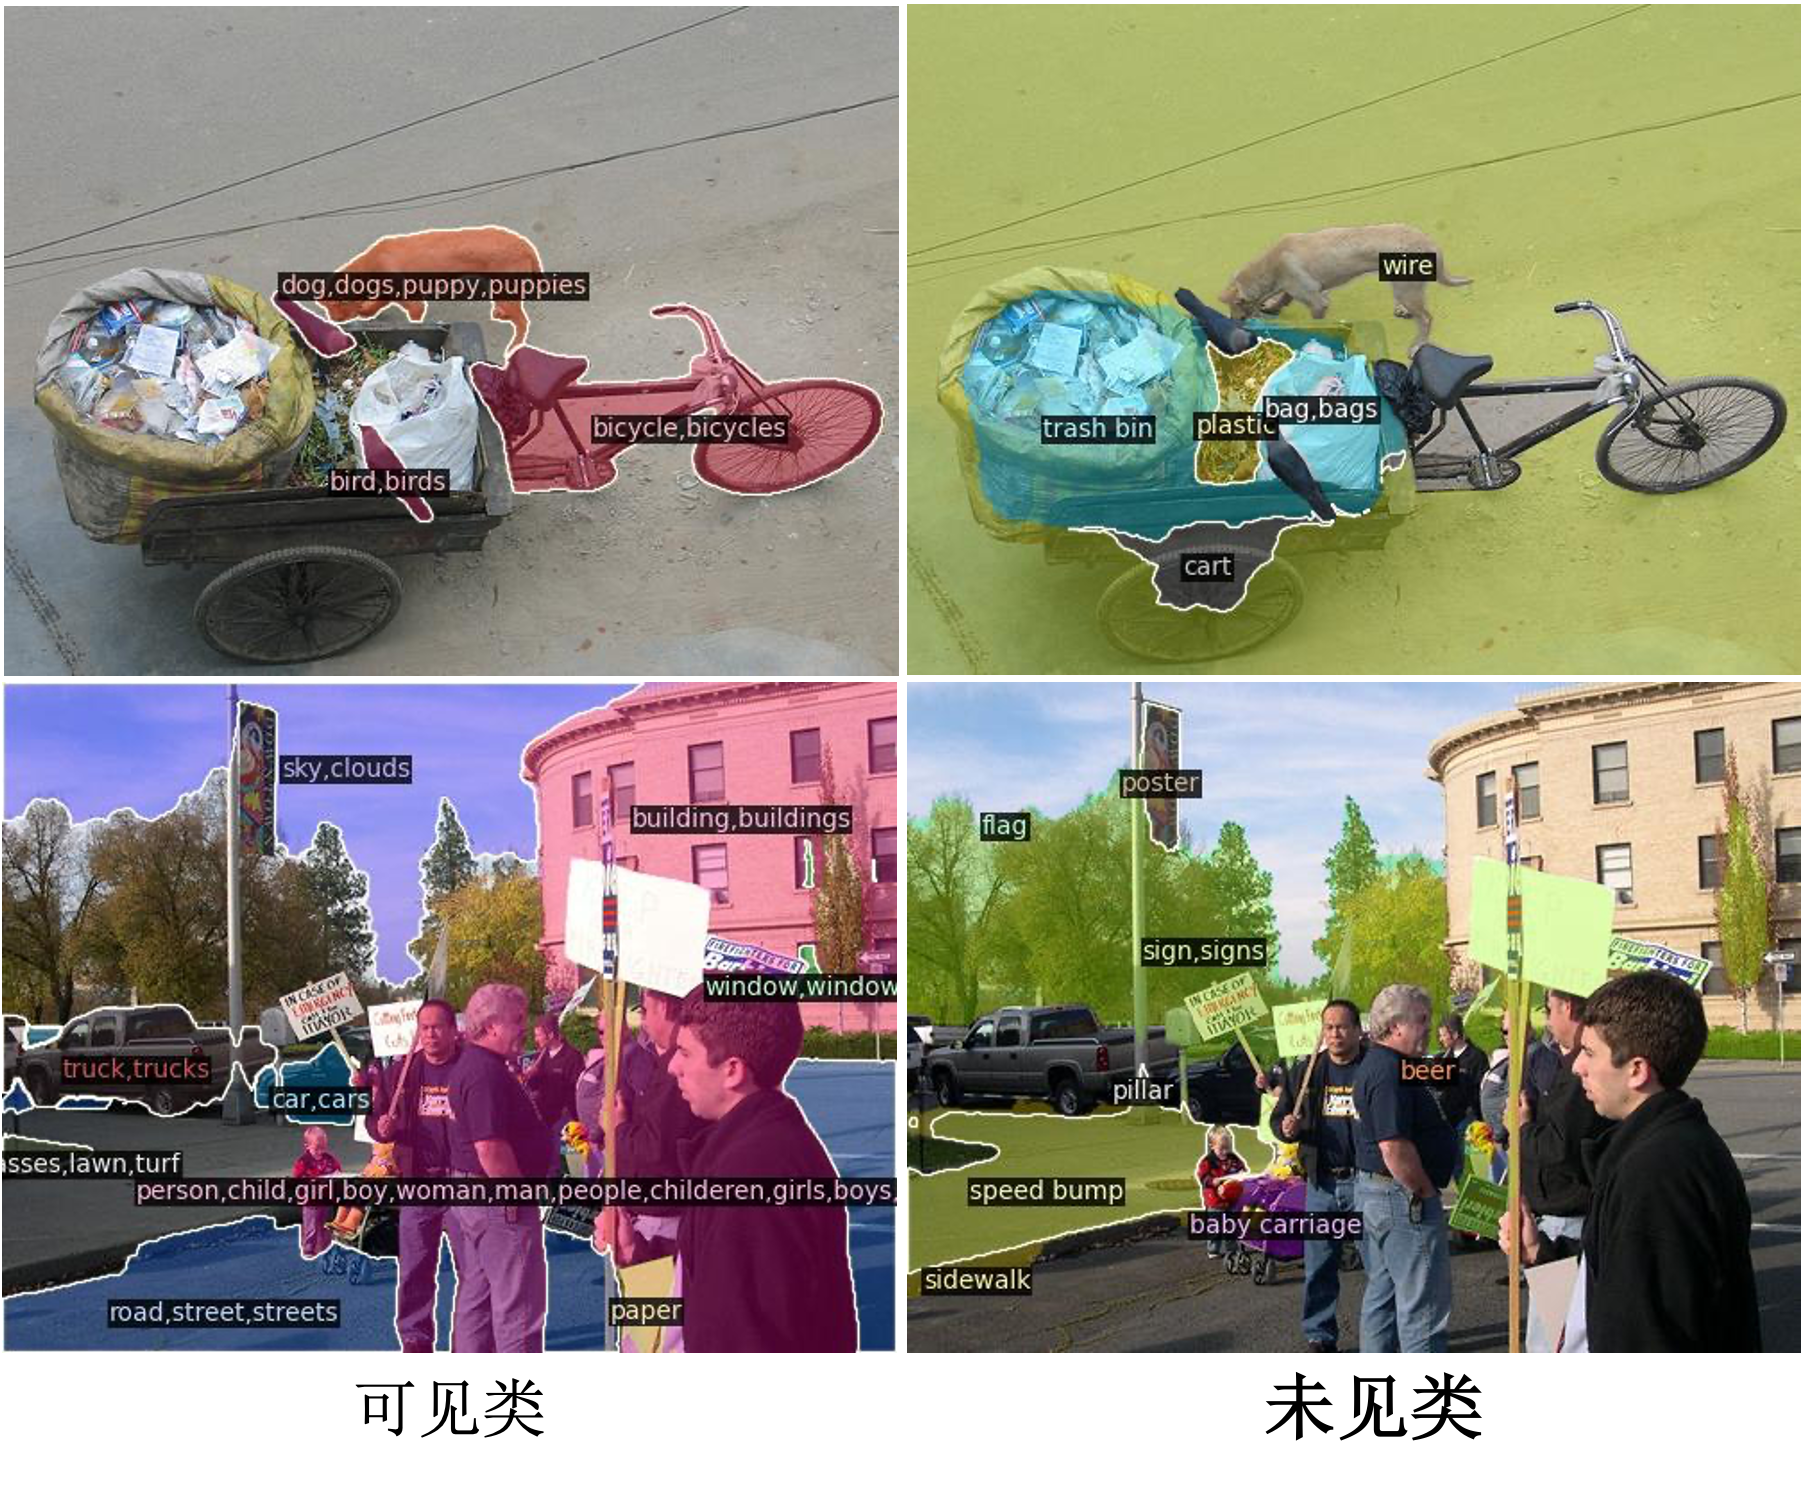
\includegraphics[width=0.58\textwidth]{figures/cmpf/moti_a.png}
    }
    \hfill
    \subfigure[]{
    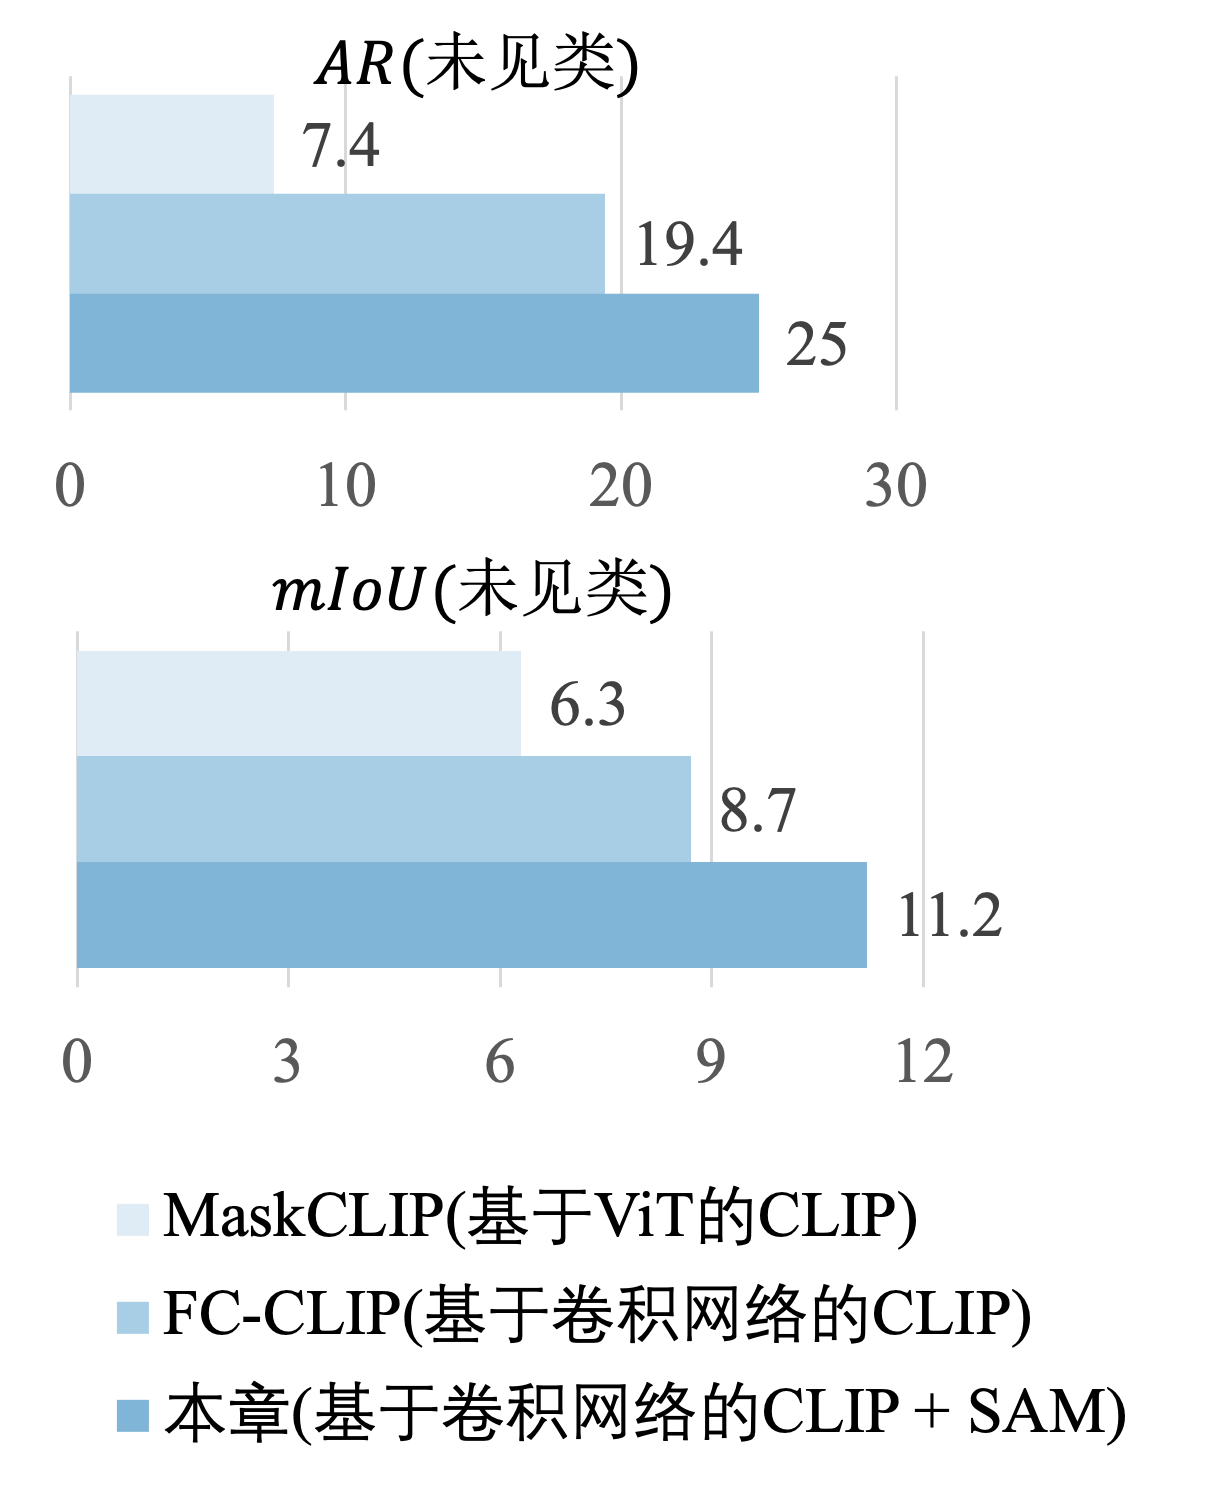
\includegraphics[width=0.38\textwidth]{figures/cmpf/moti_b.png}
    }
    \bicaption[fig:cmpf_motivation]{}{现有开放词汇SOTA方法对已见与未见类别的分割性能对比（左），及本章方法与其他两种方法的AR与mIoU对比（右）}{Fig.}{Comparison of SOTA open-vocabulary segmentation methods on seen vs unseen classes (left) and AR/mIoU on unseen classes (right) of CMPF vs MaskCLIP and FC-CLIP on PC-459}
\end{figure}

为突破上述瓶颈，本章提出基于跨模型先验融合的开放词汇分割方法 CMPF。该方法的核心思想是：协同整合SAM的像素级空间定位能力与CLIP的开放词汇语义理解能力，通过查询注入器与特征注入器两个模块在Transformer解码器内部实现两类先验知识的深度融合，并借助开放集合集成模块在推理阶段融合SAM的零样本掩码预测，进一步提升未见类别的分割质量。

本章的主要贡献可总结为以下三点：
\begin{enumerate}
    \item CMPF 跨模型先验融合框架：在 Mask2Former~\cite{cheng2021masked} 基础上首次系统性融合 SAM 的视觉定位先验与 CLIP 的语义先验，实现两类基础模型在开放词汇分割任务上的协同优化。
    \item Query Injector 与 Feature Injector：两个轻量化的注入器模块分别从查询与特征两个层面将 SAM 的细粒度空间信息注入 CLIP 驱动的解码器，在保持两个基础模型冻结的前提下提升了掩码提议质量。
    \item OpenSeg Ensemble 推理策略：通过类别集成与掩码集成两阶段融合 SAM 的零样本掩码，进一步增强对未见类别的分割泛化能力。
\end{enumerate}


\section{基于双流特征融合的开放词汇分割}

\begin{figure}[!htbp]
    \centering
    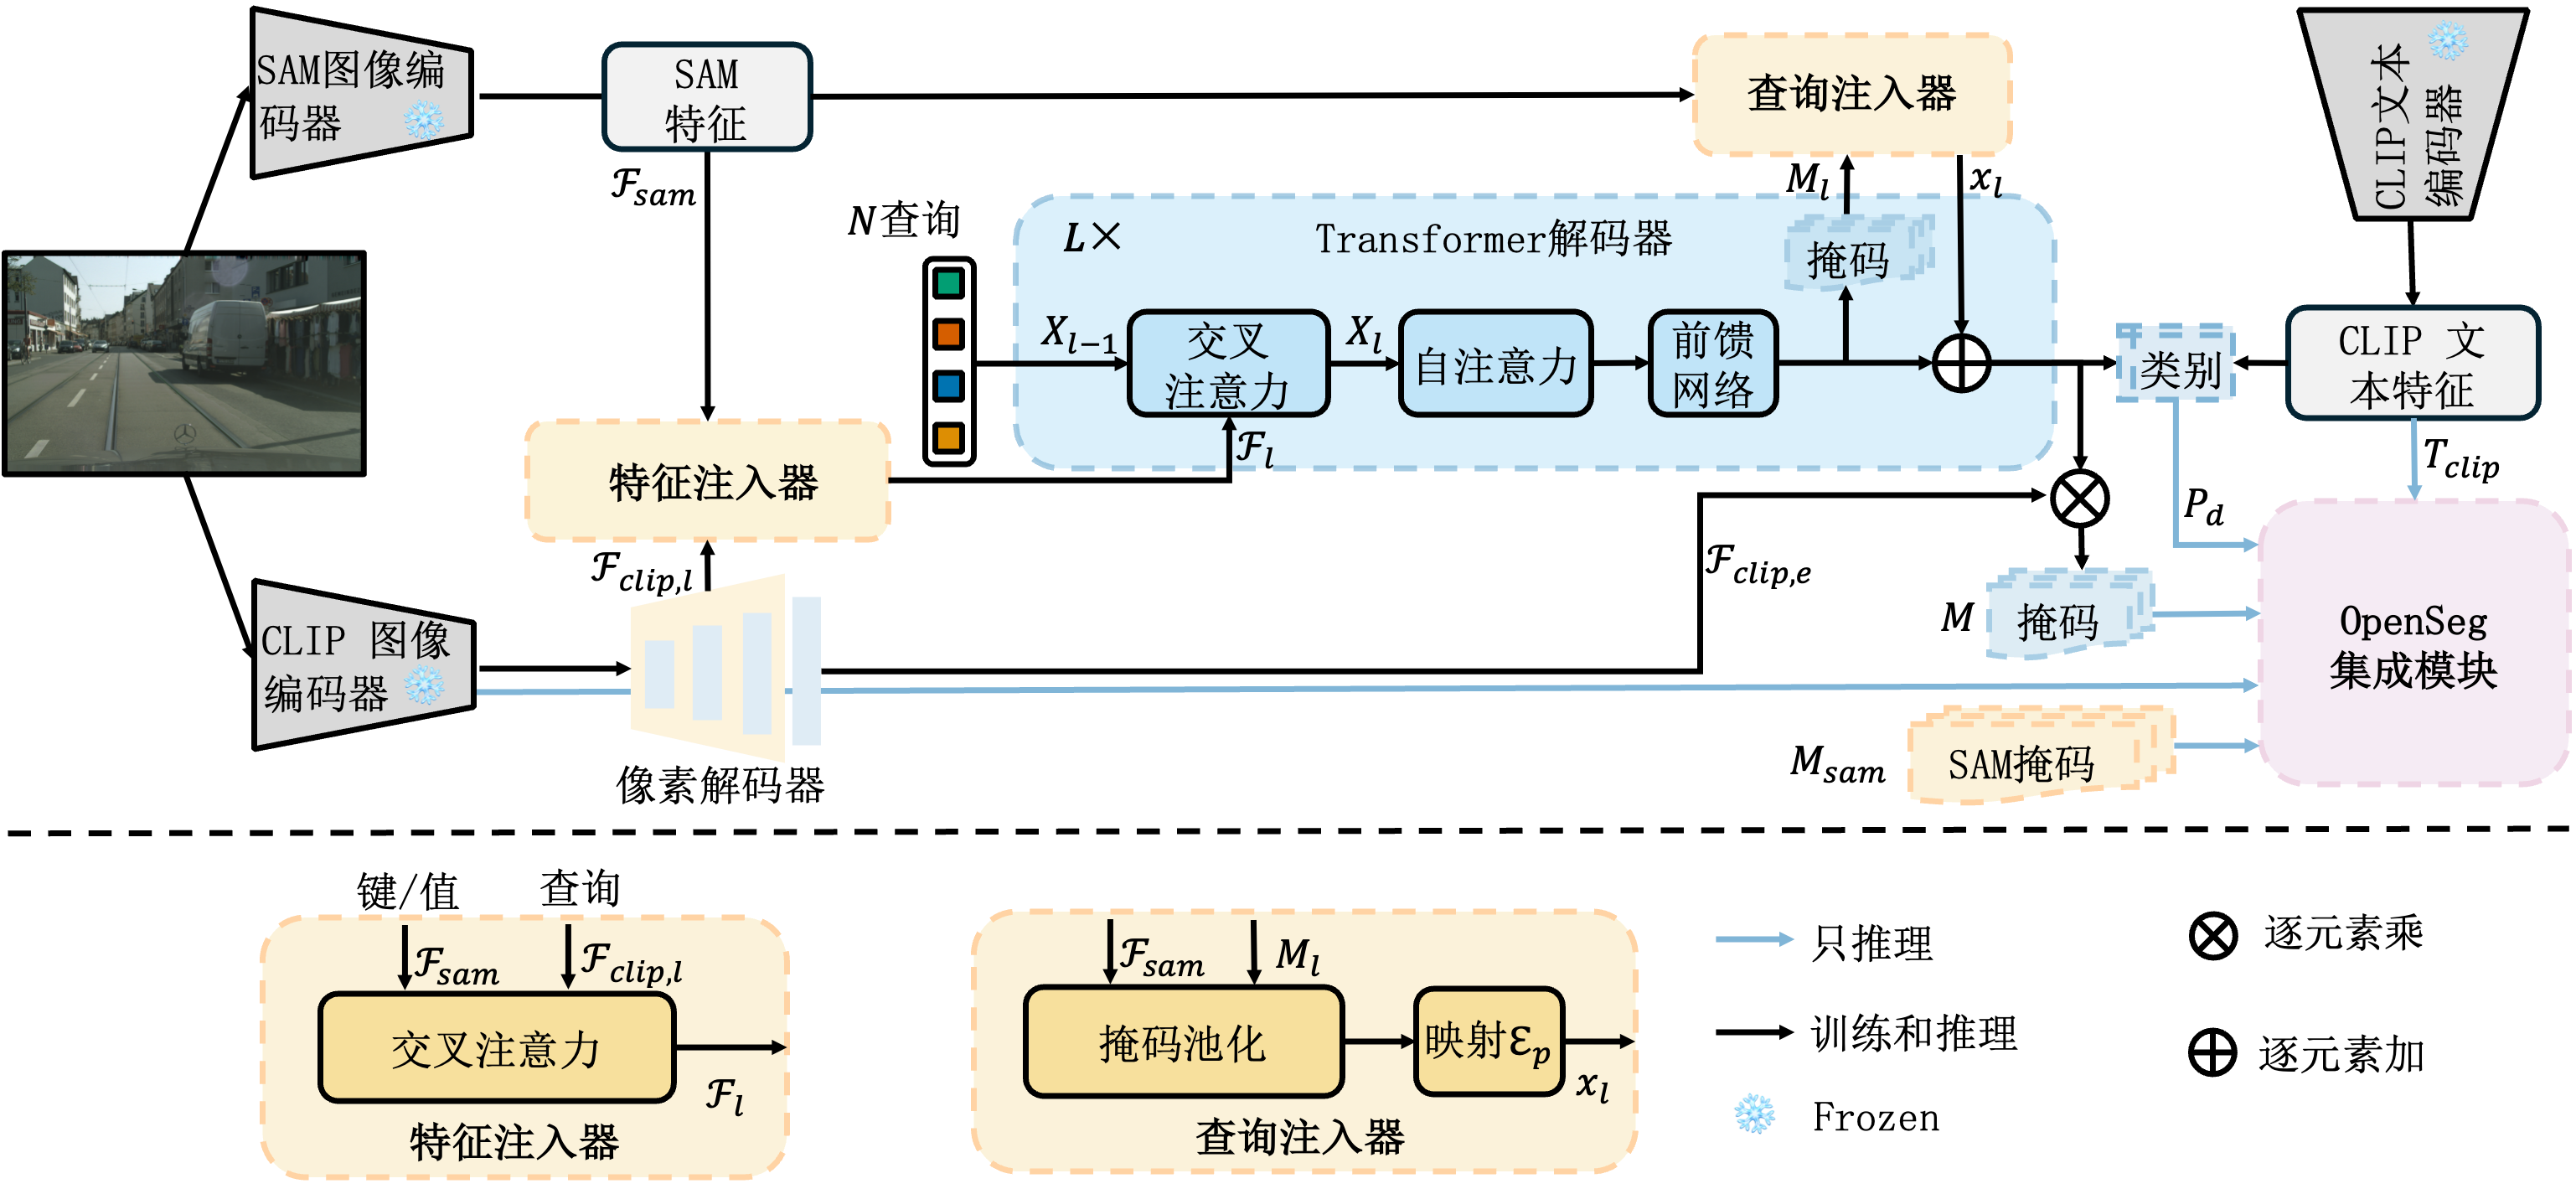
\includegraphics[width=0.95\textwidth]{figures/cmpf/frozen_framework.png}
    \bicaption[fig:cmpf_framework]{}{CMPF总体框架示意图}{Fig.}{Overview of CMPF framework}
\end{figure}

CMPF的总体框架基于Mask2Former~\cite{cheng2021masked}构建。开放词汇分割任务要求模型在训练时使用预定义类别集合 $\mathcal{C}_{\text{train}}$ 对应的真值掩码进行学习，在测试时对包含新类别的 $\mathcal{C}_{\text{test}}$ 进行零样本分割，具体可细分为语义分割（为每个像素赋予语义类别）、实例分割（识别并分割独立的目标实例）与全景分割（同时处理上述两者）。本章框架包含两个并行特征流：CLIP流与SAM流。CLIP的图像编码器作为视觉语义骨干网络，配合像素解码器生成多尺度特征$\{F_{\text{clip},l}\}_{l=1}^{L_{\text{dec}}}$与掩码特征$F_{\text{clip},e}$；SAM的图像编码器并行处理输入图像，生成细粒度空间特征$F_{\text{sam}}$。整个Transformer解码器由$L_{\text{dec}}=9$层组成，每层通过三个核心操作与图像特征交互：与特征图的交叉注意力、查询间的自注意力以及前馈网络变换。解码器维护$N_q$个可学习查询，用于生成候选掩码与类别预测。

% 为有效融合两类基础模型的互补先验，本章在解码器内部设计了两个专门的注入模块：

% \begin{itemize}
%     \item Query Injector：将SAM的细粒度空间特征通过掩码池化与投影转换为空间查询$\{x_l\}_{l=1}^{L_{\text{dec}}}$，并通过元素加法注入到Transformer解码器的可学习查询中，使查询具备空间感知能力；
%     \item Feature Injector：在CLIP特征与查询的交叉注意力之前，借助多头交叉注意力机制（MHCA）~\cite{vaswani2017attention}将SAM的空间细节与CLIP的语义特征融合，使CLIP特征在像素层面更加精细。
% \end{itemize}

% 在推理阶段，CMPF进一步引入OpenSeg Ensemble模块，通过类别集成（融合检测器与CLIP的类别预测）与掩码集成（融合SAM的零样本掩码）两阶段策略提升未见类别的分割精度。两个基础模型在整个训练与推理阶段均保持冻结，训练开销仅集中于轻量化的Transformer解码器。

\subsection{基于多尺度双注入器的掩码查询优化}

\label{sec:chap4_dual_injector}

冻结两个基础模型虽然保留了其预训练知识，但限制了模型捕获细粒度空间信息的能力。具体而言，Transformer解码器中的可学习查询仅依赖CLIP特征进行更新，缺少显式的空间锚定信号。为有效缓解这一问题，本章从查询与特征两个层面分别设计注入模块，实现SAM细粒度空间先验向CLIP驱动解码器的深度融合。

Query Injector（查询注入器）的核心思想是：将SAM的细粒度空间特征转换为空间查询，注入到解码器的查询中。给定Transformer解码器第$l$层新生成的掩码$\mathcal{M}^l$，Query Injector通过掩码池化在SAM特征$F_{\text{sam}}$上提取与当前掩码区域对齐的空间特征，并经过投影函数$E_p$转换为空间查询：
\begin{equation}
x^l = E_p(\mathrm{pool}_{\mathcal{M}^l} F_{\text{sam}}).
\label{eq:query_injector}
\end{equation}

该空间查询专注于掩码所覆盖的前景区域，与可学习查询$X^l$进行元素加法后送入下一解码器层：
\begin{equation}
X^l_{\text{enhanced}} = X^l + x^l.
\end{equation}

这种设计带来两方面优势：（1）空间查询为解码器提供了显式的像素级空间锚定，使查询能够“知道”自己应该关注图像中的哪个区域；（2）注入位置设计为解码器中间层（$l=3,6,9$），既保证查询有足够的时间与CLIP特征进行多轮语义交互，又使后续的解码层能够对新引入的空间信息进行进一步精炼。

Feature Injector（特征注入器）从特征层面进一步提升CLIP的像素级表征能力。该模块借助多头交叉注意力（MHCA）~\cite{vaswani2017attention}机制，在解码器与CLIP特征进行交叉注意力之前，将SAM的空间细节显式地融合到CLIP的图像特征中。Feature Injector首先对CLIP特征进行查询、对SAM特征进行键值投影，然后通过注意力计算生成增强后的CLIP特征：
\begin{equation}
F^l = \mathrm{Softmax}\bigg(\frac{f_q(F_{\text{clip},l})f_k(F_{\text{sam}})^\top}{\sqrt{d_k}}\bigg) f_v(F_{\text{sam}})，
\label{eq:feature_injector}
\end{equation}
其中$f_q$、$f_k$、$f_v$为MHCA的线性投影函数，$\sqrt{d_k}$为缩放因子。为控制计算复杂度，Feature Injector仅在低分辨率特征（$1/32$尺度）上应用，对应解码器的层$l=1,4,7$。

在解码器每一层$l$，模型通过三个投影函数完成预测：（1）$E_m$将查询特征投影为掩码预测的查询嵌入；（2）$E_{aux}$将池化后的掩码特征投影为预测辅助嵌入；（3）$E_c$将查询特征投影为CLIP文本对齐的类别嵌入。掩码预测通过查询嵌入与CLIP掩码特征的乘积生成：
\begin{equation}
\mathcal{M}^l = E_m(X^l) \cdot F_{\text{clip},e},
\label{eq:mask_pred}
\end{equation}
其中$\mathcal{M}^l$为连续掩码值，最终层输出记为$\mathcal{M}=\{m_i\}_{i=1}^{N_q}$。类别预测则通过类别嵌入与CLIP文本特征$T_{\text{clip}}$的对齐计算：
\begin{equation}
P_d = \mathrm{Softmax}\big(E_c(X^l + E_{aux}(\mathrm{pool}_{\mathcal{M}} F_{\text{clip},e})) \cdot T_{\text{clip}}^\top / \tau\big),
\label{eq:class_pred}
\end{equation}
其中$\tau$为可学习的温度参数。解码器采用Masked Attention机制：每层交叉注意力的掩码$\mathcal{M}^{l-1}$由前一层预测计算：
\begin{equation}
\mathcal{M}^{l-1}_{[x,y]} = \begin{cases} 0, & \mathcal{M}^{l-1}_{[x,y]} > 0, \\ -\infty, & \text{otherwise}, \end{cases}
\label{eq:mask_attn}
\end{equation}
使注意力计算聚焦于预测的前景区域。

\subsection{基于零样本掩码集成的分割推理优化}

\label{sec:chap4_openseg_ensemble}

为充分利用SAM的零样本分割能力，CMPF在推理阶段引入OpenSeg Ensemble模块。该模块通过两阶段融合策略，将解码器输出与SAM的零样本掩码预测进行深度融合。如图~\ref{fig:openseg_ensemble}所示，OpenSeg Ensemble首先在输入图像上均匀采样$32\times 32$个点作为SAM的提示，生成类别无关掩码$\mathcal{M}_{\text{sam}}$，然后通过两阶段融合提升分割精度。

\begin{figure}[!htbp]
    \centering
    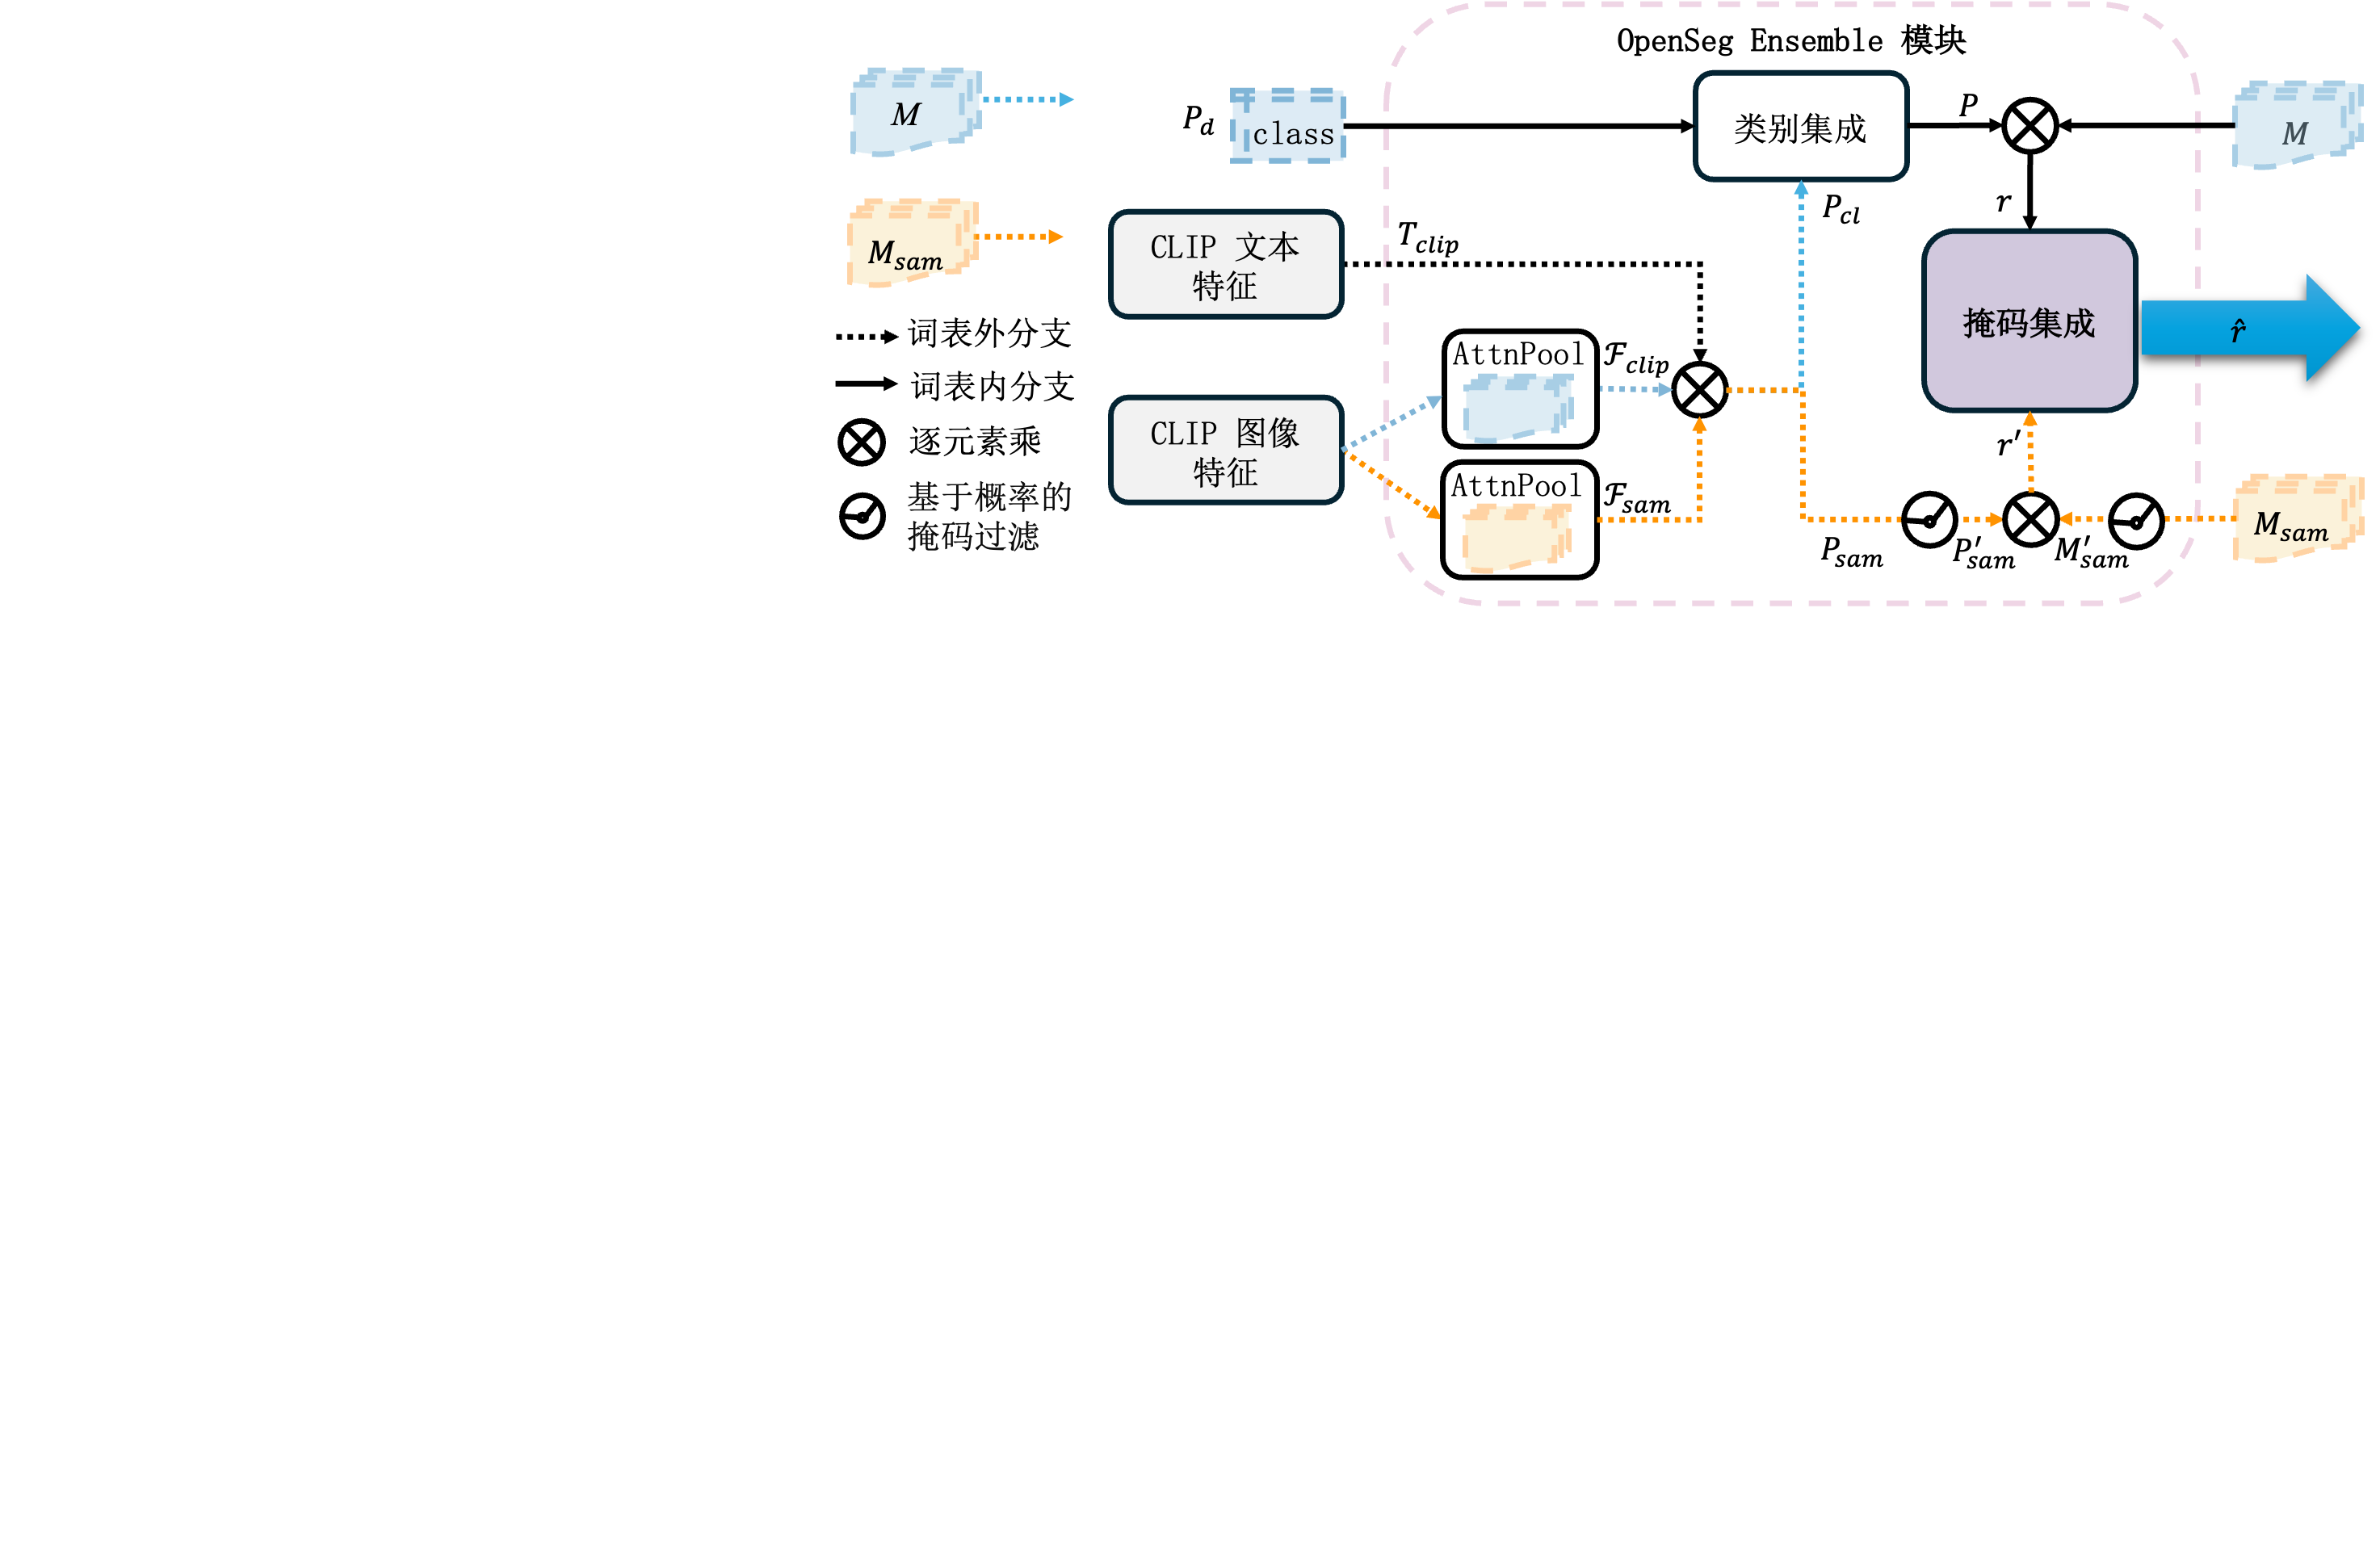
\includegraphics[width=0.95\textwidth]{figures/cmpf/maskEnsemble.png}
    \bicaption[fig:openseg_ensemble]{}{OpenSeg Ensemble模块结构示意图}{Fig.}{Architecture of the OpenSeg Ensemble Module}
\end{figure}


首先类别集成的目标是将检测器预测与CLIP直接预测进行有效融合。给定检测器预测$P_d=\{p_{i,d}\}_{i=1}^{N_q}$与基于掩码池化CLIP特征的CLIP预测$P_{\text{cl}}=\{p_{i,\text{cl}}\}_{i=1}^{N_q}$，类别集成通过加权几何平均计算融合后的类别概率：
\begin{equation}
p_i(j) = \begin{cases} (p_{i,d}(j))^{1-\alpha_{\text{ens}}} \cdot (p_{i,\text{cl}}(j))^{\alpha_{\text{ens}}}, & j \in \mathcal{C}_{\text{train}}, \\ (p_{i,d}(j))^{1-\beta_{\text{ens}}} \cdot (p_{i,\text{cl}}(j))^{\beta_{\text{ens}}}, & \text{otherwise}, \end{cases}
\label{eq:class_ensemble}
\end{equation}
其中$\alpha_{\text{ens}}=0.4$，$\beta_{\text{ens}}=0.8$为平衡系数。$P_{\text{cl}}$通过在掩码区域上对CLIP图像特征进行AttnPool池化后与文本特征对齐得到。
类别集成得到的概率-掩码对$(P, \mathcal{M})$被用于生成初步的语义分割结果$r = \sum_{i=1}^{N_q} p_i(c) \cdot m_{i,[x,y]}$。

掩码集成进一步引入SAM的零样本掩码预测。具体地，首先对$\mathcal{M}_{\text{sam}}$应用AttnPool得到SAM-CLIP特征并计算类别分数$P_{\text{sam}}$，使用阈值$\xi=0.5$过滤低质量掩码，得到选中的概率-掩码对$(\mathcal{M}'_{\text{sam}}, P'_{\text{sam}})$。

最终的语义分割结果$\hat{r}$通过两路预测的加权融合得到：
\begin{equation}
\hat{r}_{[x,y]}(j) = \begin{cases} r_{[x,y]}(j), & j \in \mathcal{C}_{\text{train}}, \\ (1-\epsilon_{\text{fuse}}) r_{[x,y]}(j) + \epsilon_{\text{fuse}} r'_{[x,y]}(j), & \text{otherwise}, \end{cases}
\label{eq:mask_ensemble}
\end{equation}
其中$\epsilon_{\text{fuse}}=0.2$控制SAM零样本掩码在未见类别上的融合权重。该设计使SAM的零样本分割能力专门用于提升未见类别的识别精度，而对训练集内的类别则保持原有检测器的预测，避免引入SAM的分割噪声。

在全景分割任务中，由于最终结果依赖单个查询的预测质量，集成更多含噪SAM掩码反而可能降低精度，因此仅采用类别集成而不进行掩码集成。

\section{实验结果与分析}

\subsection{数据集和实验设置}

模型仅在COCO Panoptic~\cite{lin2014microsoft}数据集上进行训练，该数据集包含133个类别。遵循零样本评估协议，模型在全景分割的ADE20K~\cite{zhou2017scene}、Cityscapes~\cite{cordts2016cityscapes}、BDD100K~\cite{yu2020bdd100k}三个基准上测试，使用PQ、AP、mIoU作为评价指标；在语义分割的PASCAL-Context（PC-459与PC-59）~\cite{mottaghi2014role}、ADE20K（A-847与A-150）两个基准上测试，使用mIoU作为评价指标；在实例分割的LVIS v1.0~\cite{gupta2019lvis}基准上测试，以rare类别的$\mathrm{AP}_r$作为主要评价指标。

实验采用RN50$\times$64与ConvNeXt-Large两种规模的CLIP图像编码器，以及ViT-Base的SAM图像编码器（基于消融分析的最优选择）。Transformer解码器层数$L_{\text{dec}}=9$，特征分辨率为$1/8$、$1/16$、$1/32$循环处理。Query Injector在第$3,6,9$层注入，Feature Injector在第$1,4,7$层应用。训练数据流为COCO Panoptic，4卡Tesla A100 GPU，batch size=16。推理时输入图像最短边resize到800像素（Cityscapes为1024），OpenSeg Ensemble默认参数$\alpha_{\text{ens}}=0.4$、$\beta_{\text{ens}}=0.8$、$\epsilon_{\text{fuse}}=0.2$，SAM使用ViT-Huge，$32\times 32$均匀采样点提示，独立生成类别无关的零样本掩码，并将其与解码器输出在未见类别上做加权融合。该阶段直接消费的是SAM输出的掩码质量本身，因此推理阶段改用规模更大的ViT-Huge。


\subsection{实验结果对比}

表~\ref{tab:panoptic_cmpf}给出了在ADE20K、Cityscapes与BDD100K三个数据集上的开放词汇全景分割结果。CMPF在所有数据集与骨干设置下均取得最优性能：在RN50$\times$64骨干下，全景分割指标较FC-CLIP有稳定的提升，在BDD100K上的差距相对更大。切换至ConvNeXt-L骨干后，三个数据集的全景分割指标进一步提升，说明跨模型先验融合策略的收益不依赖于特定骨干规模。
图~\ref{fig:cmpf_moti}与图~\ref{fig:cmpf_bdd}分别给出了Cityscapes与BDD100K上的全景分割可视化对比。可视化结果印证了定量分析：相较于FC-CLIP，CMPF在未见类别（如Cityscapes中的“rider”、BDD100K中的“vegetation”与“street light”）上展现出更强的泛化能力，同时对小目标的检测精度与独立实例的识别准确度也有明显改善。

\begin{table*}[!htbp]\centering
    \bicaption[tab:panoptic_cmpf]{}{开放词汇全景分割结果对比}{Table}{Open-vocabulary panoptic segmentation results}
    % \setlength{\tabcolsep}{1pt}
    \vspace{0.5em}\centering\wuhao
    % \resizebox{.8\textwidth}{!}{
    \begin{tabular}{lccccccccc}
        \toprule
        \multirow{2}{*}{方法} & \multirow{2}{*}{ViL Model} & \multicolumn{3}{c}{ADE20K} & \multicolumn{3}{c}{Cityscapes} & \multicolumn{2}{c}{BDD100K} \\
        \cline{3-10}
         &       & PQ & AP & mIoU & PQ & AP & mIoU & PQ & mIoU \\
        \midrule
        OPSNet~\cite{chen2023open}    & RN50        & 19.0 & --   & 25.4 & 41.5 & --   & --   & --   & --   \\
        MaskCLIP~\cite{ding2023open}  & ViT-L/14    & 15.1 & 6.0  & 23.7 & --   & --   & --   & --   & --   \\
        MasQCLIP~\cite{MasQCLIP} & ViT-L/14    & 23.3 & --   & 30.4 & --   & --   & --   & --   & --   \\
        ODISE~\cite{xu2023open}        & ViT-L/14    & 22.6 & 14.4 & 29.9 & --   & --   & --   & --   & --   \\
        ODISE+CLIPSelf~\cite{wu2024clipself} & ViT-L/14 & 23.7 & 13.6 & 30.1 & -- & -- & -- & -- & -- \\
        \midrule
        FC-CLIP~\cite{yu2023convolutions} & RN50$\times$64 & 21.3 & 13.2 & 28.7 & 42.6 & 27.3 & 55.1 & 13.8 & 41.4 \\
        \textbf{CMPF}                & RN50$\times$64 & \textbf{23.1} & \textbf{13.5} & \textbf{30.7} & \textbf{45.2} & \textbf{28.9} & \textbf{56.0} & \textbf{12.9} & \textbf{46.2} \\
        \midrule
        FC-CLIP~\cite{yu2023convolutions} & ConvNeXt-L & 25.1 & 16.4 & 32.8 & 44.3 & 27.9 & 56.0 & 17.9 & 49.4 \\
        EOV-Seg~\cite{niu2025eov}     & ConvNeXt-L  & 24.5 & 13.7 & 32.1 & --   & --   & --   & --   & --   \\
        \textbf{CMPF}                & ConvNeXt-L  & \textbf{25.9} & \textbf{16.5} & \textbf{34.4} & \textbf{45.8} & \textbf{28.4} & \textbf{56.8} & \textbf{19.3} & \textbf{52.3} \\
        \bottomrule
    \end{tabular}
    % }
\end{table*}


\begin{figure}[!htbp]
    \centering
    \subfigure[]{
    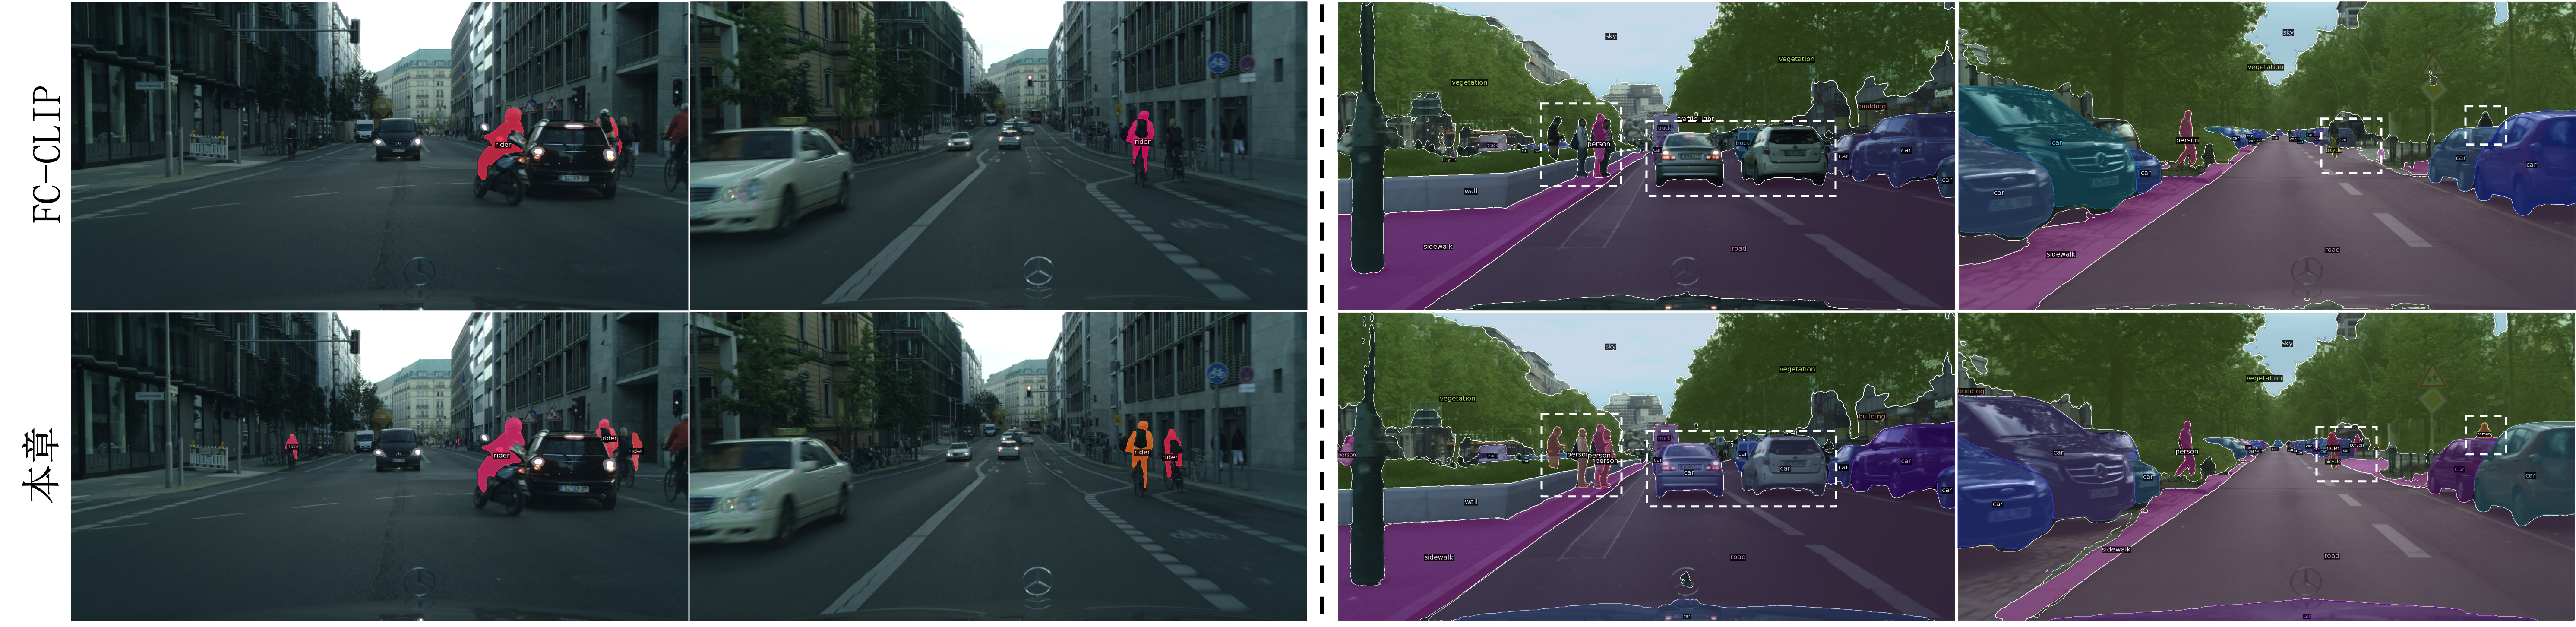
\includegraphics[width=1.\linewidth]{figures/cmpf/panop_city.png}
    \label{fig:cmpf_moti}
    }
    \subfigure[]{
    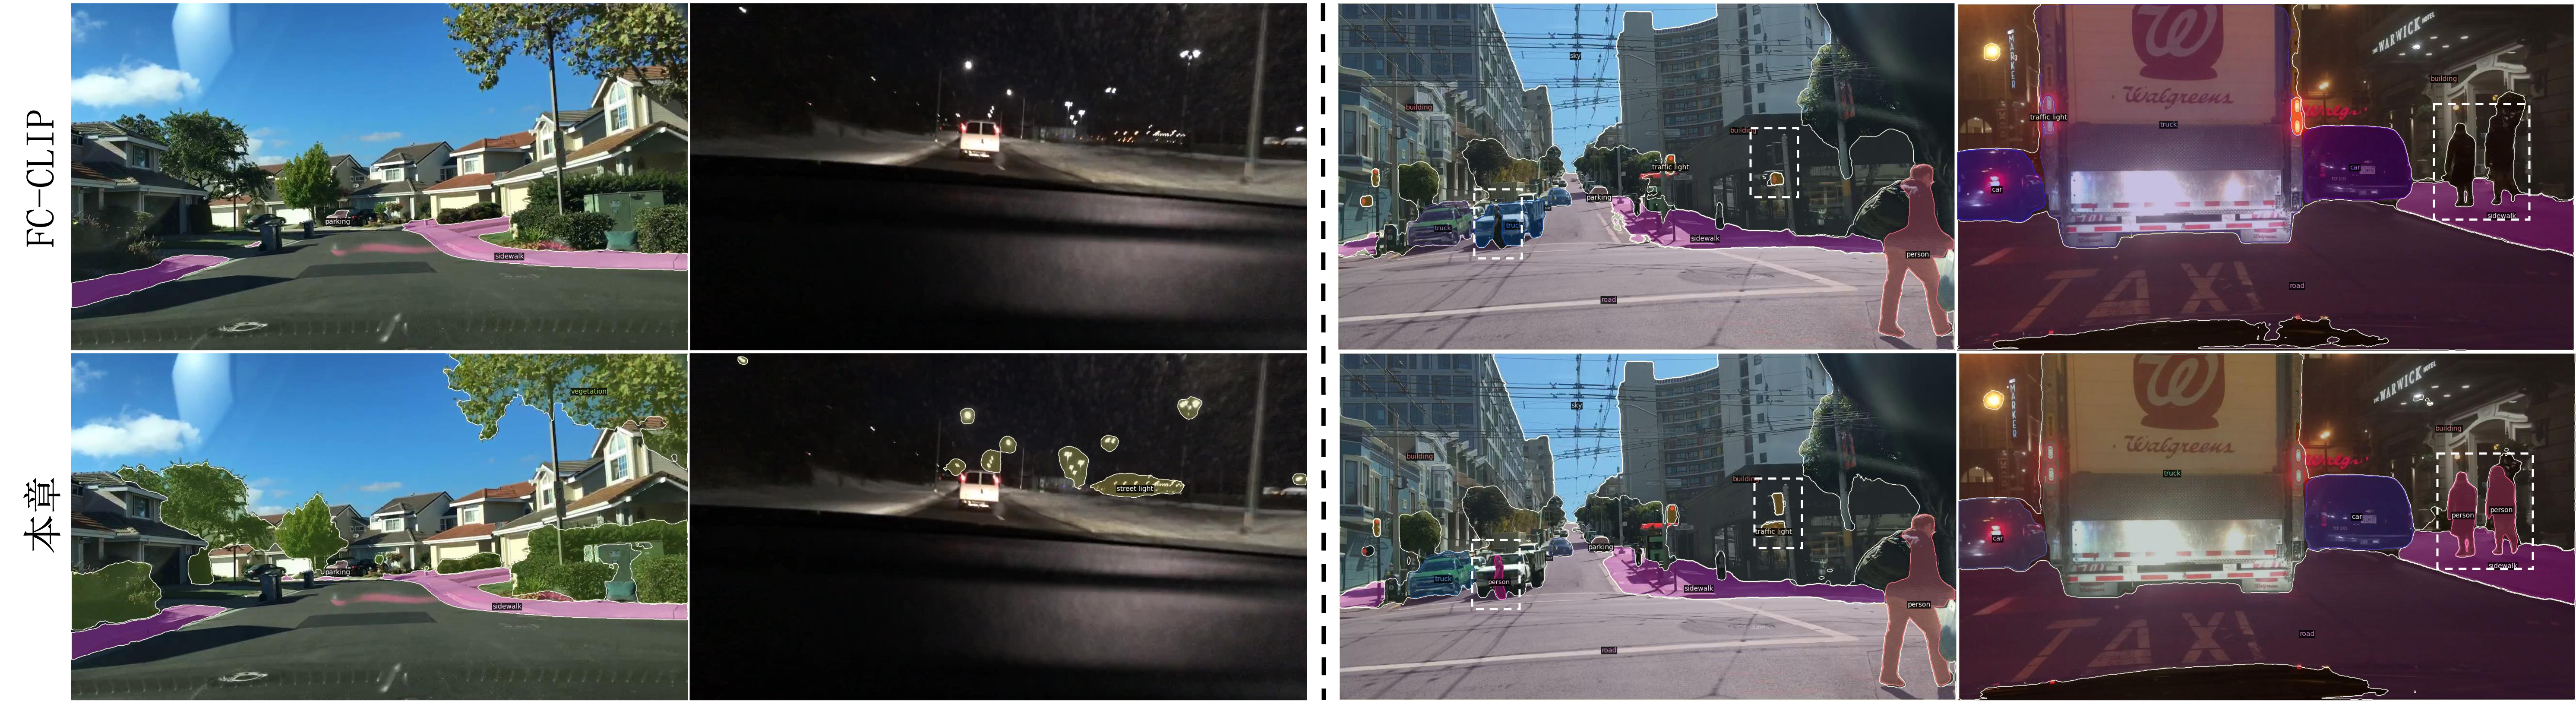
\includegraphics[width=1.\linewidth]{figures/cmpf/panop_bdd.png}
    \label{fig:cmpf_bdd}
    }
    \bicaption[fig:cmpf_city_bdd]{}{Cityscapes与BDD100K数据集上全景分割结果可视化对比}{Fig.}{Qualitative comparison of panoptic segmentation results on Cityscapes and BDD100K}
\end{figure}


表~\ref{tab:semantic_cmpf}给出了四个语义分割基准上的结果。CMPF在所有数据集上均刷新了最优性能，无论采用RN50$\times$64还是ConvNeXt-L骨干均取得明显提升；值得注意的是，CMPF仅使用COCO Panoptic的133个类别训练，而同期方法SCAN~\cite{liu2024open}使用COCO Stuff的171个类别训练且仅支持语义分割，CMPF在更少训练类别与更广任务覆盖下仍实现了更优性能，体现了该方法在数据效率与泛化能力上的双重优势。如图~\ref{fig:cmpf_pc459}与图~\ref{fig:cmpf_a847}所示，相较于MaskCLIP与FC-CLIP，CMPF在保持结构完整性与上下文一致性方面表现更优，尤其在未见类别的分割边界上展现出更强的泛化能力，可视化结果与定量数据高度一致。

\begin{table*}[!htbp]\centering
    \bicaption[tab:semantic_cmpf]{}{开放词汇语义分割结果对比}{Table}{Open-vocabulary semantic segmentation results}
    % \setlength{\tabcolsep}{2pt}
    \vspace{0.5em}\centering\wuhao
    % \resizebox{.6\textwidth}{!}{
    \begin{tabular}{llcccc}
        \toprule
        方法 & ViL Model & PC-459 & PC-59 & A-847 & A-150 \\
        \midrule
        ZegFormer~\cite{ding2022decoupling}    & ViT-B/16   & --    & --    & --    & 16.4 \\
        SimBase~\cite{xu2022simple}            & ViT-B/16   & --    & 47.7  & 7.0   & 20.5 \\
        OpenSeg~\cite{ghiasi2022scaling}       & ALIGN      & 11.2  & 45.9  & 6.8   & 24.8 \\
        OPSNet~\cite{chen2023open}             & RN50       & --    & 54.3  & --    & 25.4 \\
        \midrule
        Ovseg~\cite{liang2023open}             & ViT-L/14   & 12.4  & 55.7  & 9.0   & 29.6 \\
        MaskCLIP~\cite{ding2023open}           & ViT-L/14   & 10.0  & 45.9  & 8.2   & 23.7 \\
        MasQCLIP~\cite{MasQCLIP}         & ViT-L/14   & 18.2  & 57.8  & 10.7  & 30.4 \\
        ODISE~\cite{xu2023open}                & ViT-L/14   & 14.5  & 57.3  & 11.1  & 29.9 \\
        SCAN~\cite{liu2024open}                & ViT-L/14   & 16.7  & 59.3  & 14.0  & 33.5 \\
        \midrule
        FC-CLIP~\cite{yu2023convolutions}      & RN50$\times$64 & 15.6 & 54.8 & 10.8 & 28.7 \\
        \textbf{CMPF}                          & RN50$\times$64 & \textbf{18.7} & \textbf{57.5} & \textbf{11.8} & \textbf{30.7} \\
        \midrule
        FC-CLIP~\cite{yu2023convolutions}      & ConvNeXt-L & 17.3  & 56.6  & 14.0  & 32.8 \\
        EOV-Seg~\cite{niu2025eov}              & ConvNeXt-L & 16.8  & 56.9  & 12.8  & 32.1 \\
        \textbf{CMPF}                          & ConvNeXt-L & \textbf{19.7} & \textbf{58.4} & \textbf{14.8} & \textbf{34.4} \\
        \bottomrule
    \end{tabular}
    % }
\end{table*}


\begin{figure}[!htbp]
    \centering
    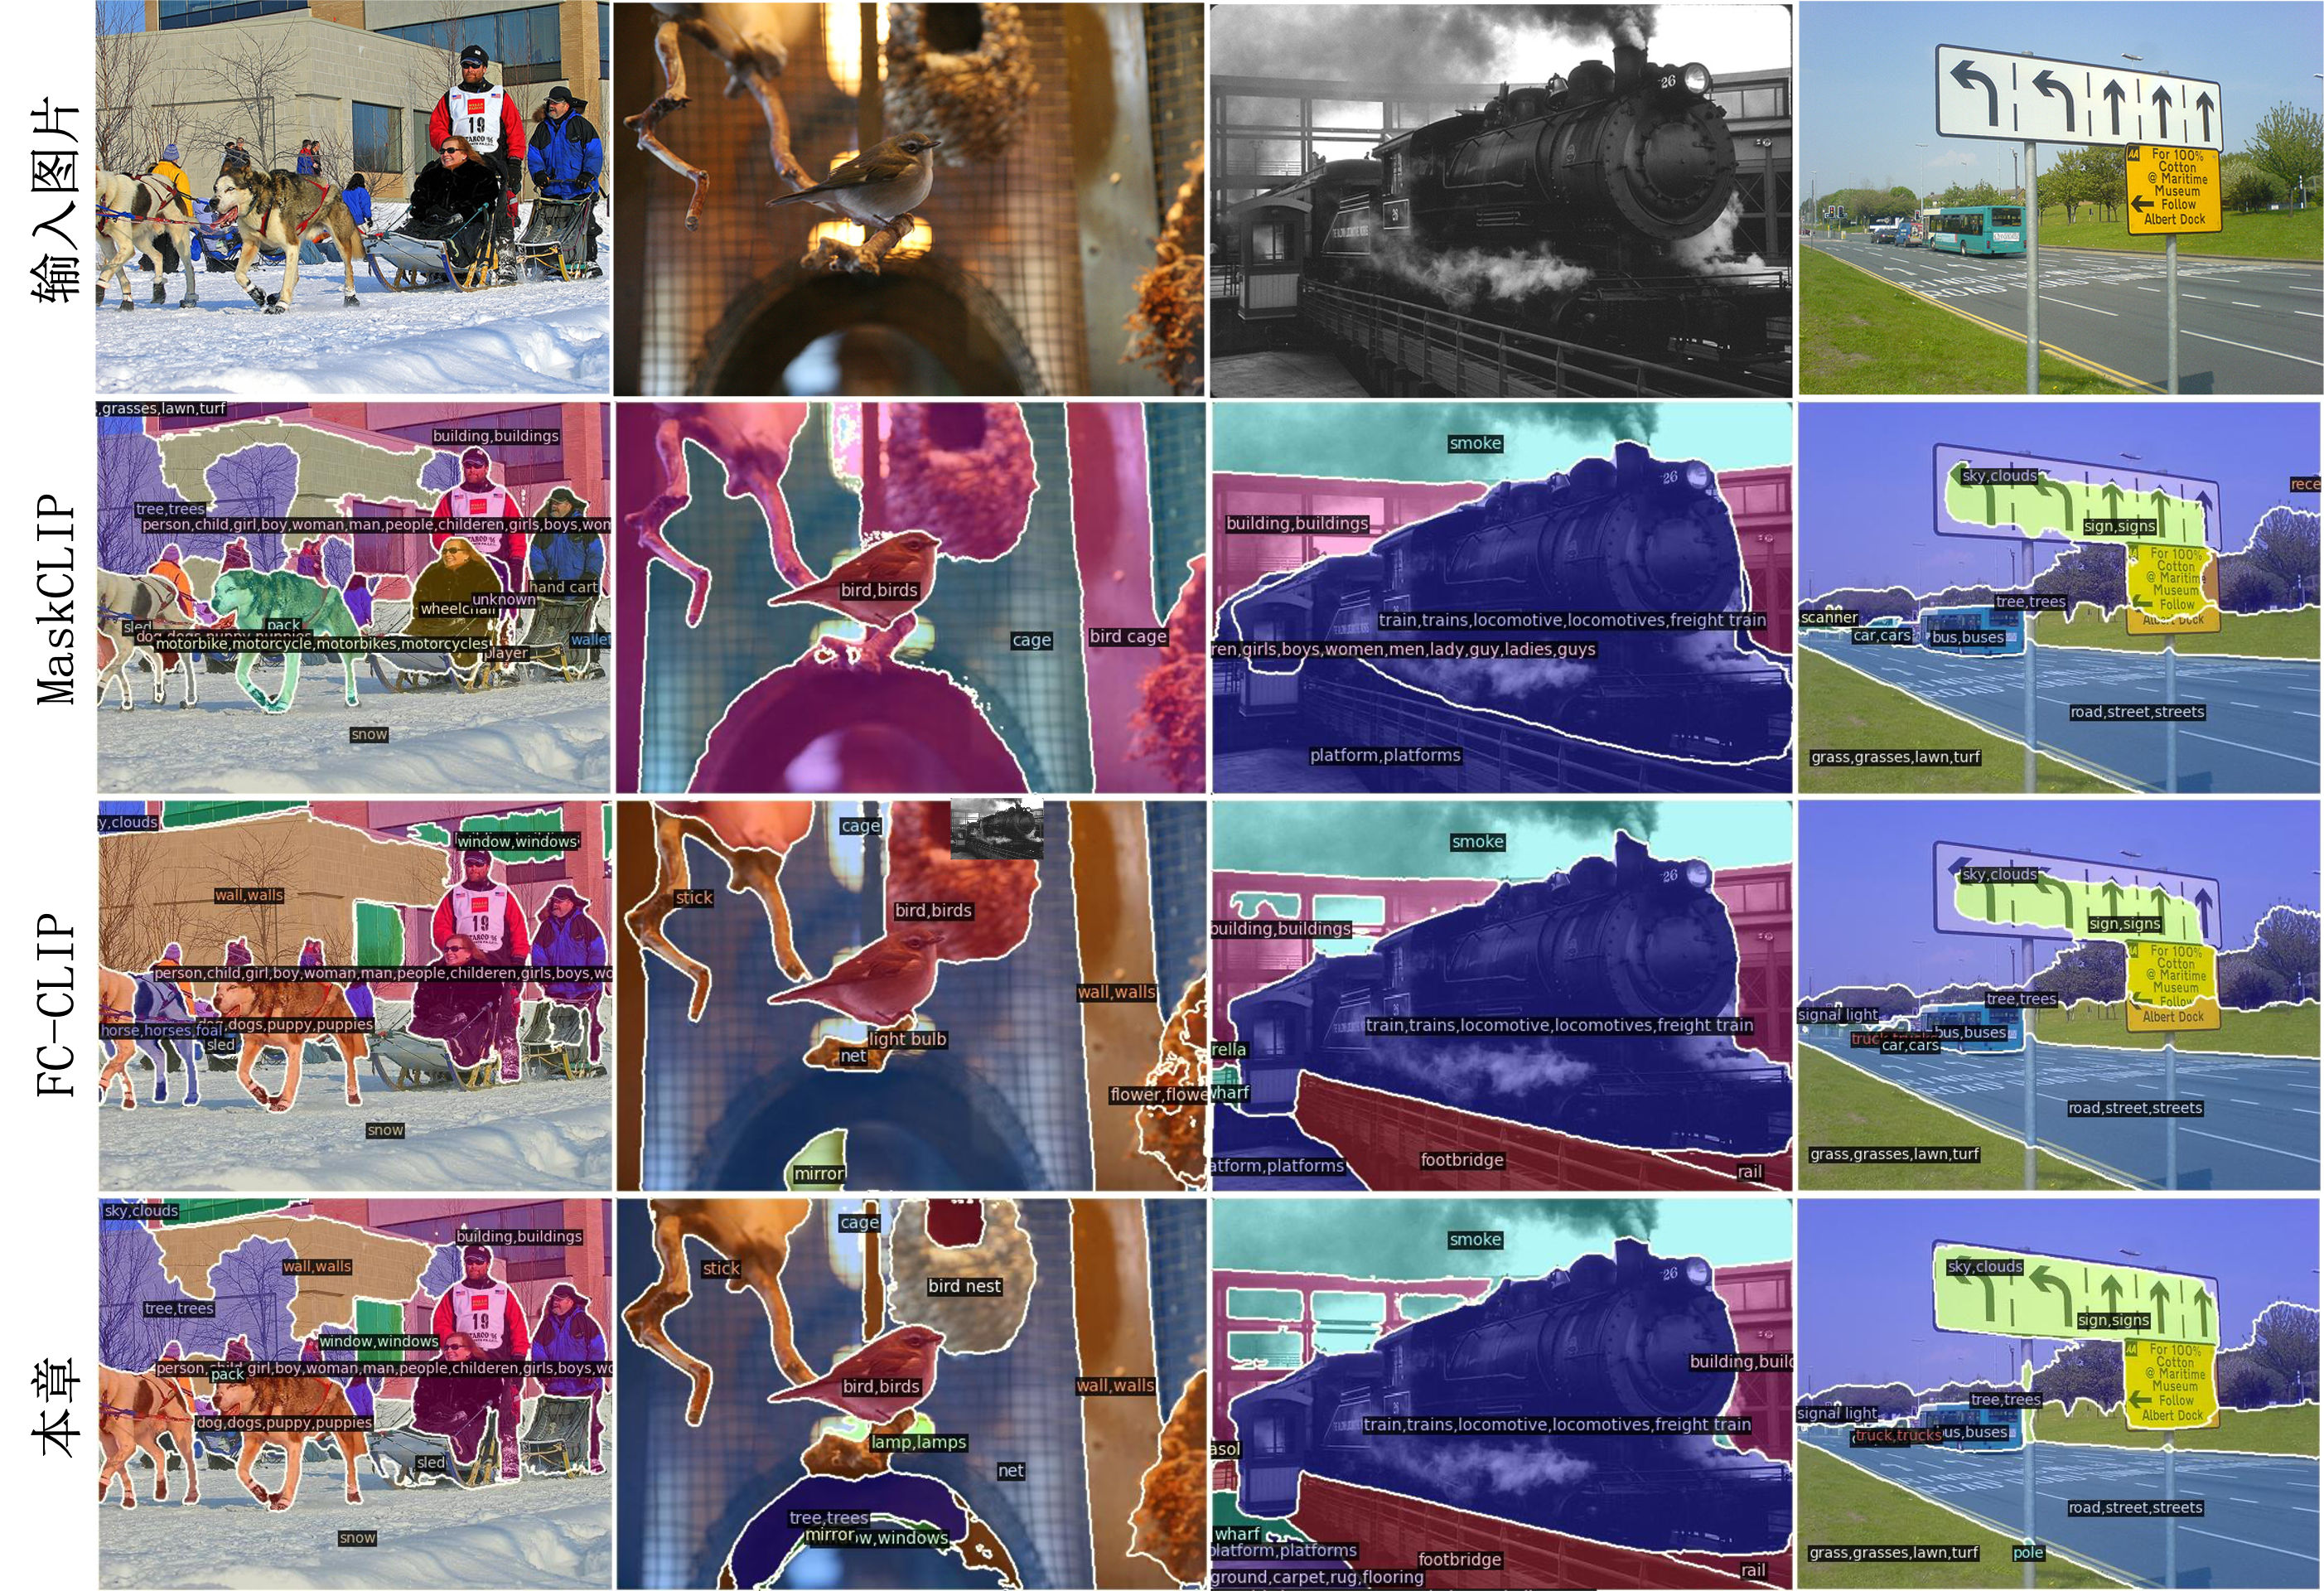
\includegraphics[width=0.95\textwidth]{figures/cmpf/sem_pc459.png}
    \bicaption[fig:cmpf_pc459]{}{PC-459数据集上语义分割结果可视化对比}{Fig.}{Qualitative comparison of semantic segmentation on PC-459}
\end{figure}

\begin{figure}[!htbp]
    \centering
    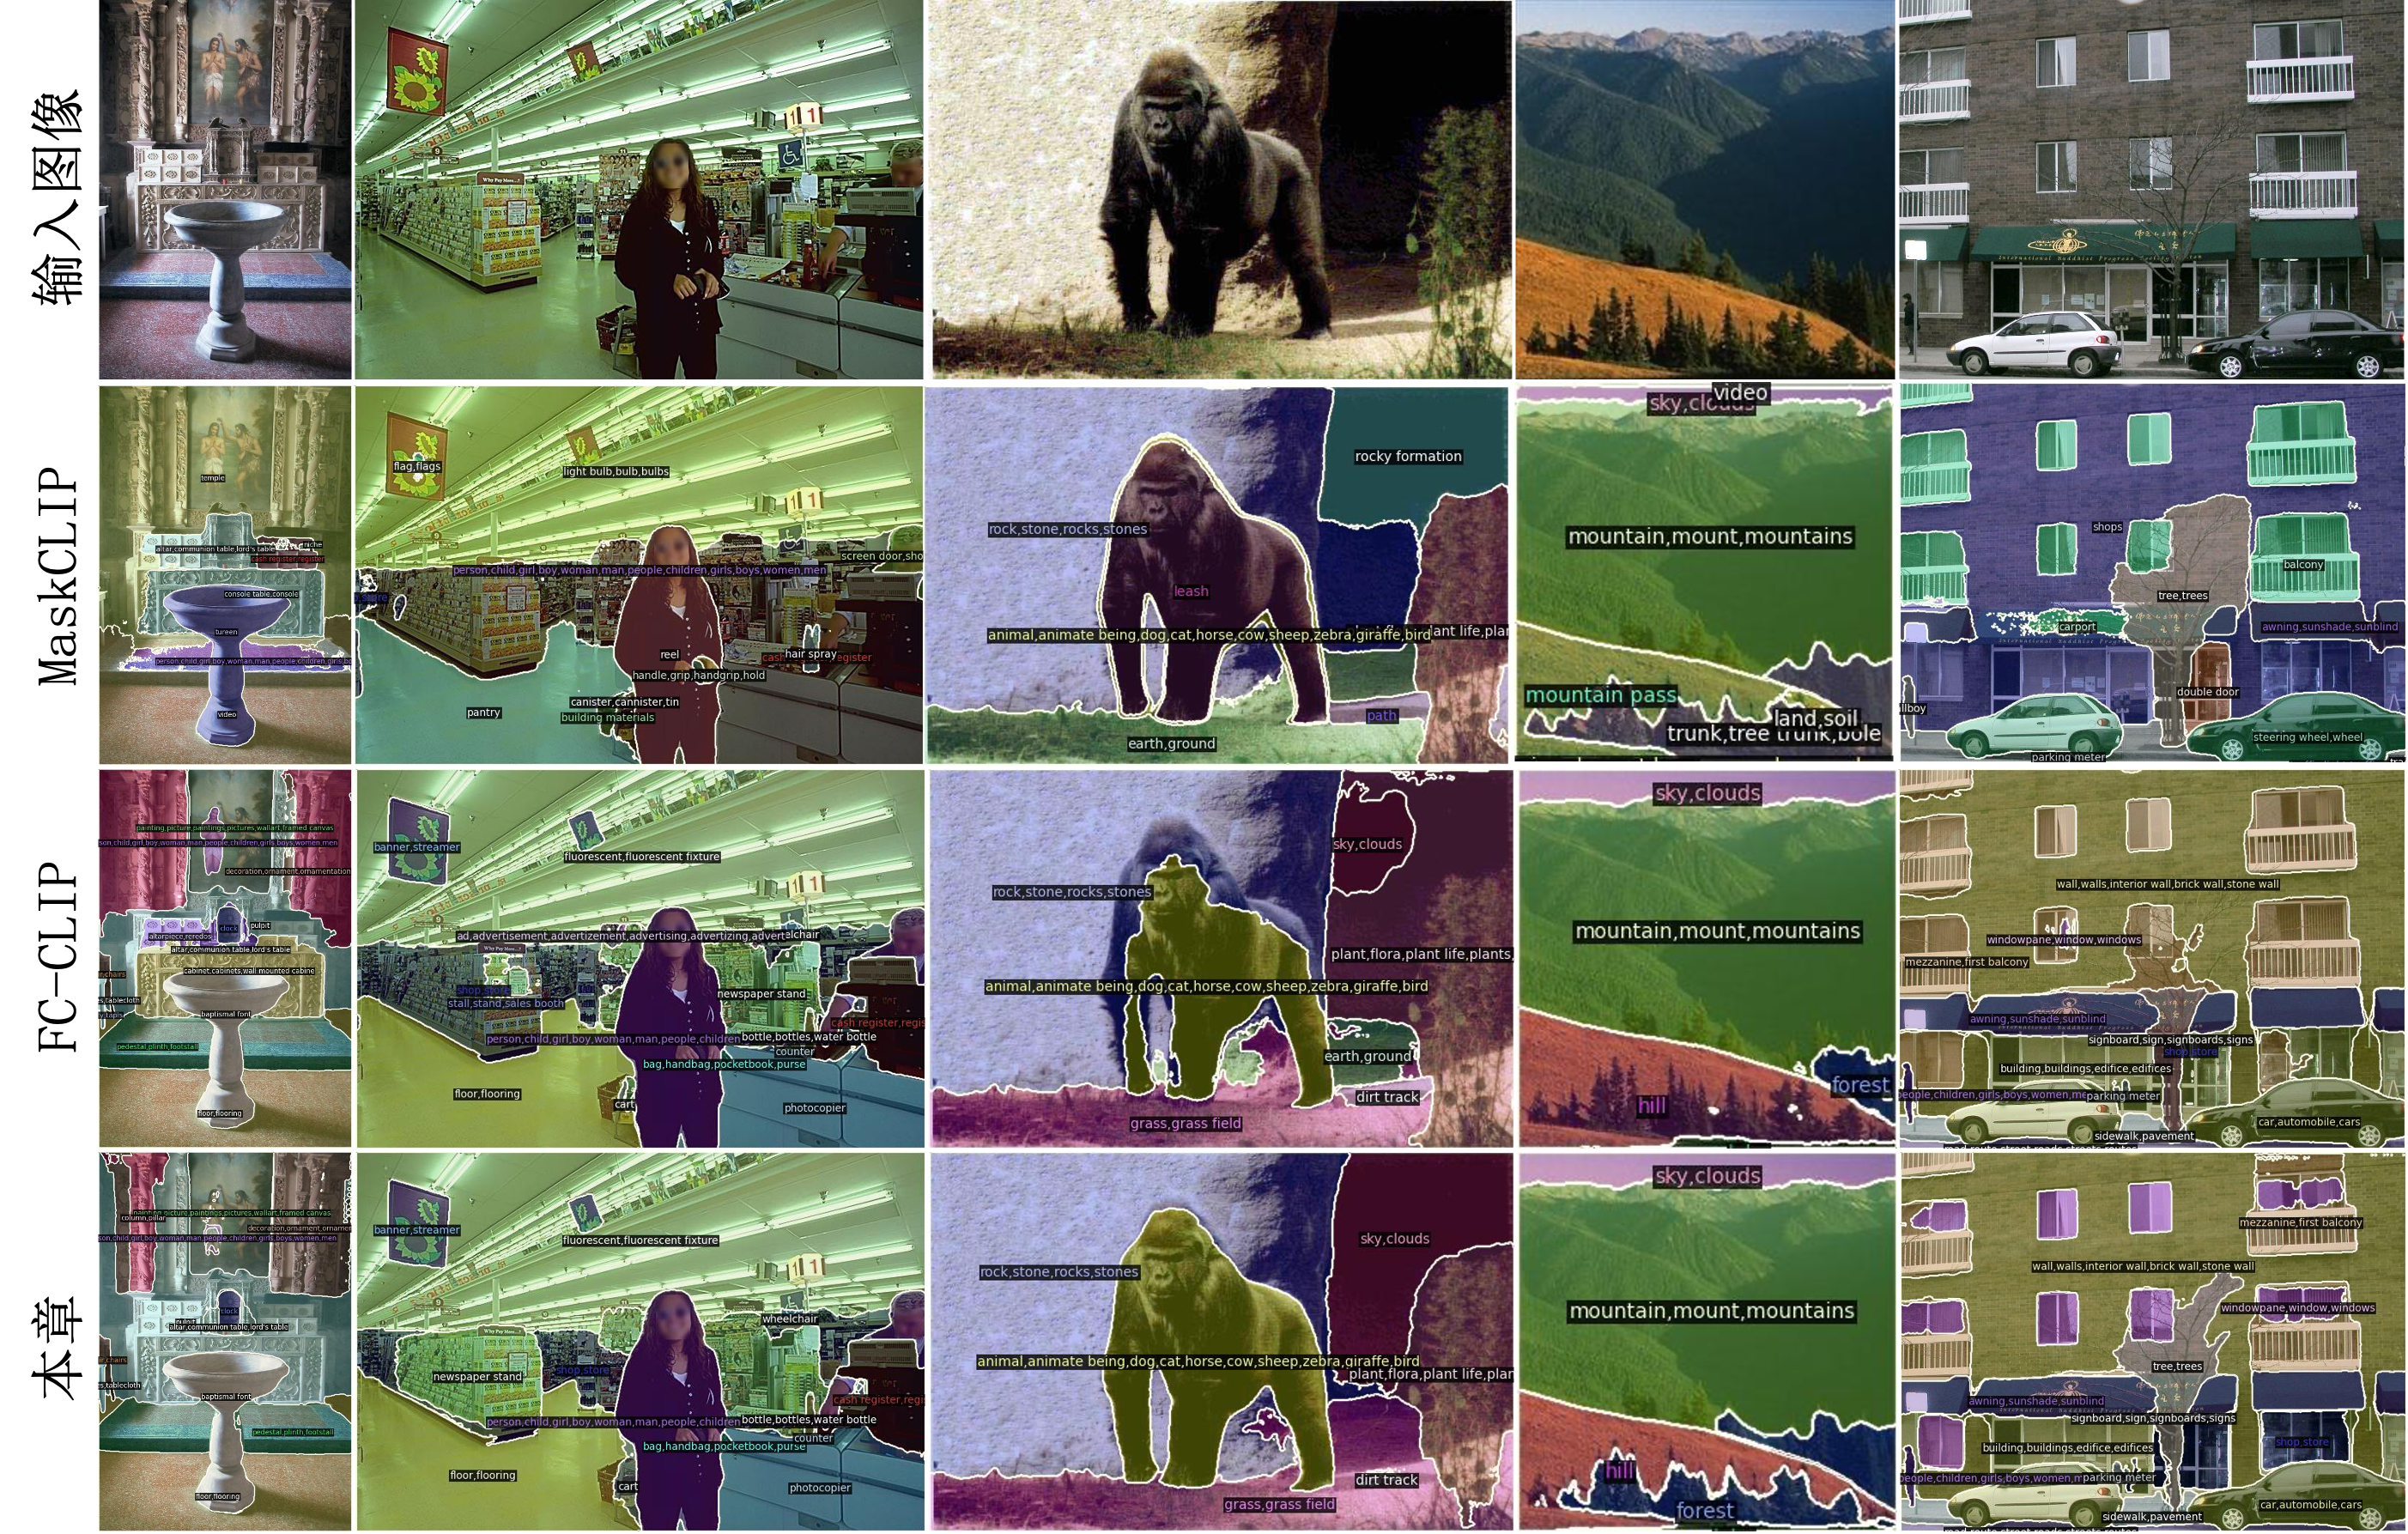
\includegraphics[width=0.95\textwidth]{figures/cmpf/sem_a847.png}
    \bicaption[fig:cmpf_a847]{}{A-847数据集上语义分割结果可视化对比}{Fig.}{Qualitative comparison of semantic segmentation on A-847}
\end{figure}

表~\ref{tab:instance_cmpf}给出了在LVIS v1.0数据集rare类别上的实例分割结果，CMPF（ConvNeXt-L）在该指标上高于RegionSpot~\cite{yang2024recognize}与Open-Vocabulary SAM~\cite{yuan2024open}等依赖额外box proposals与大规模外部数据集的方法。需要注意的是，两类对比方法的训练条件与本章方法并不相同：前者分别引入了额外的预检测器与更大规模的外部训练数据，因此该表所能支持的结论限于本章方法在更受限的训练条件下取得了当前最优的rare类别精度，而非方法本身的绝对优势；本章方法以端到端方式生成proposals，仅依赖COCO Panoptic训练，无需额外的预检测器或外部数据。


\begin{table*}[!htbp]\centering
    \bicaption[tab:instance_cmpf]{}{LVIS v1.0数据集rare类别开放词汇实例分割结果对比}{Table}{Open-vocabulary instance segmentation on LVIS rare}
    \setlength{\tabcolsep}{2pt}
    \vspace{0.5em}\centering\wuhao
    % \resizebox{.8\textwidth}{!}{%
    \begin{tabular}{lcccc}
        \toprule
        方法 & ViL Model & 训练数据 & 外部提议 & $\text{AP}_r$ \\
        \midrule
        & ViT-B/16 & O365 & GLIP-T(B) & 12.7 \\
        RegionSpot~\cite{yang2024recognize} & ViT-L/14 & O365, OI, V3D & SAM-B & 14.3 \\
        & ViT-B/16 & O365, OI, V3D & GLIP-T & 20.0 \\
        \midrule
        Open-Vocabulary SAM~\cite{yuan2024open} & RN50$\times$16 & SAM-1B+LVIS$^\ddag$ & Detic & 24.0 \\
        \midrule
        FC-CLIP~\cite{yu2023convolutions} & ConvNeXt-L & COCO Panoptic & -- & 25.0 \\
        \textbf{CMPF} & ConvNeXt-L & COCO Panoptic & -- & \textbf{25.6} \\
        \bottomrule
    \end{tabular}
    % }
\end{table*}


\begin{figure}[!htbp]
    \centering
    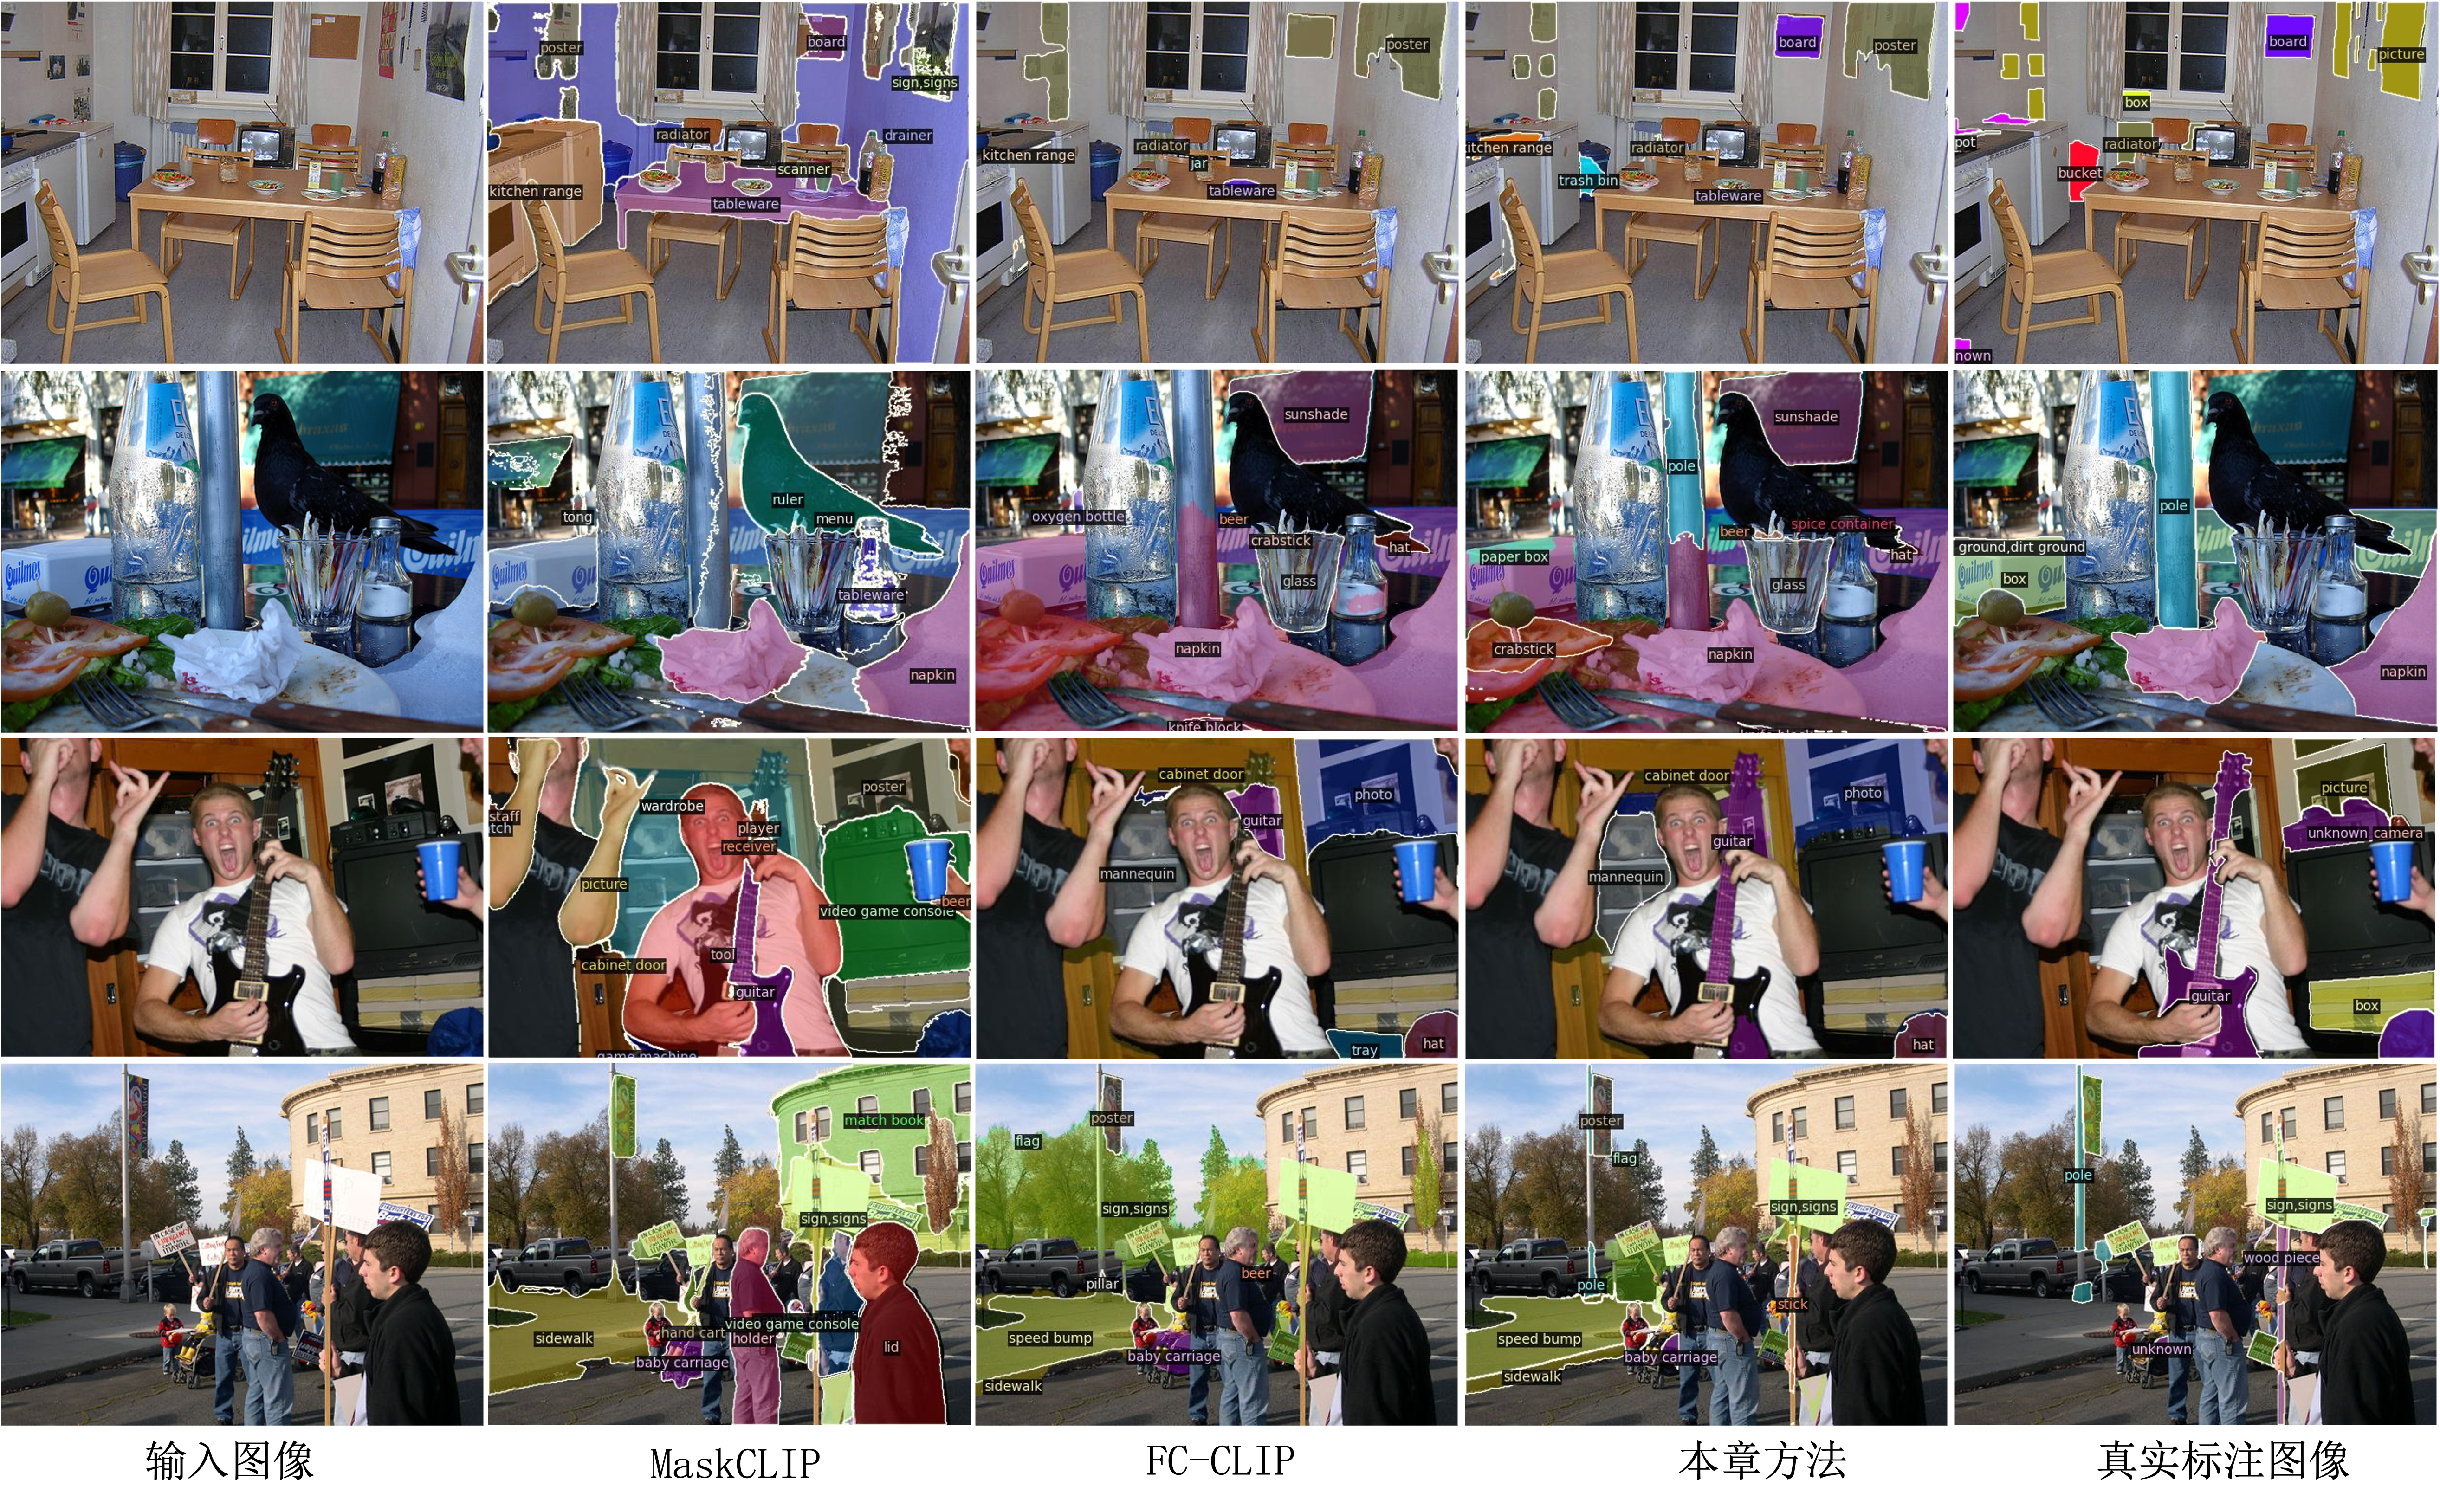
\includegraphics[width=0.95\textwidth]{figures/cmpf/Com_unseen.png}
    \bicaption[fig:cmpf_unseen]{}{PC-459数据集上未见类别零样本语义分割结果可视化}{Fig.}{Zero-shot semantic segmentation on unseen classes of PC-459}
\end{figure}

\begin{table*}[!htbp]\centering
    \bicaption[tab:unseen_cmpf]{}{开放词汇语义分割可见/未见类别mIoU对比（\%）}{Table}{mIoU on seen/unseen classes}
    \vspace{0.5em}\centering\wuhao
    \setlength{\tabcolsep}{2pt}
    \resizebox{.8\textwidth}{!}{%
    \begin{tabular}{lcccccc}
        \toprule
        \multirow{2}{*}{方法} & \multicolumn{2}{c}{PC-459} & \multicolumn{2}{c}{A-847} & \multicolumn{2}{c}{A-150} \\
        \cline{2-7}
         & $\text{mIoU}_{seen}$ & $\text{mIoU}_{unseen}$ & $\text{mIoU}_{seen}$ & $\text{mIoU}_{unseen}$ & $\text{mIoU}_{seen}$ & $\text{mIoU}_{unseen}$ \\
        \midrule
        MaskCLIP~\cite{ding2023open}  & 30.3 & 6.3 & 16.7 & 6.0 & 32.7 & 16.5 \\
        FC-CLIP~\cite{yu2023convolutions} & 46.0 & 8.7 & 34.0 & 11.3 & 47.3 & 22.0 \\
        \textbf{CMPF}                & \textbf{48.1} & \textbf{11.2} & \textbf{34.7} & \textbf{12.1} & \textbf{49.0} & \textbf{23.6} \\
        \bottomrule
    \end{tabular}}
\end{table*}


围绕未见类别这一开放词汇分割的核心场景，本节从可视化与定量两方面展开分析。PC-459数据集上“poster”、“board”、“pole”等未见类别的零样本语义分割效果优于对比方法（如图~\ref{fig:cmpf_unseen}所示），定性印证了Query Injector对掩码生成质量的提升；表~\ref{tab:unseen_cmpf}进一步从定量角度对比了CMPF在可见与未见类别上的分割表现，未见类别上取得提升的同时，可见类别上也保持竞争力，表明SAM空间先验的融合不仅强化了开放词汇泛化能力，也未损害对训练类别的判别精度。

表~\ref{tab:recall_cmpf}从掩码质量角度报告了不同IoU阈值（0.5/0.75/0.9）下的召回率，CMPF在所有阈值上均显著优于FC-CLIP在未见类别上的掩码提议，验证了Query Injector对掩码生成质量的系统性提升。

\begin{table*}[!htbp]
    \bicaption[tab:recall_cmpf]{}{开放词汇语义分割掩码召回率}{Table}{Open-vocabulary semantic mask recall }
    \vspace{0.5em}\centering\wuhao
    \setlength{\tabcolsep}{1pt}
    \resizebox{\textwidth}{!}{
    \begin{tabular}{lccccccccc}
        \toprule
        \multirow{2}{*}{方法} & \multicolumn{3}{c}{PC-459 (S/U)} & \multicolumn{3}{c}{A-847 (S/U)} & \multicolumn{3}{c}{A-150 (S/U)} \\
        \cline{2-10}
         & 0.5 & 0.75 & 0.9 & 0.5 & 0.75 & 0.9 & 0.5 & 0.75 & 0.9 \\
        \midrule
        FC-CLIP & 91.4/77.7 & 73.6/56.2 & 43.9/28.4 & \textbf{84.6}/66.6 & \textbf{60.0}/41.3 & \textbf{27.6}/14.3 & 83.7/72.0 & 58.9/45.5 & \textbf{27.7}/17.4 \\
        \textbf{CMPF} & \textbf{92.6/81.0} & \textbf{76.0/59.9} & \textbf{47.0/31.4} & 78.9/\textbf{82.9} & 52.3/\textbf{59.4} & 23.6/\textbf{24.6} & \textbf{84.7}/\textbf{73.2} & \textbf{60.1}/\textbf{47.2} & 27.6/\textbf{18.0} \\
        \bottomrule
    \end{tabular}}
\end{table*}


\FloatBarrier
\subsection{消融实验}

\noindent\textbf{（1）多尺度双注入器和零样本掩码集成有效性}

表~\ref{tab:ablation_cmpf}给出了CMPF三个核心组件的消融结果。单独使用SAM的proposals（Model 1）时，三个数据集上的性能说明SAM具有基础泛化能力但缺乏语义指导。在统一框架下逐步加入三个模块，指标持续提升：Query Injector引入细粒度空间查询后性能大幅改善，Feature Injector进一步精炼了语义—空间特征融合，OpenSeg Ensemble在推理阶段提供了互补增益。值得注意的是，仅依靠OpenSeg Ensemble的提升有限，说明SAM空间信息的深度融合——即两个Injector——是性能提升的主要驱动力。

\begin{table}[!htbp]\centering
    \bicaption[tab:ablation_cmpf]{}{CMPF各模块消融结果}{Table}{Ablation of CMPF components}
    \vspace{0.5em}\centering\wuhao
    \setlength{\tabcolsep}{2pt}
    \begin{tabular}{cccccccc}
        \toprule
        &\multirow{2}{*}{Query Injector} & \multirow{2}{*}{Feature Injector} & \multirow{2}{*}{OpenSeg Ensemble} & \multicolumn{3}{c}{Semantic} & Panoptic \\
        \cline{5-8}
        & &       &       & PC-459 & A-847 & A-150 & A-150 (PQ) \\
        \midrule
        Model 1&$\times$ & $\times$ & $\times$ & 17.3 & 14.0 & 32.8 & 25.1 \\
        Model 2&$\times$ & $\times$ & \checkmark & 17.6 & 14.5 & 33.5 & -- \\
        Model 3&$\checkmark$ & $\times$ & $\times$ & 18.1 & 14.2 & 33.6 & 25.7 \\
        Model 4&$\checkmark$ & $\checkmark$ & $\times$ & 18.5 & 14.4 & 33.8 & 25.9 \\
        CMPF   & $\checkmark$& $\checkmark$ & $\checkmark$ & \textbf{19.7} & \textbf{14.8} & \textbf{34.4} & -- \\
        \bottomrule
    \end{tabular}
\end{table}


图~\ref{fig:abl_atten}给出了不同消融设置下的实例级注意力图对比。单独使用CLIP时，模型对未见类别的激活区域有限；引入Query Injector后，模型能够激活先前未识别的物体区域，尤其对未见类别效果显著；Feature Injector则进一步精炼了注意力的空间分布，使激活模式更加完整和一致。两个Injector在增强物体定位与空间一致性方面发挥着互补的协同作用。

\begin{figure}[!htbp]
    \centering
    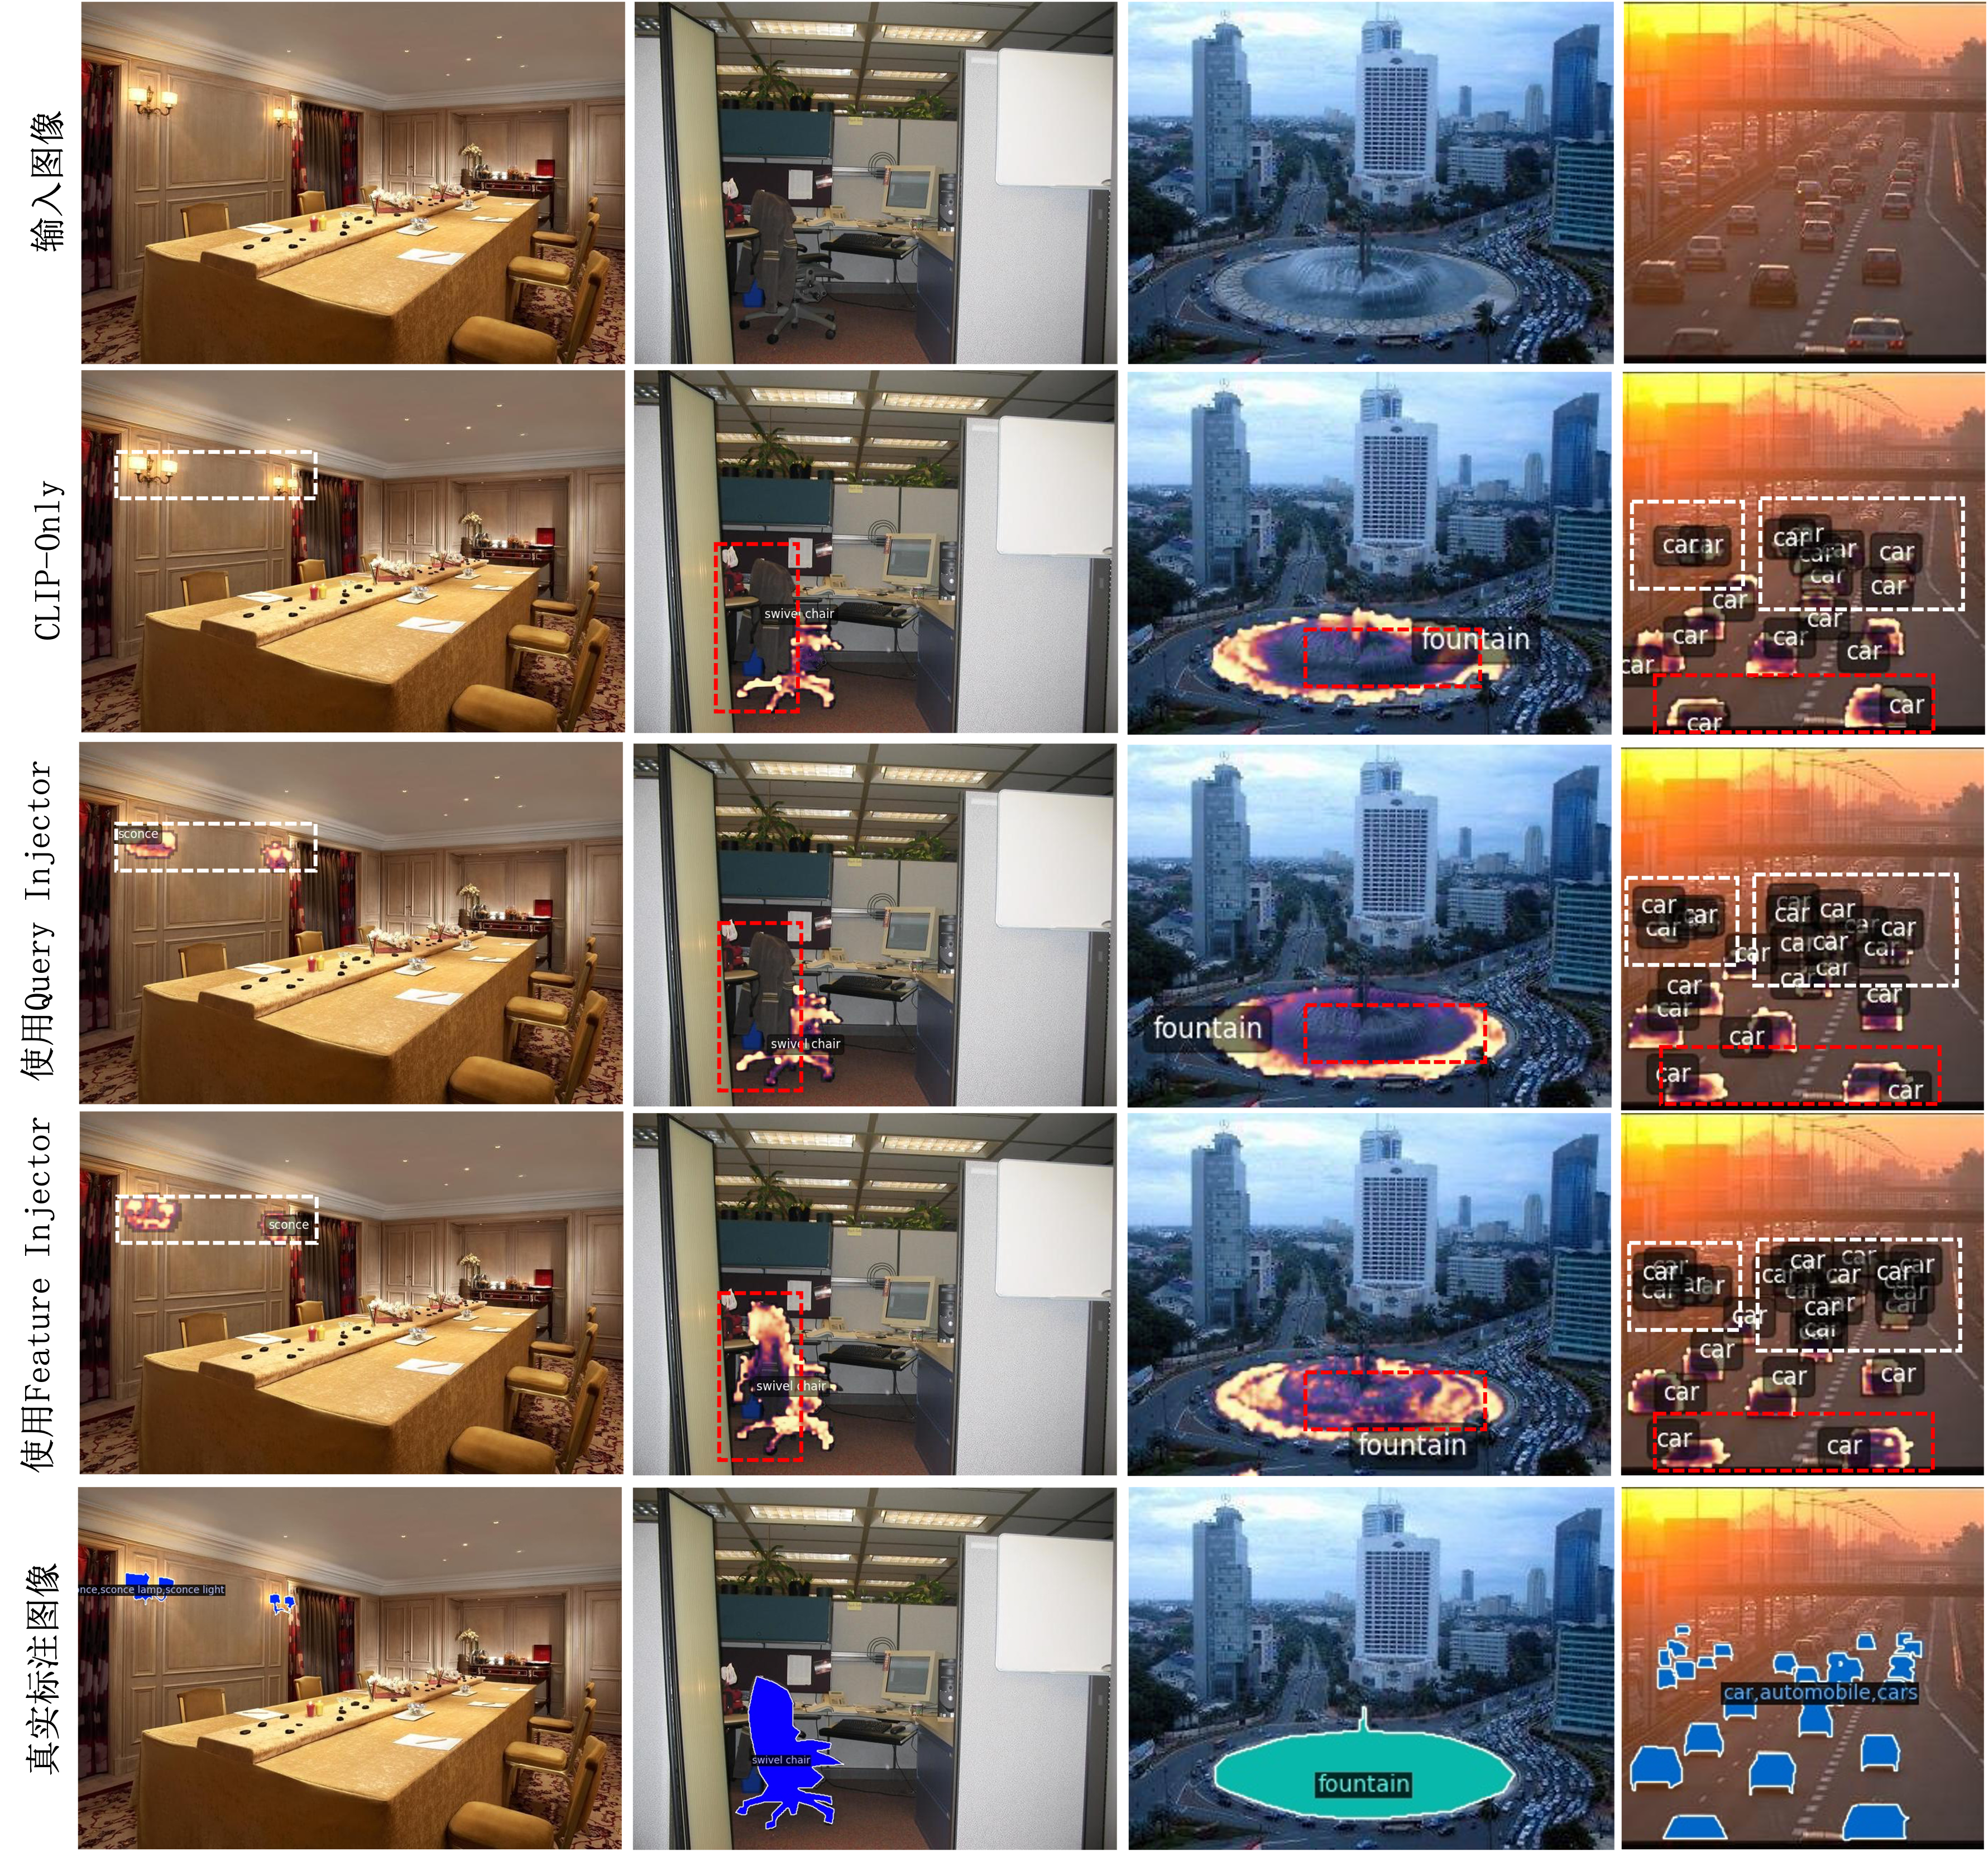
\includegraphics[width=0.95\textwidth]{figures/cmpf/abl_atten2.png}
    \bicaption[fig:abl_atten]{}{ADE20K数据集上实例级注意力图消融对比}{Fig.}{Instance-level attention map ablation comparison on ADE20K}
\end{figure}


\noindent\textbf{（2）SAM对掩码质量优化的影响}

表~\ref{tab:sam_cmpf} 对比了不同规模 SAM 骨干对 CMPF 性能的影响，该结果同时是训练阶段选型依据的来源。ViT-B 规模在所有数据集上均取得最佳或近最佳性能：其 Cityscapes 全景分割 PQ 达到 45.8\%，高于 ViT-L 与 ViT-H 的 44.2\%；语义分割上 PC-459 取得 18.5\%，亦优于其他三种配置。这一结果与前述设计依据相互印证——训练阶段需要的是实例可分性而非边界精细度，ViT-T 提供的边界较粗、实例连通性不足，ViT-L/ViT-H 虽然单点精度更高，但实例连通性有所下降，对全景分割的整体质量构成不利影响。ViT-B 规模因此在分割精度与实例连通性之间取得平衡，被确定为训练阶段的编码器配置。

\begin{table}[!htbp]\centering
    \bicaption[tab:sam_cmpf]{}{不同SAM骨干规模对CMPF性能的影响}{Table}{Effect of SAM backbone size}
    \vspace{0.5em}\centering\wuhao
    % \setlength{\tabcolsep}{2pt}
    % \resizebox{.5\textwidth}{!}{
    \begin{tabular}{lcccccc}
        \toprule
        \multirow{2}{*}{SAM} & \multicolumn{3}{c}{Cityscapes} & \multicolumn{3}{c}{Semantic} \\
        \cline{2-7}
         & PQ & AP & mIoU & PC-459 & A-847 & PC-59 \\
        \midrule
        ViT-T & 43.0 & 25.9 & 55.0 & 17.6 & 14.0 & 56.8 \\
        \textbf{ViT-B} & \textbf{45.8} & \textbf{28.4} & \textbf{56.8} & \textbf{18.5} & \textbf{14.4} & \textbf{58.1} \\
        ViT-L & 44.2 & 27.1 & 56.2 & 17.4 & 14.2 & 56.7 \\
        ViT-H & 44.2 & 28.0 & 56.2 & 17.3 & 13.9 & 56.6 \\
        \bottomrule
\end{tabular}
% }
\end{table}


\begin{figure}[!htbp]
    \centering
    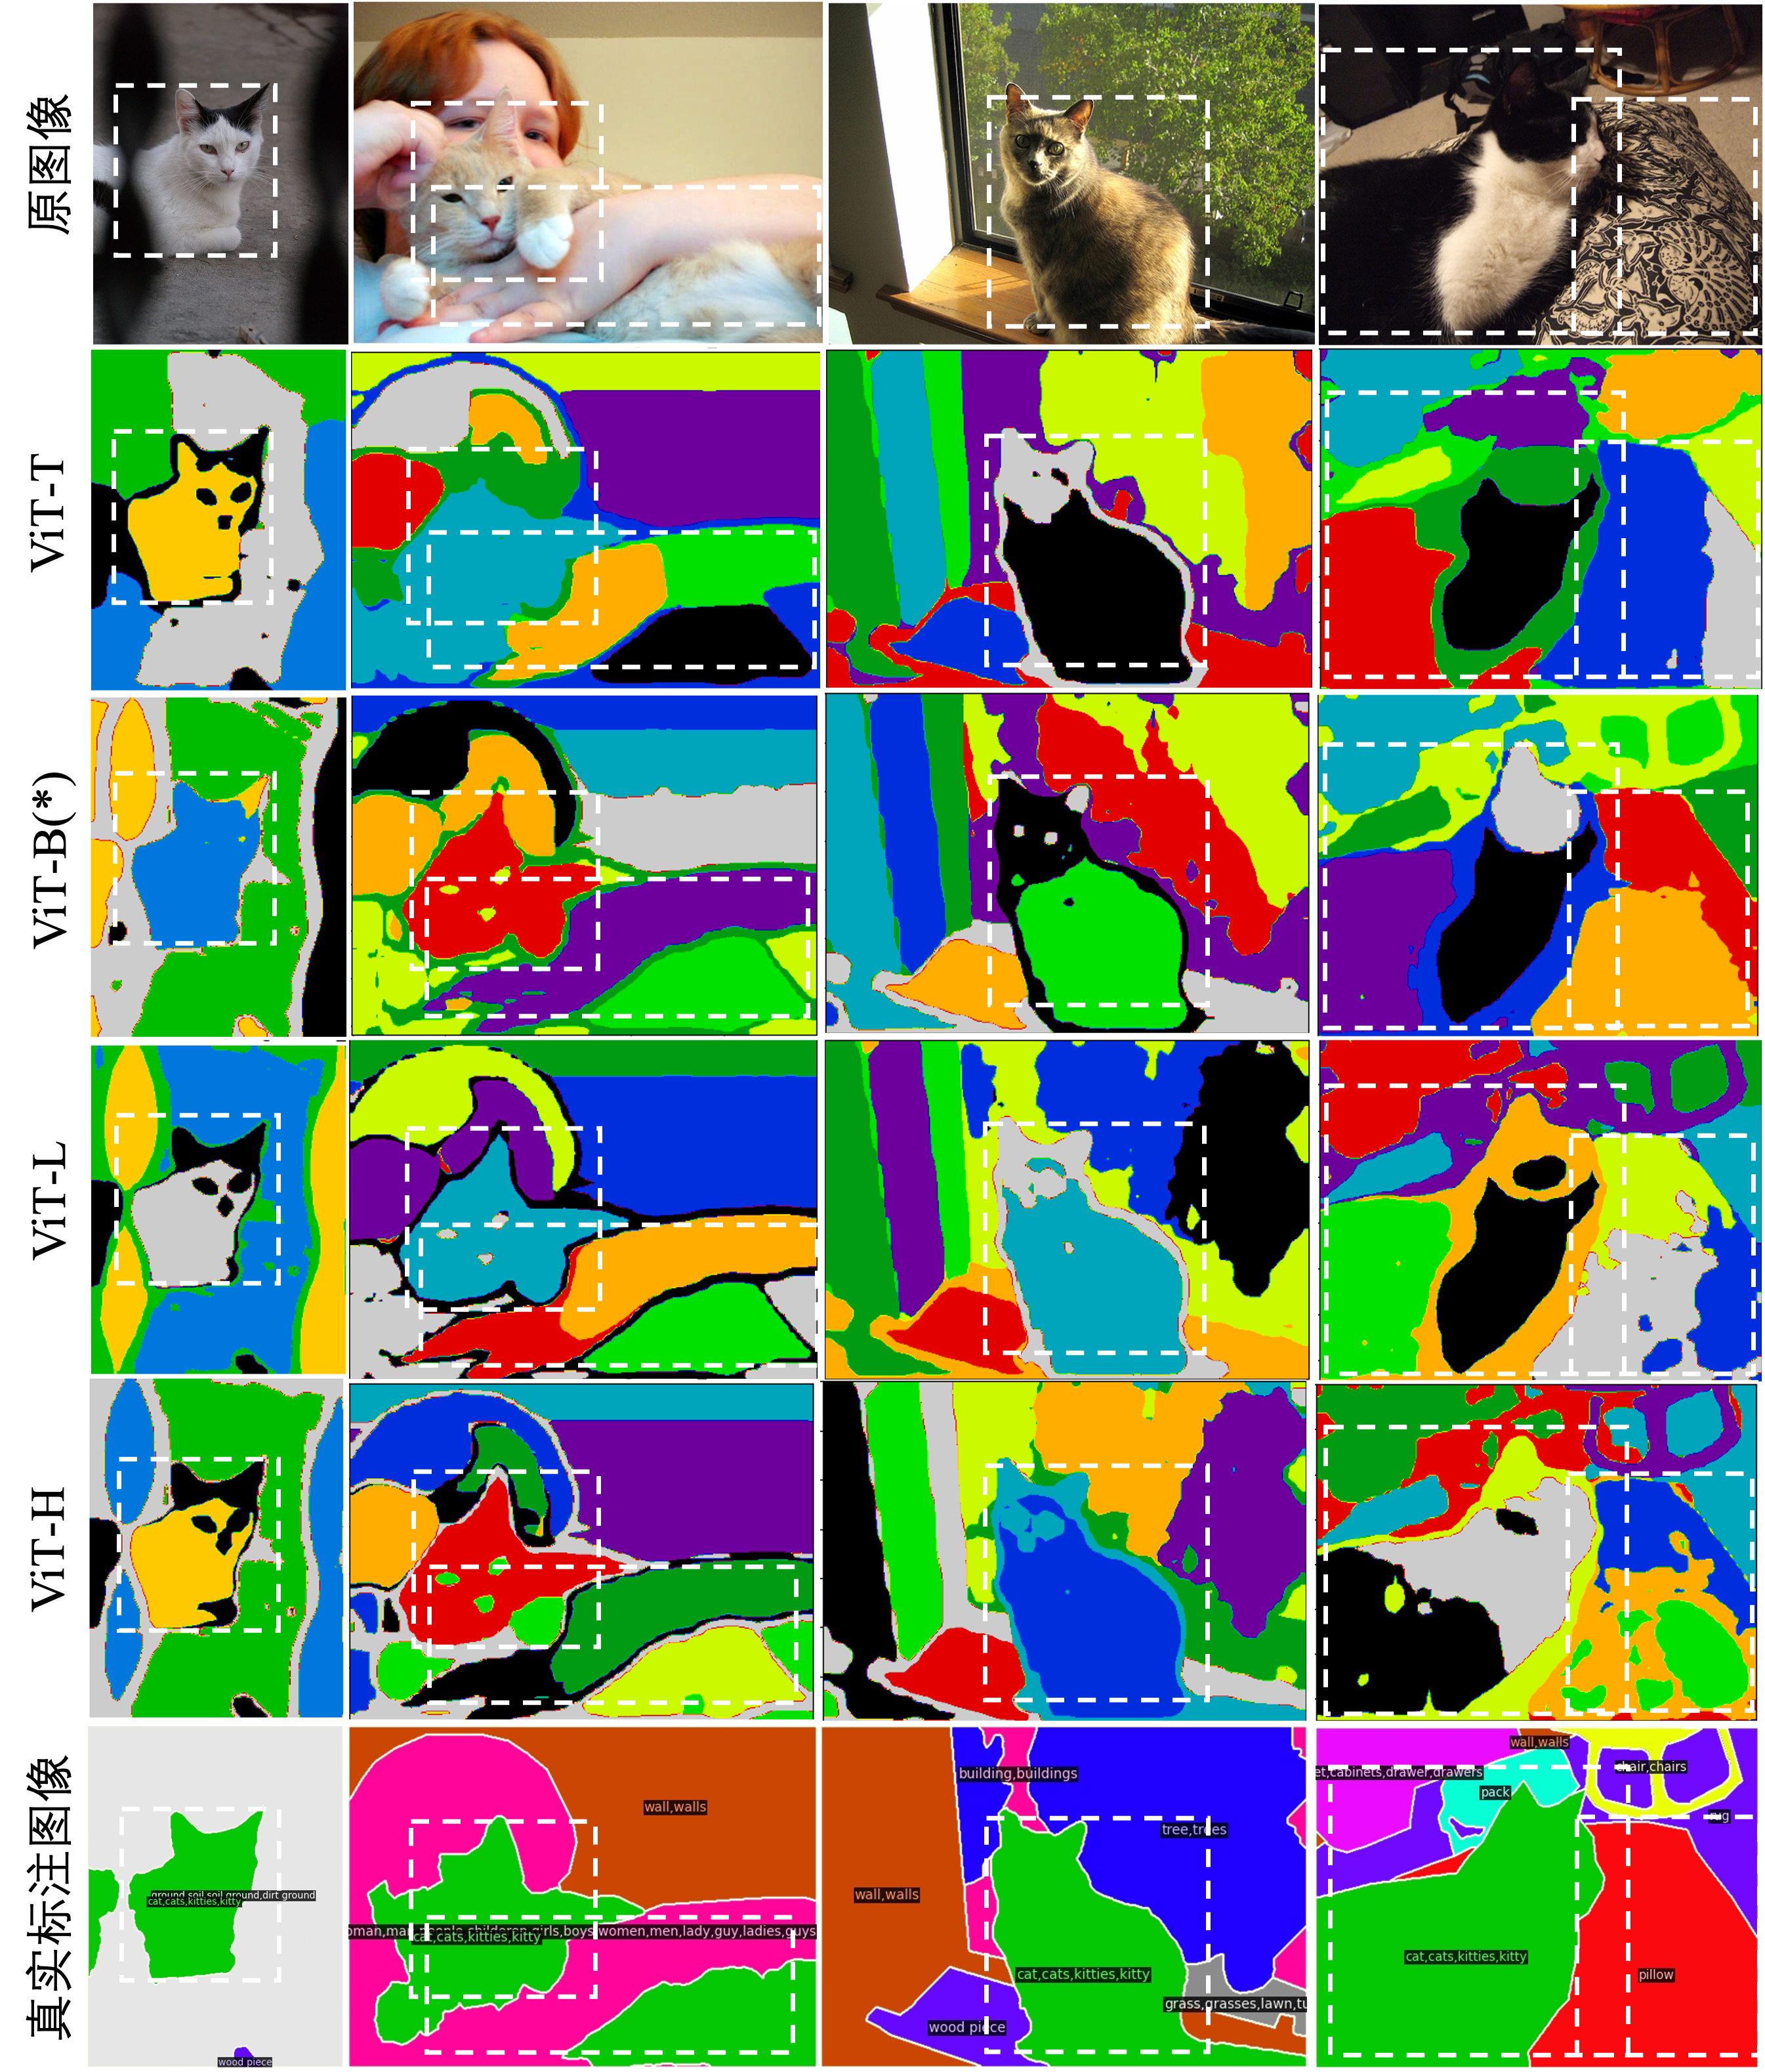
\includegraphics[width=0.65\textwidth]{figures/cmpf/sam_variants.png}
    \bicaption[fig:sam_variants]{}{不同SAM编码器在PC-459数据集上的特征嵌入k-means聚类可视化}{Fig.}{K-means clustering visualization of SAM encoder feature embeddings on PC-459}
\end{figure}

图~\ref{fig:sam_variants}给出了不同SAM图像编码器在PC-459数据集上的特征嵌入k-means聚类可视化。ViT-B编码器展现出更优的实例级连通性理解，在精确分割与实例连通之间取得了良好的平衡，与定量结果一致。

表~\ref{tab:layer_cmpf}探究了Query Injector在不同解码器层注入SAM 特征对性能的影响。CLIP的$1/8$分辨率特征对应解码器层$3,6,9$，实验表明在该分辨率注入SAM特征能获得最佳效果。这说明Query Injector应在解码器的中后段介入，使新引入的空间查询在后续层中与CLIP特征充分交互，从而实现多轮语义精炼。

\begin{table*}[!htbp] \centering
    \bicaption[tab:layer_cmpf]{}{Query Injector插入层数对性能的影响}{Table}{Impact of injection layer in decoder}
    \vspace{0.5em}\centering\wuhao
    \setlength{\tabcolsep}{10pt}
    \resizebox{.9\textwidth}{!}{%
        \begin{tabular}{cccccccc}
            \toprule
            \multirow{2}{*}{特征尺度（插入层）} & \multirow{2}{*}{Layers} & \multicolumn{3}{c}{COCO (Seen)} & \multicolumn{3}{c}{Cityscapes} \\
            \cline{3-8}
             &  & PQ & AP & mIoU & PQ & AP & mIoU \\
            \midrule
            1/32 (1, 4, 7) & 1, 4, 7 & 52.6 & 42.7 & 62.6 & \textbf{40.4} & 20.8 & 53.0 \\
            1/16 (2, 5, 8) & 2, 5, 8 & 52.5 & 42.5 & 62.4 & 40.1 & 20.7 & 53.3 \\
            1/8 (3, 6, 9) & 3, 6, 9 & \textbf{52.7} & \textbf{42.8} & \textbf{62.7} & 40.0 & \textbf{21.6} & \textbf{54.0} \\
            \bottomrule
        \end{tabular} }%
\end{table*}


% 图~\ref{fig:sam_atten}则给出了SAM在box提示下生成的分割掩码概率分布热力图。结果表明，SAM在给定box提示时能够对目标物体产生高注意力并有效抑制边缘区域，展现出稳健的零样本泛化能力，定性地验证了其在边界描绘方面的优势。

% \begin{figure}[!htbp]
%     \centering
%     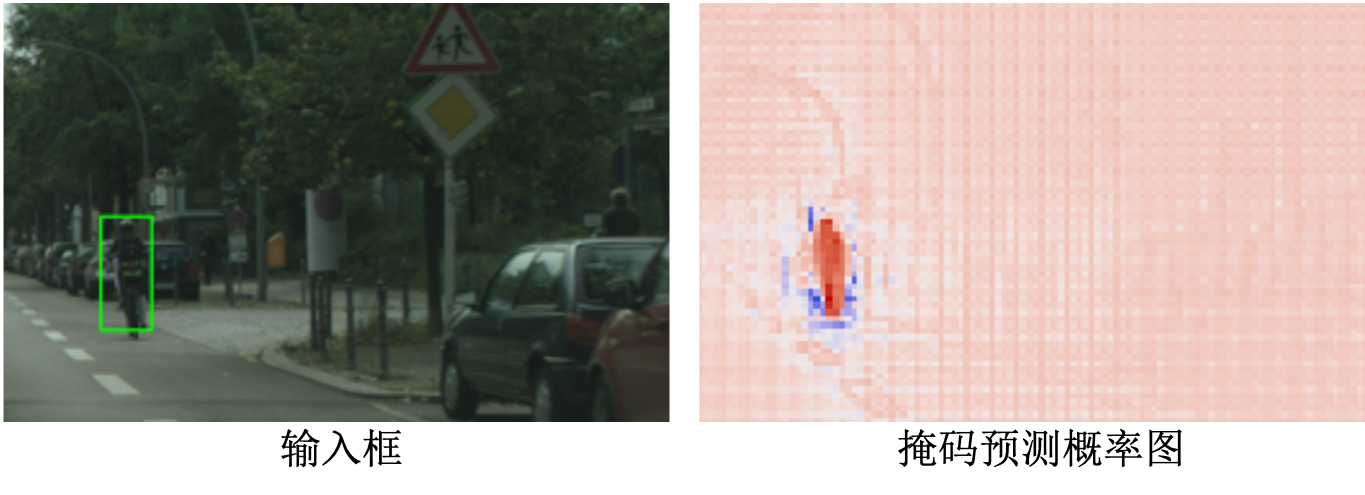
\includegraphics[width=0.75\textwidth]{figures/cmpf/sam_atten.png}
%     \bicaption[fig:sam_atten]{}{SAM在box提示下生成的分割掩码概率分布热力图}{Fig.}{Probability distribution heatmap of SAM-generated segmentation masks under box prompting}
% \end{figure}


% 图~\ref{fig:failure_case}展示了在PC-459数据集上的典型失败案例。多数错误源于三类原因：语义歧义（如“wood-piece”与“stick”的相似性）、粒度不匹配（预测与标注之间的尺度差异）以及细长物体的模糊边界（如“pole”）。这些案例反映了开放词汇分割任务本身的固有挑战，不影响前述结果的可靠性。

% \begin{figure}[!htbp]
%     \centering
%     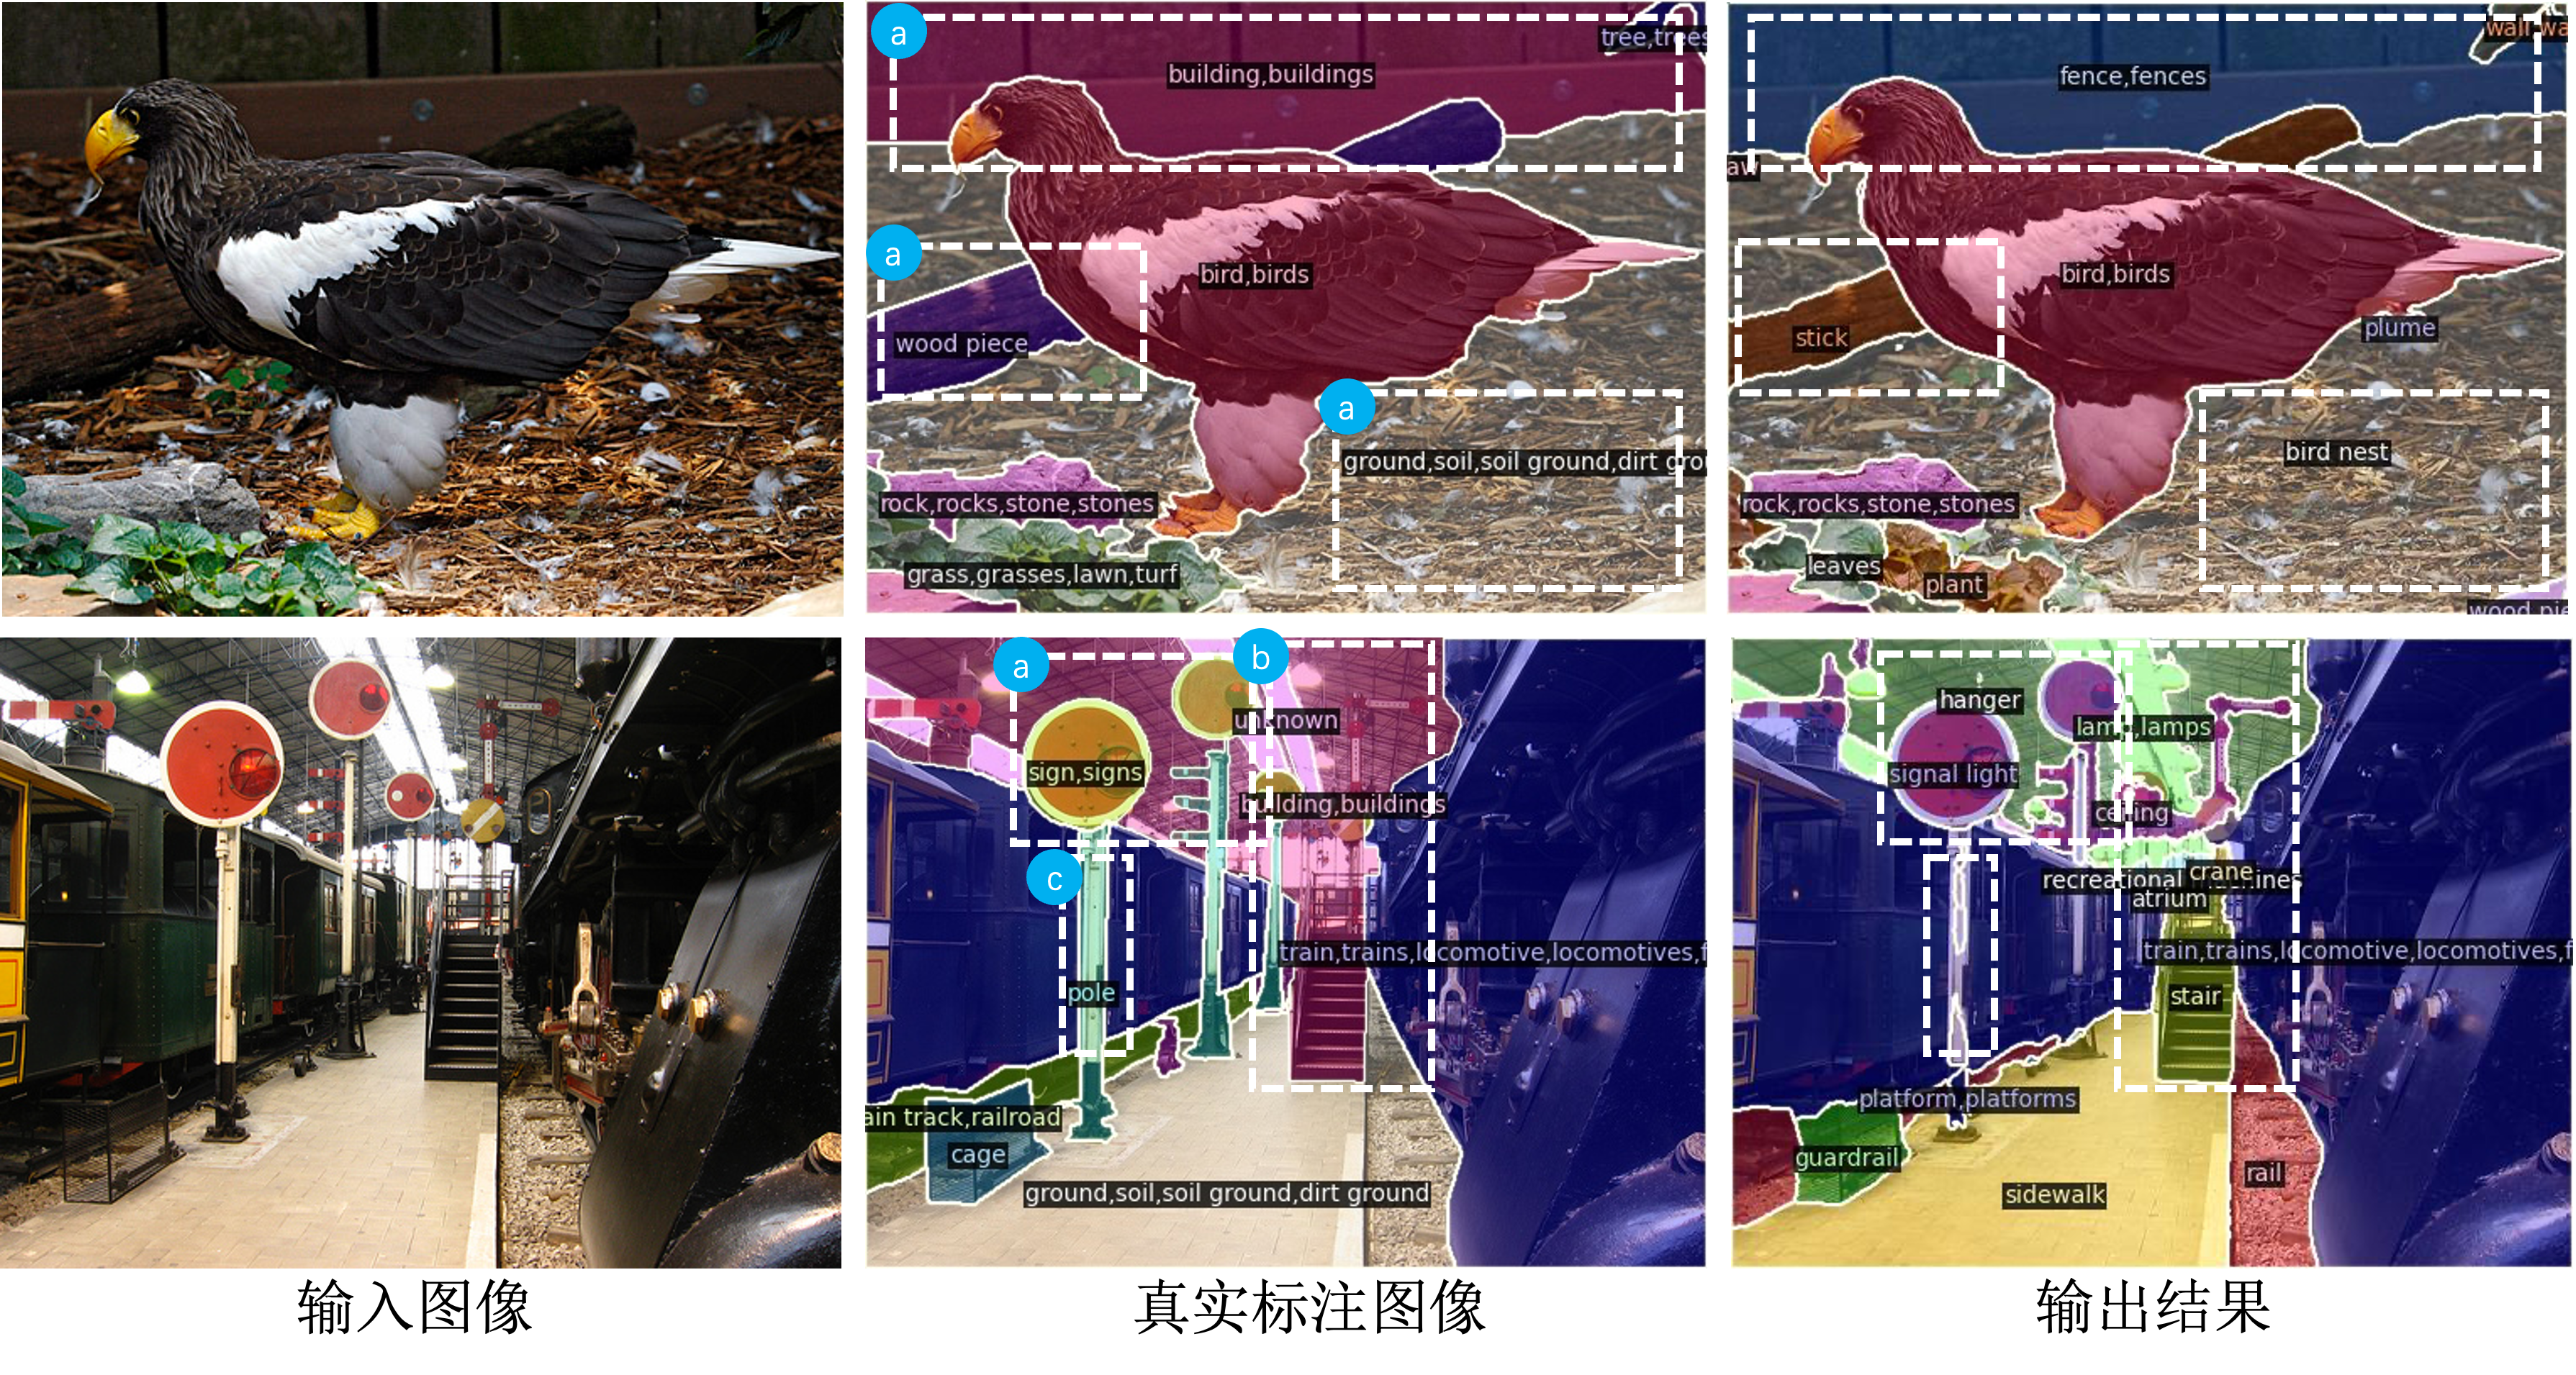
\includegraphics[width=0.85\textwidth]{figures/cmpf/fail_case.png}
%     \bicaption[fig:failure_case]{}{PC-459数据集上的典型失败案例：(a) 语义歧义；(b) 粒度不匹配；(c) 模糊边界}{Fig.}{Failure case examples on PC-459: (a) semantic ambiguity; (b) granularity mismatch; (c) ambiguous boundaries}
% \end{figure}

% \noindent\textbf{(4)推理速度与参数量对比}
\begin{table*}[!htbp]\centering
    \bicaption[tab:speed_cmpf]{}{CMPF与FC-CLIP的推理速度与参数量对比（单卡A100）}{Table}{Inference speed and parameter analysis}
    \vspace{0.5em}\centering\wuhao
    % \setlength{\tabcolsep}{2pt}
    % \resizebox{.5\textwidth}{!}{
        \begin{tabular}{lcccccc}
            \toprule
            \multirow{2}{*}{方法} & \multicolumn{2}{c}{ADE20K} & \multicolumn{2}{c}{A-847} & \multicolumn{2}{c}{参数 (M)} \\
            \cline{2-7}
             & PQ & FPS & PQ & FPS & 冻结 & 可训练 \\
            \midrule
            FC-CLIP~\cite{yu2023convolutions} & 25.1 & 2.7 & 14.0 & 3.1 & 200.0 & 21.0 \\
            SCAN~\cite{liu2024open} & -- & -- & 14.0 & 0.9 & 731.6 & 158.7 \\
            EOV-Seg~\cite{niu2025eov} & 24.5 & 11.6 & 12.8 & 11.8 & 203.7 & 21.8 \\
            \textbf{CMPF} & \textbf{25.9} & 2.2 & \textbf{14.4} & 2.9 & 293.5 & 26.5 \\
            \bottomrule
        \end{tabular}
        % }
\end{table*}


引入SAM并没有引入额外的推理开销，表~\ref{tab:speed_cmpf}给出了CMPF与同类CLIP基方法的推理速度与参数量对比。CMPF与FC-CLIP和SCAN的推理速度相当，额外引入的参数量带来了明显的精度提升，体现了良好的精度—效率权衡。


\section{本章小结}

本章围绕开放词汇分割中视觉—语言模型掩码质量不足的问题，沿训练期融合与推理期集成两个角度展开治理。训练期融合通过查询注入与特征注入两类轻量模块，在 Transformer 解码器内部实现分割基础模型的空间定位先验与视觉—语言模型的开放词汇语义先验的深度融合，且全程保持两个基础模型参数冻结；推理期集成通过类别与掩码的两阶段策略融合分割基础模型的零样本掩码预测，专门用于提升未见类别的分割质量。消融分析表明训练期特征融合是性能提升的主要驱动力，推理期掩码集成在其基础上提供互补增益。八个基准上的实验验证了方法在数据效率与泛化能力上的优势。

% Local Variables:% Local Variables:
% TeX-master: "../thesis"
% TeX-engine: xetex
% End:

% !Mode:: "TeX:UTF-8"

\chapter[基于证据锚定的多维语义理解基准]{基于证据锚定的多维语义理解基准}[]
\chaptermark{基于证据锚定的多维语义理解基准}

\label{chap:5}
\setcounter{footnote}{0}
\renewcommand{\thefootnote}{\arabic{footnote}}

% 图表与公式编号按章重置并显示为 "章-序"（X-Y）格式，
% 由 book.cls 的 \newcounter{figure}[chapter] / \@addtoreset{equation}{chapter}
% 与 hithesisbook.cls 的 \thefigure / \thetable 定义共同保证；
% 此处不可再调用 \counterwithin，它会把编号改写为 "X.Y" 且全局泄漏到后续章节。

\section{引言}

前几章以数据分布和类别词表的变化为线索，研究模型如何在目标条件改变时保持识别与定位能力。然而，目标任务对模型的要求并不止于回答图像中有什么；在需要解释情感的场景中，模型还须说明判断依据，并使解释与可见的视觉线索相吻合。艺术情感理解集中体现了这一要求：作品中的对象内容、色彩、构图和文化语境可能共同影响情感表达，单凭情感标签难以判断模型是否真正理解了作品。本章据此将研究视角从提升迁移表现转向评估既有能力，以艺术情感推理为例，构建多层级评测基准，考察多模态大语言模型面对更高语义理解要求时的适用范围与失效环节。

近年来的研究使得多模态大语言模型 MLLM 在通用视觉理解任务上取得了长足进展，闭源与开源模型在视觉问答~\cite{kuang2025natural,tang2025mtvqa}、图表推理~\cite{masry2025chartgemma}、OCR 导向的文档理解~\cite{yang2025cc,ye2023mplug}等多个方向上已展现出接近人类的事实识别与文字定位能力~\cite{mmbench2023}。然而，当任务从“识别图像中可被显式命名的实体”升级到涉及意图、情感、文化语境与审美判断的高阶语义推理时，这一类模型的能力出现了明显的缺口。语义类内容与事实类内容存在本质差异：受主观性、抽象性与文化语境三重影响，语义类内容的可靠解释难以被“事实正确性”或“流畅表述”等单一维度度量；高阶语义理解所需的细粒度证据化标注（如“左上方冷色笔触营造孤寂氛围”）在大规模预训练语料中极为稀缺~\cite{aesexpert2024}，导致模型缺乏从局部视觉元素到整体情感语义的可追溯推理路径，其生成结果常表现为语言流畅但缺乏视觉证据支撑的“流畅的虚构”~\cite{eemobench2025}。这一从显式视觉事实到高阶语义推理的跨越，对当前以视觉—语言对齐为核心的 MLLM 提出了全新的能力要求。

这一缺口同时具有科学价值与应用价值。从科学角度看，高阶语义理解评测能够压力测试 MLLM 是否具备从字面识别走向“可解释的、有证据支撑的”语义推断的能力，从而揭示模型在跨模态语义组合与文化语境建模上的真实水平~\cite{liu2025emer}。从应用角度看，博物馆导览~\cite{Balauca_2025_ICCV}、艺术教育~\cite{LEE2024100297}以及创意辅助等场景越来越依赖 MLLM 对作品进行自动化的情感解读与讨论；缺乏严格评测协议支撑的“视觉推理”声称很可能高估了模型真实的情感认知能力。

现有研究在证据锚定与评测维度建模两个层面均存在不足。在证据锚定层面，面向情感的视觉数据集，如 ArtEmis~\cite{achlioptas2021artemis}、EmoSet~\cite{yang2023emoset}、EmoArt~\cite{emoart2025}、EEmo-Bench~\cite{eemobench2025}，或提供粗粒度的情感分类标签，或关注艺术图像的美学属性，或生成情感化描述，但普遍未将语义归因与视觉证据进行细粒度绑定；在评测维度建模层面，面向美学的基准，如 AES-Expert~\cite{aesexpert2024}、ArtiMuse~\cite{cao2025artimuse}，聚焦于美学质量评分与专家级描述生成，仍沿用单维分类或简短问答形式，未能系统拆解互补的认知子维度。两类工作的共同缺口在于：尚未存在一个能够将高阶语义理解从“感知线索”逐层追溯到“情感判断”再到“证据化解释”的诊断型评测基准。

为填补上述空白，本章构建面向艺术情感推理的多层级评测基准 AER-Bench。与已有工作相比，AER-Bench 的核心特征在于：它将高阶语义理解明确地拆解为四个互补的认知子维度——感知维度层、情感与 VAD 层、推理层与描述层，并将每一层级实例化为可重复生成的评测任务，从而在证据锚定与评测维度建模两个层面同时实现对 MLLM 的细粒度诊断。

\begin{figure}[!htbp]
    \centering
    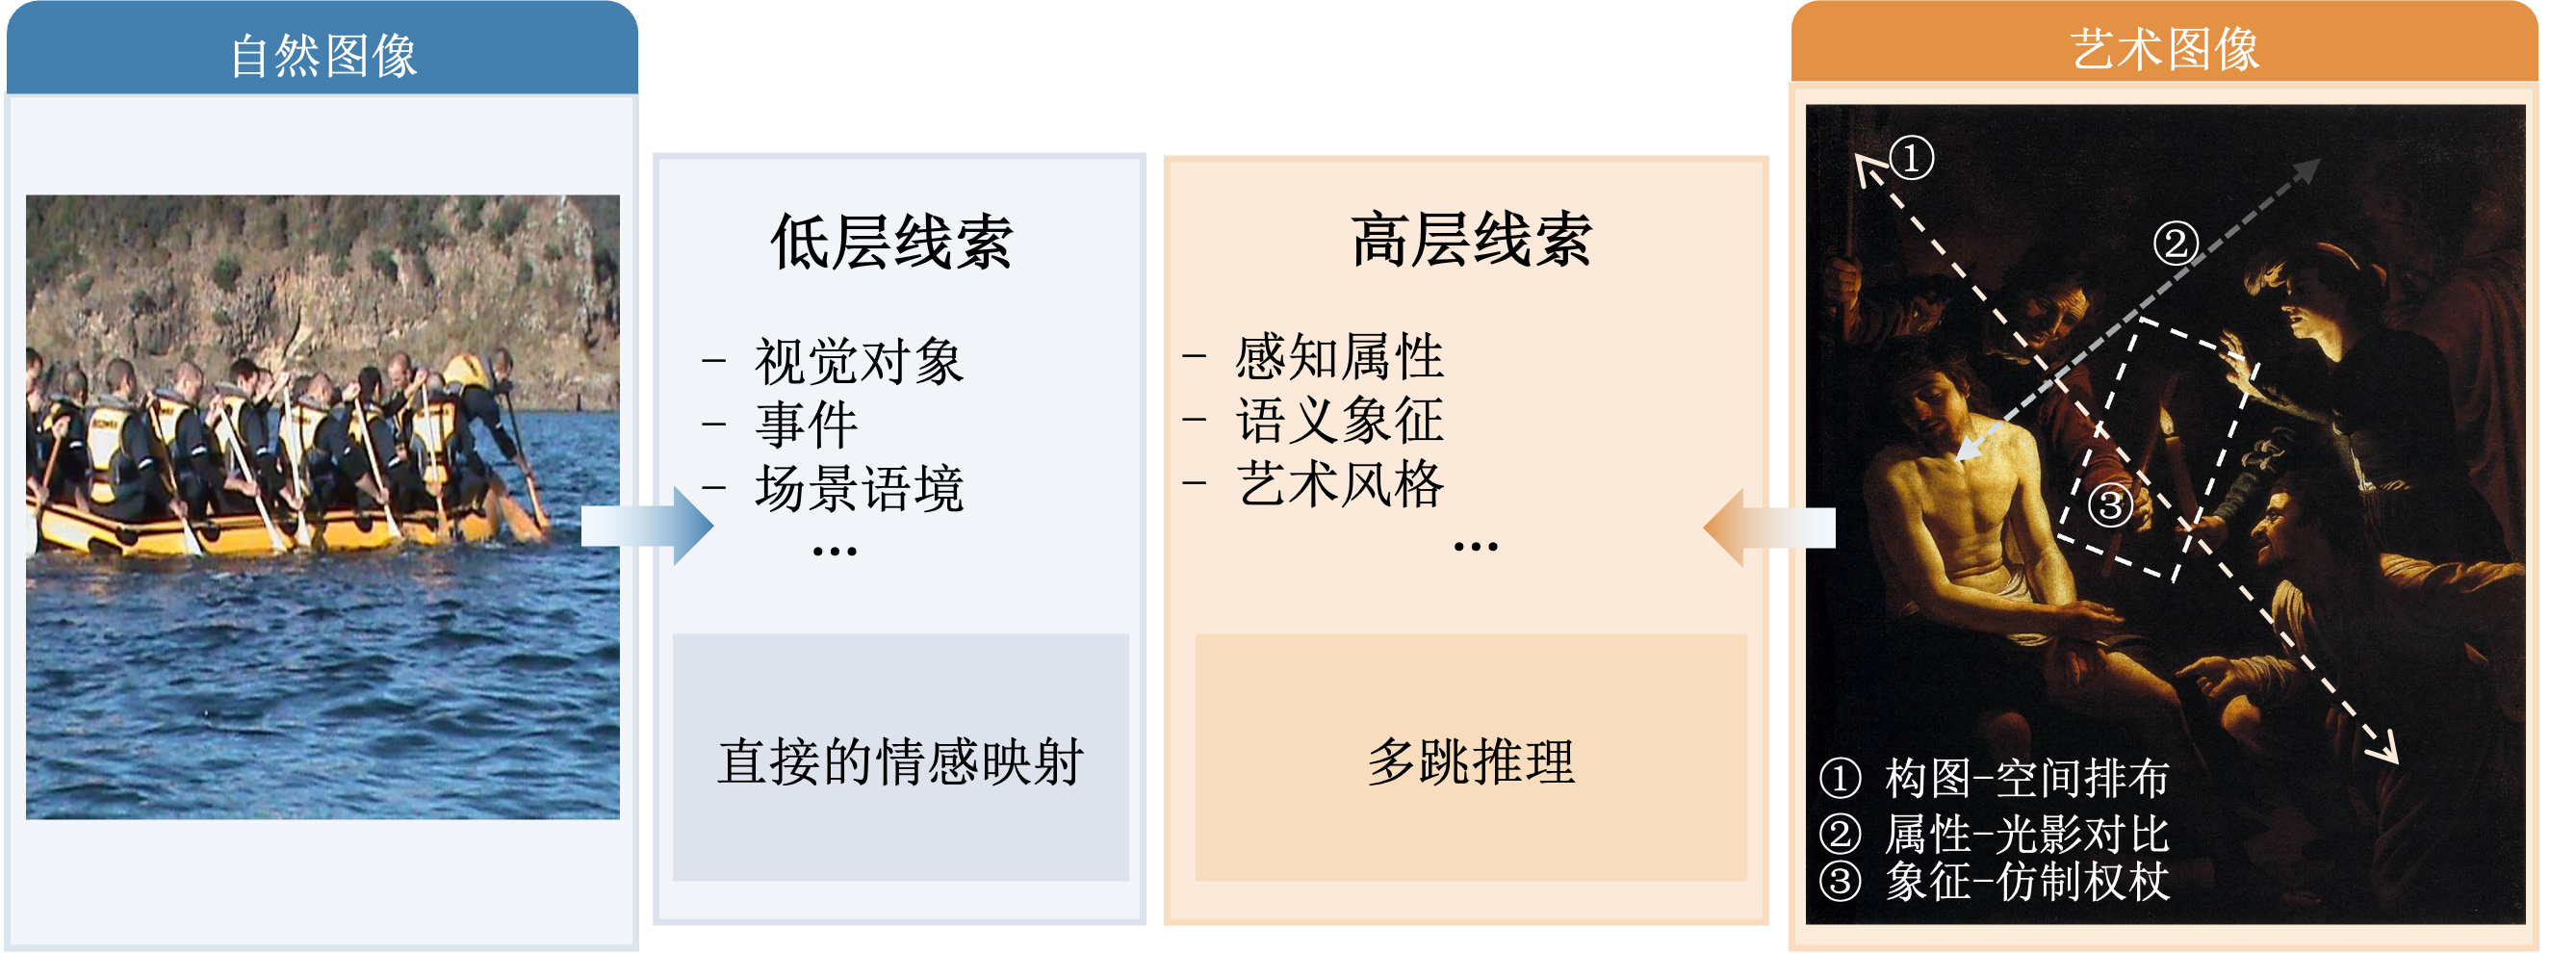
\includegraphics[width=0.92\textwidth]{figures/aerbench/moti.png}
    \bicaption[fig:chap5_main_comparison]{}{自然图像与艺术图像情感推理的差异：从显式实体线索到隐式形式线索的跨越}{Fig.}{Comparison between ordinary image emotion reasoning and art image emotion reasoning, highlighting the shift from explicit cues to implicit aesthetic cues}
\end{figure}

AER-Bench 通过以下方式实现上述评测目标：在数据层面，从覆盖八类艺术风格的 2,058 件作品中构建具有风格多样性的图像集合；在标注层面，采用 GPT-4o~\cite{achiam2023gpt} 辅助的结构化标注框架，结合 CLIP~\cite{radford2021learning} 相似度过滤与多轮人工核验，确保标注的内部一致性；在任务层面，采用固定模板而非自由提示生成评测题目，并通过单图与双图两种设置同时考察模型的图像内推理能力与图像间关系推理能力。基准最终产出 24,792 个单图任务与 9,999 个配对任务；在模型层面，覆盖 4 个闭源与 10 个开源 MLLM，合计 14 个代表性模型的系统评测，从而支撑跨模型、跨设置的能力对比与失败模式分析。

本章的主要贡献可总结为以下三点：
\begin{enumerate}
    \item AER-Bench 多层级诊断基准：构建首个面向艺术情感推理的多层级诊断型基准，通过结构化的“感知—情感—推理—描述”四级标注体系对艺术情感理解过程进行显式分解，并据此生成可重复、可对齐的评测任务，覆盖 2,058 件作品、24,792 个单图任务与 9,999 个配对任务。
    \item 统一评测协议：融合确定性度量与基于评分的语义评判，将客观题与开放式题置于同一评测框架下，覆盖感知单选、情感排序、评分、配对推理与开放式描述多种任务形式，同时支撑单图与双图两种设置的能力诊断。
    \item 模型系统评测与瓶颈揭示：在 14 个代表性 MLLM 上系统评测，揭示当前 MLLM 在艺术情感理解上的核心瓶颈——能够生成看似合理的情感标签或流畅的情感描述，但难以将这些输出锚定到具体的感知线索、上下文证据与表达模式上，体现出在“基于证据的解释”层面的系统性能力缺口。
\end{enumerate}

\section{面向图像情感语义的基准设计与评测}

\label{sec:chap5_benchmark_design}

AER-Bench 将艺术情感理解形式化为一个由低到高的四级能力体系：感知维度层（Perception）刻画从低层视觉形式到高层情感的中介证据，情感与 VAD 层（Emotion \& VAD）刻画情感判断本身，推理层（Reasoning）刻画从证据到情感的解释过程，描述层（Description）刻画对作品整体情感氛围的综合表达。这一四级体系直接对应数据标注与任务生成的层级结构，使模型的能力缺陷能够被精确定位到具体层级。

\begin{figure}[!htbp]
    \centering
    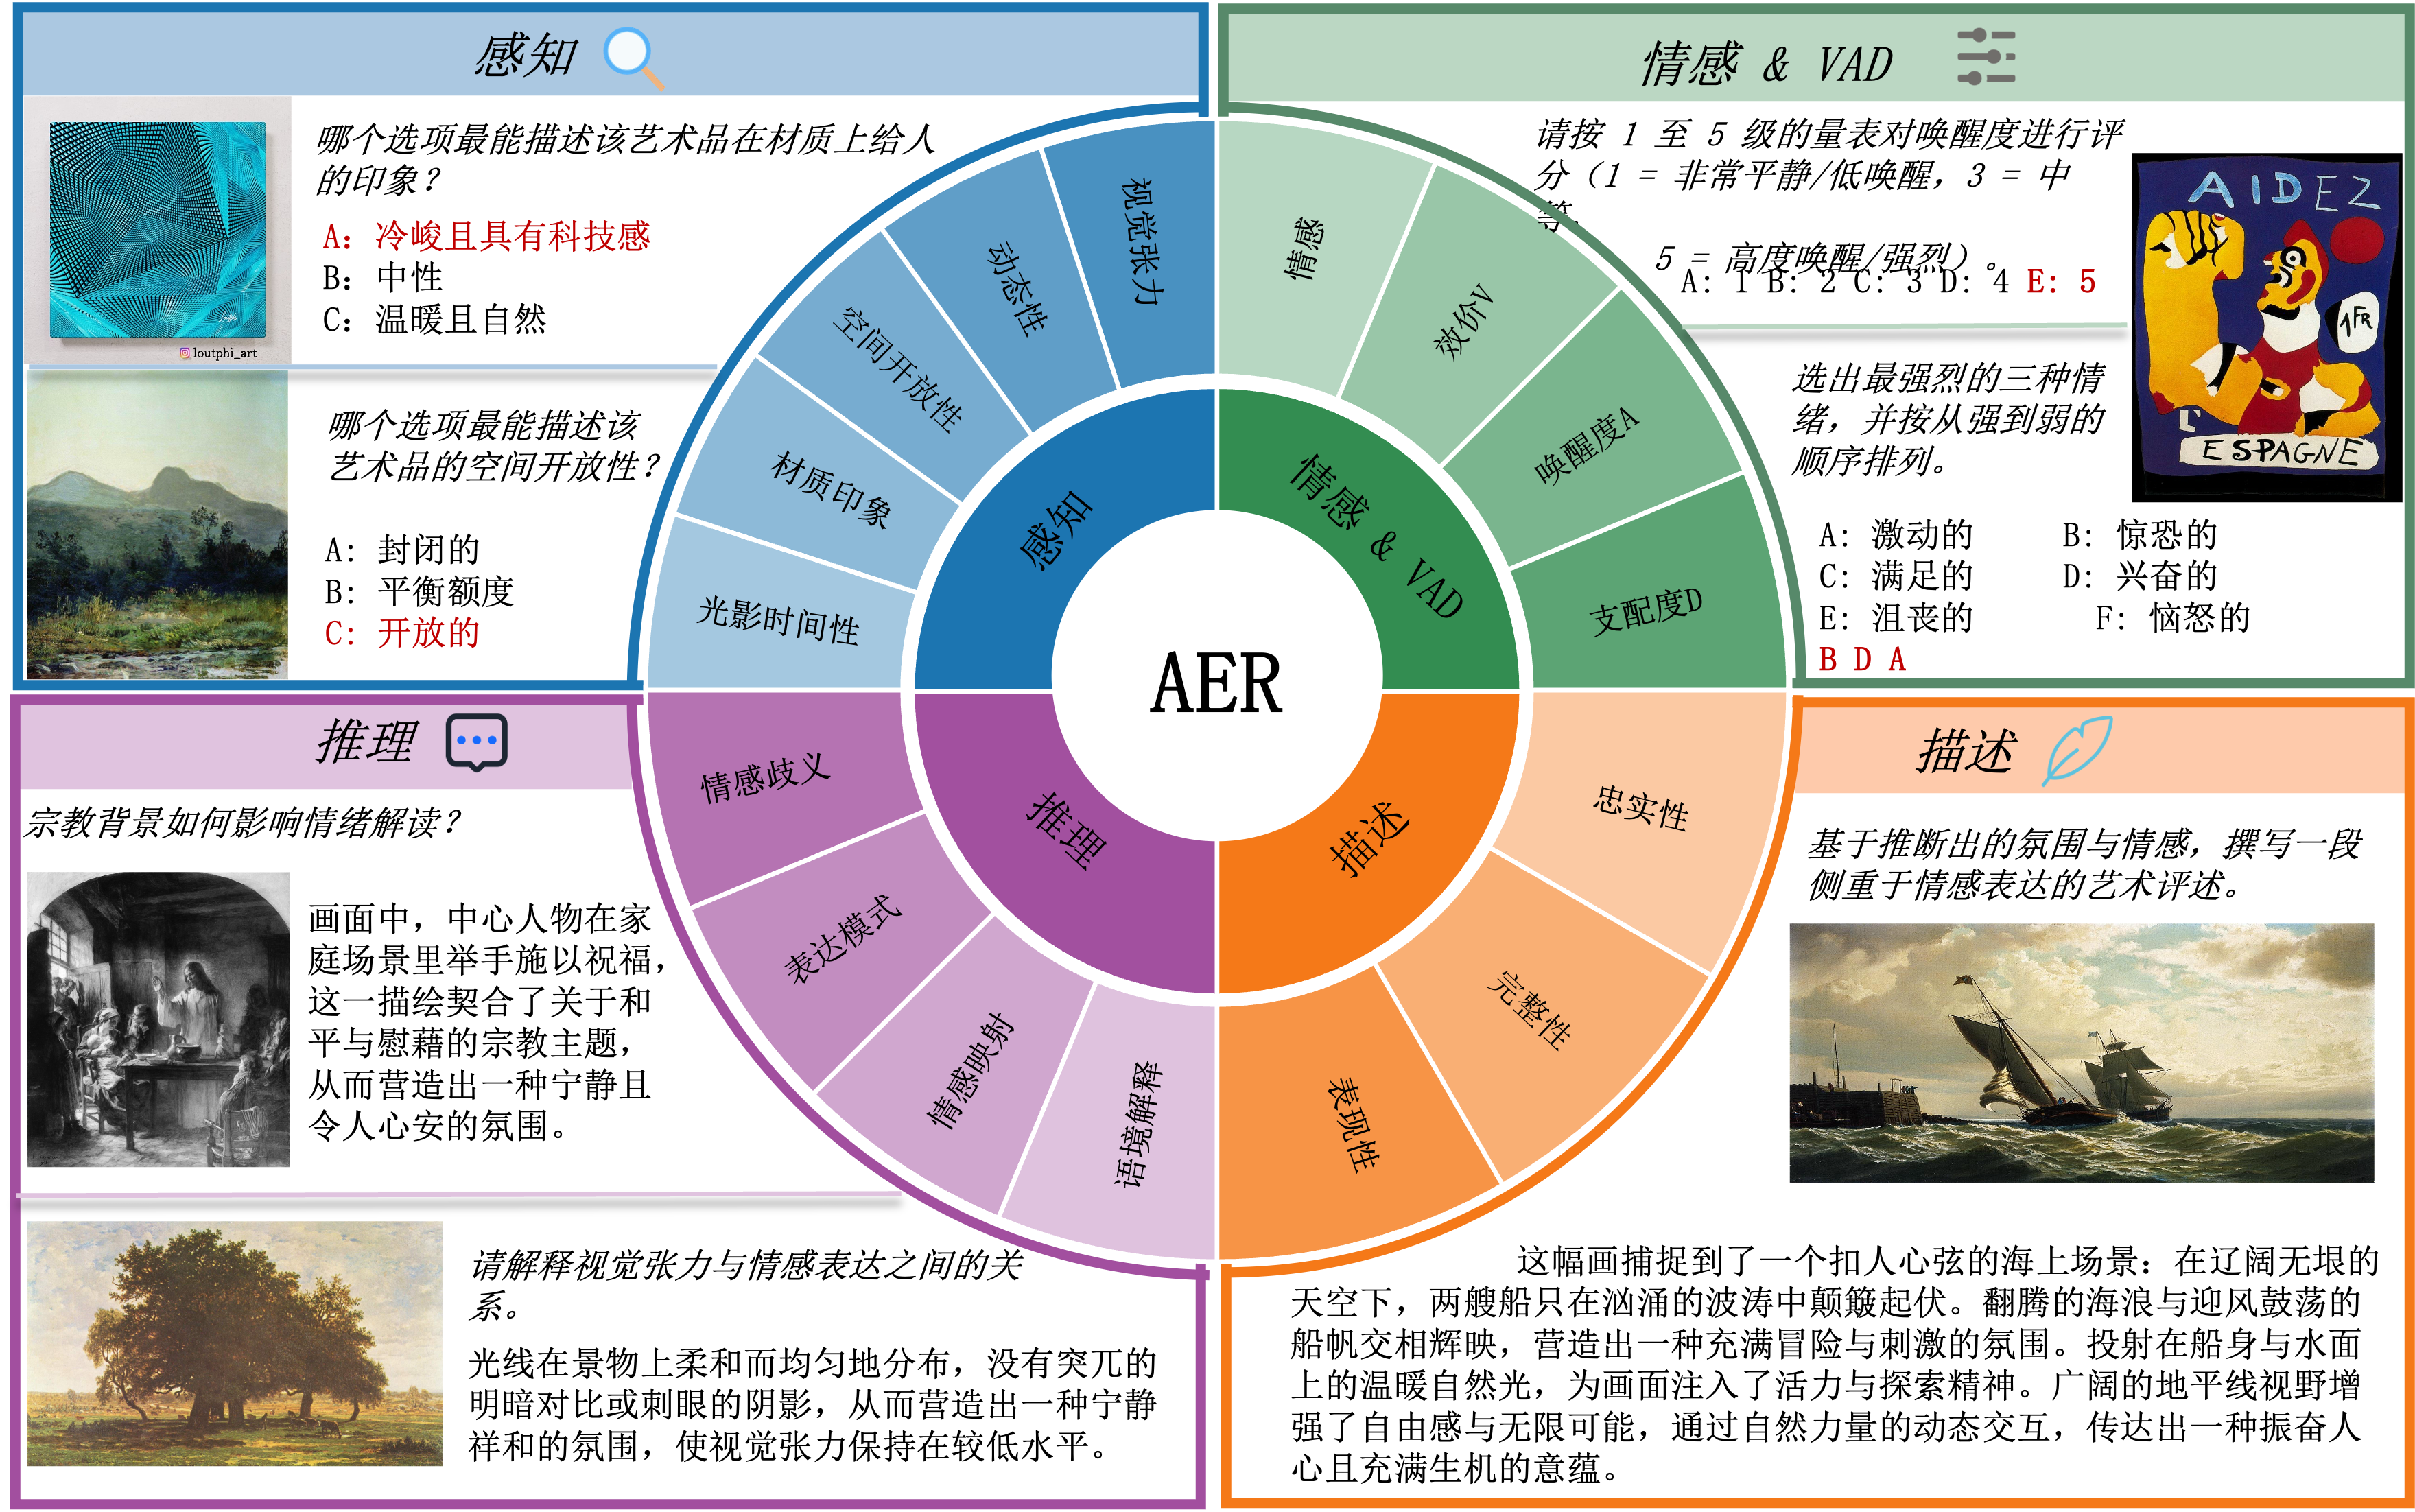
\includegraphics[width=0.95\textwidth]{figures/aerbench/main.png}
    \bicaption[fig:chap5_comp]{}{AER-Bench 评测体系总览}{Fig.}{Overview of the AER-Bench design}
\end{figure}

\subsection{多维语义层级建模}

\label{sec:chap5_four_layer_representation}

本节按由低到高的顺序，将艺术情感推理过程形式化为感知维度、情感与 VAD、证据锚定推理与综合氛围描述四个层级，并使每层既可独立评测、又可与上一层形成依赖关系，从而支撑对模型能力的层级化诊断。

感知维度层作为低层视觉形式通往高层情感的中介证据，借鉴 Arnheim《Art and Visual Perception》中关于“形式—情感关系”的论述~\cite{arnheim1954art}与 Zhao 等人提出的“艺术原则特征”~\cite{zhao2014exploring}，将艺术作品的形式特征操作化为视觉张力（visual tension）、动态性（dynamism）、空间开放性（spatial openness）、材质印象（material impression）与光照时间性（light temporality）五个可标注维度；相较于纯粹基于色彩、纹理等低层视觉元素的特征~\cite{lu2012shape}，感知维度更接近艺术创作与艺术评论所使用的描述语言，能够同时服务于标注与评测。

情感与 VAD 层在感知维度所揭示的形式证据之上，刻画模型对作品情感状态的直接判断。离散标签方面，采用 12 个共享情感词（兴奋aroused、激动excited、快乐happy、悲伤sad、无聊bored、疲惫tired、惊恐alarmed、恼怒annoyed、沮丧frustrated、高兴glad、满足contentment、平静calm）构成的有限集合，覆盖从高唤醒度到低唤醒度、从正效价到负效价的完整情感谱系~\cite{warriner2013norms,eemobench2025}；连续维度方面，采用情感心理学中广泛使用的 效价--唤醒度--支配度（VAD）三维评分~\cite{warriner2013norms}，三维均采用 1--5 量表，并与 Warriner 等发布的 13,915 词英语 VAD 词典在取值范围与情感语义上保持一致，便于在词级别进行跨数据集的语义对齐，三个维度在 1--5 量表上的锚点定义见附录~\ref{app:aerbench_supplement}。离散标签保证情感判断的可解释性，VAD 维度保证与情感心理学已有范式的可对接性，二者共同支撑模型在情感粒度上的多尺度能力评测。

证据锚定推理层进一步评估模型能否将上述情感判断锚定到具体的视觉证据与上下文线索上，而非仅给出情感标签本身。借鉴 Panofsky 的图像学分析框架~\cite{panofskyiconography}与艺术评论中“形式—语境—意图”的分析路径，AER-Bench 将推理进一步细分为四个子维度：（1）情感映射（affective mapping）评估模型能否显式说明特定感知维度如何支撑其情感判断；（2）语境（context）评估模型在涉及历史、文化、宗教、政治或符号背景时能否恰当地调整情感解释；（3）多义性（ambiguity）评估模型在多实体、主体—背景或形式—内容冲突情境下能否辨识与权衡；（4）隐性表达（implicit impression）评估模型能否识别作品以直接、间接或混合方式传达情感。

综合氛围描述层在前三个层级之上，评估模型对作品整体情感氛围的综合表达能力，要求描述同时覆盖表现性（expressiveness，是否流畅且富有情感表现力）、完整性（completeness，是否覆盖主要情感氛围与关键描述要点）与忠实性（faithfulness，是否与作品视觉证据一致、无凭空捏造）三个属性，避免出现“流畅但无证据”式的情感短语堆砌；该三元评估基准与开放词汇描述生成领域的可解释性研究~\cite{emoart2025,achlioptas2021artemis}保持一致。四个层级共同构成从“视觉证据”到“情感判断”再到“证据化解释”的完整评测链条，使模型在每一抽象层级的缺陷都能被精确定位。这一层级化结构直接体现在基准的构造流程中：结构化标注经由模板化题合成被实例化为评测任务，使能力缺陷能够被定位到具体层级，如图~\ref{fig:chap5_data_build}所示。

\begin{figure}[!htbp]
    \centering
    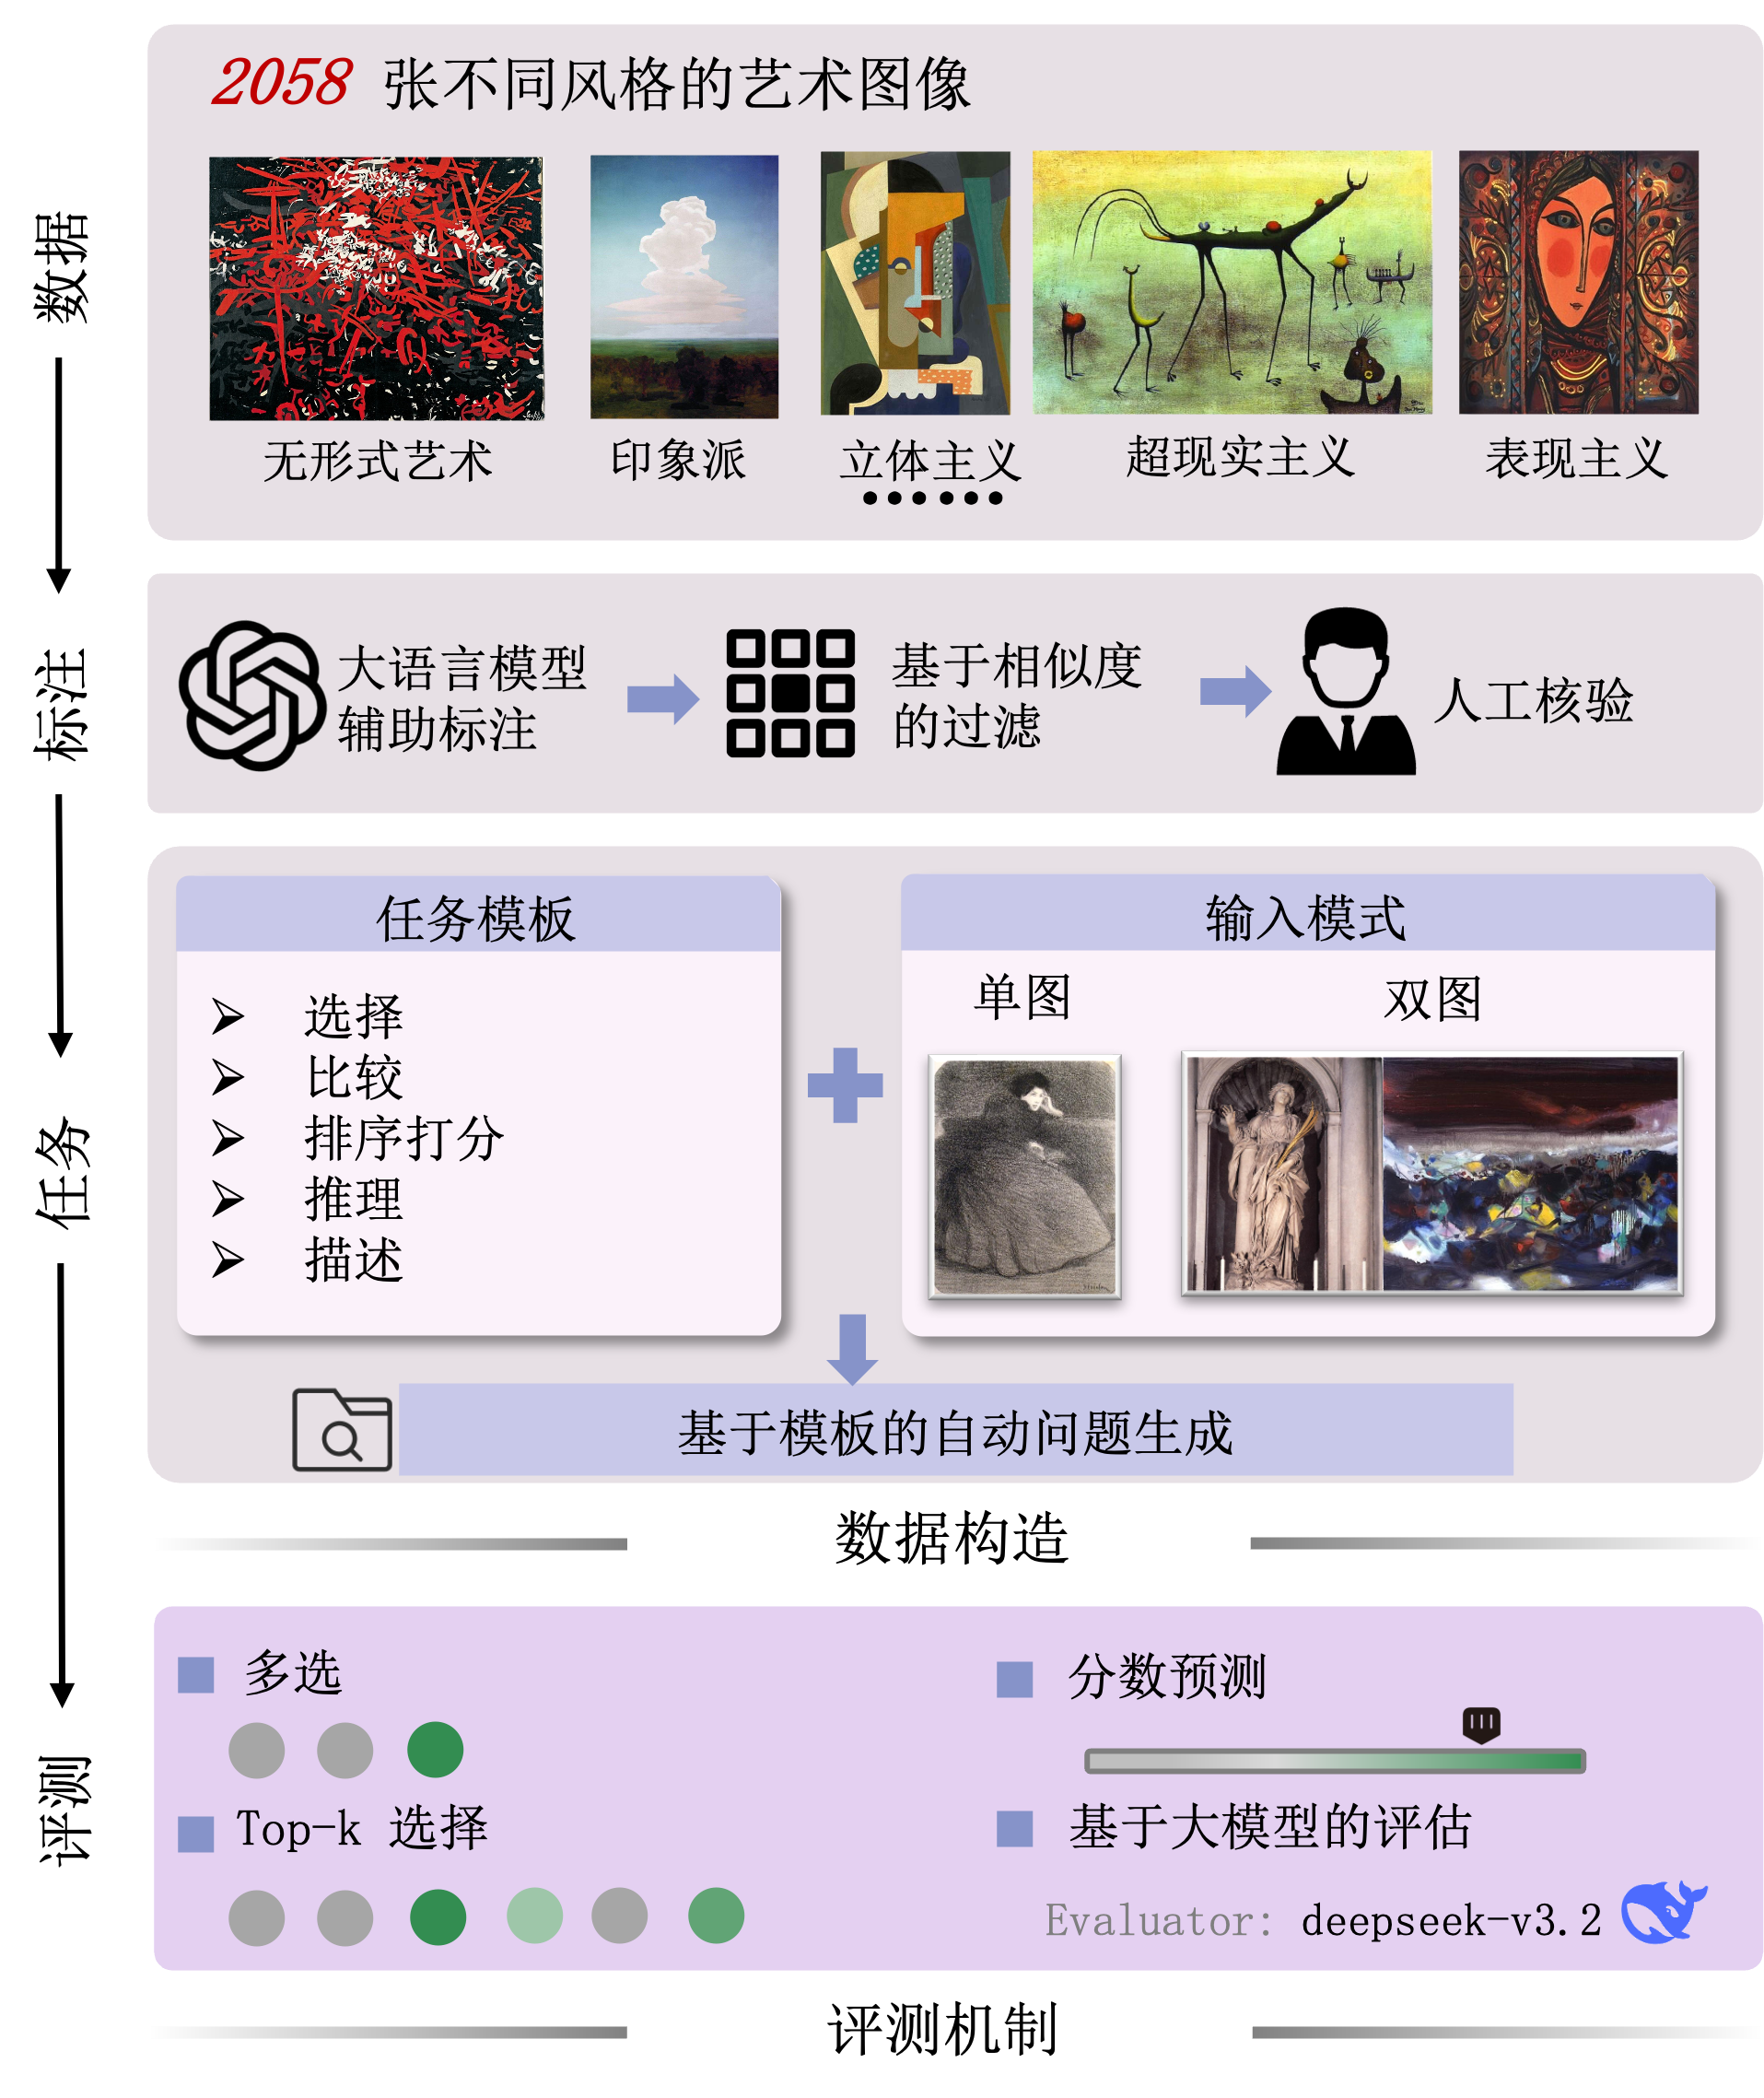
\includegraphics[width=0.65\textwidth]{figures/aerbench/data_build.png}
    \bicaption[fig:chap5_data_build]{}{AER-Bench 构造流程总览}{Fig.}{Overview of the benchmark construction pipeline}
\end{figure}

\subsection{数据质量控制与系统评测}

\label{sec:chap5_data_pipeline}

为保证视觉与风格多样性，AER-Bench 的源图像采集自 WikiArt\footnote{\url{https://www.wikiart.org/}}，这是一个覆盖从文艺复兴至当代抽象艺术的大规模在线艺术作品集合。考虑到艺术情感常常由作品的形式结构、绘画风格、象征内容与观者诠释共同决定，而非由单一显式对象承载，WikiArt 的风格多样性天然契合本基准对情感表达异质性的需求。采样过程按以下顺序执行：首先进行初始检索，在 WikiArt 上按多个时期与流派进行广泛候选抓取，最大化风格与主题覆盖；随后进行风格分层，将候选作品归入八大风格家族——现实主义、印象主义、表现主义、抽象艺术、超现实主义、象征主义、当代艺术、其他，并按比例分层采样，避免对单一艺术传统的过表征，确保下游任务不会被某一熟识的美学惯例系统性偏置；最后采用相似度过滤去除近重复样本。经过上述筛选，最终保留 2,058 件作品作为基准源集合。

AER-Bench 采用以 GPT-4o~\cite{achiam2023gpt} 为辅助的结构化标注策略：标注提示要求模型按照预定义的 JSON 模式，针对每件作品同时输出五维感知评分、情感 Top-3 与 VAD 三维、情感描述与基于证据的推理四个层级的标注，其关键指令与取值约束汇总于表~\ref{tab:chap5_prompt_summary}；为保证大规模标注的可重复性与可恢复性，标注管线引入了系统化的错误处理与断点续传机制。标注质量通过多层过滤与人工核验共同保证：
在自动过滤方面，针对单选感知题，使用 CLIP（ViT-L-14）~\cite{radford2021learning} 计算图像—选项对的相似度，仅保留真值选项在 CLIP 相似度上具有显著优势的样本，从而去除视觉不一致或歧义过大的实例；针对配对题，使用 GPT-4o 对同一对图像进行独立复核，将分歧样本对齐到模型判断，并仅保留确定且置信度足够的样本。
在人工核验方面，从全部标注中按任务类型分层随机抽样，由三位具备视觉艺术与多模态评估背景的标注员独立核验。相关结果位于表~\ref{tab:chap5_llm_judge}:标注一致性（Krippendorff's $\alpha$）超过 0.68，调整一致率（adjusted agreement， Adj.Agr）达 95.2\%，平均得分 0.79（归一化至 [0,1] 区间），证明标注能够被领域专家接受；核验的设计与评分细则见附录~\ref{app:human_verification}。


\begin{table}[!htbp]
    \bicaption[tab:chap5_llm_judge]{}{AER-Bench LLM 评判与人类专家一致性核验}{Table}{Validation of AER-Bench LLM judge against human experts}
    \vspace{0.5em}\centering\wuhao
    \setlength{\tabcolsep}{4pt}
    \begin{tabular}{lrccccc}
    \toprule
    \multirow{2}{*}{任务} & \multirow{2}{*}{N} &
    \multicolumn{3}{c}{\textit{标注核验}} &
    \multicolumn{2}{c}{\textit{LLM 评判核验}} \\
    \cmidrule(lr){3-5}\cmidrule(l){6-7}
     & &
    Hum.-$\alpha$ & Adj.\ Agr.\ (\%) & 平均 & LLM--Hum.\ $\kappa_w$ & Self-$\alpha$ \\
    \midrule
    单图推理 & 120 & 0.74 & 96.8 & 0.89 & 0.69 & 0.88 \\
    配对推理 & 120 & 0.69 & 94.3 & 0.77 & 0.58 & 0.85 \\
    情感描述 & 120 & 0.61 & 92.1 & 0.72 & 0.53 & 0.83 \\
    \midrule
    整体 & 360 & 0.68 & 95.2 & 0.79 & 0.60 & 0.86 \\
    \bottomrule
    \end{tabular}
\end{table}

\begin{table}[!htbp]
    \centering
    \bicaption[tab:chap5_prompt_summary]{}{标注与开放式评测所用提示词要点汇总}{Table}{Summary of prompts used for annotation and open-ended evaluation}
    \vspace{0.5em}\centering\wuhao
    \setlength{\tabcolsep}{5pt}
    \renewcommand{\arraystretch}{1.15}
    \begin{tabularx}{\textwidth}{@{}>{\raggedright\arraybackslash}p{0.17\textwidth}>{\raggedright\arraybackslash}X@{}}
    \toprule
    提示词 & 关键指令与评分细则 \\
    \midrule
    标注提示词 & 要求模型作为艺术情感分析专家，针对给定图像返回且仅返回一个严格遵循既定 JSON 模式的标注对象。标注规则为：$\mathcal{O}_{\text{per}}$ 为五维感知画像，$\mathcal{O}_{\text{emo}}$ 为与 $\mathcal{O}_{\text{per}}$ 一致的情感标签与 VAD 取值，$\mathcal{O}_{\text{des}}$ 为聚焦情感的表述，$\mathcal{O}_{\text{rea}}$ 为基于证据的简明推理；$\mathcal{O}_{\text{des}}$ 与 $\mathcal{O}_{\text{rea}}$ 中的每一项关键论断都必须给出具体的视觉证据锚点。 \\
    \midrule
    推理评判提示词 & 要求模型作为艺术图像情感推理专家，在给定任务上下文、被评响应与参考答案后进行评分。评分细则为：2 分表示完整、准确且切题；1 分表示部分正确或切题，但遗漏重要细节或存在轻微偏差；0 分表示无效、不切题或大体错误。评判关注语义正确性与推理质量，而不要求字面表述一致。 \\
    \midrule
    描述评判提示词 & 要求模型作为艺术作品情感描述评判专家，在表现性、完整性与忠实性三个维度上评价被评响应。评分细则为：2 分表示三个维度均表现良好或几乎均表现良好；1 分表示部分正确，但一个或多个维度偏弱；0 分表示多数维度表现差、不切题或不忠实。评判同样以语义而非字面表述为准。 \\
    \bottomrule
    \end{tabularx}
\end{table}

标注对象划分、字段级模式与取值约束由附录~\ref{app:aerbench_supplement}给出，本节重点关注与评测直接相关的指标与协议。

为保证可重复性，题生成采用固定模板而非自由提示：模板化合成在显著降低题面语言学方差的同时，保留了标注本身所编码的推理难度——基准考察的是模型能否从视觉与语义证据推断情感关系，而非能否适应不可控的提示措辞。对每条有效标注实例，AER-Bench 合成以下五类受控任务：感知维度单选，即从五个感知维度分别构造单选感知题，模型输出归一化为选项值，使用精确匹配准确率评分；情感 Top-3 排序，从共享 12 词情感池中抽取 6 个候选，含真值 top-3 与 3 个 distractor，要求模型给出排序，使用 Hit@3 与 NDCG@3~\cite{NDCG} 的加权得分；配对题构造配对感知、配对 VAD 与配对推理三类，统一为左右单选格式；开放式推理题，要求模型给出基于证据的解释，使用基于 rubric 的语义评判；开放式描述题，要求模型给出对作品整体情感氛围的描述，同样使用基于 rubric 的语义评判。上述任务在图~\ref{fig:chap5_data_build}所示的构造流程中统一由结构化标注实例化得到，并被分配到两种互补的评测设置：单图设置考察模型能否从作品自身的内在组织中推断情感意义，配对设置则考察这种解释在比较性视觉语境下是否保持稳定。由于既有研究表明艺术照片的情感解读会系统性地受到邻近图像的影响~\cite{reymond2025pictorial}，配对任务提供了对关系敏感性的更强检验，并可降低模型仅依赖图像内在先验的倾向。表~\ref{tab:chap5_data_stats} 给出了最终数据集的规模与任务组织。

\begin{table}[!htbp]
    \bicaption[tab:chap5_data_stats]{}{AER-Bench 数据集统计与任务组织}{Table}{Dataset statistics and task organization of AER-Bench}
    \vspace{0.5em}\centering\wuhao
    \setlength{\tabcolsep}{4pt}
    \begin{tabularx}{\linewidth}{@{}p{0.20\linewidth}XrX@{}}
    \toprule
    \textbf{类别} & \textbf{子集} & \textbf{数量} & \textbf{说明} \\
    \midrule
    样本规模
        & 艺术作品 & 2,058 & 经筛选的细粒度艺术图像集合 \\
    \midrule
    \multirow{5}{=}{闭合题}
        & 单图感知 & 3,946 & 感知维度单选 \\
        & 单图情感与 VAD & 8,232 & 情感排序与 VAD 评分 \\
        & 配对感知 & 3,651 & 左右单选 \\
        & 配对 VAD & 3,544 & 左右单选 \\
        & 配对推理 & 2,804 & 左右单选 \\
    \midrule
    \multirow{2}{=}{开放式}
        & 单图推理 & 10,556 & 自由文本解释 \\
        & 单图描述 & 2,058 & 自由文本情感描述 \\
    \bottomrule
    \end{tabularx}
\end{table}

\subsection{评测指标与跨基准定位}

\label{sec:chap5_metrics}

闭合题采用精确匹配准确率或加权排序得分。对于情感 Top-3 排序任务，AER-Bench 采用 Hit@3 与 NDCG@3 的加权和作为主要评分。Hit@3 衡量预测 Top-3 与参考 Top-3 集合的无序重合程度：
\begin{equation}
\mathrm{Hit@3}=\frac{|\hat{Y}_{1:3}\cap Y_{1:3}|}{3},
\label{eq:chap5_hit3}
\end{equation}
其中 $\hat{Y}_{1:3}$ 与 $Y_{1:3}$ 分别为预测与参考的 Top-3 情感集合。NDCG@3 则在此基础上进一步刻画排序质量：设 $r_k$ 为位置 $k$ 处的参考相关度（参考排名第 1、2、3 位对应相关度 3、2、1，其余为 0），$\hat{y}_k$ 与 $y_k$ 分别为预测与理想情况下位置 $k$ 的情感，则：
\begin{equation}
\mathrm{NDCG@3}=\frac{\sum_{k=1}^{3}\frac{r(\hat{y}_k)}{\log_2(k+1)}}{\sum_{k=1}^{3}\frac{r(y_k)}{\log_2(k+1)}}.
\label{eq:chap5_ndcg3}
\end{equation}

最终的情感排序得分取两者的加权和（$\alpha_{\text{top3}}=0.5$）：
\begin{equation}
S_{\text{Top3}}=\alpha_{\text{top3}}\cdot\mathrm{Hit@3}+(1-\alpha_{\text{top3}})\cdot\mathrm{NDCG@3}.
\label{eq:chap5_stop3}
\end{equation}

VAD 题采用对中性点方向敏感的均值情感得分（取值区间 [0,1]）。具体地，设模型对某一 VAD 维度的预测为 $\hat{v}$、参考值为 $v$，该项得分为：
\begin{equation}
S_{\text{VAD}}(\hat{v},v)=\max\left(0,\frac{100-20|\hat{v}-v|-p_{\text{pen}}}{100}\right),
\label{eq:chap5_svad}
\end{equation}
其中 $p_{\text{pen}}=15$ 当预测与参考落在中性点（值为 3）两侧，$p_{\text{pen}}=5$ 当其一为中性而另一为非中性；该设计对跨越情感极性的预测错误施加更重的惩罚，避免模型通过“全部预测为中性”获得表面可观的分数。

开放式题推理与描述采用基于 rubric 的语义评判：对每个响应，由评判模型GPT-4o按照预定义的评分细则输出 0--2 的整数分，推理题与描述题分别对应表~\ref{tab:chap5_prompt_summary}中的推理评判提示词与描述评判提示词。评分关注语义正确性而非字面一致，因此合理改写不会被错判。为检验 LLM 评判的可信度，AER-Bench 在 360 个响应（每类 120 条）上将其与三位人类专家的评判进行对比，结果如表~\ref{tab:chap5_llm_judge}所示。LLM 评判与专家中位分数的二次加权 Cohen's $\kappa_w$ 达到 0.60；在同一批响应上重复评判五次，整体自我一致性 $\alpha=0.86$；LLM--人类一致度序列$\kappa_w$ （0.69、0.58、0.53）与标注平均得分序列（0.89、0.77、0.72）平行递减，表明评判的任务难度差异主要反映了各任务固有的判别难度，而非评判者的偶发偏好。据此可以认为模型评判在语义正确性、相关性、推理质量与关键证据覆盖四个维度上足以替代人工专家承担开放式题的常规评判。

表~\ref{tab:chap5_dataset_compare} 将 AER-Bench 与 ArtEmis~\cite{achlioptas2021artemis}、EmoSet~\cite{yang2023emoset}、EmoArt~\cite{emoart2025}、EEmo-Bench~\cite{eemobench2025} 四类代表性视觉情感资源在领域、完整 VAD、情感描述、结构化推理与双图设置等维度上做了横向对比。可以看到：AER-Bench 是唯一同时具备“艺术领域 + 完整 VAD + 情感描述 + 结构化推理 + 双图设置”的基准，这使得它能够同时诊断模型在单图情感理解与配对情感校准两个层面上的能力差距。

\begin{table*}[!htbp]
    \centering
    \bicaption[tab:chap5_dataset_compare]{}{代表性视觉情感数据集/基准的对比}{Table}{Comparison with representative visual emotion datasets and benchmarks}
    \vspace{0.5em}\wuhao
    \setlength{\tabcolsep}{6pt}
    \begin{tabularx}{.85\textwidth}{lccc>{\centering}Xc}
        \toprule
         & 领域 & 完整 VAD & 情感描述 & 推理 & 双图 \\
        \midrule
        ArtEmis~\cite{achlioptas2021artemis} & 艺术 & $\times$ & \checkmark & 开放式 & $\times$ \\
        EmoSet~\cite{yang2023emoset} & 照片 & $\times$ & $\times$ & $\times$ & $\times$ \\
        EmoArt~\cite{emoart2025} & 艺术 & 仅 A/V & \checkmark & $\times$ & $\times$ \\
        EEmo-Bench~\cite{eemobench2025} & 照片 & \checkmark & \checkmark & 开放式 & \checkmark \\
        AER-Bench & 艺术 & \checkmark & \checkmark & 结构化 & \checkmark \\
        \bottomrule
    \end{tabularx}
\end{table*}




% 本节从基准设计的内禀结构出发，给出了 AER-Bench 的完整方案。在能力维度上，基准通过感知维度—情感与 VAD—推理—描述的四级递进体系，将艺术情感理解显式分解为可独立评测的子能力；在数据管线上，通过 WikiArt 多风格采样、GPT-4o 辅助结构化标注与 CLIP 相似度过滤三层保障，构建了 2,058 件作品、24,792 个单图任务与 9,999 个配对任务的高质量基准；在评测协议上，通过客观题（Hit@3/NDCG@3/$S_{\text{VAD}}$）与基于 rubric 的开放式语义评判的统一框架，在保证可解释性的同时支持对开放式推理与描述的细粒度评估；在横向定位上，AER-Bench 是首个同时具备艺术领域、完整 VAD、情感描述、结构化推理与双图设置的基准，填补了当前艺术情感评测的空白。整体而言，本节为后续模型评测提供了结构清晰、协议统一、可重复对齐的评测基础。
\FloatBarrier

\section{数据与实验分析}

\label{sec:chap5_analysis_findings}

    \subsection{数据统计分析}

\label{sec:chap5_stat_profile}

图~\ref{fig:chap5_emotion_distribution} 给出了 AER-Bench 中 Top-3 情感标签的分布。整体来看，情感分布呈现向“低唤醒、正向”情感显著倾斜的特征：calm 与 contentment 在 Top-3 中占据主导地位，而 alarmed、frustrated、annoyed 等高唤醒负向情感的出现频次明显较少。这一偏态与 Berlyne 提出的“arousal potential”理论一致——观者倾向于偏好具有“中等复杂度”且“结构平衡”的刺激：过于单一会失去兴趣，过于刺激则会引发负向情感；这种平衡既能维持观者的注意力，又不会造成认知过载，因而更容易引发心理平衡与审美愉悦状态。该分布形态意味着：仅靠“总是预测为最常见情感”的退化策略在 AER-Bench 上无法取得显著优势，模型必须学会识别艺术作品所特有的中介线索。

\begin{figure}[!htbp]
    \centering
    \includegraphics[width=0.85\textwidth]{papers/AER-Bench/figures/emotion_distribution.pdf}
    \bicaption[fig:chap5_emotion_distribution]{}{AER-Bench 中 Top-3 情感标签的分布}{Fig.}{Distribution of top-3 emotion labels in the benchmark}
\end{figure}

为检验 AER-Bench 中离散的 Top-1 情感标签与连续的 VAD 三维之间是否保持系统性共变，对 12 个情感类别在三个 VAD 维度上分别执行 Kruskal--Wallis 秩和检验。设样本量 $n=2{,}058$，情感类别数 $K_{\text{emo}}=12$，检验统计量 $H_{\text{KW}}$、效应量 $\epsilon^2$ 与渐近 $p$ 值列于表~\ref{tab:chap5_emotion_vad_consistency}。三个维度的检验均给出高度显著的 $p$ 值（$<10^{-123}$），表明在每个 VAD 维度上，情感类别间的分布差异均显著大于随机波动。其中 $\epsilon^2$由情感分组解释的 VAD 变异占比在效价与唤醒度上达到“中—大”效应量阈值（0.06/0.14），支配度上也达到的“中等偏大”水平。该结果一方面验证了 AER-Bench 在标注层面保持了离散与连续两种情感表征之间的内部一致性，另一方面也为评测提供了双重锚点：模型既需要命中正确的离散情感，又需要给出方向一致的 VAD 评分。

\begin{table}[!htbp]
    \centering
    \wuhao
    \setlength{\tabcolsep}{6pt}
    \begin{minipage}[t]{0.49\linewidth}
        \centering
        \bicaption[tab:chap5_emotion_vad_consistency]{}{Top-1 情感标签与 VAD 评分内部一致性}{Table}{Internal consistency between top-1 emotion labels and VAD scores}
        \vspace{0.3em}
        \begin{tabular}{lccc}
        \toprule
        维度 & $H_{\text{KW}}$ & $\epsilon^2$ & $p$ \\
        \midrule
        效价 & 961.24 & 0.464 & $<10^{-198}$ \\
        唤醒度 & 1314.42 & 0.637 & $<10^{-274}$ \\
        支配度 & 611.46 & 0.293 & $<10^{-123}$ \\
        \bottomrule
        \end{tabular}
    \end{minipage}
    \hfill
    \begin{minipage}[t]{0.49\linewidth}
        \centering
        \bicaption[tab:chap5_cramersv]{}{感知维度与情感标签的关联强度}{Table}{Association between perception dimension values and emotion labels}
        \vspace{0.3em}
        \begin{tabular}{lc}
        \toprule
        感知维度 & Cramer's V \\
        \midrule
        视觉张力 & \textbf{0.5310} \\
        动态性 & 0.4989 \\
        空间开放性 & 0.2166 \\
        材质印象 & 0.2557 \\
        光照时间性 & 0.2259 \\
        \bottomrule
        \end{tabular}
    \end{minipage}
\end{table}


\begin{figure}[!htbp]
    \centering
    \includegraphics[width=0.75\textwidth]{papers/AER-Bench/figures/representative_trend_matrix_set5.pdf}
    \bicaption[fig:chap5_perception_examples]{}{感知维度层的代表性作品示例}{Fig.}{Representative artworks illustrating trend values across the five perception dimensions}
\end{figure}

\begin{figure}[!htbp]
    \centering
    \includegraphics[width=0.92\textwidth]{papers/AER-Bench/figures/sdim_emotion_cooccurrence_overview.pdf}
    \bicaption[fig:chap5_perception_emotion_cooccurrence]{}{感知维度与情感标签之间的共现结构总览}{Fig.}{Overview of the co-occurrence structure between perception dimensions and emotion labels}
\end{figure}
图~\ref{fig:chap5_perception_examples} 与图~\ref{fig:chap5_perception_emotion_cooccurrence} 分别给出感知维度层的代表性作品示例与共现结构总览。为定量刻画五个感知维度与情感标签之间的关联强度，进一步使用 Cramer's V（列联系数 $V$）~\cite{cramer1999mathematical}计算每一维度对情感标签的条件分布的相关性，结果列于表~\ref{tab:chap5_cramersv}。其中视觉张力与情感标签的相关性最强（$V=0.5310$），动态性（dynamism）次之（$V=0.4989$），空间开放性、材质印象、光照时间性则相对较弱（$V\in[0.21,0.26]$）。


这一排序揭示了艺术情感判读中两条相对独立的中介线索：（1）以视觉张力—动态性为核心的结构性线索，构成了与情感标签最强、最稳定的对应关系——视觉张力越低，越倾向于被解读为 calm 与 contentment；视觉张力越高，越倾向于被解读为 alarmed、frustrated、aroused；动态性同样形成了“静—动”轴线，静或缓变的构图更多与 calm 类情感关联，强动态性与高唤醒情感关联。（2）以空间开放性、材质印象、光照时间性为辅助的修饰性线索，它们对情感条件分布的影响相对弱但仍具有可解释的偏移——这些维度更多承担“作品风格与氛围修饰”的角色，而非情感判读的支配性证据。

\FloatBarrier

\subsection{实验结果对比}

\label{sec:chap5_main_results}

本节在 AER-Bench 上对 14 个代表性 MLLM 进行系统评测，覆盖 4 个闭源模型（GPT-5.4、Qwen-VL-Max~\cite{bai2023qwen}、Gemini-2.5-Pro 与 Gemini-2.5-Flash~\cite{comanici2025gemini}）与 10 个开源/开放权重的 MLLM（Qwen3-VL-8B~\cite{bai2025qwen3}、Qwen2.5-VL-7B~\cite{bai2025qwen3}、InternVL-3-8B~\cite{zhu2025internvl3}、InternVL-2.5-8B~\cite{chen2024expanding}、DeepSeek-VL-7B-Chat~\cite{lu2024deepseek}、LLaVA-1.5-7B/13B~\cite{liu2024improved}、mPLUG-Owl2~\cite{ye2024mplug}、Q-Instruct~\cite{wu2024qinstruct_cvpr} 与 ShareGPT4V~\cite{chen2024sharegpt4v}）。该模型集合在视觉—语言对齐、开放词汇识别与多模态推理能力上覆盖了当前主流技术路线，可支撑对闭源商业模型与开源研究模型之间能力差距的系统分析。

表~\ref{tab:chap5_main_results} 给出了所有 14 个模型在 AER-Bench 各任务族上的整体性能。整体来看，当前 MLLM 已经具备一定程度的艺术情感识别能力~\cite{zhao2024esd}——多模型在情感/VAD 任务上取得 0.7 以上的分数——但其在精细化感知与显式推理任务上仍远未饱和。闭源模型在整体性能上保持领先，尤其在推理任务上：GPT-5.4 在单图推理上取得 0.7054，Gemini-2.5-Pro 在配对推理上取得 0.6900。然而开源模型并未呈现全面劣势。InternVL-3-8B 在单图描述任务上取得最佳成绩 0.8489，Qwen2.5-VL-7B 在单图感知上接近 GPT-5.4 的水平（0.6054 vs. 0.6084）。这一观察表明，开源 MLLM 在感知与描述层面已经具备与闭源系统相当的能力，但在更抽象的解释性推理上仍系统性落后于最强闭源模型。

\begin{table*}[!htbp]
    \centering
    \bicaption[tab:chap5_main_results]{}{14 个 MLLM 的整体性能对比}{Table}{Benchmark results on art emotion understanding tasks; higher is better. \dag{} denotes evaluation on a 10\% subset due to API costs}
    \vspace{0.5em}\wuhao
    \setlength{\tabcolsep}{4pt}
    \resizebox{\linewidth}{!}{%
    \begin{tabular}{lccccc cccc c}
    \toprule
    \multirow{2}{*}{模型} & \multicolumn{5}{c}{单图任务} & \multicolumn{4}{c}{双图任务} & \multirow{2}{*}{整体} \\
    \cmidrule(lr){2-6} \cmidrule(lr){7-10}
     & 感知 & 情感\&VAD & 推理 & 描述 & 小计 & 感知 & VAD & 推理 & 小计 & \\
    \midrule
    \multicolumn{10}{c}{\textit{闭源 MLLM}} \\
    \midrule
    GPT-5.4$^{\dag}$      & \textbf{0.6084} & \textbf{0.8760} & \textbf{0.7054} & 0.8000 & \textbf{0.7475} & 0.9100 & 0.7321 & 0.6653 & 0.7691 & \textbf{0.7583} \\
    Qwen-VL-Max            & 0.4995 & 0.8472 & 0.6408 & 0.7957 & 0.6958 & 0.9091 & 0.7312 & 0.6896 & 0.7766 & 0.7362 \\
    Gemini-2.5-Pro$^{\dag}$& 0.4418 & 0.7961 & 0.5686 & 0.7186 & 0.6313 & \textbf{0.9589} & \textbf{0.7514} & \textbf{0.6900} & \textbf{0.8001} & 0.7157 \\
    Gemini-2.5-Flash       & 0.2947 & 0.6895 & 0.6137 & \textbf{0.8226} & 0.6051 & 0.8970 & 0.7272 & 0.6740 & 0.7661 & 0.6856 \\
    \midrule
    \multicolumn{10}{c}{\textit{开源 MLLM}} \\
    \midrule
    Qwen3-VL-8B            & 0.5204 & 0.8265 & \textbf{0.6017} & 0.8185 & \textbf{0.6981} & \textbf{0.8458} & \textbf{0.7200} & 0.6701 & \textbf{0.7453} & \textbf{0.7217} \\
    Qwen2.5-VL-7B          & \textbf{0.6054} & \textbf{0.8364} & 0.5078 & 0.7515 & 0.6753 & 0.8260 & 0.7105 & \textbf{0.6781} & 0.7382 & 0.7068 \\
    InternVL-3-8B          & 0.4809 & 0.8122 & 0.5460 & \textbf{0.8489} & 0.6720 & 0.8264 & 0.6941 & 0.6430 & 0.7212 & 0.6966 \\
    InternVL-2.5-8B        & 0.4576 & 0.8131 & 0.5442 & 0.7789 & 0.6485 & 0.8157 & 0.6879 & 0.6765 & 0.7267 & 0.6876 \\
    DeepSeek-VL-7B-Chat    & 0.4826 & 0.5790 & 0.4783 & 0.7619 & 0.5755 & 0.7865 & 0.6333 & 0.6494 & 0.6897 & 0.6326 \\
    LLaVA-1.5-13B          & 0.4187 & 0.7340 & 0.3692 & 0.5036 & 0.5064 & 0.6124 & 0.5901 & 0.5116 & 0.5714 & 0.5389 \\
    mPLUG-Owl2             & 0.4345 & 0.8012 & 0.3359 & 0.4441 & 0.5039 & 0.4976 & 0.4933 & 0.4999 & 0.4969 & 0.5004 \\
    LLaVA-1.5-7B           & 0.4155 & 0.5528 & 0.3204 & 0.4623 & 0.4378 & 0.5961 & 0.5250 & 0.5355 & 0.5522 & 0.4950 \\
    Q-Instruct             & 0.2728 & 0.5776 & 0.3144 & 0.4594 & 0.4061 & 0.5967 & 0.5247 & 0.5446 & 0.5553 & 0.4807 \\
    ShareGPT4V             & 0.3835 & 0.5540 & 0.3464 & 0.4956 & 0.4449 & 0.4995 & 0.4933 & 0.5011 & 0.4980 & 0.4715 \\
    \bottomrule
    \end{tabular}%
    }
\end{table*}

\begin{figure}[!htbp]
    \centering
    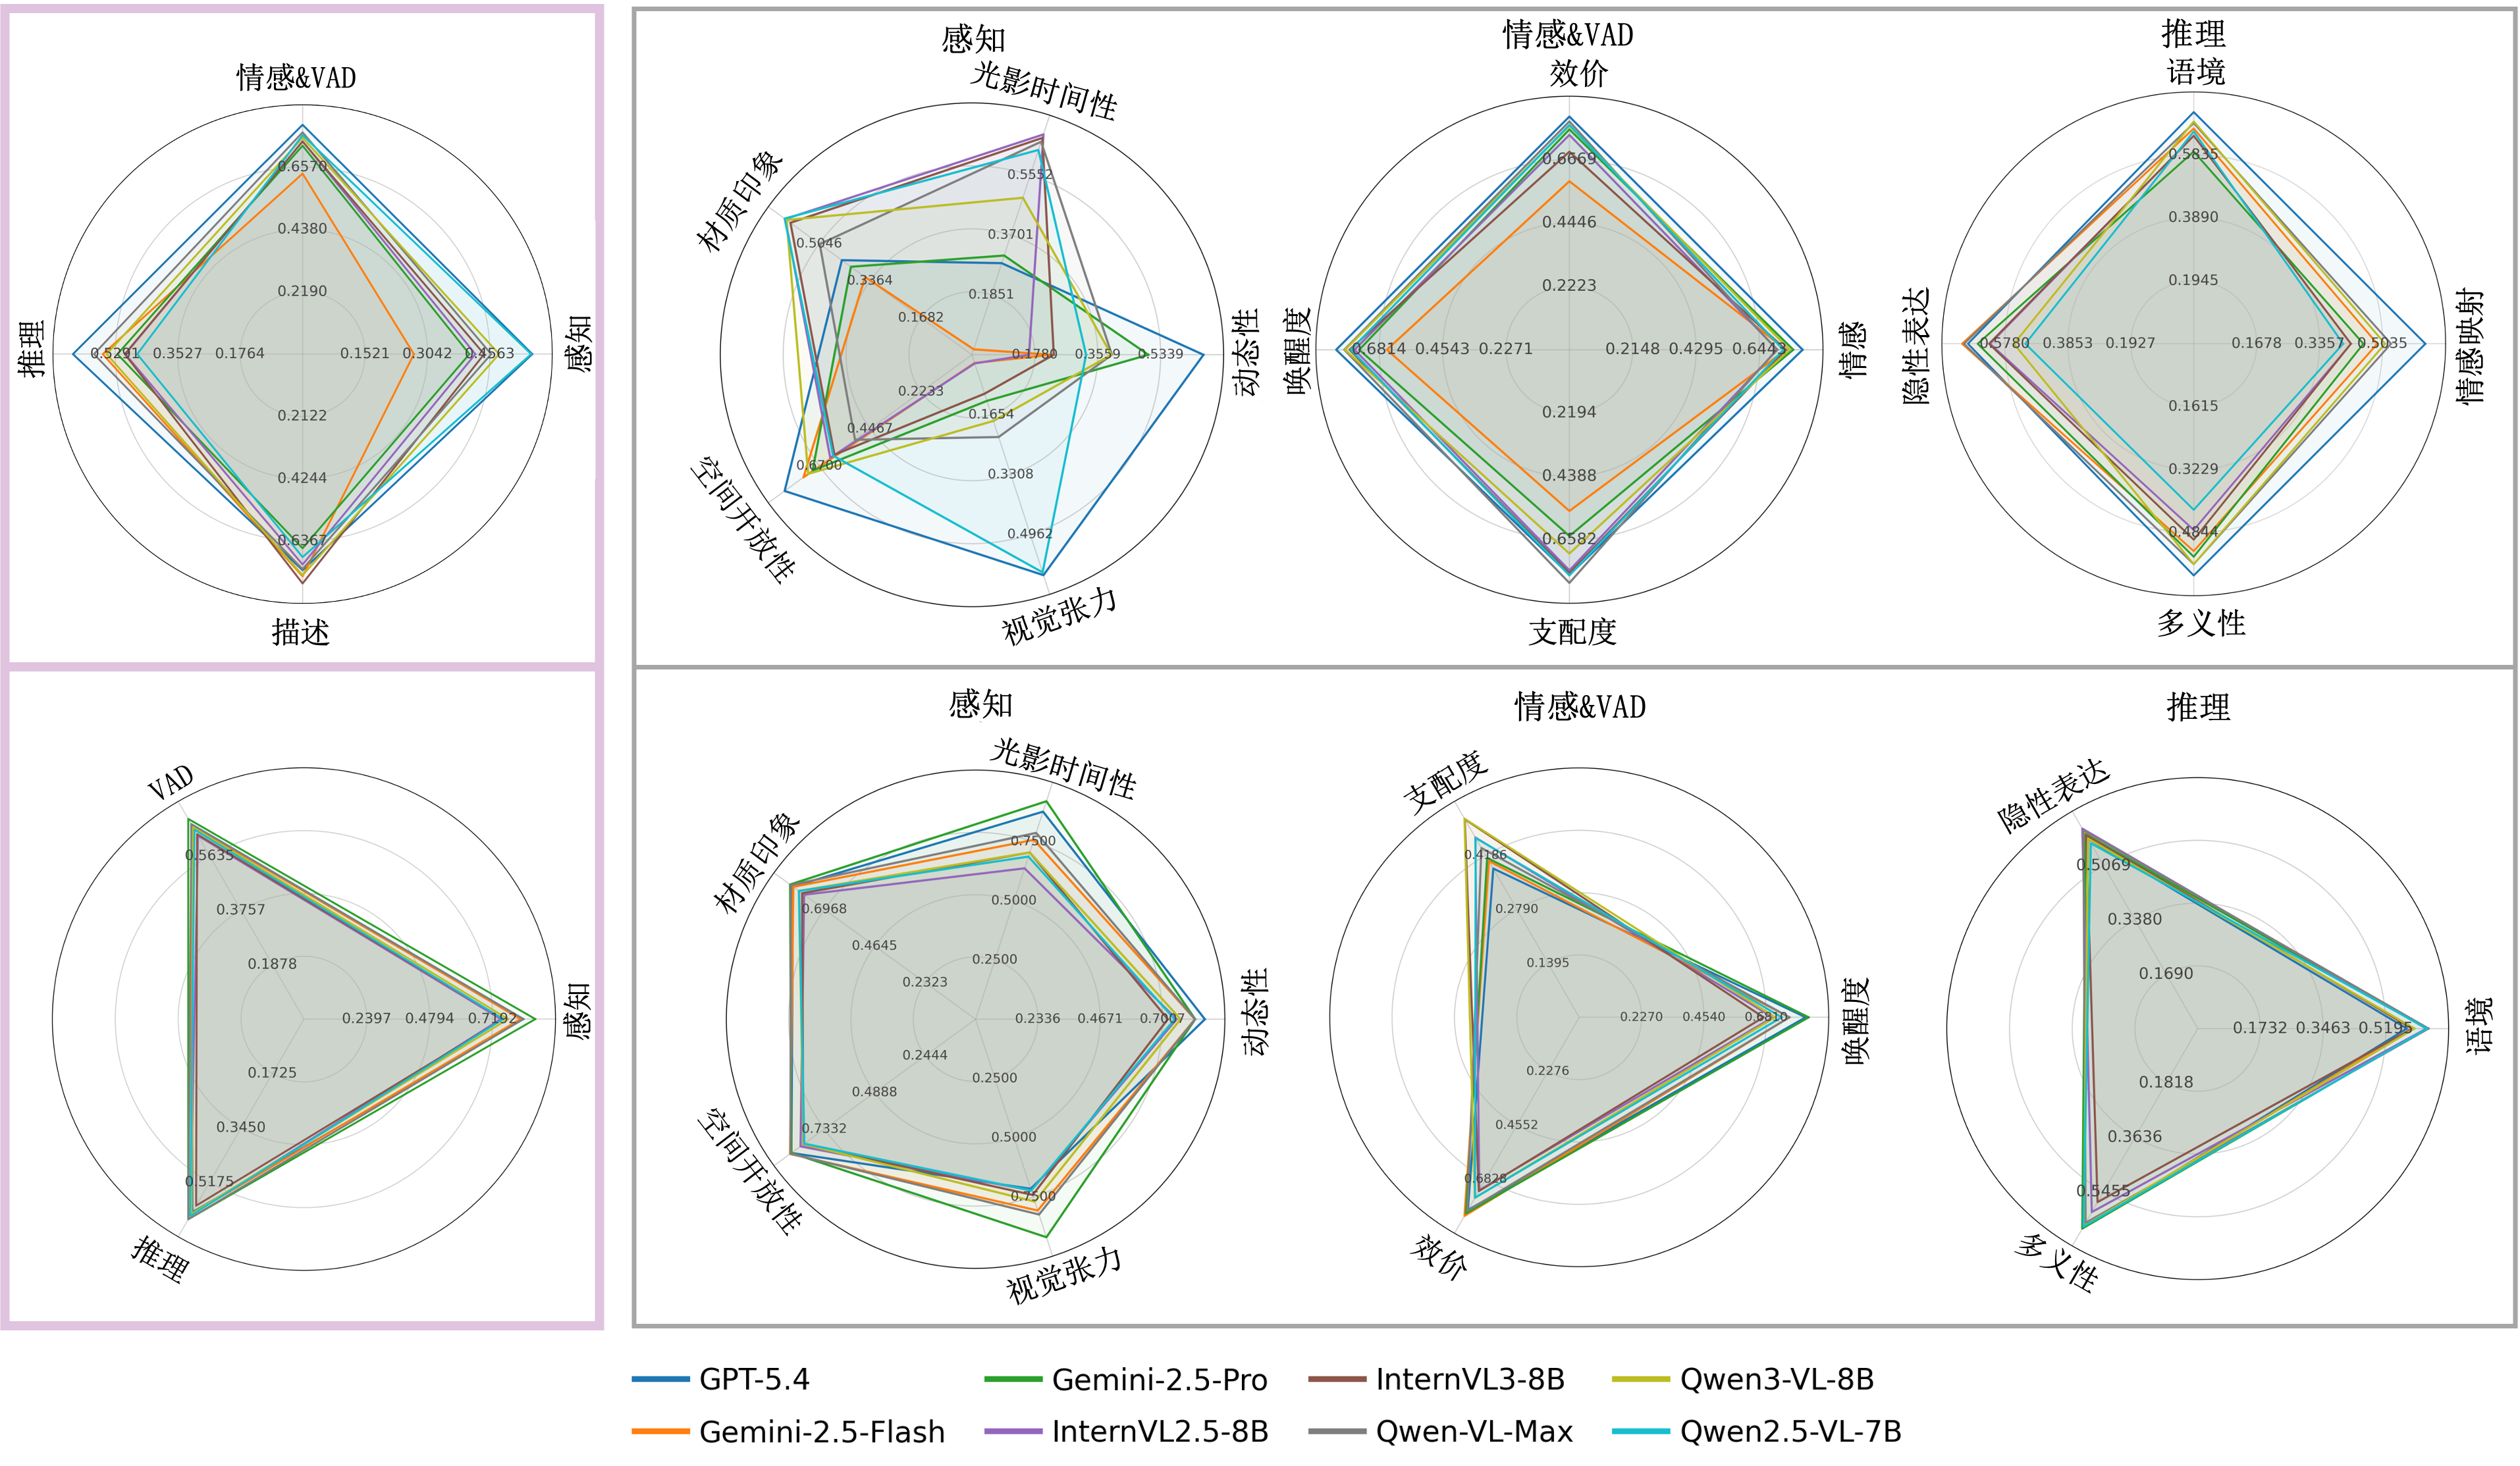
\includegraphics[width=0.95\textwidth]{figures/aerbench/radar_re.png}
    \bicaption[fig:chap5_radar]{}{代表性的8 个 MLLM 在单图与双图设置下的雷达图对比}{Fig.}{Radar plots for single-image (top row) and paired-image (bottom row) evaluations on eight representative models, including the top-4 closed-source and top-4 open-source MLLMs; the two plots on the left summarize core dimensions, while the six plots on the right show task-level performance per dimension}
\end{figure}



基于表~\ref{tab:chap5_main_results} 与图~\ref{fig:chap5_radar} 的系统评测结果，本节提炼出四项贯穿任务族与模型设置的核心发现，分别对应“感知—情感—推理”三级能力上的不同失效模式。

\begin{itemize}
\item 发现 1：情感标签比感知机制更容易。单图评测结果显示，情感与 VAD 预测在所有模型上都是表现最稳定的任务族：GPT-5.4 取得最高分 0.8760，Qwen-VL-Max 取得 0.8472，Qwen2.5-VL-7B 取得 0.8364，Qwen3-VL-8B 取得 0.8265。这说明 MLLM 已经能够相当可靠地识别作品的粗粒度情感倾向，并将作品映射到离散或连续的代表性情感表征。然而这一优势并未直接迁移到感知维度识别。即使是表现最佳的模型 GPT-5.4 与 Qwen2.5-VL-7B 在感知任务上也仅取得 0.6084 与 0.6054。图~\ref{fig:chap5_radar}（上行）进一步显示，模型在材质印象、空间开放性与光照时间性上的表现相对较好，而在动态性与视觉张力上的离散度显著更大。这一模式说明：静态或表层线索较易识别，而涉及“隐含运动、构图张力”等更专业的视觉属性则需要更专门的感知敏感度。因此，高情感/VAD 准确率不应被解读为完整的艺术理解：模型可能在不准确识别“支撑情感判断的感知机制”的情况下输出看似合理的情感状态。

\item 发现 2：流畅描述不保证基于证据的推理。 推理与描述任务揭示了模型能力上的互补短板。GPT-5.4 在单图推理上领先，Qwen-VL-Max 与 Gemini-2.5-Pro 紧随其后。情感/VAD 与推理之间的分数差表明：模型虽然常常能够给出看似合理的情感标签，但难以将这些标签构建为忠实于视觉证据、上下文线索与表达模式的解释。描述任务则呈现不同模式：Gemini-2.5-Flash 取得最高分 0.8226，Qwen3-VL-8B 也取得 0.8185，超过 GPT-5.4 的 0.8000。这说明流畅的情感化描述更多受益于通用生成能力与视觉摘要能力，而严格的推理要求更精确地将“声明”与“证据”对齐。推理雷达图（图~\ref{fig:chap5_radar} 上行右侧）进一步揭示了这一局限：上下文类推理相对较强，而感知—情感映射与歧义消解类推理仍显著薄弱。换言之，模型更擅长生成连贯的情感语言，而非解释“作品为何引发特定情感反应”。

\item 发现 3：对比有助于感知但无助于情感校准。双图评测为情感比较判断提供了独立测试。Gemini-2.5-Pro 在双图整体性能上取得最高分，其后依次为 Qwen-VL-Max、GPT-5.4、Gemini-2.5-Flash、Qwen3-VL-8B。相较于单图任务，头部模型在配对感知上的得分普遍提升——Gemini-2.5-Pro 达到 0.9589，GPT-5.4 达到 0.9100。这表明相对比较能够使显著的感知差异更易检出，尤其当两件作品在张力、空间开放性、运动或光照上形成直接对比时。但双图评测也暴露出情感校准上的持续困难：Gemini-2.5-Pro 取得最高 0.7514，开源模型中 Qwen3-VL-8B 取得 0.7200，但仍有多个模型得分低于 0.55。雷达图（图~\ref{fig:chap5_radar} 下行）也显示 Gemini-2.5-Flash 与 Gemini-2.5-Pro 在单图感知上偏弱，但在配对任务上表现强劲。这一对比表明 Gemini 系列更擅长识别“相对情感差异”，而在为单件作品赋予“绝对感知标签”时能力相对受限。因此，双图设置以测试关系型情感判断补充了单图评测，避免了模型仅依赖图像内在先验。

\begin{figure}[!htbp]
    \centering
    \subfigure[]{
        \includegraphics[width=0.95\textwidth]{papers/AER-Bench/figures/cases.pdf}
    }
    \hfill
    \subfigure[]{
        \includegraphics[width=0.95\textwidth]{papers/AER-Bench/figures/description_case.pdf}
        }
    \bicaption[fig:chap5_cases]{}{（a）推理与（b）描述任务的成功与失败定性案例}{Fig.}{Qualitative cases of success and failure patterns in affective reasoning and description. (a) reasoning cases; (b) description cases}
\end{figure}

\item 发现 4：主要瓶颈是基于证据的解释。 跨任务族来看，最强表现集中在情感/VAD 与配对感知上，而最大短板则出现在精细化感知与推理上。这一非对称性表明：当前 MLLM 更擅长给出“看似合理的情感标签或描述”，但在识别“支撑这些标签的中介感知机制”上仍存在系统性差距。上述结果支撑了 AER-Bench 的诊断动机：艺术情感理解不应仅以“模型是否预测出正确情感”作为评价基准，而应同时考察模型能否（1）识别相关的美学线索、（2）比较作品之间的情感差异、（3）将自身的解释组织为“基于证据的、有逻辑的陈述”。本基准因此揭示了当前 MLLM 的核心能力缺口：它们能够流畅地“谈论”情感，却仍难以将情感主张锚定到精确的视觉与上下文证据之上。
\end{itemize}

% \FloatBarrier

% \subsection{定性案例与经验启示}

% \label{sec:chap5_cases_insights}

图~\ref{fig:chap5_cases} 给出了 AER-Bench 推理与描述任务的代表性定性案例。推理案例覆盖了四类核心推理——上下文解释、情感歧义、表达模式、感知—情感映射——并不仅检验模型是否给出“看似合理的情感”，还检验其能否将视觉证据、上下文线索与情感概念整合为连贯的解释。描述案例进一步显示“流畅语言”不足以支撑可靠的情感理解：模型虽然生成了“冲突”“神秘”“荒凉”等看似贴切的情感短语，但遗漏或错位了若干关键视觉证据，包括锯齿状的线条、暗沉的色调、壕沟般的阻断、铁丝网般的形态、粗糙的肌理与压迫感的天空。与参考标注相比，模型输出抓住了“氛围片段”却未能将其组织为对 alarm、tension、frustration、entrapment、hostility、历史性创伤等情感的忠实证词支撑。

上述统计画像与多维发现共同指向三点核心启示。其一，从统计层面看，AER-Bench 在标签空间多样性、情感—VAD 内部一致性、感知—情感关联强度上同时具备可解释性，模型既不能仅依赖情感标签的先验偏置取得高分，也不能仅依赖通用视觉语义绕过艺术特有的中介线索。其二，从能力层面看，当前 MLLM 存在“情感识别强—感知机制弱”、“流畅描述强—证据推理弱”、“配对感知强—情感校准弱”三组非对称短板，其中“基于证据的解释”是最为普遍的能力瓶颈。其三，从诊断价值看，AER-Bench 通过将失败模式定位到上下文锚定、歧义消解、表达模式判断、感知—情感映射与描述综合等多个环节，能够为后续模型迭代提供独立的优化目标。

% \subsection{本节小结}

% 本节从“统计画像—系统评测—核心发现—定性案例”四个层次，给出了 AER-Bench 的完整分析结果。统计层面，基准在情感偏态分布、情感—VAD 内部一致性（$\epsilon^2 \geq 0.293$）与感知—情感共现结构（视觉张力 $V=0.5310$）上同时具备多样性、可解释性与诊断性；评测层面，14 个代表性 MLLM 在 AER-Bench 上的整体能力可被清晰刻画为“情感识别相对成熟、感知机制与证据推理显著薄弱”的能力非对称结构；发现层面，四项核心发现分别揭示了情感—感知的不对称、流畅—证据的不对称、相对—绝对判断的不对称以及“基于证据的解释”这一主要瓶颈；案例层面，定性证据进一步表明基准能够将“表层情感流畅”与“基于证据的解释”清晰区分，从而为后续艺术场景下的可解释视觉基础模型研究提供可扩展的诊断平台与改进方向。
\FloatBarrier

\section{本章小结}

本章围绕多模态大语言模型在艺术情感理解上的能力边界，构建了层级化任务体系与统一评测协议。在任务设计上，将艺术情感理解拆解为感知、情感、推理与描述四个互补层级，并将每一层级实例化为可重复生成的评测题目；在评测协议上，借助生成式模型辅助的结构化标注、相似度过滤与人工核验，并结合确定性度量和基于评分细则的语义评判，覆盖单图与配对两种设置。对 14 个代表性多模态大语言模型的系统评测表明，模型能够给出较可靠的情感判断或流畅描述，但基于视觉证据的解释仍是突出短板。与前文通过适应和先验融合提升跨域、跨类别迁移能力不同，本章不更新被评测模型，而是评估其面对更高层级语义任务时的能力适用范围，为后续模型迁移与优化明确可检验的目标。

% Local Variables:% Local Variables:
% TeX-master: "../thesis"
% TeX-engine: xetex
% End:


\backmatter
% !Mode:: "TeX:UTF-8"
\begin{conclusions}

视觉感知模型从训练条件走向目标场景时，既可能遭遇数据分布与类别词表的变化，也可能面对更高的任务语义要求。本文将模型在这些条件变化下仍需保持相应能力的情形统称为多泛化场景，沿域泛化、类泛化与语义理解泛化三个层面展开研究。研究对象由跨分布的样本表征、开放类别的概念识别，逐步拓展至高阶语义解释：前两个层面通过目标域适应与跨模型先验融合改善迁移表现，第三个层面则在不更新模型的条件下，以系统评测考察已有能力面对艺术情感推理任务时的适用范围。能力提升与能力评测由此构成本文两种不同而相互衔接的研究方式。

% 本文以视觉模型迁移为主线，沿域泛化、类泛化与语义理解泛化三个层面协同展开研究：域泛化层面贯穿第 2 章与第 3 章，分别沿卷积神经网络与状态空间模型两条骨干路径协同抑制数据域迁移不确定性，并进一步扩展至稀缺标注设定下的少监督迁移问题；类泛化层面对应第 4 章，面向开放词汇分割任务设计跨模型先验融合方法；语义理解泛化层面对应第 5 章，构建艺术情感推理的多层级评测协议以系统化诊断现有模型的语义理解能力。

（1）面向无监督跨域迁移，源模型依赖的域特异性线索可能使目标域表征与预测偏移；错误预测一旦被用作伪标签，又会在自训练中放大初始偏差。针对监督信号的可靠性，本文提出 UPA，利用特征空间的邻域一致性估计样本级伪标签可靠性，自适应筛选训练样本，并通过类别感知对比学习抑制噪声传播，无需引入额外的不确定性估计模型。针对骨干表征的稳定性，本文提出 SfMamba，以通道级视觉状态空间模块增强跨通道建模，并通过语义一致性打乱策略削弱背景空间共现带来的虚假相关性，在保持线性序列复杂度的同时建模长程依赖。两项工作分别从伪标签监督和特征表征环节减轻迁移误差的累积，在 Office、Office-Home、VisDA-C 与 DomainNet-126 等无源域适应基准上验证了有效性。

（2）面向少监督跨域迁移，有限标注能否有效覆盖目标域差异、并转化为目标模型的判别能力，是提高监督信息利用效率的关键。本文以固定监督预算下的目标域学习收益界定信息最大化目标，在无源主动域适应设定中提出 DAMF：通过双聚焦样本选择获取具有代表性和判别价值的目标样本，适配视觉—语言模型以提供互补语义监督，再通过交替蒸馏促进其与源模型之间的双向知识传递。协作风险上界从样本覆盖、模型风险与跨模型对齐等方面分析了方法的作用。在 Office-Home、VisDA-C 与 Office 的闭集和开集实验中，该方法相较所比较的基线取得了性能提升，表明有限标注与多模态先验的协同利用能够改善目标域适应。

（3）面向类泛化中的开放词汇分割任务，模型既要识别训练阶段未见的类别，也要准确确定其像素区域。现有方法往往难以兼顾视觉—语言模型的开放语义能力与分割基础模型的空间定位能力。本文提出 CMPF，在轻量解码器中通过查询注入和特征注入融合两类先验，并在推理阶段集成分割基础模型的零样本掩码预测，缓解类别判别与掩码质量之间的错配。该方法在全景、语义和实例分割等八个基准上验证了对未见类别的泛化能力。

（4）面向语义理解要求提升的艺术情感推理任务，已有研究分别提供了情感解释、视觉属性、刺激区域及多任务情感评测，但在同一评测体系中追踪视觉线索、情感判断与证据化解释之间的关系仍有不足。本文构建 AER-Bench，将艺术情感理解划分为感知维度、情感与效价—唤醒度—支配度、基于证据的推理和情感描述四个互补层级，结合单图与配对任务、确定性指标与开放式评分，对 14 个代表性多模态大语言模型进行系统评测。结果揭示模型的情感判断与证据化解释之间仍存在能力差距。本章通过评测刻画已有能力在高阶语义任务中的适用范围，并不将评测结果视作模型优化后的迁移增益。

综合上述工作，本文从跨分布条件下的可靠适应出发，进一步研究开放类别下的先验融合，并以高阶语义任务中的能力评测检验模型已有知识的适用范围。这一路径将稳定表征、未见类别识别与证据化语义解释置于同一目标条件变化的框架下，也明确区分了迁移方法带来的性能改进与评测所揭示的能力边界。

本文的实验主要在预设的目标域、类别集合与评测任务上展开，尚未覆盖目标条件持续变化的长期部署过程。后续研究可进一步考察分布漂移与新类别出现时的持续适应，兼顾新知识获取和已有能力保持；在标注稀缺、语义判断存在主观差异的任务中，建立能够区分模型失误、标注分歧与评测偏差的评价机制；并探索隐私与合规约束下的分布式知识迁移，使模型能够在数据无法集中汇集时仍获得可靠的适应能力。

\end{conclusions}


\bibliographystyle{hithesis}
\bibliography{reference}

% -*-coding: utf-8 -*-
%%%%%%%%%%%%%%%%%%%%%%%%%%%%%%%%%%%%%%%%%%%%%%%%%%%%%%%%%
\appendix
\chapter{协同SFADA风险上界证明}[协同SFADA风险上界证明]%
本附录给出第 3 章定理 3.4的完整证明。引理 3.1 与引理 3.2 给出的 UDA 与 SFDA 风险上界作为前置结论，其证明可见标准域适应理论文献~\cite{mathelin2022discrepancy}。
%%%%%%%%%%%%%%%%%%%%%%%%%%%%%%%%%%%%%%%%%%%%%%%%%%%%%%%%%
% \section{定理 3.4 的证明}[Proof of Theorem 3.4]
\label{app:theorem_3_4_proof}

\begin{proof}
由 $L$ 关于各变量的 $\mu$-Lipschitz 连续性与三角不等式，对所有 $x'\in \mathcal T$，$x\in \mathcal T_q$，目标模型风险可分解为
\begin{align}
\mathcal L_P(h,f_P) \ &\le\ \underbrace{\mathbb E_{x\sim P}L\big(f_P(x),f'_P(x)\big)}_{(A)}  + \underbrace{\mathbb E_{x\sim P}\!\big[L(f'_P(x),g(x))+L(g(x),h(x))\big]}_{(B)}.
\end{align}

\paragraph{控制项 (B)}
令 $g^\star\in\arg\min_g\max_{x\in\mathcal T}\big[L(f'_P(x),g(x))+L(g(x),h(x))\big]$，并记 $F_g(x):=L(f'_P(x),g(x))+L(g(x),h(x))$，则对任意 $x\in \mathcal T$ 有
\begin{equation}
F_g(x)\le \max_{u\in\mathcal T} F_g(u).
\end{equation}
按 $\eta_{\mathcal G}$ 的定义：
\begin{equation*}
\max_{u\in\mathcal T}F_{g^\star}(u)=\eta_{\mathcal G}.
\end{equation*}
对 $x\sim P$ 取期望并应用 Hoeffding / McDiarmid 不等式与对 $h$、$g$ 的联合 Rademacher 复杂度一致界，以至少 $1-\delta/3$ 的概率：
\begin{align}
(B)(g)=\mathbb E_{x\sim P}F_g(x) &\le \frac{1}{n_t}\sum_{x'\in \mathcal T}F_g(x') + 2\mu \big(\mathfrak R_{n_t}(\mathcal H)+ \mathfrak R_{n_t}(\mathcal G \circ\phi)\big)+\sqrt{\tfrac{M^2\log(3/\delta)}{2n_t}}.
\end{align}
将 $g^\star$ 代入，并利用 $\frac{1}{n}\sum_{x'\in \mathcal T}F_g(x')\le \max_{u\in\mathcal T}F_{g^\star}(u)=\eta_{\mathcal G}$，得
\begin{align}
(B) \ &\le\ \eta_{\mathcal G} \ +\ 2\mu\big(\mathfrak R_{n_t}(\mathcal H)+\mathfrak R_{n_t}(\mathcal G\circ\phi)\big) +\sqrt{\tfrac{M^2\log(3/\delta)}{2n_t}}.
\end{align}

\paragraph{控制项 (A)}
由经验均值的集中不等式，以至少 $1-\delta/3$ 的概率：
\begin{align}
(A) \ &\le\ \frac{1}{n_t}\sum_{x'\in\mathcal T}L\big(f_P(x'),f'_P(x')\big) \ +\ \sqrt{\tfrac{M^2\log(3/\delta)}{2n_t}}.
\end{align}
对 $x\in \mathcal T_q$，由引理3.3 并对 $x'$ 取平均：
\begin{align}
   \frac{1}{n_t}\sum_{x'\in\mathcal T} L\big(f_P(x'),f'_P(x')\big) &\le \frac{1}{|\mathcal T_q|}\sum_{x\in\mathcal T_q} L\big(f_P(x),f'_P(x)\big)\notag \\
   &\quad+\frac{\mu}{n_t}\sum_{x'\in\mathcal T}\Big(k d_X(x',x)+ k_V d_Z\big(\phi(x'),\phi(x)\big)\Big).
\end{align}
由于上式对任意 $x\in\mathcal T_q$ 成立，特别地可取 $x\in\mathcal T_q$ 使 $x$ 尽量接近 $x'$，从而
\begin{align}
   \frac{1}{n_t}\sum_{x'\in\mathcal T} L\big(f_P(x'),f'_P(x')\big) &\le \frac{1}{|\mathcal T_q|}\sum_{x\in\mathcal T_q} L\big(f_P(x),f'_P(x)\big)\notag \\
   &\quad+\frac{\mu}{n_t}\sum_{x'\in\mathcal T}\Big(k d_X(x',\mathcal T_q)+ k_V d_Z\big(\phi(x'),\mathcal T_q\big)\Big).
\end{align}

合并 (A) 与 (B) 的上界，并对三个 $\delta/3$ 事件取并集，以至少 $1-\delta$ 的概率：
\begin{align}
    \mathcal L_{P}(h,f) &\le\mathcal L_{\hat Q}(f_P,f'_P)+\frac{\mu}{n_t}\sum_{x'\in\mathcal T}\!\Big(k d_X(x',\mathcal T_q)+k_V d_Z(\phi(x'),\mathcal T_q)\Big) \notag\\
    &\quad+\eta_{\mathcal G}+2\mu\big(\mathfrak R_{n_t}(\mathcal H)+\mathfrak R_{n_t}(\mathcal G\!\circ\!\phi)\big) +2\sqrt{\tfrac{M^2\log(3/\delta)}{2n_t}}.
\end{align}
即式~\eqref{eq:collab_bound}，定理3.4 证毕。
\end{proof}


% -*-coding: utf-8 -*-*
%%%%%%%%%%%%%%%%%%%%%%%%%%%%%%%%%%%%%%%%%%%%%%%%%%%%%%%%%
% 附录 B：章节计数器承接附录 A，不重复 \appendix（否则计数器被重置回 0）
\chapter{AER-Bench 标注协议}[Details of annotation and reliability for AER-Bench]
\label{app:aerbench_supplement}
本附录给出第 5 章 AER-Bench 的GPT-4o标注对象划分、字段级模式与取值约束的完整定义，以及标注的人工核验细节。
%%%%%%%%%%%%%%%%%%%%%%%%%%%%%%%%%%%%%%%%%%%%%%%%%%%%%%%%%

% \section{LLM 评判的可靠性核验}
% \label{app:llm_judge_validation}

% 本节验证大语言模型评判能否作为专家评分细则评判的可扩展代理。评测过程中抽取 360 条模型响应，单图推理、配图推理与情感描述三类任务各 120 条。三位具有视觉艺术、艺术史与多模态评测背景的专家，使用与模型评判完全相同的 0--2 评分细则对每条响应打分。为保证同一基准下的可比性，专家与模型评判仅接收同一份纯文本评测包，即任务提示、候选响应与参考答案，且对来源模型与评判分数保持盲态。

% 核验结果给出在正文表~\ref{tab:chap5_llm_judge}中，本节说明其读法。模型评判与专家中位分数之间的二次加权 Cohen's $\kappa_w$ 达到 0.60；在同一批响应上重复评判五次，得到整体自我一致性 $\alpha=0.86$。单图推理、配图推理与情感描述三类任务上的模型--人类 $\kappa_w$ 序列依次为 0.69、0.58、0.53，与标注平均得分序列 0.89、0.77、0.72 单调平行，说明评判在任务之间的方差差异反映的是各任务固有的判别难度，而非评判者的偶发偏好。据此可以认为模型评判在语义正确性、相关性、推理质量与关键证据覆盖四个维度上足以替代人工专家承担开放式题的常规评判。

% \section{标注细节}
\label{app:annotation_protocol}

% \subsection{标注协议与结构化输出模式}

\paragraph{标注规则}
AER-Bench 的全部标注对象遵循以下规则。
\begin{itemize}
    \item 针对给定的 \texttt{image\_id} 返回且仅返回一个符合模式的对象，其中须包含五个感知字段（$\mathcal{O}_{\text{per}}$）、情感归因（$\mathcal{O}_{\text{emo}}$）、推理字段（$\mathcal{O}_{\text{rea}}$）与描述字段（$\mathcal{O}_{\text{des}}$），不允许出现额外字段；
    \item $\mathcal{O}_{\text{des}}$ 与 $\mathcal{O}_{\text{rea}}$ 中的每一项关键论断都必须落到具体视觉证据上，证据可以是物体、姿态或手势、光线方向、色彩对比、笔触或肌理以及空间层次，不允许出现缺乏图像锚点的抽象论断；
    \item 标注不得虚构作品的元信息。
\end{itemize}

% \paragraph{输出对象与允许取值}
输出模式与 AER-Bench 的四级基准层级一一对应。表~\ref{tab:app_annotation_objects} 先给出每个顶层标注对象在基准层级中的语义角色，表~\ref{tab:app_annotation_schema} 随后给出完整的字段级模式，涵盖允许取值与生成约束。

\begin{table}[!htbp]
    \centering
    \bicaption[tab:app_annotation_objects]{}{顶层标注对象及其在基准层级中的角色}{Table}{Top-level annotation objects and their roles in the benchmark taxonomy}
    \vspace{0.4em}\wuhao
    \setlength{\tabcolsep}{5pt}
    \renewcommand{\arraystretch}{1.15}
    \begin{tabularx}{\textwidth}{@{}p{0.08\textwidth}p{0.24\textwidth}X@{}}
    \toprule
    对象 & 基准角色 & 必需内容 \\
    \midrule
    $\mathcal{O}_{\text{per}}$ & 情感线索感知 & 五个视觉--情感维度，即视觉张力、动态性、空间开放性、材质印象与光照时间性 \\
    $\mathcal{O}_{\text{emo}}$ & 情感归因 & 排序后的 Top-3 情感预测，以及效价--唤醒度--支配度（VAD）评分 \\
    $\mathcal{O}_{\text{rea}}$ & 解释性推理 & 由感知线索到情感的映射、语境解释、情感歧义分析与表达模式分析 \\
    $\mathcal{O}_{\text{des}}$ & 情感描述 & 对作品整体情感氛围的、忠实且有证据支撑的自然语言综合 \\
    \bottomrule
    \end{tabularx}
\end{table}

\begin{table}[!htbp]
    \centering
    \bicaption[tab:app_annotation_schema]{}{完整的字段级标注模式与生成约束}{Table}{Complete field-level annotation schema and generation constraints}
    \vspace{0.4em}\zihao{-5}
    \setlength{\tabcolsep}{5pt}
    \renewcommand{\arraystretch}{1.15}
    \begin{tabularx}{\textwidth}{@{}p{0.16\textwidth}p{0.34\textwidth}X@{}}
    \toprule
    基准组成 & 允许取值或长度约束 & 标注规则 \\
    \midrule
    \multicolumn{3}{@{}l}{\itshape \textbf{情感线索感知（$\mathcal{O}_{\text{per}}$）}} \\
    视觉张力 & \{低, 中, 高\} & 构图张力、对比、拥挤或视觉应力的程度 \\
    动态性 & \{静止, 中等, 动态\} & 隐含的或被描绘的运动程度 \\
    空间开放性 & \{封闭, 均衡, 开放\} & 构图在观感上封闭、均衡或向外延展的程度 \\
    材质印象 & \{冷调技术, 中性, 温暖自然\} & 材质与类温度的主导印象 \\
    光照时间性 & \{静态, 轻微变化, 强周期\} & 光照在感知上的时间变化或周期性 \\
    \midrule
    \multicolumn{3}{@{}l}{\itshape \textbf{情感归因（$\mathcal{O}_{\text{emo}}$）}} \\
    情感排序 & \{兴奋, 激动, 快乐, 悲伤, 无聊, 疲惫, 惊恐, 恼怒, 沮丧, 高兴, 满足, 平静\} & 从共享的 12 词情感词表中选取恰好三个并排序 \\
    VAD & 效价、唤醒度、支配度 $\in\{1,2,3,4,5\}$ & 三个维度得分须与感知标注及情感标注保持一致 \\
    \midrule
    \multicolumn{3}{@{}l}{\itshape \textbf{解释性推理（$\mathcal{O}_{\text{rea}}$）}} \\
    情感映射 & 1--3 条陈述，每条不少于 140 个字符 & 说明一到两个感知维度如何支撑情感归因，须给出具体视觉证据 \\
    语境解释 & \{历史, 文化, 宗教, 政治, 象征, 无\}；适用时说明不少于 120 个字符 & 说明所选语境如何改变对作品情感的解释 \\
    情感歧义 & \{多实体, 主体--背景, 形式--内容, 模糊, 无\}；适用时说明不少于 120 个字符 & 说明相互竞争的情感线索，并为双方的判断各给出视觉证据 \\
    表达模式 & \{直接, 间接, 混合, 无\}；适用时说明不少于 120 个字符 & 说明情感是通过直接、间接还是混合策略传达的 \\
    \midrule
    \multicolumn{3}{@{}l}{\itshape \textbf{情感描述（$\mathcal{O}_{\text{des}}$）}} \\
    情感描述与综合 & 一段不少于 480 个字符的描述 & 通过具体形式、物体、手势、光线、色彩、构图或肌理综合作品的情感氛围，不允许出现无证据支撑的纯情绪化表述 \\
    \bottomrule
    \end{tabularx}
\end{table}

作为补充，$\mathcal{O}_{\text{emo}}$ 对象中的三个情感标签按最显著到第三显著排序。VAD 的锚点固定如下：效价从强负向（1）到强正向（5），3 表示中性或混合情感；唤醒度从非常平静或低激活（1）到高度激活或强烈（5），3 表示中等激活；支配度从非常无力或被支配（1）到强烈掌控（5），3 表示控制程度处于平衡水平。

$\mathcal{O}_{\text{rea}}$ 对象实例化的是正文定义的四种推理类型，不引入额外的推理类别。特别地，对情感映射而言，每一条都包含一段自然语言陈述与一份 $\mathcal{O}_{\text{per}}$ 引用列表，后者指向一到两个感知字段；该陈述不少于 140 个字符，且必须引用具体视觉证据。对三种可选推理类型，取值为无表示该类型不适用于该作品。

\paragraph{人工核验}
\label{app:human_verification}

三位专家标注员对分层随机抽取的 360 个实例独立审计，三类任务各 120 个实例。该审计是随机样本上的只读质量审计，而非第二轮标注。对每个实例，标注员沿一致性维度给出 0--2 的序数评分，其中 0 表示存在明显问题，1 表示存在轻微问题，2 表示可接受。一致性指已发布的推理、描述与标注是否在可见作品上彼此吻合，并锚定于上游的感知维度与情感及 VAD 维度。
% 审计结果给出在正文表~\ref{tab:chap5_llm_judge}的标注核验部分。
% % !Mode:: "TeX:UTF-8"

\begin{publication}
\noindent\textbf{（一）发表的相关论文}

\begin{publist}
\item 一作. AER-Bench: A Benchmark for Emotion Perception and Reasoning in Fine Art[J]. IEEE Transactions on Affective Computing (\textbf{TAC}), 2026, pp.1-13. （EI, SCI, DOI: 10.1109/TAFFC.2026.3730731, IF: 11.3, 中科院1区TOP, JCR1区, CCF-B类期刊, 第5章）
\item Sicheng Zhao, \textbf{Xi Chen(共一)}, Hongxun Yao, Haosen Yang, Yanhao Zhang, Sheng Jin, Xiatian Zhu, Haonan Lu, Kui Jiang, Guiguang Ding. CMPF: Harmonizing Cross-Model Prior Fusion for Open-Vocabulary Segmentation[J]. International Journal of Computer Vision (\textbf{IJCV}), 2026, 134. （EI, SCI: 001779020700002, DOI: 10.1007/s11263-026-02886-0, IF: 10.3, 中科院2区，JCR1区, CCF-A类期刊, 第4章）
\item \textbf{Xi Chen}, Hongxun Yao, Sicheng Zhao, Jiankun Zhu, Jing Jiang, Kui Jiang. SfMamba: Efficient Source-Free Domain Adaptation via Selective Scan Modeling[J]. Expert Systems with Applications (\textbf{ESWA}), 2026, 324, pp.132421. （EI, SCI: 001759382000001, DOI: 10.1016/j.eswa.2026.132421, IF: 9.4, 中科院1区TOP, JCR1区, CCF-B类期刊，第2章）
\item \textbf{Xi Chen}, Haosen Yang, Huicong Zhang, Hongxun Yao and Xiatian Zhu. Uncertainty-aware Pseudo-label Filtering for Source-Free Unsupervised Domain Adaptation[J]. Neurocomputing, 2024, 575, pp.127190.（EI, SCI: 001172429800001, DOI: 10.1016/j.neucom.2023.127190, IF: 6.7, 中科院2区, JCR1区, CCF-C类期刊, 第2章）
\item \textbf{Xi Chen}, Hongxun Yao, Zhaopan Xu, Kui Jiang. DAM: Dual Active Learning with Multimodal Foundation Model for Source-Free Domain Adaptation[C]. IEEE International Conference on Acoustics, Speech and Signal Processing (\textbf{ICASSP}), 2026, pp. 5841-5845. （EI, DOI: 10.1109/ICASSP55912.2026.11463823, CCF-B类会议，第3章）
\end{publist}


\noindent\textbf{（二）在投的相关论文}

Xi Chen, Hongxun Yao, Zhaopan Xu, Sheng Jin, Sicheng Zhao, Kui Jiang. Data-Active Multimodal Fusion for Source-Free Domain Adaptation[J]. Information Fusion, 2026. (EI, SCI, IF: 17.4, 中科院1区TOP, JCR1区). （第3章）

\noindent\textbf{（三）已获得的专利}

% ===== 以下为非盲审原始内容，保留备用 =====
 姚鸿勋，陈希，张慧琮. 一种基于多基础大模型的开放词表分割方法. 发明专利, 2025.

\noindent\textbf{（四）参与的科研项目及获奖情况}

姚鸿勋等。农场环境自适应感知与认知技术研究，科技创新2030“新一代人工智能”重大项目。课题编号：2021ZD0110901。

% ===== 以下为非盲审原始内容，保留备用 =====
% \item 姚鸿勋等。农场环境自适应感知与认知技术研究，科技创新2030“新一代人工智能”重大项目。课题编号：2021ZD0110901。
%\vfill
%\hangafter=1\hangindent=2em\noindent
%\setlength{\parindent}{2em}
\end{publication}

% !Mode:: "TeX:UTF-8"

\begin{publication}
\noindent\textbf{（一）发表的相关论文}

\begin{publist}
\item 一作. IEEE Transactions on Affective Computing (\textbf{TAC}), 2026. （EI, SCI, IF: 11.3, 中科院1区TOP, JCR1区, CCF-B类期刊, 第5章）
\item 学生一作. International Journal of Computer Vision (\textbf{IJCV}), 2026, 134. （EI, SCI, IF: 10.3, 中科院2区，JCR1区, CCF-A类期刊, 第4章）
\item 一作. Expert Systems with Applications (\textbf{ESWA}), 2026, 324. （EI, SCI, IF: 9.4, 中科院1区TOP, JCR1区, CCF-B类期刊，第2章）
\item 一作. Neurocomputing, 2024, 575.（EI, SCI, IF: 6.7, 中科院2区, JCR1区, CCF-C类期刊, 第2章）
\item 一作. IEEE International Conference on Acoustics, Speech and Signal Processing (\textbf{ICASSP}), 2026. （EI, CCF-B类会议，第3章）
\end{publist}


\noindent\textbf{（二）在投的相关论文}

一作. Information Fusion, 2026. (EI, SCI, IF: 17.4, 中科院1区TOP, JCR1区). （第3章）

\noindent\textbf{（三）已获得的专利}

% ===== 以下为非盲审原始内容，保留备用 =====
学生一作, 发明专利, 2025.

\noindent\textbf{（四）参与的科研项目及获奖情况}

姚鸿勋等。农场环境自适应感知与认知技术研究，科技创新2030“新一代人工智能”重大项目。课题编号：2021ZD0110901。

% ===== 以下为非盲审原始内容，保留备用 =====
% \item 姚鸿勋等。农场环境自适应感知与认知技术研究，科技创新2030“新一代人工智能”重大项目。课题编号：2021ZD0110901。
%\vfill
%\hangafter=1\hangindent=2em\noindent
%\setlength{\parindent}{2em}
\end{publication}


% 博士答辩决议表（以下三种用法择一）：
\resolution               % 电子版
%\resolution[scan.pdf]    % 使用扫描件，不添加页码（扫描件中已有页码时使用）
%\resolution*[scan.pdf]   % 使用扫描件，自动添加页码（扫描件中无页码时使用）

% \begin{ceindex}
  %如果想要手动加索引，注释掉以下这一样，用wordlist环境
\printsubindex*
\end{ceindex}


% 授权（以下三种用法择一）：
\authorization             % 电子版
%\authorization[scan.pdf]  % 使用扫描件，不添加页码（扫描件中已有页码时使用）
%\authorization*[scan.pdf] % 使用扫描件，自动添加页码（扫描件中无页码时使用）

% !Mode:: "TeX:UTF-8"
\begin{acknowledgements}
值此论文完成之际，回顾从本科入学到今日博士论文定稿的这段求学时光，心中满是感激。

衷心感谢我的导师姚鸿勋教授。从研究方向的选定、方法的推敲到论文的逐字修改，姚老师始终给予我耐心而具体的指导。他对研究问题的敏锐判断、对技术细节的严谨要求、以及在论文写作与投稿过程中给予的悉心指点，让我受益良多。姚老师严谨求实的治学态度与宽厚待人的处世方式，是我一生学习的榜样。

感谢哈尔滨工业大学计算机科学与技术专业的各位任课教师，是他们为我的专业基础提供了支撑。感谢计算学部提供的良好学习环境、丰富的学术资源与自由的探索氛围，使我得以安心读书、潜心科研。

感谢实验室的同门师兄师姐与师弟师妹们。感谢师兄们在模型训练、实验调试与论文修改各环节提供的无私帮助，感谢同窗们在日常讨论与并肩奋斗中给予的鼓励与陪伴。感谢华为技术有限公司诺亚实验室的实习经历，使我得以接触工业界对视觉技术落地的真实需求，并由此更加深刻地理解本文工作的实际意义。

感谢我的家人。父母始终是我坚实的后盾，他们的理解、宽容与无条件支持，是我能够心无旁骛完成学业的根本保障。感谢亲友在漫长求学过程中的鼓励与陪伴。


谨以此文献向所有关心和帮助过我的师长、同学、朋友和家人表示最诚挚的谢意！
\end{acknowledgements}

% !Mode:: "TeX:UTF-8"

\begin{resume}
    陈希，女，1998年10月14日出生，山东省菏泽市人，中共党员。主要研究领域为人工智能、计算机视觉和多模态理解。攻读博士学位期间，围绕模型迁移泛化、多模态微调与多模态大模型评测等方向开展研究。以第一作者身份发表5篇SCI/CCF学术论文。

\noindent\textbf{教育经历}

    2021年9月------至今 \qquad      哈尔滨工业大学，计算机科学与技术专业，博士研究生

    2020年9月------2021年6月     \qquad  哈尔滨工业大学，计算机科学与技术专业，硕士研究生

    2016年9月------2020年6月   \qquad   哈尔滨工程大学，计算机科学与技术专业，本科

\noindent\textbf{工作经历}：

2022 年11月------2023 年4 月 \qquad 华为技术有限公司，诺亚实验室，算法实习生
    
\end{resume}

\end{document}
